\documentclass[11pt,oneside]{book}
\usepackage{fontspec}
\setmainfont{Noto Serif}
\setsansfont{Noto Sans}
\setmonofont{Noto Sans Mono}
\newfontfamily\proseunicodefont{DejaVu Serif}
\usepackage[margin=1in]{geometry}
\usepackage{microtype}
\usepackage{amsmath,amssymb,amsthm,mathtools,bm}
\usepackage{graphicx}
\usepackage{adjustbox}
\usepackage{xcolor}
\usepackage{booktabs}
\usepackage{array}
\usepackage{longtable}
\usepackage{enumitem}
\usepackage{float}
\usepackage{caption}
\usepackage{hyperref}
\usepackage{fancyhdr}
\usepackage{tikz}
\usetikzlibrary{arrows.meta,positioning,calc,decorations.pathmorphing}

\hypersetup{
  colorlinks=true,
  linkcolor=blue!50!black,
  urlcolor=blue!50!black,
  citecolor=blue!50!black
}

\setlength{\parskip}{0.5em}
\setlength{\parindent}{0pt}
\setlist[itemize]{topsep=0.25em,itemsep=0.2em}
\setlist[enumerate]{topsep=0.25em,itemsep=0.2em}
\setlength{\headheight}{40pt}
\numberwithin{equation}{chapter}

\newtheorem{theorem}{Теорема}[chapter]
\newtheorem{proposition}[theorem]{Утверждение}
\newtheorem{lemma}[theorem]{Лемма}
\newtheorem{corollary}[theorem]{Следствие}
\theoremstyle{definition}
\newtheorem{definition}[theorem]{Определение}
\newtheorem{example}[theorem]{Пример}
\theoremstyle{remark}
\newtheorem{remark}[theorem]{Замечание}

\providecommand{\ket}[1]{\left\lvert#1\right\rangle}
\providecommand{\bra}[1]{\left\langle#1\right\rvert}
\providecommand{\braket}[2]{\left\langle#1\,\middle|\,#2\right\rangle}
\providecommand{\expect}[1]{\left\langle#1\right\rangle}
\newcommand{\lectureoverview}[1]{\paragraph{Обзор.} #1}

\makeatletter
\newcommand{\course@headerfont}{\normalfont\small\itshape}
\newcommand{\course@pagefont}{\normalfont\small}
\newcommand{\course@headerraise}{14pt}
\newlength{\course@headerboxheight}
\setlength{\course@headerboxheight}{\dimexpr\headheight-\course@headerraise-9pt\relax}
\newcommand{\course@leftheadbox}[1]{%
  \raisebox{\course@headerraise}{%
    \parbox[t][\course@headerboxheight][t]{0.82\textwidth}{%
      \raggedright\course@headerfont\strut\MakeUppercase{#1}\strut%
    }%
  }%
}
\newcommand{\course@rightheadbox}[1]{%
  \raisebox{\course@headerraise}{%
    \parbox[t][\course@headerboxheight][t]{0.82\textwidth}{%
      \raggedleft\course@headerfont\strut\MakeUppercase{#1}\strut%
    }%
  }%
}
\renewcommand{\chaptermark}[1]{\markboth{\MakeUppercase{\chaptername\ \thechapter.\ #1}}{}}
\renewcommand{\sectionmark}[1]{\markright{\MakeUppercase{\thesection\hspace{0.4em}#1}}}
\fancyhf{}
\fancyhead[L]{\course@leftheadbox{\leftmark}}
\fancyhead[R]{\course@pagefont\thepage}
\renewcommand{\headrulewidth}{0.5pt}
\pagestyle{fancy}
\fancypagestyle{plain}{%
  \fancyhf{}
  \fancyhead[L]{\course@leftheadbox{\leftmark}}
  \fancyhead[R]{\course@pagefont\thepage}
  \renewcommand{\headrulewidth}{0.5pt}
}
\makeatother

% Video2Book editorial provenance macros
\newenvironment{classroomqa}{%
  \par\medskip\noindent\begin{minipage}{\linewidth}\small\hrule\medskip
}{%
  \medskip\hrule\end{minipage}\par\medskip
}
\newcommand{\audiencequestion}[1]{\noindent\textbf{Вопрос из аудитории.} #1\par\smallskip}
\newcommand{\lecturerresponse}[1]{\noindent\textbf{Ответ.} #1\par}
\newcommand{\lecturetimestamp}[1]{\footnote{Время в лекции: #1.}}
\newcommand{\lectureframe}[1]{\par\smallskip{\centering\footnotesize\itshape Кадр лекции: #1.\par}}
\newcommand{\editorialnote}[1]{\footnote{Редакторское пояснение: #1}}

\usepackage{polyglossia}
\setdefaultlanguage{russian}
\usepackage{sectsty}
\renewcommand{\contentsname}{Содержание}
\renewcommand{\chaptername}{Глава}
\renewcommand{\figurename}{Рисунок}
\renewcommand{\tablename}{Таблица}
\renewcommand{\proofname}{Доказательство}
\renewcommand{\bibname}{Литература}
\sectionfont{\raggedright}
\subsectionfont{\raggedright}
\makeatletter
\renewcommand{\@pnumwidth}{2.2em}
\renewcommand{\@tocrmarg}{3.2em}
\makeatother
\usepackage{tocloft}
\renewcommand{\cftchapfont}{\small\bfseries}
\renewcommand{\cftchappagefont}{\small\bfseries}
\renewcommand{\cftsecfont}{\small}
\renewcommand{\cftsecpagefont}{\small}
\setlength{\cftsecnumwidth}{3em}
\renewcommand{\cftsubsecfont}{\small}
\renewcommand{\cftsubsecpagefont}{\small}
\setlength{\cftsubsecindent}{4.5em}
\setlength{\cftsubsecnumwidth}{4em}
\emergencystretch=6em
\pdfstringdefDisableCommands{\def\proseunicodefont{}}

\geometry{paperwidth=177.6mm,paperheight=252mm,left=16mm,right=16mm,
 top=18mm,bottom=18mm,includeheadfoot,headheight=28pt,headsep=7mm,footskip=9mm}
\usepackage{scrextend}
\changefontsizes[17pt]{12pt}
\raggedbottom
\renewenvironment{classroomqa}{\par\medskip\begingroup}{\par\endgroup\medskip}
\fancyhf{}
\setlength{\headwidth}{\textwidth}
\fancyhead[L]{\parbox{\textwidth}{\raggedright\fontsize{9}{11}\selectfont\nouppercase{\leftmark}}}
\fancyfoot[C]{\small\thepage}
\renewcommand{\headrulewidth}{0.3pt}
\fancypagestyle{plain}{\fancyhf{}\fancyfoot[C]{\small\thepage}\renewcommand{\headrulewidth}{0pt}}

\graphicspath{{../../../generated_course_notes/supplementary/particle_physics_2_standard_model/2010_winter/figures/}{../../../generated_course_notes/supplementary/particle_physics_2_standard_model/2010_winter/assets/}}
\begin{document}
\frontmatter
\hypersetup{pageanchor=false}
\begin{titlepage}
\hyphenpenalty=10000\exhyphenpenalty=10000
\thispagestyle{empty}
\begin{tikzpicture}[remember picture,overlay]
  \node[anchor=center,inner sep=0] at (current page.center) {%
    \includegraphics[height=\paperheight,keepaspectratio]{../../../generated_course_notes/supplementary/particle_physics_2_standard_model/2010_winter/assets/cover-art.png}%
  };
  \node[
    anchor=north west,
    align=left,
    text width=0.78\paperwidth,
    fill=white,
    fill opacity=0.9,
    rounded corners=8pt,
    inner xsep=10pt,
    inner ysep=8pt
  ] at ([xshift=0.08\paperwidth,yshift=-0.06\paperheight]current page.north west) {%
    {\fontsize{30}{33}\selectfont\bfseries\color{black!88} Физика элементарных частиц 2: стандартная модель\\[0.85em]}
    {\large\color{black!72} Русское издание / зима 2010}
  };
  \node[
    anchor=south west,
    align=left,
    text width=0.68\paperwidth,
    fill=white,
    fill opacity=0.82,
    text opacity=1,
    rounded corners=6pt,
    inner sep=12pt
  ] at ([xshift=0.08\paperwidth,yshift=0.08\paperheight]current page.south west) {%
    {\normalsize\color{black!78} Оригинальные лекции: Leonard Susskind\\[0.35em]}
    {\small\color{black!72} Сопроводительное издание: \href{https://lazying.art}{LazyingArt LLC} / \href{https://github.com/lachlanchen/Video2Book}{Video2Book}}
  };
\end{tikzpicture}
\mbox{}
\end{titlepage}
\hypersetup{pageanchor=true}

\clearpage
\chapter*{Об этих заметках}
Эти независимо отредактированные сопроводительные конспекты составлены по лекциям Леонарда Сасскинда. Они были восстановлены по машинным расшифровкам, субтитрам и выбранным кадрам с доски, а затем сверены с доступными исходными материалами. Это не оригинальная рукопись профессора Сасскинда, и она не была им ни рассмотрена, ни одобрена.

Издание было подготовлено \href{https://lazying.art}{LazyingArt LLC} с использованием рабочего процесса с открытым исходным кодом \href{https://github.com/lachlanchen/Video2Book}{Video2Book}. Машинные расшифровки по-прежнему доступны отдельно и могут содержать ошибки распознавания. Редакторские уточнения и нетривиальные реконструкции отмечены в сносках.
\clearpage
\tableofcontents
\mainmatter
\chapter{Силы, кварки и первые адронные мультиплеты}

\section{Частицы, поля и недостающая третья сторона}

Волны представляют собой конфигурации полей, так что в нашем обсуждении эти два описания тесно связаны. Квантовая механика утверждает, что энергия в такой волне приходит дискретными, неделимыми порциями. Эти порции — её кванты, а кванты поля — это то, что мы называем его частицами. Имея в виду эту связь, мы уже обсудили волновые уравнения, принципы действия и общие свойства, переносимые частицами: энергию, импульс, спин и бозон--фермионное различие. Фермионы противятся занятию одного и того же состояния; бозоны могут собираться и конденсироваться в одном состоянии.

Квантовый лагранжиан также фиксирует взаимодействия. Произведения полей соответствуют вершинам, в которых частицы входят и выходят. Член, содержащий, например, четвёртую степень поля, представляет четырёхлучевую вершину взаимодействия. Так принцип действия превращается в компактный перечень возможных процессов с частицами.

Следующая задача — назвать частицы---не совсем по одной, а по семействам---и придать им некоторую индивидуальность: их свойства, их взаимодействия и их место в обычной физике. Однако прежде чем составить этот список, в одном концептуальном треугольнике всё ещё недостаёт одной стороны:
\begin{itemize}
\item частицы,
\item поля, квантами которых являются эти частицы,
\item силы, связанные с процессами обмена с участием тех же самых квантов.
\end{itemize}

Слово \emph{элементарный} пока должно оставаться предварительным. Любое правдоподобное определение элементарной, а не составной частицы в конце концов наталкивается на неоднозначный случай, и к этой проблеме мы ещё вернёмся. Пока же предположим, что фундаментальные поля существуют, и будем называть их кванты элементарными частицами. Если электрическое поле порождает электрические силы, а гравитационное поле — гравитационные силы, то и поле электрона тоже должно участвовать в силовых взаимодействиях. Треугольник может замкнуться, только если у силы есть описание не только в терминах поля, но и в терминах частиц.

Поэтому мы дважды выведем логику силы. Сначала воспользуемся классической энергией поля; затем спросим, как то же самое взаимодействие выглядит, когда поле разлагается на кванты. Лишь после того, как этот мост будет надёжно установлен, начнётся каталог частиц.

\section{Сила из энергии поля в классической электродинамике}

Поместим в пространстве два заряда. Один способ найти действующую между ними силу — сослаться на закон обратных квадратов. Более содержательный способ — спросить, что заряды делают с пространством: они создают электрические поля, а эти поля запасают энергию.

Полезно отделить каждый заряд от пространственной формы его поля,
\begin{equation}
\mathbf E_i=q_i\widehat{\mathbf E}_i,
\end{equation}
хотя от сохранения обозначения со шляпкой ничего не зависит. При наличии обоих зарядов линейность даёт
\begin{equation}
\mathbf{E}=\mathbf{E}_1+\mathbf{E}_2.
\end{equation}
С точностью до выбора единиц энергия электростатического поля имеет вид
\begin{equation}
U_{\text{field}}\propto\int d^3x\,\mathbf{E}^2.
\end{equation}
Подставляя сумму двух полей, получаем
\begin{align}
U_{\text{field}}
&\propto\int d^3x\,(\mathbf{E}_1+\mathbf{E}_2)^2 \\
&\propto\int d^3x\,\bigl(\mathbf{E}_1^2+\mathbf{E}_2^2
  +2\mathbf{E}_1\!\cdot\!\mathbf{E}_2\bigr).
\end{align}

Первые два члена — это собственные энергии. Перенос любого из зарядов переносит вместе с ним и его поле и не изменяет соответствующий интеграл. Эта энергия через \(E=mc^2\) вносит вклад в измеряемую массу изолированной заряженной частицы. То, как эта собственная энергия включается в измеряемую массу, относится к более поздней теме перенормировки. Никакая часть этой не зависящей от положения энергии не вносит вклада в силу между двумя частицами.

Перекрёстный член устроен иначе. Он не принадлежит отдельно ни одной из частиц и существует только тогда, когда присутствуют оба поля. Если разнести заряды очень далеко, области, где их поля заметны, почти не перекрываются. Когда заряды сближаются, перекрытие меняется. Поэтому энергия взаимодействия, зависящая от конфигурации, пропорциональна
\begin{equation}
U_{\text{int}}(r)\propto q_1q_2\int d^3x\,
\widehat{\mathbf E}_1\!\cdot\!\widehat{\mathbf E}_2.
\end{equation}
Для двух точечных зарядов, разделённых расстоянием \(r\), вычисление интеграла даёт привычную зависимость
\begin{equation}
U_{\text{int}}(r)\propto\frac{q_1q_2}{r}.
\end{equation}
Радиальная сила равна её отрицательному градиенту,
\begin{equation}
\mathbf F_{12}=-\boldsymbol\nabla_{\mathbf r}U_{\text{int}},
\qquad
|\mathbf F_{12}|\propto\frac{|q_1q_2|}{r^2}.
\end{equation}
\editorialnote{Устный аргумент отождествляет перекрёстный член с кулоновской силой, подчиняющейся закону обратных квадратов, не задерживаясь на потенциале. Стандартное промежуточное выражение \(U_{\mathrm{int}}\propto1/r\) здесь выписано явно, так что его градиент даёт указанную силу \(1/r^2\).}

Закон силы стал производной той части энергии поля, которая зависит от относительного положения. Когда два объекта далеко друг от друга, они фактически независимы. Если сблизить их, поле между ними перестраивается; возникающее изменение энергии и есть взаимодействие.

Но если поле можно разложить на кванты, на этом история не заканчивается. У той же самой силы должно быть и описание на языке частиц.

\section{Молекулярный обмен: два протона и один электрон}

Прежде чем вернуться к электродинамике, рассмотрим систему, в которой обмен легче себе представить: два протона и один электрон. Обмен — лишь один из нескольких источников молекулярных сил, но этот пример делает наглядной связь между обменом, энергией и силой. Он не предлагается как замена квантовой электродинамике.

Если присутствует один протон, а другой находится бесконечно далеко, электрон может занимать водородоподобное основное состояние с центром на первом протоне. Его волновая функция локализована вблизи этого силового центра.

\begin{figure}[h]
\centering
\includegraphics[width=0.72\textwidth]{lecture_01_figure_02.png}

\medskip

\begin{tikzpicture}[scale=0.95]
\draw (-0.2,0) -- (6.4,0);
\fill (1.3,0) circle (2pt);
\draw[smooth] plot coordinates {(0.1,0.15) (0.8,1.15) (1.5,1.75) (2.2,1.1) (3.0,0.35) (3.8,0.12)};
\node at (1.3,-0.35) {$p$};
\node at (2.7,1.55) {$\psi_1(x)$};
\end{tikzpicture}
\caption{Волновая функция водородоподобного основного состояния, локализованная около одного протона.}
\lectureframe{00:14:32}
\end{figure}
\editorialnote{Метка \(\psi_1(x)\) на перерисованном рисунке обозначает локализованный профиль, описанный в 00:14:30--00:14:32; она не скопирована с разборчивой подписи на доске.}

Теперь поместим второй протон на большое, но конечное расстояние. По симметрии существует второе локализованное состояние с той же одноцентровой энергией, на этот раз с центром на правом протоне.

\begin{figure}[h]
\centering
\includegraphics[width=0.78\textwidth]{lecture_01_figure_03.png}

\medskip

\begin{tikzpicture}[scale=0.92]
\draw (-0.2,0) -- (9.0,0);
\fill (1.4,0) circle (2pt);
\fill (7.4,0) circle (2pt);
\draw[smooth] plot coordinates {(0.2,0.2) (0.9,1.05) (1.6,1.55) (2.4,1.0) (3.3,0.35) (4.2,0.12)};
\draw[smooth] plot coordinates {(4.8,0.12) (5.7,0.35) (6.6,1.0) (7.3,1.55) (8.1,1.05) (8.8,0.2)};
\node at (1.4,-0.35) {$p$};
\node at (7.4,-0.35) {$p$};
\node at (2.6,1.45) {$\psi_1(x)$};
\node at (6.2,1.45) {$\psi_2(x)$};
\end{tikzpicture}
\caption{Два локализованных профиля, из которых составляется равновесная суперпозиция после того, как туннелирование становится возможным.}
\lectureframe{00:17:54}
\end{figure}
\editorialnote{Метки \(\psi_1(x)\) и \(\psi_2(x)\) обозначают два профиля, обсуждаемые в 00:17:41--00:17:56; эти символы представляют собой схематические метки, добавленные для наглядности.}

При бесконечном расстоянии между ними два состояния вырождены: локализация электрона слева или справа требует одной и той же энергии. При конечном расстоянии становится возможным новый процесс. Электрон может туннелировать через классически запрещённую область от одного центра к другому. Попытка проследить траекторию через барьер возмутила бы состояние; ``перескок'' — это описание квантовой эволюции, а не фильм классической траектории.

В равновесии вероятность обнаружить электрон вблизи любого из протонов одинакова. Поэтому нормировка даёт множитель \(1/\sqrt2\), и более низкое по энергии равновесное состояние приблизительно равно
\begin{equation}
\psi_+(x)\approx \frac{\psi_1(x)+\psi_2(x)}{\sqrt2}.
\end{equation}

Знак приближения здесь существен. Истинная двухцентровая волновая функция не является в точности суммой двух невозмущённых водородоподобных орбиталей; в области перекрытия она подстраивается. Для нас здесь важно, что симметричное равновесное состояние лежит ниже изолированной одноцентровой энергии. На языке гамильтониана левая и правая конфигурации связаны недиагональным матричным элементом. Если позволить электрону занимать их когерентную суперпозицию, энергия понижается.

\section{От понижения энергии к эффективной силе}

При большом расстоянии между протонами индуцированный электроном вклад \(E_e(r)\) стремится к своему значению для разделённых атомов. При меньшем расстоянии туннелирование и суперпозиция понижают его. Полный потенциал системы двух протонов--одного электрона должен также содержать прямое отталкивание протонов,
\begin{equation}
V_{\mathrm{tot}}(r)=V_{pp}(r)+E_e(r).
\end{equation}

Это вновь связывает молекулярный пример с рассуждением об энергии поля. Эскизы волновой функции и качественная кривая для \(E_e(r)\) — это два взгляда на один и тот же расчёт; равновесие определяется суммой \(V_{\mathrm{tot}}(r)\).

\begin{figure}[h]
\centering
\includegraphics[width=0.78\textwidth]{lecture_01_figure_04.png}

\medskip

\begin{tikzpicture}[scale=0.9]
\draw (-0.2,3.0) -- (9.0,3.0);
\fill (1.3,3.0) circle (2pt);
\fill (7.3,3.0) circle (2pt);
\draw[smooth] plot coordinates {(0.1,3.15) (0.9,4.0) (1.7,4.45) (2.6,3.9) (3.7,3.25) (4.6,3.08)};
\draw[smooth] plot coordinates {(4.8,3.08) (5.9,3.25) (7.0,3.9) (7.8,4.45) (8.6,4.0) (9.0,3.15)};
\node at (1.3,2.65) {$p$};
\node at (7.3,2.65) {$p$};

\draw[->] (0.2,0.1) -- (0.2,2.0);
\draw[->] (0.2,0.1) -- (8.8,0.1);
\draw[dashed] (0.5,1.48) -- (8.5,1.48);
\draw[smooth] plot coordinates {(0.5,0.38) (1.6,0.56) (2.8,0.82) (4.1,1.08) (5.5,1.27) (6.9,1.39) (8.4,1.44)};
\node at (5.8,1.02) {$E_e(r)$};
\node at (8.8,-0.18) {$r$};
\end{tikzpicture}
\caption{Перекрытие волновых функций вверху и индуцированная электроном энергия внизу. При увеличении \(r\) она поднимается к асимптоте разнесённых атомов; полный потенциал протонов должен также включать их кулоновское отталкивание.}
\lectureframe{00:20:28}
\end{figure}
\editorialnote{Метки \(E_e(r)\) и \(r\) обозначают энергетическую кривую и расстояние, обсуждаемые в 00:19:12--00:20:38; сохранившийся кадр доски не позволяет разобрать эти подписи осей.}

Две соответствующие силы следуют из градиентов энергии,
\begin{equation}
F_{e}(r)=-\frac{dE_e}{dr},
\qquad
F_{\mathrm{tot}}(r)=-\frac{dV_{\mathrm{tot}}}{dr}.
\end{equation}
Тем самым система подталкивается к меньшей полной энергии. Там, где \(E_e(r)\) уменьшается при сближении протонов, обмен даёт притягивающий вклад; существует ли связанное расстояние, зависит от его конкуренции с \(V_{pp}(r)\). Это элементарный механизм, лежащий в основе ковалентной связи: электрон оказывается общим, потому что обобществлённое состояние энергетически выгодно.

В классическом расчёте перекрытие электрических полей изменяет энергию. Здесь два силовых центра допускают более низкое квантовое состояние. Оба механизма порождают силу, потому что равновесная энергия зависит от конфигурации.

Язык обмена можно подытожить схемой мировых линий. Ее нельзя понимать как наблюдаемую траекторию; она представляет амплитуды того, что электрон связан либо с одним, либо с другим протоном.

\begin{figure}[h]
\centering
\begin{tikzpicture}[scale=1.0]
\draw (0,0) -- (0,4.4);
\draw (4.8,0) -- (4.8,4.4);
\draw (0,0.9) .. controls (1.6,1.7) and (3.2,1.7) .. (4.8,2.5);
\draw (4.8,2.9) .. controls (3.2,2.1) and (1.6,2.1) .. (0,3.9);
\node at (0,-0.35) {$p$};
\node at (4.8,-0.35) {$p$};
\node at (2.35,1.55) {$e^-$};
\node at (2.35,2.55) {$e^-$};
\end{tikzpicture}
\caption{Обмен электроном между двумя мировыми линиями протонов, понимаемый как схема квантовых амплитуд, а не как наблюдаемая траектория.}
\end{figure}

\begin{classroomqa}
\audiencequestion{Можно ли понимать это притяжение просто как экранирование электроном протонного заряда или уменьшение его величины?\lecturetimestamp{00:23:26}}
\lecturerresponse{Нет. Уменьшение заряда — неправильная картина для этого эффекта. Существенный факт состоит в том, что сложение двух локализованных волновых функций дает состояние с немного меньшей энергией, чем каждое из локализованных состояний по отдельности.}
\end{classroomqa}

\begin{classroomqa}
\audiencequestion{Это ли имел в виду Фейнман, говоря, что ``свет любит свет''?\lecturetimestamp{00:23:51}}
\lecturerresponse{Нет. Эта фраза, скорее всего, относится к бозе-статистике: фотоны предпочитают общие состояния, тогда как электроны подчиняются запрету. Молекулярный эффект здесь — это туннелирование между двумя центрами.}
\end{classroomqa}

Два протона по-прежнему электростатически отталкиваются. Обмен имеет меньший радиус действия, чем кулоновское взаимодействие, поэтому нужно рассматривать полный потенциал, а не каждый из вкладов по отдельности. Тем не менее при подходящих расстояниях молекулярный ион \(\mathrm H_2^+\) связан; в нейтральной двухэлектронной системе дальнодействующее зарядовое отталкивание отсутствует, и ковалентное связывание там еще более привычно.

\begin{classroomqa}
\audiencequestion{Главный ли эффект помещения электрона между протонами состоит в уменьшении их электростатического отталкивания?\lecturetimestamp{00:24:33}}
\lecturerresponse{Это немного уменьшает отталкивание, но не в этом состоит главный эффект. Обмен электроном — сила с меньшим радиусом действия, чем кулоновское отталкивание. Он наиболее заметен в нейтральной двухэлектронной системе, где дальнодействующая электростатическая сила между атомами отсутствует, но туннелирование все еще порождает притяжение.}
\end{classroomqa}

\begin{classroomqa}
\audiencequestion{Действительно ли положительно заряженный молекулярный ион \(\mathrm H_2^+\), имеющий только один электрон, связан?\lecturetimestamp{00:26:06}}
\lecturerresponse{Да. При достаточно малом расстоянии обменное притяжение достаточно сильно, чтобы преодолеть кулоновское протон--протонное отталкивание.}
\end{classroomqa}

\begin{classroomqa}
\audiencequestion{Создает ли двухцентровая конфигурация третью силу?\lecturetimestamp{00:26:24}}
\lecturerresponse{Нет, никакая новая фундаментальная сила не вводится. Уравнение Schr\"odinger в суммарном потенциале двух протонов имеет равновесную энергию, отличную от энергии в одноцентровой задаче; производная этой измененной энергии и есть эффективная сила.}
\end{classroomqa}

\begin{classroomqa}
\audiencequestion{Является ли понижение энергии примером квантовой запутанности?\lecturetimestamp{00:27:06}}
\lecturerresponse{Не в обычном двухчастичном смысле: нужен только один электрон. Существенной математической особенностью здесь является внедиагональный матричный элемент гамильтониана, связывающий левое и правое состояния.}
\end{classroomqa}

\begin{classroomqa}
\audiencequestion{Что происходит с обменом при высокой температуре?\lecturetimestamp{00:27:37}}
\lecturerresponse{При экстремально высокой температуре электрон ионизуется и совсем забывает о молекуле. При меньшей энергии возбуждения он может занять более протяженную орбиталь, изменяя перекрывание и, следовательно, силу. Это зависящая от состояния поправка, а не новый общий механизм.}
\end{classroomqa}

\section{Обмен фотонами и первые записи таблицы}

Можно ли описать кулоновскую силу на том же языке обмена? Заряженная частица взаимодействует с электромагнитным полем, кванты которого — фотоны. Классически мы находим электрическое поле вокруг заряда. В квантовой теории поля мы разлагаем это взаимодействие на испускание и поглощение фотонов.

Физическая заряженная частица — это не просто голый заряд. Ее состояние представляет собой квантовую суперпозицию, содержащую компоненту голого электрона, электрона с одним фотоном, электрона с двумя фотонами и так далее. В намеренно схематической записи,
\begin{equation}
\begin{aligned}
\ket{e_{\mathrm{phys}}}
={}&a_0\ket e
+a_1\ket{e+\text{one photon}}
\\
&+a_2\ket{e+\text{two photons}}+\cdots .
\end{aligned}
\end{equation}
Эта запись отражает только иерархию компонент с разным числом фотонов; она не задает импульсов фотонов и не претендует на полное построение взаимодействующего заряженного состояния.
Окружающие фотоны испускаются и вновь поглощаются, а не уходят как свободное излучение. Их эффекты можно измерить, хотя детектируют их не так, как свободно распространяющиеся фотоны. Если поместить рядом второй заряд, фотон, испущенный одним зарядом, может быть поглощен другим. Тогда энергия этих двух одетых состояний перестает быть равной простой сумме двух изолированных энергий.

Аудиторная аналогия — это два жонглера, каждый со своим набором мячей. Когда они далеко друг от друга, каждый жонглирует независимо. Стоит подвести их достаточно близко, и один может поймать мяч, брошенный другим. На языке диаграмм Фейнмана этот общий объект — обмениваемый фотон. Аналогия не изображает микроскопическую траекторию, но передает, почему близость делает возможным новый процесс.

Теперь у нас есть два описания, выходящие за рамки простого заучивания закона Кулона. Классическая теория поля складывает поля и возводит результат в квадрат. Квантовая теория поля суммирует амплитуды, в которых обмениваются кванты. В этом смысле частицы, поля и силы образуют взаимно-однозначное соответствие. Электроны опосредуют молекулярный обмен, фотоны — электромагнитный обмен, и любая частица, которой можно обмениваться, может в подходящей ситуации вносить вклад в силу. Поэтому привычное утверждение, что в природе есть 4 фундаментальных взаимодействия, является классификацией на более широком уровне; в рамках языка обмена каждый вид частиц, которым может идти обмен, может порождать собственный вклад в эффективную силу.

Наконец пришло время назвать частицы, перечислить их свойства и сказать, в каких процессах они могут участвовать. Если выписать всю стандартную модель сразу, получится лишь длинная проверка памяти, поэтому мы разобьем частицы на небольшие группы, члены которых просто связаны друг с другом, и разберем, что может делать каждая группа.

Полный каталог громоздок, потому что мы не понимаем, почему существуют именно эти частицы, тогда как другие мыслимые частицы не существуют. Математическая согласованность задает некоторые связи: если существует несколько членов некоторой схемы, для ее завершения может потребоваться еще один. Эти связи уменьшают число независимых фактов, но лишь в умеренной степени. Многие типы частиц и многие параметры остаются необъясненными. Понимание этой незавершенной структуры необходимо, чтобы понять, что пытаются обнаружить последующие эксперименты.

\begin{figure}[h]
\centering
\includegraphics[width=0.7\textwidth]{lecture_01_figure_05.png}
\caption{Первая запись в таблице частиц обозначает фотон символом \(\gamma\), а его поле — векторным потенциалом \(A\).}
\lectureframe{00:39:11}
\end{figure}

Первое соответствие поле--квант имеет вид
\begin{equation}
\gamma \leftrightarrow A.
\end{equation}
Здесь \(A\) — электромагнитный векторный потенциал. Фотон — бозон со спином 1, нулевым электрическим зарядом, нулевым барионным числом и нулевой массой покоя. Электронное поле принято обозначать \(\psi_e\); его компоненты рождения и уничтожения действуют на состояния электрона и позитрона.

В нашей таблице указаны название, символ частицы, поле, тип — бозон или фермион, электрический заряд \(Q\), барионное число \(B\) и масса:

\begin{table}[h]
\centering
\resizebox{\linewidth}{!}{%
\begin{tabular}{lllllll}
Название & Символ & Поле & Тип & \(Q\) & \(B\) & Масса \\
Фотон & \(\gamma\) & \(A\) & бозон & \(0\) & \(0\) & \(0\) \\
Электрон & \(e^-\) & \(\psi_e\) & фермион & \(-1\) & \(0\) & \(0.51\,\mathrm{MeV}\) \\
Позитрон & \(e^+\) & \(\psi_e\) & фермион & \(+1\) & \(0\) & \(0.51\,\mathrm{MeV}\)
\end{tabular}
}%
\caption{Записи для фотона и электрона--позитрона, которыми начинается каталог частиц.}
\end{table}

Электрон и позитрон связаны взаимно: каждый является античастицей другого. Называть отрицательно заряженное состояние ``частицей'' — условность. Электрический заряд измеряют в единицах модуля заряда электрона, поэтому
\begin{equation}
Q(e^-)=-1,\qquad Q(e^+)=+1.
\end{equation}
Массу измеряют в единицах энергии, используя \(E=mc^2\). Один электрон-вольт — это энергия, приобретаемая зарядом \(e\) при прохождении разности потенциалов в один вольт,
\begin{equation}
1\,\mathrm{eV}=e\,(1\,\mathrm V).
\end{equation}
Эта единица естественно возникает в атомной физике: в качестве грубой атомной шкалы ионизация водорода требует примерно \(13.5\,\mathrm{eV}\). Для масс частиц нужны миллионы или миллиарды электрон-вольт. Масса электрона равна
\begin{equation}
m_e c^2 \approx 0.511\,\mathrm{MeV}.
\end{equation}

\begin{classroomqa}
\audiencequestion{Должна ли масса электрона быть в точности равна половине МэВ?\lecturetimestamp{00:44:02}}
\lecturerresponse{Нет. Удобное округленное значение \(0.51\,\mathrm{MeV}\) не фиксируется никаким принципом как точная половина; это измеряемый параметр.}
\end{classroomqa}

В элементарном процессе КЭД одна линия заряженного фермиона входит, одна выходит, и к ним присоединена одна фотонная линия. Перестановка или кроссинг внешних линий позволяет той же вершине описывать испускание фотона, его поглощение или процесс с позитроном. В используемой здесь нековариантной схематической записи взаимодействие содержит
\begin{equation}
\mathcal{L}_{\mathrm{int}}\sim e\,\psi_e^\dagger \psi_e A.
\end{equation}
Разложение полей по операторам рождения и уничтожения даёт члены, которые уничтожают входящий электрон, создают выходящий электрон и создают или уничтожают фотон. Константа связи \(e\) даёт в вершине один множитель. Поэтому при испускании фотона, когда электрон рассеивается или ускоряется,
\begin{equation}
\mathcal{A}_{\mathrm{vertex}}\propto e,
\qquad
P_{\mathrm{emission}}\propto e^2.
\end{equation}
Один из практических случаев, где важна эта вероятность испускания фотона, — когда электрон попадает в мишень в рентгеновской трубке. Повторные сочетания той же вершины порождают процессы квантовой электродинамики, включая сдвиг энергии, интерпретируемый как сила между зарядами.

Поэтому такая схематическая вершина полезна.

\begin{figure}[h]
\centering
\begin{tikzpicture}[scale=1.0]
\fill (0,0) circle (1.5pt);
\draw (-1.6,-1.2) -- (0,0) -- (1.6,-1.2);
\draw (0,0) -- (0,1.8);
\node at (-1.8,-1.4) {$e^-$};
\node at (1.8,-1.4) {$e^-$};
\node at (0.35,1.95) {$\gamma$};
\end{tikzpicture}
\caption{Топологическая схема элементарной вершины КЭД: одна линия заряженного фермиона входит, одна выходит, и присоединён один фотон. Прямая фотонная линия здесь служит лишь упрощённым условным изображением.}
\end{figure}

Обменный вклад в силу связывает две такие вершины:

\begin{figure}[h]
\centering
\begin{tikzpicture}[scale=1.0]
\draw (0,0) -- (0,4.0);
\draw (4.8,0) -- (4.8,4.0);
\draw (0,2.0) -- (4.8,2.0);
\node at (0,-0.35) {$e^-$};
\node at (4.8,-0.35) {$e^-$};
\node at (2.4,2.3) {$\gamma$};
\end{tikzpicture}
\caption{Топологическая схема обмена фотоном, дающая квантово-полевое описание кулоновского взаимодействия.}
\end{figure}

Теперь, когда треугольник частица--поле--сила замкнут, можно продолжить каталог.

\section{Кварки, барионное число и загадка семейств}

Если бы этот каталог составлялся около 1960 года, за электронами и фотонами, вероятно, шли бы протоны и нейтроны. В современной физике элементарных частиц сначала вводят кварки. В наивной картине составляющих протоны и нейтроны представляют собой сравнительно большие составные объекты, построенные из более мелких кварковых степеней свободы. Точный смысл слова \emph{составной} ещё предстоит выяснить, но язык составляющих уже чрезвычайно полезен.

Все кварки — фермионы. Они несут барионное число, величину, введённую в ядерной физике при подсчёте нуклонов. \emph{Нуклон} означает конкретно протон или нейтрон. \emph{Барион} — более широкий класс, включающий нуклоны и похожие тяжёлые частицы, которые встретятся далее. Протон и нейтрон имеют по одной единице,
\begin{equation}
B(p)=B(n)=1,
\qquad
B(\bar p)=B(\bar n)=-1.
\end{equation}
Для ядра этот счёт барионов в точности совпадает с массовым числом \(A=Z+N\), то есть с числом протонов плюс нейтронов. Численное значение атомной массы, измеренной в атомных единицах массы, лишь приблизительно равно \(A\). В бета-процессах протоны могут превращаться в нейтроны, а нейтроны — в протоны, но общее число нуклонов не меняется. Например,
\begin{equation}
n\longrightarrow p+e^-+\bar\nu_e
\end{equation}
изменяет числа протонов и нейтронов по отдельности, сохраняя их сумму.

\begin{classroomqa}
\audiencequestion{Противоречат ли изотопы сохранению суммы числа протонов и нейтронов?\lecturetimestamp{00:52:03}}
\lecturerresponse{В разных изотопах действительно содержится разное число нейтронов, и бета-распад может превращать нейтрон в протон и наоборот. В обычном ядерном процессе сохраняющейся величиной является полное барионное число, а не число частиц каждого из этих видов по отдельности.}
\end{classroomqa}

Нормировка условна. Мы могли бы приписать протону барионное число \(2\), \(7\) или \(\pi\), если бы каждая составная частица масштабировалась согласованно. После того как протону приписано \(B=1\) и он содержит 3 кварка, каждый кварк должен нести
\begin{equation}
B(q)=\frac13,
\qquad
B(\bar q)=-\frac13.
\end{equation}
Таким образом, дробное значение является историческим следствием того, что сначала нормировали составной нуклон.

\begin{classroomqa}
\audiencequestion{Сохраняется ли число кварков?\lecturetimestamp{00:54:23}}
\lecturerresponse{Пары кварк--антикварк могут рождаться и уничтожаться, так что само по себе это число не сохраняется. Величина, соответствующая барионному числу, — это число кварков минус число антикварков, делённое на 3. Эмпирически она сохраняется с чрезвычайно высокой точностью, хотя здесь не предполагается, что это абсолютный закон.}
\end{classroomqa}

Гипотетический распад с сохранением заряда, такой как
\begin{equation}
p\longrightarrow e^++\gamma
\end{equation}
переводил бы барионное число 1 в конечное состояние с нулевым барионным числом. Этот канал приведён лишь как иллюстративный пример учёта, а не как предлагаемая модель распада. Ни одного процесса с нарушением барионного числа не наблюдалось. Приведённая здесь грубая граница помещает время жизни протона как минимум в диапазон \(10^{33}\)--\(10^{34}\) лет. Никто не наблюдает один-единственный протон так долго; наблюдают огромное число протонов в течение приемлемого времени, компенсируя длительность жизни размером выборки. Тем не менее распад протона широко ожидался, и ничто в обсуждаемой здесь математике не давало абсолютного запрета. Поэтому вопрос о том, сохраняется ли барионное число в точности, оставался открытым экспериментальным вопросом: нарушений не наблюдали, ограничения были жёсткими, но возможность не отвергалась.

\begin{classroomqa}
\audiencequestion{Нарушает ли аннигиляция протон--антипротон барионное число?\lecturetimestamp{00:56:17}}
\lecturerresponse{Нет. Начальное барионное число равно \(1+(-1)=0\), так что аннигиляция в конечное состояние с нулевым барионным числом его сохраняет. Нарушением был бы распад одиночного протона в небарионные продукты.}
\end{classroomqa}

Существует 6 ароматов кварков,
\begin{equation}
u,\ d,\ s,\ c,\ b,\ t,
\end{equation}
называемых up, down, strange, charm, bottom и top. В up-кварке нет ничего направленного вверх, а strange-кварк ничуть не страннее своих соседей; эти названия отражают историю, а не логику. Обозначения полей не вполне единообразны: и для поля, и для его кванта можно встретить \(q\), \(Q\), \(\psi_q\) или просто букву аромата \(u,d,s,c,b,t\).

\begin{classroomqa}
\audiencequestion{Являются ли bottom и top теми же частицами, которые когда-то называли beauty и truth?\lecturetimestamp{00:58:35}}
\lecturerresponse{Да. Менее вычурные названия bottom и top стали стандартными. История именования не несёт динамического содержания.}
\end{classroomqa}

Их электрические заряды повторяются тремя парами:
\begin{equation}
\begin{aligned}
Q(u)=Q(c)=Q(t)&=+\frac23,
\\
Q(d)=Q(s)=Q(b)&=-\frac13.
\end{aligned}
\end{equation}
Антикварки несут противоположные значения как электрического заряда, так и барионного числа. Изолированный дробный заряд никогда не наблюдается, потому что кварки не встречаются как свободные асимптотические частицы; наблюдаемые адроны имеют целый электрический заряд.

Пары \((d,u)\), \((s,c)\) и \((b,t)\) образуют 3 семейства, повторяющие одну и ту же схему зарядов. Все шесть по-прежнему несут \(B=1/3\).

\begin{classroomqa}
\audiencequestion{Несут ли более тяжёлые кварки также барионное число \(1/3\)?\lecturetimestamp{01:02:02}}
\lecturerresponse{Да. Каждый кварк несёт барионное число \(1/3\).}
\end{classroomqa}

Массы не показывают никакой сопоставимой повторяемости. Полезные оценки порядка величины таковы:
\begin{align}
m_u &\sim 5\,\mathrm{MeV},
&
m_d &\sim 10\,\mathrm{MeV},
\\
m_s &\sim 100\,\mathrm{MeV},
&
m_c &\sim 10^3\,\mathrm{MeV},
\\
m_b &\sim 5\,\mathrm{GeV},
&
m_t &\sim 170\,\mathrm{GeV}.
\end{align}
Здесь \(1\,\mathrm{GeV}=10^3\,\mathrm{MeV}\); переход к другой единице делает значения для bottom- и top-кварков удобочитаемыми. Оценка массы down-кварка намного больше, чем у электрона \(0.511\,\mathrm{MeV}\), но намного меньше, чем у протона, примерно \(940\,\mathrm{MeV}\), то есть около \(1{,}800\) масс электрона. Действительно, если сложить 2 лёгких значения для up-кварка и 1 значение для down-кварка, до массы протона всё равно очень далеко; оставшуюся часть энергии адрона в конечном счёте ещё предстоит объяснить.

\editorialnote{В устном сравнении down-кварк с массой \(10\,\mathrm{MeV}\) был назван примерно пятьюдесятью массами электрона. При приведённых здесь грубых значениях \(10/0.511\approx20\); иерархия верна, но множитель пятьдесят — арифметическая ошибка.}

Даже порядок внутри пары не повторяется: down-кварк тяжелее up-кварка, тогда как charm-кварк гораздо тяжелее strange-кварка. top-кварк в десятки тысяч раз тяжелее up-кварка, хотя их заряды и характер взаимодействий весьма близки.

Здесь на самом деле две загадки. Мы не понимаем, почему существует хотя бы одно семейство кварков, хотя первое семейство по крайней мере даёт up- и down-кварки, необходимые для протонов, нейтронов и обычного вещества. Мы также не понимаем, почему природа повторяет эту схему во втором и третьем семействах и почему массы повторяющихся частиц разбросаны по столь многим порядкам величины. Идеи есть, но принятого объяснения, которое вычисляло бы эту схему, нет.

\begin{classroomqa}
\audiencequestion{Если масса top-кварка не имеет фундаментального объяснения, как её приблизительное значение удавалось оценить до прямого открытия?\lecturetimestamp{01:05:53}}
\lecturerresponse{Эта оценка не выводила массу из более глубокого принципа. Предполагают пробное значение массы, вычисляют диаграммы, в которых виртуальные top-кварки влияют на хорошо измеренные процессы, и спрашивают, какое значение согласуется с этими наблюдениями. Косвенная чувствительность может локализовать параметр, не объясняя, почему природа выбрала именно его.}
\end{classroomqa}

\begin{classroomqa}
\audiencequestion{Если свободный кварк нельзя изолировать, в каком смысле можно обнаружить кварк?\lecturetimestamp{01:08:04}}
\lecturerresponse{Обнаружимы свидетельства существования кварков: их рождение оставляет характерные энергии, направления и струи частиц, а виртуальные кварки влияют на другие наблюдаемые величины. Невозможно приготовить одиночный кварк, отделённый от всех адронных спутников, и исследовать его как изолированную асимптотическую частицу.}
\end{classroomqa}

\begin{classroomqa}
\audiencequestion{Выводится ли схема зарядов \(-1/3\) и \(+2/3\) из теории, или это лишь способ учёта?\lecturetimestamp{01:09:02}}
\lecturerresponse{Часть этой схемы требуется математической непротиворечивостью, но лишь часть. На данном этапе заряды просто фиксируются как факты; условия непротиворечивости будут обсуждаться только после того, как будет введена большая часть Стандартной модели.}
\end{classroomqa}

В обычном веществе заметную распространённость имеют только кварки \(u\) и \(d\). Более тяжёлые ароматы распадаются к более лёгким состояниям. Поэтому относительная распространённость u- и d-кварков определяется главным образом космической и ядерной распространённостью протонов и нейтронов, а также их составом.

\begin{classroomqa}
\audiencequestion{Что определяет относительную распространённость шести кварковых ароматов во Вселенной?\lecturetimestamp{01:09:49}}
\lecturerresponse{Устойчивое вещество по существу содержит u- и d-кварки; более тяжёлые ароматы распадаются. Свободные нейтроны распадаются, тогда как протоны устойчивы на наблюдаемых временах, хотя нейтроны остаются распространёнными, когда связаны в ядрах. Поэтому подсчёт u- и d-кварков на этом уровне сводится к подсчёту этих протонов и нейтронов.}
\end{classroomqa}

\section{От кварков к адронам: нуклоны, странные барионы и мезоны}

После того как заряды кварков известны, можно вновь построить знакомые адроны. И нейтрон, и протон содержат по три валентных кварка,
\begin{equation}
n=ddu,
\qquad
p=uud.
\end{equation}
Их заряды сразу легко проверить:
\begin{align}
Q(n) &= Q(d)+Q(d)+Q(u)
= -\frac13-\frac13+\frac23
=0,\\
Q(p) &= Q(u)+Q(u)+Q(d)
= \frac23+\frac23-\frac13
=1.
\end{align}

На мгновение забудем о фотонах. Если выключить электромагнетизм, протон и нейтрон выглядят почти как один и тот же объект при взаимной замене \(u\) и \(d\). Эта почти симметрия не является точной, потому что массы двух кварков не совсем одинаковы. Мы дадим этой симметрии название и разовьём её только после знакомства с соответствующими лёгкими мезонами.

Поскольку \(m_d>m_u\), нейтрон, содержащий два d-кварка, должен получать больший вклад от кварковых масс. Электромагнитная самоэнергия действует в противоположную сторону: заряженный протон запасает энергию электрического поля, тогда как нейтрон не имеет суммарного заряда. В природе это соревнование разрешается тем, что нейтрон оказывается немного тяжелее. На этом грубом уровне приближения
\begin{align}
m_pc^2&\approx940\,\mathrm{MeV},\\
m_nc^2&\approx940\,\mathrm{MeV},\\
(m_n-m_p)c^2&\approx1.4\,\mathrm{MeV}.
\end{align}

\begin{classroomqa}
\audiencequestion{Каковы массы протона и нейтрона?\lecturetimestamp{01:15:35}}
\lecturerresponse{Обе близки к \(940\,\mathrm{MeV}\), а разность на этом грубом уровне составляет около \(1.4\,\mathrm{MeV}\).}
\end{classroomqa}

Тем не менее этого небольшого превышения достаточно, чтобы был возможен распад свободного нейтрона. После вычета энергии покоя электрона оставшаяся энергия может проявиться как кинетическая энергия в процессе \(n\to p+e^-+\bar\nu_e\).

Та же логика по составляющим приводит и к странным барионам. Поскольку \(s\) и \(d\) имеют одинаковый электрический заряд, d-кварк можно заменить на s-кварк, не меняя схему зарядов:
\begin{equation}
uds,\qquad uss,\qquad uus.
\end{equation}
Таким образом, \(uds\) и \(uss\) в приведённых выше примерах нейтральны, тогда как \(uus\) имеет заряд \(+1\). Такие состояния получили названия, в том числе \(\Lambda\) и \(\Xi\); на данном этапе подробное сопоставление этих названий не требуется. Замена \(d\) на \(s\) качественно аналогична замене одного вида нуклона другим в аналогичном ядре: значительная часть картины связывания сохраняется, тогда как изменение составляющей сдвигает массу. Эти состояния тяжелее обычных нуклонов и распадаются на более лёгкие барионы вместе с теми дополнительными частицами, которые необходимы, чтобы унести энергию и другие сохраняющиеся квантовые числа.

\begin{classroomqa}
\audiencequestion{Что появляется при распаде странного бариона?\lecturetimestamp{01:19:02}}
\lecturerresponse{Появляется более лёгкий барион, такой как протон или нейтрон, но он не может быть единственным продуктом: избыток энергии и сохраняющиеся квантовые числа требуют дополнительных частиц. Подробные правила распада откладываются.}
\end{classroomqa}

Подробные правила замены сложнее, чем этот первый перечень, но одна надёжная операция состоит в замене одного аромата другим с тем же электрическим зарядом. Замена d-кварка на s-кварк добавляет примерно \(90\,\mathrm{MeV}\) на этом грубом уровне по составляющим. Поэтому эти барионы несколько тяжелее протонов и нейтронов. Поскольку они могут распадаться на более лёгкие нуклоны, в обычном веществе и в окружающем нас космосе они не распространены.

\begin{classroomqa}
\audiencequestion{Есть ли у каждого бариона антибарион, получаемый заменой каждого кварка на его антикварк?\lecturetimestamp{01:20:33}}
\lecturerresponse{Да. Замена каждой составляющей на её античастицу даёт антипротон, антинейтрон или соответствующий антистранный барион, причём все аддитивные заряды меняют знак на противоположный.}
\end{classroomqa}

\begin{classroomqa}
\audiencequestion{Что будет, если вместо этого заменить strange-кварк на bottom-кварк?\lecturetimestamp{01:21:00}}
\lecturerresponse{В результате получится bottom-барион. ``Странный барион'' конкретно означает, что присутствует кварк \(s\); это прилагательное называет аромат, а не общую степень непривычности.}
\end{classroomqa}

Прилагательное \emph{странный} возникло после того, как физики уже освоились с протонами и нейтронами, и вновь открытые частицы казались неожиданными рядом с ними. Когда ароматическая структура известна, их существование не более странно, чем существование любого другого кваркового композита.

Массы составляющих выявляют важное предостережение. Если сложить две массы u-кварка и одну массу d-кварка, получится лишь несколько десятков МэВ, что и близко не подходит к примерно \(940\,\mathrm{MeV}\) у протона. В этой наивной сумме отсутствует нечто существенное. Протон и нейтрон также содержат глюоны, а глюоны несут энергию. В релятивистской связанной системе масса композита не получается простым сложением перечисленных масс его составляющих.

\begin{classroomqa}
\audiencequestion{Откуда берётся кажущаяся недостающей масса протона и нейтрона? Имеют ли глюоны массу?\lecturetimestamp{01:21:26}}
\lecturerresponse{В рамках этого учёта глюоны не несут барионного числа, но они несут энергию. Их энергия и составляет часть причины того, почему масса протона или нейтрона не равна сумме указанных масс лёгких кварков.}
\end{classroomqa}

\begin{classroomqa}
\audiencequestion{Является ли этот недостающий вклад формой энергии связи?\lecturetimestamp{01:22:03}}
\lecturerresponse{Да, его можно назвать формой энергии связи. Предостережение состоит в том, что массы релятивистских композитов не складываются тем простым образом, который подсказывает сложение параметров масс составляющих.}
\end{classroomqa}

\begin{classroomqa}
\audiencequestion{Можно ли описывать составной протон на языке полей так же, как и на языке частиц?\lecturetimestamp{01:22:45}}
\lecturerresponse{Да, но это намного труднее. Для развиваемого здесь учёта по составляющим язык частиц гораздо прозрачнее, чем попытка непосредственно комбинировать пространственно протяжённые поля.}
\end{classroomqa}

\begin{classroomqa}
\audiencequestion{Обычная энергия связи отрицательна относительно разделённых составляющих. Почему динамический вклад нуклона представляет собой большую положительную энергию?\lecturetimestamp{01:23:32}}
\lecturerresponse{Обычная интуиция об отрицательной энергии связи здесь неверна. Объяснение относится к более позднему изложению сильного взаимодействия, так что пока этот вопрос откладывается.}
\end{classroomqa}

Почему три кварка образуют барионы, тогда как два кварка не образуют изолированный двухкварковый адрон? В ранние годы кварковой теории это была настоящая загадка. Можно было бы ответить, что наблюдаемые связанные комбинации должны иметь электрический заряд, равный целому кратному заряда электрона. Само по себе это звучит как порочный круг: это описывает закономерность, не объясняя её. Тем не менее правило оказалось указанием в правильном направлении, а его более глубокое происхождение можно понять только после того, как будет введена большая часть сильного взаимодействия. Пока же это явно рабочее правило: три кварка могут образовать барион, тогда как кварк и антикварк могут образовать мезон, и получающиеся наблюдаемые композиты имеют целочисленный заряд.

Барионы, составленные из трёх одинаковых лёгких ароматов, тоже встречаются, но их детали могут подождать до обсуждения мезонов.

Мезоны — это композиты \(q\bar q\). Их барионное число равно нулю,
\begin{equation}
B(q\bar q)=\frac13-\frac13=0.
\end{equation}
В самых лёгких примерах используются \(u\) и \(d\). Эти ароматы намного легче остальных, устойчивы или исчезают в обычном веществе сравнительно медленно и широко представлены в природе. Их низкий порог рождения также означает, что в столкновениях они возникают легче, чем тяжёлые ароматы. По всем этим причинам композиты из лёгких кварков были первыми мезонами, с которыми столкнулись экспериментально, и именно с них естественно начать.

Естественный базис по аромату имеет вид
\begin{equation}
\ket{\bar u d},\qquad \ket{u\bar d},\qquad \ket{\bar u u},\qquad \ket{\bar d d}.
\end{equation}
В этом первом подсчёте никакого дополнительного ограничения не вводится: сохраняются все четыре лёгкие пары кварк--антикварк, и затем вычисляются их электрические заряды.

Заряженные состояния получаются сразу. Поскольку \(Q(\bar u)=-2/3\) и \(Q(d)=-1/3\),
\begin{align}
Q(\bar u d)&=-\frac23-\frac13=-1,
&
\ket{\pi^-}&=\ket{\bar u d}.
\end{align}
Если заменить каждую составляющую на её античастицу, получится \(u\bar d\), так что второе состояние является античастицей первого:
\begin{align}
Q(u\bar d)&=+\frac23+\frac13=+1,
&
\ket{\pi^+}&=\ket{u\bar d}.
\end{align}

Состояния с одинаковыми ароматами нейтральны, но ни одно из них само по себе не получает отдельного названия частицы. Квантовая механика позволяет нам образовывать их суперпозиции. Две нормированные ортогональные комбинации имеют вид
\begin{align}
\ket{\pi^0} &\approx \frac{\ket{\bar u u}-\ket{\bar d d}}{\sqrt2},\\
\ket{\eta} &\approx \frac{\ket{\bar u u}+\ket{\bar d d}}{\sqrt2}.
\end{align}

\begin{figure}[h]
\centering
\includegraphics[width=0.82\textwidth]{lecture_01_figure_06.png}
\caption{Симметричную нейтральную комбинацию отождествляют с \(\eta\), тогда как антисимметричную комбинацию относят к пионному триплету.}
\lectureframe{01:32:35}
\end{figure}

Каждое нейтральное состояние представляет собой запутанную пару кварк--антикварк, причём эта запутанность связана не с обычным спином, а с \emph{верхностью} и \emph{нижностью}. Если u- и d-ароматы математически рассматривать как два направления переменной типа спин-1/2, то указанные выше сумма и разность играют ту же роль, что и знакомые суперпозиции двух спинов. Этот внутренний аналог спина называется \emph{изоспином}. В пространстве ничто буквально не направлено вверх или вниз; эти два направления служат метками \(u\)- и \(d\)-ароматов.

Три пиона \(\pi^+\), \(\pi^0\) и \(\pi^-\) образуют изоспиновый триплет. Их массы почти равны и совпадали бы ещё точнее, если бы u- и d-кварки имели в точности одинаковую массу. Ортогональное нейтральное состояние называется \(\eta\).

\(\eta\) значительно тяжелее пиона:
\begin{equation}
m_\pi \approx 140\,\mathrm{MeV},
\qquad
m_\eta \approx 500\,\mathrm{MeV}.
\end{equation}
Почему \(\eta\) стоит особняком, долгое время оставалось неясным. Сейчас объяснение известно, но оно математически абстрактно и здесь не рассматривается.

\begin{classroomqa}
\audiencequestion{Являются ли эти мезоны относительно долгоживущими?\lecturetimestamp{01:33:59}}
\lecturerresponse{По сравнению со многими частицами, распадающимися по сильному взаимодействию, да. В обсуждаемых каналах они не распадаются по сильному взаимодействию; слабые и электромагнитные распады делают их более долгоживущими.}
\end{classroomqa}

\begin{classroomqa}
\audiencequestion{Имеют ли отдельные нейтральные состояния \(\bar u u\) и \(\bar d d\) собственные названия?\lecturetimestamp{01:34:29}}
\lecturerresponse{Нет. Названия имеют линейные комбинации, образованные их суммой и разностью; именно эти комбинации обладают определёнными значениями.}
\end{classroomqa}

\begin{classroomqa}
\audiencequestion{Похожа ли эта суперпозиция нейтральных состояний на нейтринные осцилляции?\lecturetimestamp{01:34:44}}
\lecturerresponse{Она похожа лишь в ограниченном смысле: в обоих случаях присутствуют квантовые суперпозиции. Здесь вопрос теснее связан с комбинациями спинов двух составляющих со спином 1/2 и с тем, что такие состояния могут быть запутаны двумя способами. Это обсуждение отложено до следующей лекции.}
\end{classroomqa}

После введения странного кварка замена \(d\) или \(\bar d\) на \(s\) или \(\bar s\) даёт четыре ароматовых состояния странных мезонов, или \(K\)-мезонов
\begin{equation}
\bar u s,\qquad u\bar s,\qquad \bar d s,\qquad d\bar s.
\end{equation}
Их заряды таковы
\begin{align}
Q(\bar u s) &=-1,
&
Q(u\bar s) &=+1,
\\
Q(\bar d s) &=0,
&
Q(d\bar s) &=0.
\end{align}
Следовательно, существуют два заряженных и два нейтральных каона.

Первый подсчёт даёт три пиона, четыре каона и один \(\eta\): всего восемь состояний. Но в этом списке ещё не использовано сочетание \(\ket{s\bar s}\). Поэтому при трёх ароматах и трёх антиароматах полный элементарный подсчёт таков
\begin{equation}
3\times3=9.
\end{equation}
Недостающее состояние \(s\bar s\) доводит число ароматовых комбинаций кварк--антикварк до девяти.
\chapter{Спин, изоспин, цвет и самодействие глюонов}

\section{Квантовая хромодинамика по аналогии с электродинамикой}

Квантовая хромодинамика — слишком обширная тема, чтобы полностью изложить её в одной лекции. Цель здесь — основная интуитивная картина, а не более глубокая математика.

Квантовая электродинамика — это теория электронов и фотонов. Она также является квантовой теорией кулоновской силы. Если рассматривать ядро атома как фиксированный источник электрического поля, не задаваясь вопросами о его движении или внутренней структуре, то КЭД является теорией атома.

Квантовая хромодинамика играет аналогичную роль для кварков и глюонов. Она описывает сами частицы, силы между ними и составные объекты, которые они образуют. Эти составные объекты называются \emph{адронами}. Протоны и нейтроны — это барионы: они несут суммарное кварковое число, или, эквивалентно, ненулевое барионное число. Мезоны — это комбинации кварк--антикварк. И барионы, и мезоны также содержат глюоны.

Глюоны электрически нейтральны, но именно они обеспечивают поле, которое связывает кварки. В этом отношении глюонное поле играет роль, аналогичную электромагнитному полю, которое связывает атомы.

Прежде чем вводить цвет и глюоны, полезно вернуться к математике спина. Та же математика почти непосредственно возникает снова как \emph{изоспин}, а родственная схема ещё раз появляется в теории цвета. В основе этих построений лежит теория групп, но необходимые идеи можно развить через момент импульса.

\section{Мультиплеты момента импульса}

Компоненты момента импульса удовлетворяют соотношению
\begin{equation}
[L_x,L_y]=i\hbar L_z,
\end{equation}
вместе с циклически связанными с ним соотношениями
\begin{equation}
[L_y,L_z]=i\hbar L_x,
\qquad
[L_z,L_x]=i\hbar L_y.
\end{equation}
Эти три компоненты не коммутируют, поэтому все они не могут быть измерены одновременно. Поэтому в описании выделяют одну ось, по соглашению ось \(z\), и обозначают состояния компонентой момента импульса вдоль этой оси.

Этот выбор не нарушает вращательную симметрию в природе. Он нарушает симметрию только в описании, выделяя одно направление для учёта.

Допустимые значения \(z\)-компоненты квантованы и отличаются на одну единицу \(\hbar\). Полагая \(\hbar=1\) при перечислении этих значений, получаем, что мультиплет спина \(\ell\) содержит
\begin{equation}
m=\ell,\ell-1,\ldots,-\ell.
\end{equation}
Следовательно, число независимых состояний равно
\begin{equation}
2\ell+1.
\end{equation}

Первые несколько мультиплетов стоит выписать явно:
\begin{align}
\ell=0:&\qquad m=0,\\
\ell=\frac12:&\qquad m=\frac12,-\frac12,\\
\ell=1:&\qquad m=1,0,-1,\\
\ell=\frac32:&\qquad
m=\frac32,\frac12,-\frac12,-\frac32,\\
\ell=2:&\qquad m=2,1,0,-1,-2.
\end{align}

Для наших целей полуцелый спин относится к фермионам, а целый — к бозонам. Электрон — частица со спином \(\tfrac12\). Частица с нулевым спином вообще не имеет момента импульса. Фотон имеет спин, равный единице, и состояния со спином единица встречаются также у атомов и ядер. Атомы и ядра могут также иметь спин \(\tfrac32\), и тот же подсчёт продолжается и для больших значений спина.

В обозначениях нужно различать полный спин и его компоненту. Число \(\ell\) обозначает мультиплет и одновременно является максимально возможной \(z\)-компонентой. Число \(m\) обозначает конкретное состояние внутри этого мультиплета. Поэтому объект со спином единица имеет три состояния, тогда как объект со спином \(\tfrac12\) имеет два.

\section{Сложение двух частиц со спином одна вторая}

Рассмотрим две частицы со спином \(\tfrac12\) и пренебрежём их орбитальным моментом импульса. Пространство произведения их спиновых состояний содержит четыре базисных состояния:
\begin{equation}
|\uparrow\uparrow\rangle,\qquad
|\uparrow\downarrow\rangle,\qquad
|\downarrow\uparrow\rangle,\qquad
|\downarrow\downarrow\rangle.
\end{equation}
Соответствующие \(z\)-компоненты равны
\begin{align}
|\uparrow\uparrow\rangle &: m=+1,\\
|\uparrow\downarrow\rangle &: m=0,\\
|\downarrow\uparrow\rangle &: m=0,\\
|\downarrow\downarrow\rangle &: m=-1.
\end{align}

Состояние, в котором оба спина направлены вверх, показывает, что мультиплет со спином единица обязательно присутствует: максимальная \(z\)-компонента равна \(+1\). Мультиплет со спином единица содержит только три состояния,
\begin{equation}
m=+1,\quad 0,\quad -1.
\end{equation}
Однако пространство произведения содержит четыре состояния, включая два независимых состояния с \(m=0\). Все они не могут принадлежать одному мультиплету со спином единица. Лишнее состояние не может иметь спин два, потому что мультиплет со спином два потребовал бы пять состояний. Следовательно, четыре состояния произведения должны разделиться на три состояния со спином единица и одно состояние со спином нуль.

Какая комбинация двух базисных состояний с \(m=0\) принадлежит мультиплету со спином единица? Переставим две частицы местами. Состояния с одинаково направленными спинами не изменяются:
\begin{equation}
|\uparrow\uparrow\rangle\longrightarrow|\uparrow\uparrow\rangle,
\qquad
|\downarrow\downarrow\rangle\longrightarrow|\downarrow\downarrow\rangle.
\end{equation}
Напротив, состояния произведения со смешанными спинами переходят друг в друга:
\begin{equation}
|\uparrow\downarrow\rangle
\longleftrightarrow
|\downarrow\uparrow\rangle.
\end{equation}
Их сумма симметрична относительно этой перестановки:
\begin{equation}
|\uparrow\downarrow\rangle+|\downarrow\uparrow\rangle.
\end{equation}
Нормировка даёт множитель \(1/\sqrt2\):
\begin{equation}
|1,0\rangle
=
\frac{|\uparrow\downarrow\rangle
      +|\downarrow\uparrow\rangle}{\sqrt2}.
\end{equation}

\begin{figure}[h]
\centering
\includegraphics[width=0.78\textwidth]{lecture_02_figure_02.png}
\caption{Симметричная комбинация состояний со смешанными спинами, образующая состояние \(m=0\) триплета со спином единица.}
\lectureframe{00:15:08}
\end{figure}

Вместе с двумя состояниями с одинаково направленными спинами это даёт триплет со спином единица:
\begin{align}
|1,+1\rangle &=|\uparrow\uparrow\rangle,\\
|1,0\rangle &=
\frac{|\uparrow\downarrow\rangle
      +|\downarrow\uparrow\rangle}{\sqrt2},\\
|1,-1\rangle &=|\downarrow\downarrow\rangle.
\end{align}
Оставшаяся ортогональная комбинация содержит знак минус:
\begin{equation}
|0,0\rangle
=
\frac{|\uparrow\downarrow\rangle
      -|\downarrow\uparrow\rangle}{\sqrt2}.
\end{equation}
Она антисимметрична относительно перестановки и образует односостоячный мультиплет со спином нуль. Итак,
\begin{equation}
\frac12\otimes\frac12=1\oplus0.
\end{equation}

Симметричное состояние со смешанными спинами имеет \(m=0\), но его полный момент импульса \emph{не} равен нулю. Оно принадлежит триплету со спином единица. При повороте координатной оси оно смешивается с состояниями \(m=\pm1\). Только антисимметричная комбинация имеет \(\ell=0\).

С точки зрения момента импульса синглет подобен пустому пространству. Он может нести энергию, заряд или другие квантовые числа, но момента импульса не несёт.

Это различие можно проверить мысленным экспериментом. Пренебрегите всеми законами сохранения, кроме закона сохранения момента импульса, и спросите, какое двухчастичное спиновое состояние могло бы просто исчезнуть. Ни одно из состояний с одинаково направленными спинами исчезнуть не могло бы, потому что каждое из них принадлежит мультиплету со спином единица. Симметричное состояние \(m=0\) тоже не могло бы исчезнуть. Хотя его \(z\)-компонента обращается в нуль, его полный спин по-прежнему равен единице и имеет нетривиальные компоненты относительно других осей. Без нарушения закона сохранения момента импульса исчезнуть мог бы только антисимметричный синглет.

\begin{classroomqa}
\audiencequestion{Дало бы измерение симметричного состояния со смешанными спинами вдоль оси \(z\) значение \(+1\) или \(-1\)?\lecturetimestamp{00:19:28}}
\lecturerresponse{Нет. Вдоль оси \(z\) оно даёт нуль. Тем не менее это состояние имеет полный спин, равный единице, поэтому измерение вдоль другой оси может дать \(+1\) или \(-1\).}
\end{classroomqa}

\section{Три частицы со спином одна вторая}

Теперь объединим три частицы со спином \(\tfrac12\). Имеется
\begin{equation}
2\times2\times2=8
\end{equation}
состояний произведения. Если все три спина направлены вверх, полная \(z\)-компонента равна \(+\tfrac32\). Следовательно, должен присутствовать мультиплет со спином \(\tfrac32\). Он содержит
\begin{equation}
2\left(\frac32\right)+1=4
\end{equation}
состояния.

Остаются четыре состояния. Они не могут образовать второй мультиплет со спином \(\tfrac32\), потому что состояния с \(m=\pm\tfrac32\) уже использованы. У оставшихся состояний максимальные компоненты равны лишь \(+\tfrac12\) и \(-\tfrac12\). И три полуцелых спина также не могут дать полный спин нуль. Оставшиеся состояния должны образовать мультиплеты со спином \(\tfrac12\).

Мультиплет со спином \(\tfrac12\) содержит два состояния. Поскольку остаются четыре состояния, существуют два различных мультиплета со спином \(\tfrac12\):
\begin{equation}
\frac12\otimes\frac12\otimes\frac12
=
\frac32\oplus\frac12\oplus\frac12.
\end{equation}
Эта схема появится снова, когда два состояния, называемые спином вверх и спином вниз, будут заменены двумя ароматами кварков, называемыми верхним и нижним.

\section{Изоспин как внутренний спин}

Изоспин, или изотопический спин, является внутренним аналогом обычного спина. Обычный спин связан с вращениями физического пространства. Изоспин — нет. Он относится к преобразованиям во внутреннем математическом пространстве, два базисных состояния которого будут отождествлены с
\begin{equation}
u,\qquad d.
\end{equation}
Термины \emph{верхний} и \emph{нижний} здесь являются лишь метками аромата. В обычном пространстве ничто не направлено ни вверх, ни вниз.

\editorialnote{Краткий переход между определением внутреннего спинового пространства и последующим рассуждением о масштабах масс адронов не удаётся уверенно восстановить. Из него не выводится никакого дополнительного физического утверждения.}

Почему \(u\) и \(d\) подходят для этой аналогии? Естественный энергетический масштаб адронной физики составляет несколько сотен МэВ. Типичный лёгкий мезон имеет массу в несколько сотен МэВ, и энергия, связанная со связыванием трёх кварков в нуклон, также имеет этот масштаб. Для сравнения, энергии связи обычных ядер составляют лишь несколько МэВ. Поэтому силу, удерживающую протоны и нейтроны вместе внутри ядра, рассматривают на гораздо меньшем энергетическом масштабе, чем динамику, связывающую кварки внутри адрона.

Среди шести ароматов кварков \(u\) и \(d\) легки по сравнению с адронным масштабом. Для рождения тяжёлых кварков требуется больше энергии, и адроны, содержащие их, могут распадаться на более лёгкие. Поэтому наиболее стабильные лёгкие адроны состоят из верхних и нижних кварков.

Нижний кварк тяжелее верхнего примерно вдвое в используемых здесь оценках, но обе массы малы по сравнению с сотнями МэВ. В первом приближении оба можно считать почти безмассовыми на адронном масштабе. Что ещё важнее, их можно считать почти равными по массе.

Это приближённое равенство приводит к симметрии. Если поменять местами верхний и нижний кварки, физика сильного взаимодействия меняется очень мало. Протон,
\begin{equation}
p\sim uud,
\end{equation}
и нейтрон,
\begin{equation}
n\sim udd,
\end{equation}
дают простейший пример: они отличаются перестановкой \(u\) и \(d\), и их массы очень близки.

Поэтому обмен
\begin{equation}
u\longleftrightarrow d
\end{equation}
математически рассматривается так же, как
\begin{equation}
|\uparrow\rangle\longleftrightarrow|\downarrow\rangle.
\end{equation}
Для обычного спина это преобразование соответствует повороту оси в пространстве. Для изоспина это поворот во внутреннем пространстве. Математика аналогична, хотя физический смысл различен.

\begin{figure}[h]
\centering
\includegraphics[width=0.80\textwidth]{lecture_02_figure_03.png}
\caption{Разложение двух состояний со спином \(\tfrac12\) на триплет и синглет — модель для соответствующего построения изоспина.}
\lectureframe{00:27:42}
\end{figure}

Префикс \emph{изо} происходит от \emph{изотоп}. В более раннем ядерном описании протон и нейтрон рассматривались как два члена одного внутреннего дублета. Обмен протона и нейтрона в ядре превращает один изотоп в другой. Позднее кварковая модель свела этот обмен протона и нейтрона к лежащему в основе обмену \(u\) и \(d\).

\begin{classroomqa}
\audiencequestion{Появилось ли понятие изоспина раньше кварковой модели?\lecturetimestamp{00:30:19}}
\lecturerresponse{Да. Изоспин был введён до появления кварков и исторически связан с Гейзенбергом. Кварковая модель позднее дала ему интерпретацию в терминах \(u\)- и \(d\)-ароматов.}
\end{classroomqa}

Изоспин не является точной симметрией природы. u- и d-кварки не имеют в точности равных масс, и их электрические заряды различны:
\begin{equation}
Q(u)=+\frac23,
\qquad
Q(d)=-\frac13.
\end{equation}
Даже если бы их массы были равны, электромагнетизм всё равно различал бы их.

Для малых адронных и ядерных систем электромагнитные эффекты слабы по сравнению с сильным взаимодействием. В большом ядре электрическое отталкивание может стать существенным; для протона, нейтрона или малого ядра, такого как гелий, это сравнительно малая поправка к масштабу сильного взаимодействия. Поэтому приближение изоспина состоит из двух шагов:

\begin{enumerate}
\item пренебречь различием масс \(u\)--\(d\);
\item отключить их электромагнитное различие и оставить только сильное взаимодействие.
\end{enumerate}

В рамках этого приближения преобразование между \(u\) и \(d\) становится симметрией, математически аналогичной обычной спиновой симметрии.

\section{Изоспиновый дублет нуклона}

Одиночный кварк нельзя изолировать и исследовать как свободный объект в лаборатории. Самые простые наблюдаемые барионы содержат три кварка. Поэтому аргумент подсчёта для трёх спинов имеет прямой аналог для изоспина: три кварка с изоспином \(\tfrac12\) могут образовать суммарный изоспин \(\tfrac32\) или \(\tfrac12\).

Начнём с полного изоспина \(\tfrac12\). Такой мультиплет содержит
\begin{equation}
2\left(\frac12\right)+1=2
\end{equation}
состояния. Это протон и нейтрон:
\begin{equation}
p\sim uud,
\qquad
n\sim udd.
\end{equation}
Их заряды равны
\begin{align}
Q(p)
&=\frac23+\frac23-\frac13
=+1,\\
Q(n)
&=\frac23-\frac13-\frac13
=0.
\end{align}
При перестановке \(u\) и \(d\) протон и нейтрон переходят друг в друга. Они образуют дублет с изоспином \(\tfrac12\).

Чтобы обсудить обменную симметрию, временно пометим три кварковых слота метками \(1,2,3\). Эти метки не следует принимать за фиксированные положения кварков; кварки движутся. Схематический множитель для протона имеет вид
\begin{equation}
d_1\bigl(u_2u_3-u_3u_2\bigr).
\end{equation}

\begin{figure}[h]
\centering
\includegraphics[width=0.58\textwidth]{lecture_02_figure_04.png}
\caption{Антисимметризованный множитель из двух \(u\)-кварков в схематическом состоянии протона.}
\lectureframe{00:35:43}
\end{figure}

Цель этого выражения — подчеркнуть фермионную антисимметрию при обмене. Это не полная волновая функция протона. Полное состояние должно объединять аромат, обычный спин, пространственную зависимость и---как вскоре окажется существенно важным---цвет.

\editorialnote{Нижние индексы — это временные метки слотов или одночастичных состояний. Два одинаковых состояния аромата \(u\) не образуют обычного антисимметричного изоспинового синглета, поэтому сам по себе показанный множитель не даёт оснований заключать, что изоспин равен нулю. Он сохранён лишь как локальный шаг антисимметризации по слотам; полный изоспин протона следует из его полного трёхкваркового состояния.}

Ограниченное сходство с более ранним построением для спина состоит в том, что квантовые состояния можно комбинировать симметрично или антисимметрично при обмене меток. Одно лишь это сходство не определяет изоспин, соответствующий показанному множителю \(uu\).

Протон обладает как обычным спином \(\tfrac12\), так и изоспином \(\tfrac12\). То же верно и для нейтрона. Это разные квантовые числа: обычный спин относится к физическим вращениям, тогда как изоспин относится к внутренней симметрии \(u\)--\(d\).

\section{Дельта-квартет}

Три лёгких кварка могут также образовывать полный изоспин \(\tfrac32\). Возникающий мультиплет из четырёх состояний — это дельта-квартет:
\begin{equation}
\begin{aligned}
\Delta^{++}&\sim uuu,
&
\Delta^{+}&\sim uud,
\\
\Delta^{0}&\sim udd,
&
\Delta^{-}&\sim ddd.
\end{aligned}
\end{equation}
Дельта-состояния обладают обычным спином \(\tfrac32\), а также изоспином \(\tfrac32\). В состояниях с максимальными компонентами все три обычных спина сонаправлены, и все три изоспина сонаправлены.

Состав вроде \(uud\) сам по себе не определяет, является ли состояние протоном или \(\Delta^+\). Один и тот же кварковый состав по ароматам можно скомбинировать в состояния с различными значениями полного спина и полного изоспина.

\begin{classroomqa}
\audiencequestion{Чем состояние \(uud\) из квартета Дельта отличается от протона?\lecturetimestamp{00:41:08}}
\lecturerresponse{Их обычные спины различаются. У протона спин \(\tfrac12\), тогда как у состояния Дельта спин \(\tfrac32\). Кварки также объединены в состояния с разным полным изоспином.}
\end{classroomqa}

\begin{classroomqa}
\audiencequestion{Являются ли средние члены квартета Дельта состояниями с изоспином \(\tfrac12\)?\lecturetimestamp{00:41:52}}
\lecturerresponse{Нет. Их проекции изоспина равны \(+\tfrac12\) и \(-\tfrac12\), но полный изоспин равен \(\tfrac32\). Мультиплет с полным изоспином \(\tfrac32\) неизбежно содержит четыре компонентных состояния.}
\end{classroomqa}

Четырём проекциям изоспина соответствуют
\begin{equation}
I_3=\frac32,\frac12,-\frac12,-\frac32.
\end{equation}
Их электрические заряды равны
\begin{align}
Q(\Delta^{++})&=+2,\\
Q(\Delta^{+})&=+1,\\
Q(\Delta^{0})&=0,\\
Q(\Delta^{-})&=-1.
\end{align}
Заряды двух средних состояний случайно совпадают с зарядами протона и нейтрона, но сами состояния остаются различными, поскольку их схемы сложения спина и изоспина различны.

Приближённая изоспиновая симметрия делает массы четырёх состояний Дельта почти равными. Небольшая разность масс кварков \(u\)--\(d\) вызывает лишь небольшое расщепление внутри квартета. Характерная масса состояний Дельта примерно равна
\begin{equation}
m_\Delta\sim1200\,\mathrm{MeV},
\end{equation}
тогда как массы протона и нейтрона близки к
\begin{equation}
m_N\sim940\,\mathrm{MeV}.
\end{equation}

\subsection{Распад \texorpdfstring{\(\Delta^{++}\)}{Delta++}}

Состояния Дельта достаточно тяжелы, чтобы распадаться на нуклон и пион. Рассмотрим
\begin{equation}
\Delta^{++}\sim uuu.
\end{equation}
По мере разлёта составляющих может родиться кварк--антикварковая пара. Попытка вставить \(u\bar u\) оставила бы в конечном состоянии барион из трёх \(u\) и не дала бы более лёгкого разрешённого канала при имеющейся энергии. Вместо этого рождение пары \(d\bar d\) позволяет перегруппировать составляющие как
\begin{equation}
uuu+d\bar d
\longrightarrow
uud+u\bar d.
\end{equation}
Два конечных составных состояния имеют вид
\begin{equation}
uud=p,
\qquad
u\bar d=\pi^+,
\end{equation}
поэтому
\begin{equation}
\Delta^{++}\longrightarrow p+\pi^+.
\end{equation}

\begin{figure}[h]
\centering
\begin{tikzpicture}[scale=0.95]
\draw[->] (-3,0) -- (-0.5,0) node[midway,above] {$uuu$};
\fill (-0.2,0) circle (1.5pt);
\draw[->] (0,0.1) -- (3,1.0) node[midway,above] {$uud=p$};
\draw[->] (0,-0.1) -- (3,-1.0) node[midway,below] {$u\bar d=\pi^+$};
\node at (0.7,0.45) {$d\bar d\ \text{created}$};
\end{tikzpicture}
\caption{Перегруппировка составляющих при распаде \(\Delta^{++}\rightarrow p+\pi^+\).}
\end{figure}

Сохранение заряда видно сразу:
\begin{equation}
Q(p)+Q(\pi^+)=1+1=2=Q(\Delta^{++}).
\end{equation}
Грубый баланс масс также допускает этот распад:
\begin{equation}
1200\,\mathrm{MeV}
>
940\,\mathrm{MeV}+140\,\mathrm{MeV}.
\end{equation}
Остаётся достаточно энергии, чтобы обеспечить кинетическую энергию конечного состояния.

Все четыре состояния Дельта могут распадаться на протон или нейтрон вместе с пионом. Их времена жизни чрезвычайно малы. Оценка по порядку величины — это время, за которое свет проходит поперёк протона:
\begin{equation}
\tau_\Delta
\sim
\frac{10^{-13}\,\mathrm{cm}}
     {10^{10}\,\mathrm{cm/s}}
\sim10^{-23}\,\mathrm{s}.
\end{equation}
Тем не менее они живут достаточно долго, чтобы их можно было идентифицировать как отдельные объекты, рождающиеся при столкновениях частиц.

\begin{classroomqa}
\audiencequestion{Имеет ли значение порядок, в котором записаны символы \(u\) и \(d\), в этом учёте составляющих?\lecturetimestamp{00:48:49}}
\lecturerresponse{Для рассматриваемой цели — нет. Важна информация об ароматовом составе и о том, как скомбинировано полное квантовое состояние.}
\end{classroomqa}

\section{Загадка Паули и необходимость цвета}

\(\Delta^{++}\) выявляет противоречие. Он состоит из трёх up-кварков. В состоянии со спином \(\tfrac32\) их обычные спины могут быть направлены в одну и ту же сторону. Их изоспины тоже одинаковы, потому что все они — \(u\). Если бы полное описание исчерпывалось спином, ароматом и пространственным состоянием с наименьшей энергией, то эти три кварка были бы тождественными фермионами, занимающими одно и то же состояние. Принцип запрета Паули это запрещает.

\begin{classroomqa}
\audiencequestion{Как несколько одинаковых up-кварков могут быть фермионами, если кажется, что они занимают одно и то же состояние?\lecturetimestamp{00:48:58}}
\lecturerresponse{Они не могут быть одинаковыми по всем квантовым числам. \(\Delta^{++}\) показывает, что кваркам нужна дополнительная метка помимо обычного спина, аромата и пространственного состояния. Эта дополнительная метка — цвет.}
\end{classroomqa}

Новая метка может принимать три возможных значения:
\begin{equation}
r,\qquad g,\qquad b,
\end{equation}
которые называют красным, зелёным и синим. Эти слова не имеют никакого отношения к видимому цвету. Это произвольные названия трёх внутренних состояний. Можно было бы использовать и другие названия; важно лишь то, что есть три различные возможности.

Красный, зелёный и синий варианты кварка данного аромата имеют одну и ту же массу и одни и те же обычные наблюдаемые свойства. Тем не менее это разные квантовые состояния. Поэтому \(\Delta^{++}\) может содержать один красный \(u\), один зелёный \(u\) и один синий \(u\), так что эти три фермиона не занимают одно и то же полное состояние.

Шесть ароматов таковы:
\begin{equation}
u,\ d,\ c,\ s,\ t,\ b.
\end{equation}
Этот порядок не соответствует массам. u-кварк — самый лёгкий, следующим идёт d-кварк. c-кварк гораздо тяжелее s-кварка, а t-кварк несравненно тяжелее b-кварка. Каждый аромат существует в трёх цветах. Следовательно, кварк несёт по меньшей мере две различные внутренние метки:
\begin{equation}
\text{flavor}\quad\text{and}\quad\text{color}.
\end{equation}

Можно ли было бы различить три кварка по положению или импульсу? Парадокс Delta относится к состоянию с наименьшей энергией, для которого соответствующая пространственная и импульсная структура не может дать трёх различных меток, не изменив энергию и свойства симметрии. Недостающее различие должно быть новой внутренней степенью свободы.

Здесь полезна аналогия с ролью спина в атомной физике. Два электрона, которые, по-видимому, занимают одно и то же орбитальное состояние, всё же могут различаться своим спиновым состоянием. Совершенно аналогичным по структуре образом кварки, совпадающие по аромату, обычному спину и пространственному состоянию, могут различаться цветом.

\editorialnote{Точный исторический путь, включающий спектроскопию гелия, принцип Паули и Uhlenbeck и Goudsmit, был явно оставлен неопределённым. Аналогия сохраняется без утверждения, что именно такова была точная хронология открытия спина.}

С осознанием того, что кваркам требуется эта дополнительная степень свободы, связывают Yoichiro Nambu. Физическая суть не зависит от имени: три цвета кварков устраняют противоречие с принципом запрета Паули. Здесь существен именно принцип запрета Паули, а не принцип неопределённости Гейзенберга.

\editorialnote{Точная атрибуция и последующая история термина \emph{цвет} были оставлены неопределёнными, поэтому здесь не утверждается никакая более твёрдая хронология. Устное упоминание принципа неопределённости Гейзенберга исправлено на принцип запрета Паули, как того требует окружающий аргумент о фермионной статистике.}

Та же цветовая конструкция применима к протону и нейтрону. Их состояния не строятся путём приписывания каждому записанному символу аромата одного навсегда различимого цвета. Физический барион представляет собой квантовую суперпозицию всех возможных распределений красного, зелёного и синего цветов с надлежащими симметриями обмена.

\begin{classroomqa}
\audiencequestion{Является ли цвет обычным физическим свойством, которое можно измерить непосредственно?\lecturetimestamp{00:56:55}}
\lecturerresponse{Все три цвета имеют одну и ту же массу и одни и те же обычные свойства. Их различие обнаруживается лишь по отношениям — через разрешённые комбинации и процессы столкновений. Эксперименты показывают, что существуют три различных цветовых состояния, хотя изолированный окрашенный кварк нельзя приготовить для непосредственного наблюдения.}
\end{classroomqa}

\begin{classroomqa}
\audiencequestion{Сохраняется ли цвет?\lecturetimestamp{00:57:38}}
\lecturerresponse{Да. Цвет сохраняется, но обсуждаемые наблюдаемые частицы всегда имеют нулевой цвет, поэтому этот закон сохранения выглядит несколько необычно.}
\end{classroomqa}

\editorialnote{Точнее, асимптотические адроны — цветовые синглеты. Выражение ``нулевой цвет'' не является абелевым суммарным зарядом, получаемым численным сложением красного, зелёного и синего.}

\begin{classroomqa}
\audiencequestion{Действительно ли протон \(uud\) сам по себе требует всех трёх цветов? Кажется, достаточно просто различить два кварка \(u\).\lecturetimestamp{00:57:58}}
\lecturerresponse{Этот пример явно требует некоторого дополнительного различия, но не делает число три неизбежным. \(\Delta^{++}\), с тремя u-кварками с параллельными обычными спинами и параллельными изоспинами, однозначно показывает необходимость трёх различных меток.}
\end{classroomqa}

Именно поэтому Delta играла такую важную роль. У протона и нейтрона симметрии по спину и аромату более сложны, поэтому противоречие может скрываться в деталях их волновых функций. В \(\Delta^{++}\) конфликт проявляется сразу:
\begin{equation}
uuu,\qquad
\uparrow\uparrow\uparrow,
\qquad
\text{one lowest spatial state}.
\end{equation}
Требуется новая метка, принимающая три значения. Существование трёх цветовых состояний также независимо подтверждается данными о столкновениях адронов.

Метка симметрии может быть содержательной даже тогда, когда её альтернативы по отдельности эквивалентны. Без выбранной пространственной оси два направления спина физически эквивалентны. Второй объект может задать ось отсчёта и выявить их взаимное отношение. Аналогично протон или нейтрон выделяет направление в изоспиновом пространстве, а сравнения с другими состояниями выявляют, параллельны или антипараллельны внутренние ориентации. Цвет устроен тоньше, но и его физическое содержание проявляется через отношения, корреляции и правила взаимодействия, а не через видимую окраску.

Можно было бы вместо этого вообразить отказ от принципа Паули. Это потребовало бы новой математической схемы: обычная квантовая теория поля классифицирует частицы как фермионы или бозоны и не предоставляет никакого устоявшегося третьего варианта, решающего эту проблему. КХД сохраняет фермионную природу кварков и вводит цвет.

\begin{classroomqa}
\audiencequestion{Какой наблюдаемой величине соответствует скрытое различие, требуемое принципом Паули?\lecturetimestamp{01:01:08}}
\lecturerresponse{Этот вопрос гораздо тоньше, чем привычные наблюдаемые положения, импульса или изоспина. Для полного ответа требуется больше цветовой динамики, и потому он откладывается.}
\end{classroomqa}

\begin{classroomqa}
\audiencequestion{Был ли фермионный характер кварков выведен из спиновых квантовых чисел адронов?\lecturetimestamp{01:01:43}}
\lecturerresponse{Да.}
\end{classroomqa}

\editorialnote{Формулировка двух предыдущих вопросов из аудитории частично неясна. Их темы и краткие ответы надёжно установлены, но никакая более подробная формулировка не реконструируется.}

\begin{classroomqa}
\audiencequestion{Как можно связать определённый цвет с одним кварком в протоне?\lecturetimestamp{01:01:55}}
\lecturerresponse{Фиксированный цвет не приписывают постоянно идентифицируемой составляющей. Протон представляет собой квантовую суперпозицию всех допустимых распределений красного, зелёного и синего цветов, причём спиновые, ароматовые, пространственные и цветовые факторы должным образом симметризуются или антисимметризуются. \(\Delta^{++}\) полезен тем, что его параллельная по спину и аромату структура выявляет необходимость цвета, не требуя полной волновой функции протона.}
\end{classroomqa}

Цвет для КХД — то же, что электрический заряд для электродинамики: это квантовое число, управляющее взаимодействием. КХД даёт весьма точное описание экспериментальных данных по столкновениям адронов. Окончательное оправдание этой схемы состоит в том, что её следствия согласуются с экспериментом.

\section{Фотоны и глюоны}

Кварки — фермионные частицы вещества в КХД, аналогичные в этом ограниченном отношении электронам в КЭД. Что их связывает?

В электродинамике электрон является источником электромагнитного поля. На языке частиц он испускает и поглощает фотоны, а обмен фотонами порождает силы между заряженными частицами. Точно так же кварк является источником глюонного поля и может испускать и поглощать глюоны.

Глюоны похожи на фотоны в нескольких важных отношениях. Это безмассовые частицы со спином 1, и их состояния поляризации аналогичны фотонным. Их импульс и поляризация являются обычными динамическими свойствами. Решающее отличие состоит в том, что глюоны несут цветовую информацию и поэтому взаимодействуют друг с другом.

Фотоны не несут электрического заряда. На элементарном уровне КЭД один фотон не испускает другой фотон, и два световых пучка проходят друг через друга без взаимодействия. Существуют очень слабые фотоно-фотонные взаимодействия более высокого порядка с участием электронных петель, но это вторичные эффекты, а не прямое самодействие фотона. В пустом пространстве элементарная вершина КЭД — это просто испускание или поглощение фотона электроном.

\begin{figure}[h]
\centering
\begin{tikzpicture}[scale=1.0]
\draw[->] (-2,-1) -- (0,0);
\draw[->] (0,0) -- (2,-1);
\draw[smooth] plot coordinates {
(0,0) (0.16,0.27) (0.32,0.23) (0.48,0.52)
(0.64,0.48) (0.80,0.77) (0.96,0.73)
(1.12,1.02) (1.28,0.98) (1.44,1.27)
(1.60,1.23) (1.76,1.52)
};
\node at (-1.25,-0.75) {$e^-$};
\node at (1.25,-0.75) {$e^-$};
\node at (1.95,1.62) {$\gamma$};
\fill (0,0) circle (1.5pt);
\end{tikzpicture}
\caption{Элементарная вершина КЭД: электрон испускает или поглощает фотон.}
\end{figure}

При обращении направления фермионной линии интерпретация через электрон превращается в интерпретацию через позитрон. Испускание, поглощение и кроссированные процессы с позитроном — всё это перестановки одной и той же вершины.

Для удобства учёта можно сделать вид, что фотон имеет некоторые свойства электрон--позитронной пары. Такая пара электрически нейтральна, и одинаково направленные спины электрона и позитрона могут давать полный спин 1. При внешнем взаимодействии, обеспечивающем необходимые энергию и импульс, фотон может породить электрон--позитронную пару. Ничто из этого не означает, что фотон буквально состоит из электрона и позитрона. Картина фиктивной пары мало что даёт самой КЭД, но её цветовой аналог полезен в КХД.

\section{Цветовые--антицветовые метки глюонов}

Представим три цветовых состояния кварка в виде столбца:
\begin{equation}
q=
\begin{pmatrix}
r\\
g\\
b
\end{pmatrix}.
\end{equation}
Соответствующие метки антикварка представим в виде строки:
\begin{equation}
\bar q=
\begin{pmatrix}
\bar r&\bar g&\bar b
\end{pmatrix}.
\end{equation}

Глюон не является связанным состоянием кварк--антикварк. Тем не менее при учёте цвета он ведёт себя так, как если бы нёс один цвет и один антицвет. Поэтому возможные метки можно расположить как
\begin{equation}
\begin{pmatrix}
r\bar r&r\bar g&r\bar b\\
g\bar r&g\bar g&g\bar b\\
b\bar r&b\bar g&b\bar b
\end{pmatrix}.
\end{equation}
На первый взгляд это даёт девять комбинаций.

\begin{classroomqa}
\audiencequestion{Неразличимы ли диагональные элементы цвет--антицвет?\lecturetimestamp{01:13:37}}
\lecturerresponse{Не в простом смысле. Диагональные элементы различны; дело в том, что их сумма не является независимым квантовым состоянием.}
\end{classroomqa}

На деле существует только восемь независимых глюонных состояний. Три диагональные метки не просто неразличимы друг с другом, однако конкретная диагональная сумма
\begin{equation}
r\bar r+g\bar g+b\bar b
\end{equation}
не даёт дополнительного независимого глюона КХД. Более глубокое объяснение этого сокращения будет отложено. Для текущих рассуждений о цветовом потоке удобно работать с девятью кажущимися метками и помнить, что одна диагональная комбинация отсутствует.

\section{Кварк--глюонная вершина}

Кварк может испустить глюон и выйти либо с тем же, либо с другим цветом. Если кварк входит с цветом \(a\) и выходит с цветом \(b\), то испущенный глюон несёт учётную метку \(a\bar b\):
\begin{equation}
a\longrightarrow b+(a\bar b).
\end{equation}
Например,
\begin{equation}
r\longrightarrow g+(r\bar g).
\end{equation}
Красная цветовая линия продолжается в глюон, тогда как зелёная линия проходит через выходящий кварк и, развернувшись, становится в глюоне антизелёной линией.

Кварк не обязан менять цвет. То же правило допускает также
\begin{equation}
r\longrightarrow r+(r\bar r),
\end{equation}
или
\begin{equation}
r\longrightarrow b+(r\bar b).
\end{equation}

\begin{figure}[h]
\centering
\begin{tikzpicture}[scale=1.0]
\draw[->] (-2,-0.8) -- (0,0) node[midway,above] {$r$};
\draw[->] (0,0) -- (2,0.9) node[midway,above] {$g$};
\draw[smooth] plot coordinates {
(0,0) (0.20,-0.23) (0.40,-0.17) (0.60,-0.46)
(0.80,-0.40) (1.00,-0.69) (1.20,-0.63)
(1.40,-0.92) (1.60,-0.86) (1.80,-1.15)
(2.00,-1.09)
};
\node at (2.35,-1.12) {$r\bar g$};
\fill (0,0) circle (1.5pt);
\end{tikzpicture}
\caption{Красный кварк становится зелёным, испуская глюон \(r\bar g\).}
\end{figure}

Это один из элементарных строительных блоков КХД.

\begin{classroomqa}
\audiencequestion{Может ли глюон испускаться только тогда, когда кварк меняет цвет?\lecturetimestamp{01:17:15}}
\lecturerresponse{Нет. Выходящий кварк может иметь тот же цвет или другой. В обоих случаях метка цвет--антицвет испущенного глюона обеспечивает непрерывность цветовых линий.}
\end{classroomqa}

\section{Трёхглюонная вершина}

В КХД есть ещё одно элементарное взаимодействие, у которого нет элементарного аналога в КЭД. Глюон может непосредственно взаимодействовать с другими глюонами.

Рассмотрим глюон \(r\bar b\). В терминах цветового потока он может расщепиться так:
\begin{equation}
r\bar b
\longrightarrow
r\bar g+g\bar b.
\end{equation}
Красная линия продолжается в \(r\bar g\), антисиняя линия продолжается в \(g\bar b\), а пара зелёный-антизелёный соединяет два выходящих глюона. Так получается трёхглюонная вершина.

\begin{figure}[h]
\centering
\begin{tikzpicture}[scale=1.0]
\draw[smooth] plot coordinates {
(-2,0) (-1.80,0.12) (-1.60,-0.02) (-1.40,0.12)
(-1.20,-0.02) (-1.00,0.12) (-0.80,-0.02)
(-0.60,0.12) (-0.40,-0.02) (-0.20,0.12) (0,0)
};
\draw[smooth] plot coordinates {
(0,0) (0.20,0.27) (0.40,0.21) (0.60,0.50)
(0.80,0.44) (1.00,0.73) (1.20,0.67)
(1.40,0.96) (1.60,0.90) (1.80,1.19) (2.00,1.13)
};
\draw[smooth] plot coordinates {
(0,0) (0.20,-0.27) (0.40,-0.21) (0.60,-0.50)
(0.80,-0.44) (1.00,-0.73) (1.20,-0.67)
(1.40,-0.96) (1.60,-0.90) (1.80,-1.19) (2.00,-1.13)
};
\node at (-2.45,0) {$r\bar b$};
\node at (2.45,1.18) {$r\bar g$};
\node at (2.45,-1.18) {$g\bar b$};
\fill (0,0) circle (1.5pt);
\end{tikzpicture}
\caption{Цветовой поток в трёхглюонной вершине: \(r\bar b\rightarrow r\bar g+g\bar b\).}
\end{figure}

Нет необходимости запоминать все допустимые комбинации. Прослеживайте каждую цветовую линию по диаграмме. Когда фермионная линия меняет направление по времени на противоположное, переинтерпретируйте её как соответствующую линию античастицы или антицвета.

\section{Обмен глюонами и силы}

Глюон создаёт силы посредством обмена, точно так же как фотон создаёт электромагнитные силы при обмене между заряженными частицами.

Например, синий кварк и антисиний антикварк могут обменяться глюоном \(g\bar b\) и выйти зелёным и антизелёным. Одно согласованное с обеими вершинами назначение цветового потока имеет вид\footnote{Суммарное изменение цвета \(b+\bar b\longrightarrow g+\bar g\) выписано явно, однако локальные цветовые метки несколько раз исправляются. Обмениваемая метка \(g\bar b\) восстанавливается из требования непрерывности цветового потока в обеих вершинах.}
\begin{equation}
b+\bar b
\longrightarrow
g+\bar g.
\end{equation}
В вершине антикварка
\begin{equation}
\bar b\longrightarrow\bar g+(g\bar b),
\end{equation}
а в вершине кварка
\begin{equation}
b+(g\bar b)\longrightarrow g.
\end{equation}
Обмениваемый глюон переносит изменение цвета с одной фермионной линии на другую.

\begin{figure}[h]
\centering
\begin{tikzpicture}[scale=1.0]
\draw[->] (-1.8,0) -- (-1.8,-1.8) node[midway,left] {$\bar b$};
\draw[->] (-1.8,1.8) -- (-1.8,0) node[midway,left] {$\bar g$};
\draw[->] (1.8,-1.8) -- (1.8,0) node[midway,right] {$b$};
\draw[->] (1.8,0) -- (1.8,1.8) node[midway,right] {$g$};
\draw[smooth] plot coordinates {
(-1.8,0) (-1.50,0.13) (-1.20,-0.03) (-0.90,0.13)
(-0.60,-0.03) (-0.30,0.13) (0,-0.03)
(0.30,0.13) (0.60,-0.03) (0.90,0.13)
(1.20,-0.03) (1.50,0.13) (1.8,0)
};
\node at (0,0.42) {$g\bar b$};
\fill (-1.8,0) circle (1.5pt);
\fill (1.8,0) circle (1.5pt);
\end{tikzpicture}
\caption{Обмен глюоном \(g\bar b\) превращает синюю--антисинюю пару в зелёную--антизелёную; стрелки антикварка направлены противоположно возрастанию времени.}
\end{figure}

То же взаимодействие допускает силы между глюонами. Одно согласованное осуществление имеет вид\footnote{В лекции устанавливаются обмен глюонами между глюонами и правило прослеживания линий, но локальные метки на диаграмме неоднократно пересматриваются. Показанное назначение есть одно согласованное осуществление окончательного правила, а не надёжная запись каждой промежуточной метки.}
\begin{equation}
(r\bar b)+(b\bar r)
\longrightarrow
(r\bar g)+(g\bar r),
\end{equation}
причём между двумя внешними глюонами обменивается глюон \(g\bar b\):
\begin{align}
r\bar b&\longrightarrow r\bar g+g\bar b,\\
b\bar r+g\bar b&\longrightarrow g\bar r.
\end{align}

\begin{figure}[h]
\centering
\begin{tikzpicture}[scale=0.95]
\draw[smooth] plot coordinates {
(-1.8,-1.8) (-1.68,-1.50) (-1.80,-1.20) (-1.68,-0.90)
(-1.80,-0.60) (-1.68,-0.30) (-1.8,0)
};
\draw[smooth] plot coordinates {
(-1.8,0) (-1.68,0.30) (-1.80,0.60) (-1.68,0.90)
(-1.80,1.20) (-1.68,1.50) (-1.8,1.8)
};
\draw[smooth] plot coordinates {
(1.8,-1.8) (1.68,-1.50) (1.80,-1.20) (1.68,-0.90)
(1.80,-0.60) (1.68,-0.30) (1.8,0)
};
\draw[smooth] plot coordinates {
(1.8,0) (1.68,0.30) (1.80,0.60) (1.68,0.90)
(1.80,1.20) (1.68,1.50) (1.8,1.8)
};
\draw[smooth] plot coordinates {
(-1.8,0) (-1.50,0.13) (-1.20,-0.03) (-0.90,0.13)
(-0.60,-0.03) (-0.30,0.13) (0,-0.03)
(0.30,0.13) (0.60,-0.03) (0.90,0.13)
(1.20,-0.03) (1.50,0.13) (1.8,0)
};
\node at (-2.65,-1.45) {$r\bar b$};
\node at (-2.65,1.45) {$r\bar g$};
\node at (2.65,-1.45) {$b\bar r$};
\node at (2.65,1.45) {$g\bar r$};
\node at (0,0.42) {$g\bar b$};
\fill (-1.8,0) circle (1.5pt);
\fill (1.8,0) circle (1.5pt);
\end{tikzpicture}
\caption{Обмен глюоном \(g\bar b\) между двумя глюонами, при котором каждая цветовая и антицветовая линия непрерывно проходит через вершины.}
\end{figure}

\section{Самодействие глюонов и нелинейные поля}

Самодействие глюонов меняет характер КХД. Кварки могут связываться, обмениваясь глюонами, и образовывать адроны, но и глюоны могут связываться, обмениваясь глюонами. Поэтому КХД может содержать составные объекты, целиком состоящие из глюонных степеней свободы, без кварков. В КЭД нет соответствующего элементарного связанного состояния, состоящего только из фотонов.

Язык полей приводит к тому же выводу. Две электромагнитные волны в пустом пространстве проходят друг сквозь друга на элементарном уровне. Две глюонные волны взаимодействуют и деформируют друг друга. Даже разные части одной конфигурации глюонного поля могут действовать друг на друга силами. Поэтому глюонное поле нелинейно.

\begin{classroomqa}
\audiencequestion{Должно ли по обе стороны диаграммы появляться одинаковое число красных, зелёных и синих меток?\lecturetimestamp{01:24:59}}
\lecturerresponse{Практическое правило состоит в том, чтобы прослеживать каждую цветовую линию по диаграмме. Эта непрерывность и есть сохранение цвета. Если фермионная линия разворачивается по времени, её метка становится соответствующей меткой античастицы или антицвета.}
\end{classroomqa}

\begin{classroomqa}
\audiencequestion{Согласованы ли все цветовые и антицветовые метки в первой версии диаграммы?\lecturetimestamp{01:26:00}}
\lecturerresponse{Нет. Несколько меток нужно исправить. В согласованном назначении красная, антисиняя и зелёная линии каждая продолжается через вершины, а обращённая фермионная стрелка интерпретируется как античастица.}
\end{classroomqa}

\begin{classroomqa}
\audiencequestion{Рассматривается ли промежуточная глюонная линия как пара кварк--антикварк?\lecturetimestamp{01:27:58}}
\lecturerresponse{Только в цветовом учёте. Глюон не является буквально композитом кварк--антикварк, но он несёт соответствующие свойства цвета и антицвета.}
\end{classroomqa}

На этом этапе элементарные правила можно сформулировать кратко:

\begin{itemize}
\item кварки испускают и поглощают глюоны;
\item глюоны непосредственно взаимодействуют с глюонами;
\item каждая цветовая и антицветовая линия должна продолжаться через вершину;
\item обращение фермионной линии по времени превращает её в соответствующую линию античастицы.
\end{itemize}

\begin{classroomqa}
\audiencequestion{Остаются ли глюоны безмассовыми, когда их представляют всеми этими линиями цвет--антицвет?\lecturetimestamp{01:28:13}}
\lecturerresponse{Да. Глюоны остаются безмассовыми. Следующее уточнение касается того, что имеется в виду под массой, приписываемой кварку внутри адрона.}
\end{classroomqa}

Далее идут конфайнмент и структура адронов: почему изолированный цвет никогда не наблюдается и как кварки и глюоны организуются внутри составных частиц. Сначала полезно уточнить, что имеется в виду под массой конституэнтного кварка.

\section{Масштаб зондирования и смысл массы кварка}

Представьте себе маленький объект массы \(m\), прикреплённый к мягкому деформируемому куску материала---подойдёт свисающий кусочек жевательной резинки. Приложите очень слабую силу, настолько медленно, что мягкий материал успевает приспособиться и вся система движется вместе. Тогда измеряемая инерция есть инерция маленького объекта плюс присоединённого материала.

Теперь заставьте маленький объект колебаться с очень высокой частотой. Мягкий материал не успевает следовать за быстрым движением. Он остаётся почти неподвижным, тогда как откликается малое ядро. Тогда измеряемая высокочастотная инерция оказывается гораздо ближе к одному лишь \(m\).

\begin{figure}[h]
\centering
\begin{tikzpicture}[scale=0.9]
\fill (-3,0) circle (4pt);
\node at (-3,-0.45) {$m$};
\draw[smooth] plot coordinates {
(-2.9,0) (-2.5,0.22) (-2.1,-0.15) (-1.7,0.28)
(-1.3,-0.20) (-0.9,0.16) (-0.5,-0.08)
};
\draw[->] (-3.8,0) -- (-3.2,0);
\node at (-2.0,0.65) {slow probe};

\fill (1.0,0) circle (4pt);
\node at (1.0,-0.45) {$m$};
\draw[smooth] plot coordinates {
(1.1,0) (1.5,0.22) (1.9,-0.15) (2.3,0.28)
(2.7,-0.20) (3.1,0.16) (3.5,-0.08)
};
\draw[<->] (0.65,0.55) -- (1.35,0.55);
\node at (2.3,0.65) {rapid probe};
\end{tikzpicture}
\caption{Медленное зондирование перемещает ядро и его мягкую оболочку вместе, тогда как быстрое зондирование сначала измеряет главным образом отклик самого ядра.}
\end{figure}

Это классическая аналогия. Определяемая масса зависит от частоты приложенной силы, потому что при разных частотах разные части системы успевают участвовать.

Кварк внутри адрона окружён сильно взаимодействующим глюонным веществом и другими составляющими. Если бы можно было тянуть кварк очень медленно, откликался бы весь адрон. Тогда ощущаемая инерция была бы порядка массы нуклона,
\begin{equation}
m_N\sim930\text{--}940\,\mathrm{MeV}.
\end{equation}
Если же по кварку нанести очень сильный удар и зондировать его в течение очень короткого времени, начальный отклик связан с гораздо меньшим параметром массы, который по соглашению приписывают лёгкому кварку, примерно
\begin{equation}
m_{u,d}\sim5\text{--}10\,\mathrm{MeV}
\end{equation}
в используемых здесь оценках.

Таким образом, выражение ``масса кварка'' требует указания масштаба зондирования. Мягкое низкочастотное возмущение приводит в движение протяжённый составной объект; жёсткое высокочастотное возмущение сначала разрешает гораздо меньшую его часть. Эта аналогия не является выводом перенормировки, но она помогает понять, почему параметры, используемые для описания частиц, зависят от частот и длин волн взаимодействий, в которых они измеряются. Такие зависящие от масштаба параметры называются бегущими параметрами или бегущими константами.

\begin{classroomqa}
\audiencequestion{Является ли эта зависящая от частоты масса лишь переформулировкой соотношения неопределённостей, такого как \(\Delta x\,\Delta t\)?\lecturetimestamp{01:33:32}}
\lecturerresponse{Нет. Этот пример уже носит классический характер. Небольшая масса, прикреплённая к чему-то мягкому, ускоряется одним образом под действием быстрой силы и другим под действием медленной силы, потому что откликнуться успевают разные доли присоединённого материала.}
\end{classroomqa}

\begin{classroomqa}
\audiencequestion{Проявляется ли в предыдущем обсуждении электрического заряда электрона та же зависимость от масштаба?\lecturetimestamp{01:34:04}}
\lecturerresponse{Да. Общий вывод состоит в том, что параметры, используемые для описания частиц, зависят от частот и длин волн взаимодействий, с помощью которых их зондируют. Их называют бегущими константами.}
\end{classroomqa}

\begin{classroomqa}
\audiencequestion{Применима ли та же оговорка к дробному заряду, приписываемому кварку?\lecturetimestamp{01:34:36}}
\lecturerresponse{Да. Нужно тщательно определить, что имеется в виду под зарядом кварка. На этом уровне его указывают относительно заряда протона; более полное определение — тема отдельного обсуждения.}
\end{classroomqa}

\editorialnote{Фиксированное дробное квантовое число электрического заряда и зависящая от масштаба константа связи взаимодействия — разные вещи. Бег константы связи не изменяет сами метки аромата \(+\tfrac23\) или \(-\tfrac13\).}

\begin{classroomqa}
\audiencequestion{Почему при учете цвета всегда используют кварк и антикварк? Почему соответствующий объект не могли бы образовать два кварка?\lecturetimestamp{01:34:55}}
\lecturerresponse{Это важный вопрос, но ответ на него относится к следующему обсуждению допустимых цветовых комбинаций и конфайнмента.}
\end{classroomqa}

\begin{classroomqa}
\audiencequestion{Если отдельные кварки нельзя изолировать, то как были сделаны выводы о дробном заряде, цвете и кварковой модели?\lecturetimestamp{01:35:17}}
\lecturerresponse{Эта картина складывалась постепенно из множества свидетельств наряду с кажущимися противоречиями. Закономерности в мире адронов указывали на кварковые составляющие; состояния Delta выявили конфликт со статистикой Ферми; а постоянный конфайнмент кварков оказался еще одним необычным фактом. Кварковая гипотеза появилась в начале 1960-х годов, Nambu принадлежала важная ранняя версия идеи цвета, а многие физики на протяжении примерно следующего десятилетия собирали полную структуру воедино и проверяли ее. Это не было результатом одного наблюдения или труда одного человека.}
\end{classroomqa}

\begin{classroomqa}
\audiencequestion{Почему существует только 8 глюонов, а не 9 очевидных комбинаций цвет--антицвет?\lecturetimestamp{01:37:24}}
\lecturerresponse{Подробное объяснение того, почему диагональная сумма не является дополнительным глюоном, отложено.}
\end{classroomqa}

\begin{classroomqa}
\audiencequestion{Игнорируются ли в этом обсуждении КХД электроны?\lecturetimestamp{01:37:33}}
\lecturerresponse{Да. КХД выделяется точно так же, как при обсуждении КЭД можно временно не учитывать кварки. Эти отдельные секторы в конечном счете нужно объединить в более крупную структуру, включающую кварки, электроны, фотоны и другие частицы. Некоторые части этого более широкого синтеза уже осуществлены, а некоторые остаются незавершенными. В физике часто действуют так: выделяют подсистему, понимают ее, а затем снова собирают части воедино.}
\end{classroomqa}
\chapter{Вращения, спиноры и цветовая симметрия}

\section{Вращения как группа}

Вращения пространства — это симметрии, и они действуют на многие типы объектов. Они действуют на твердые тела, на векторы скорости, на векторные поля и на квантовые состояния. Обычный вектор — самый простой объект, с которого можно начать, потому что его преобразование можно наглядно представить.

Вращения можно и комбинировать. Поверните объект вокруг одной оси на некоторый угол, а затем вокруг второй оси на другой угол. Конечная ориентация эквивалентна одному вращению вокруг некоторой третьей оси на некоторый третий угол. Следовательно, произведение двух вращений есть снова вращение.

Это произведение — операция над преобразованиями, а не сложение двух векторов осей. Первое вращение изменяет объект, на который действует второе. Если сначала выполняется \(R_1\), а затем \(R_2\), то составная операция записывается как \(R_2R_1\). Она сама является некоторым \(R_3\), хотя нахождение оси и угла для \(R_3\) может быть неудобным. Эта замкнутость относительно композиции — первая причина рассматривать вращения как группу, а не просто как список геометрических движений.

Полезно сначала геометрически описать одно вращение. Выберем единичный вектор \(\hat{\boldsymbol n}\) вдоль оси вращения и угол \(\theta\). Мы используем правило правой руки. Левостороннее вращение на \(\theta\) можно столь же хорошо записать как правостороннее вращение на \(-\theta\) или как правостороннее вращение вокруг \(-\hat{\boldsymbol n}\).

\begin{figure}[htbp]
\centering
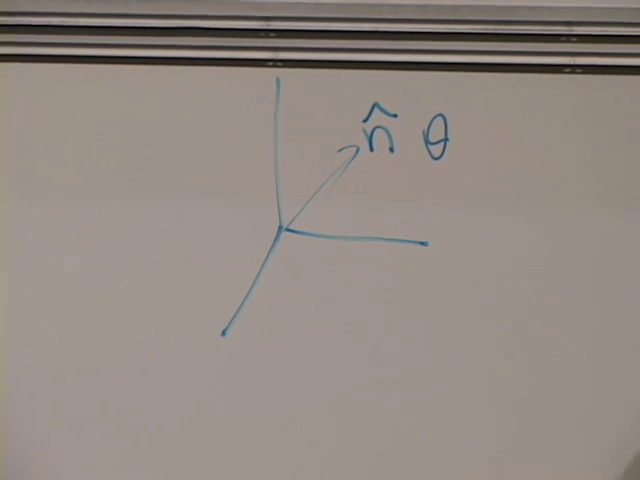
\includegraphics[width=0.58\textwidth]{lecture_03_figure_02.png}
\caption{Ось \(\hat{\boldsymbol n}\) и угол \(\theta\) задают пространственное вращение.}
\lectureframe{00:02:34}
\end{figure}

Направление на единичной сфере требует двух параметров, например долготы и широты. Угол поворота вокруг этого направления дает третий. Поэтому вращения образуют трехпараметрическое семейство. Мы пока не будем беспокоиться о глобальных отождествлениях, возникающих из-за углов, отличающихся на \(2\pi\); здесь важен именно локальный подсчет параметров.

Описание через ось и угол содержит некоторую избыточность. Если обратить ось и одновременно изменить знак угла, получится та же операция, а достаточно большие углы можно сводить по модулю полного оборота. Ничто из этого не меняет того факта, что вблизи единичного элемента вращение имеет три непрерывно изменяющихся параметра. Этот локальный счет позже будет сопоставлен с числом независимых параметров в матричном представлении.

Свойства группы теперь можно поочередно проверить:
\begin{enumerate}
\item \emph{Замкнутость.} Последовательное выполнение двух вращений дает другое вращение.
\item \emph{Единичный элемент.} Ничего не делать — это тождественное вращение.
\item \emph{Обратный элемент.} Вращение на \(\theta\) вокруг \(\hat{\boldsymbol n}\) компенсируется вращением на \(-\theta\) вокруг той же оси.
\item \emph{Ассоциативность.} Для трех последовательных вращений выполняется
\[
(R_1R_2)R_3=R_1(R_2R_3).
\]
\end{enumerate}

Вращения некоммутативны. Вращение вокруг оси \(x\), за которым следует вращение вокруг оси \(y\), вообще говоря, приводит к иной ориентации, чем те же две операции в обратном порядке:
\begin{equation}
R_x(\alpha)R_y(\beta)\ne R_y(\beta)R_x(\alpha).
\end{equation}
Различие становится величиной второго порядка, когда оба угла очень малы, поэтому бесконечно малые вращения могут казаться почти коммутативными. Тем не менее полная группа неабелева.

Некоммутативность можно проверить и без всяких уравнений. Возьмите книгу или коробку, отметьте одну грань как переднюю и поверните предмет на девяносто градусов вокруг оси \(x\), а затем на девяносто градусов вокруг оси \(y\). Верните его в исходную ориентацию и поменяйте порядок. Отмеченная грань окажется направленной иначе. Для малых углов расхождение заметить труднее, но оно не исчезло; оно начинается с произведения двух малых углов.

\begin{classroomqa}
\audiencequestion{Эти вращения последовательные, а не одновременные?\lecturetimestamp{00:04:45}}
\lecturerresponse{Да. Умножение в группе означает, что одна операция выполняется после другой. Именно порядок этих последовательных вращений может не коммутировать.}
\end{classroomqa}

Это наша первая неабелева группа. Ее дальнейшее применение связано не с цветом обычного предмета, а с красным, зеленым и синим цветовыми состояниями кварка. Это внутренняя система с тремя состояниями, и ее нетривиальные преобразования смешивают три цвета. Обычные вращения дают знакомую модель того, как непрерывная группа действует через матрицы.

Сама по себе группа абстрактна. Чтобы использовать ее в физике, надо указать, на каких объектах она действует. {Представление} сопоставляет каждому элементу группы оператор или матрицу так, что умножение элементов группы воспроизводится умножением сопоставленных матриц. Разные физические объекты могут нести разные представления одной и той же группы. Векторы, состояния со спином 1 и состояния со спином 1/2 дадут три примера.

\section{Трехмерное векторное представление}

Пусть обычный вектор имеет компоненты
\begin{equation}
\boldsymbol V=(V_x,V_y,V_z),\qquad V_i,\quad i=1,2,3.
\end{equation}
Можно вращать сам физический вектор, удерживая оси неподвижными, или вращать координатные оси, удерживая вектор неподвижным. Соглашения различаются, но в обоих описаниях компоненты смешиваются матрицей \(3\times3\). Для каждой пары ось–угол \((\hat{\boldsymbol n},\theta)\) запишем
\begin{equation}
V_i'=R_{ij}(\hat{\boldsymbol n},\theta)V_j,
\label{eq:l3-vector-rotation}
\end{equation}
где по повторяющемуся индексу производится суммирование.

Повторяющийся индекс \(j\) — фиктивный индекс. Уравнение~\eqref{eq:l3-vector-rotation} в явном виде означает
\begin{equation}
V_i'=R_{i1}V_1+R_{i2}V_2+R_{i3}V_3
\end{equation}
для каждой результирующей компоненты \(i\). Свободный индекс \(i\) указывает, какая компонента вычисляется; по повторяющемуся \(j\) ведется суммирование, и его можно переименовать, не меняя уравнения. Разделение этих двух ролей предотвращает большинство ошибок с индексами в рассуждении о сохранении длины.

\begin{figure}[htbp]
\centering
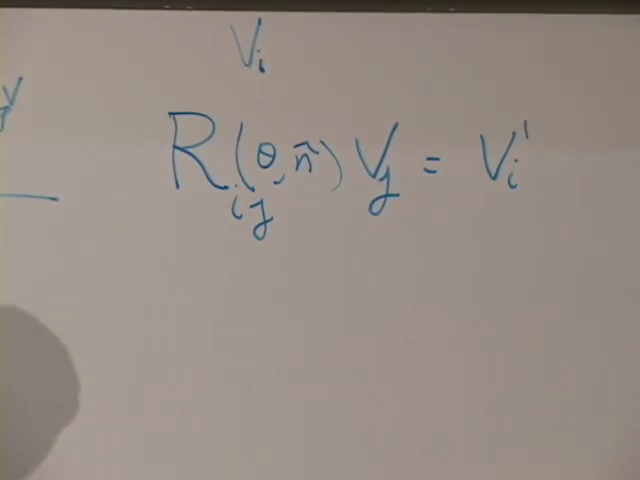
\includegraphics[width=0.68\textwidth]{lecture_03_figure_03.png}
\caption{Матрица вращения переводит исходные компоненты вектора в компоненты после поворота.}
\lectureframe{00:07:41}
\end{figure}

Настоящее вращение сохраняет длину. Пока и \(V_i\), и \(R_{ij}\) вещественны, поэтому
\begin{equation}
V_i'V_i'=V_iV_i
\end{equation}
для любого вектора. Чтобы выявить условие на матрицу, запишем то же преобразование с другими фиктивными индексами:
\begin{equation}
V_i'=R_{ij}V_j,\qquad V_i'=R_{ik}V_k.
\end{equation}
Перемножая и суммируя по \(i\), получаем
\begin{align}
V_i'V_i'
 &=R_{ij}V_jR_{ik}V_k\\
 &=R_{ij}R_{ik}V_jV_k.
\end{align}
Это равно \(V_jV_j\) при любом выборе \(V\) только в том случае, если
\begin{equation}
R_{ij}R_{ik}=\delta_{jk}.
\label{eq:l3-orthogonality-index}
\end{equation}
В матричной записи
\begin{equation}
R^TR=\boldsymbol 1,
\label{eq:l3-orthogonal}
\end{equation}
и, следовательно,
\begin{equation}
R^{-1}=R^T.
\end{equation}
Транспонирование просто меняет строки и столбцы местами.

Почему коэффициент должен быть равен \(\delta_{jk}\)? Символ Кронекера при суммировании полагает \(j=k\):
\begin{equation}
\delta_{jk}V_jV_k=V_1^2+V_2^2+V_3^2.
\end{equation}
Если бы \(R_{ij}R_{ik}\) отличалось от \(\delta_{jk}\), то длина менялась бы либо для некоторого направления, либо из-за некоторого перекрестного члена \(V_jV_k\). Поскольку равенство требуется для всякого возможного вектора, а не только для одного выбранного, сам этот матричный коэффициент должен совпадать с единичной матрицей.

Уравнение~\eqref{eq:l3-orthogonal} есть определяющее условие ортогональности для этого вещественного матричного представления. Умножение матриц воспроизводит таблицу умножения пространственных вращений. Это не единственное представление группы вращений; просто его легче всего наглядно представить.

Соотношение для обратной матрицы имеет непосредственный геометрический смысл. Вращение можно обратить, не решая нового матричного уравнения: достаточно поменять местами строки и столбцы. Если \(R_1\) и \(R_2\) представляют два вращения, то \(R_2R_1\) представляет их последовательное действие и снова является ортогональной матрицей. Тем самым матричные операции сохраняют ту же структуру замкнутости, единичного элемента, обратного элемента и ассоциативности, которая была установлена геометрически.

\section{Спин 1 и векторное представление}

Трехмерное представление действует и на квантовые состояния. У частицы со спином 1 возможны три проекции спина,
\begin{equation}
m=+1,\quad 0,\quad -1.
\end{equation}
Поэтому ее спиновое состояние представляет собой трехкомпонентный столбец амплитуд вероятности. Вращение частицы или изменение ориентации магнитного поля, используемого для задания оси спина, смешивает эти три амплитуды согласно трехмерному представлению группы вращений.

Число спиновых состояний подчиняется знакомому правилу \(2s+1\). Спин 0 имеет одно состояние, спин 1/2 — два, спин 1 — три, а спин 3/2 — четыре. Поэтому размерность вектора состояния зависит от спина. Одно и то же физическое вращение должно представляться матрицами разных размеров, когда оно действует в этих различных пространствах состояний.

Для частицы со спином 1 выберем базис
\begin{equation}
\lvert 1,+1\rangle,qquad
\lvert 1,0\rangle,qquad
\lvert 1,-1\rangle.
\end{equation}
Состояние имеет вид
\begin{equation}
\lvert\psi\rangle
=c_{+}\lvert1,+1\rangle+c_0\lvert1,0\rangle+c_{-}\lvert1,-1\rangle.
\end{equation}
Поворот установки не создает четвертого спинового состояния; он лишь смешивает между собой три коэффициента \(c_+,c_0,c_-\). Поэтому соответствующий оператор вращения должен быть матрицей \(3\times3\).

Для спина 1 это представление преобразуется так же, как обычный пространственный вектор. Именно в этом состоит точный смысл того, что частицу со спином 1 называют \emph{векторной частицей}: ее три спиновые амплитуды и три компоненты вектора подчиняются одному и тому же закону вращения. Квантовое состояние не нужно представлять как буквальную стрелку; утверждение относится к тому, как смешиваются его компоненты.

Это соответствие не случайно. Трёхвектор и состояние со спином 1 несут эквивалентные трёхмерные представления группы вращений. Слова emph{векторная частица} кратко выражают это свойство преобразования. Они не утверждают, что квантовое состояние поляризации — это крошечная жёсткая стрелка, скрытая внутри частицы.

\section{Дискретные и непрерывные симметрии}

Прежде чем перейти к спину 1/2, полезно различить два широких класса групп. Простое дискретное пример даёт отражение. Есть тождественный элемент и есть отражение \(P\); либо отражение происходит, либо нет. Напротив, фаза
\begin{equation}
e^{i\phi}
\end{equation}
непрерывно зависит от \(\phi\), а пространственное вращение непрерывно зависит от своей оси и угла. Такие непрерывные группы называются \emph{группами Ли}, в честь Софуса Ли; его фамилия произносится \emph{Ли}. Основное внимание будет уделено непрерывным симметриям, хотя дискретные симметрии также остаются важными.

Для двухэлементной группы отражений,
\begin{equation}
P^2=1.
\end{equation}
Между \(1\) и \(P\) нет непрерывно регулируемой степени отражения. С фазовой группой дело обстоит иначе: между \(e^{i\phi_1}\) и \(e^{i\phi_2}\) лежит непрерывное множество других фаз. Пространственные вращения обладают тем же непрерывным характером, но, в отличие от \(U(1)\), они неабелевы.

Спин 0 даёт простейшее представление группы вращений. Состояние со спином 0 не изменяется при любом вращении, поэтому каждый элемент группы представляется одномерной единицей:
\begin{equation}
D^{(0)}(R)=1.
\end{equation}
Сама группа по-прежнему содержит бесконечно много вращений; тривиальным является именно представление на состоянии со спином 0.

Это различие между группой и одним из её представлений существенно. Группа вращений не сводится к группе из одного элемента всякий раз, когда она действует на скаляр. Напротив, каждый её элемент на этом конкретном скалярном состоянии представляется одним и тем же числом \(1\).

\section{Общее состояние со спином 1/2}

Система со спином 1/2 имеет два базисных состояния. Относительно выбранной оси \(z\),
\begin{equation}
\lvert\uparrow\rangle=
\begin{pmatrix}1\\0\end{pmatrix},
\qquad
\lvert\downarrow\rangle=
\begin{pmatrix}0\\1\end{pmatrix}.
\end{equation}
Общее состояние есть двухкомпонентный спинор,
\begin{equation}
\lvert\psi\rangle=
\begin{pmatrix}\alpha_1\\\alpha_2\end{pmatrix},
\qquad
|\alpha_1|^2+|\alpha_2|^2=1.
\label{eq:l3-spinor}
\end{equation}
Его компоненты комплексны. Выбор \((\alpha_1,\alpha_2)=(1,0)\) соответствует спину вверх, а \((0,1)\) — спину вниз. Общая нормированная комбинация описывает спин, поляризованный вдоль некоторого другого направления.

Слова emph{вверх} и emph{вниз} имеют смысл только после выбора оси. Здесь этой осью является \(z\). Другой оси измерения соответствует другая пара базисных состояний, и состояние, которое вдоль одной оси определённо является верхним, в другом базисе, как правило, выглядит как суперпозиция. При вращении физического спина или при вращении осей отсчёта коэффициенты изменяются соответствующим образом.

Две комплексные амплитуды содержат 4 вещественных параметра. Нормировка устраняет один, а физически несущественная общая фаза устраняет ещё один, так что остаются два вещественных параметра. Это ровно то число, которое нужно, чтобы задать направление на сфере. Нам не нужно выводить явное соответствие между \((\alpha_1,\alpha_2)\) и этим направлением, чтобы изучать вращения.

Общая фаза устраняется, потому что
\begin{equation}
\begin{pmatrix}\alpha_1\\\alpha_2\end{pmatrix}
\quad\hbox{and}\quad
e^{i\chi}
\begin{pmatrix}\alpha_1\\\alpha_2\end{pmatrix}
\end{equation}
представляют один и тот же физический луч. Нормировка фиксирует полную вероятность, а не направление в обычном евклидовом пространстве. После обеих этих идентификаций оставшиеся два параметра можно рассматривать как полярный и азимутальный углы направления поляризации спина.

Когда спин вращается, его состояние становится
\begin{equation}
\alpha_i'=U_{ij}\alpha_j,
\qquad
\begin{pmatrix}\alpha_1'\\\alpha_2'\end{pmatrix}
=
\begin{pmatrix}
U_{11}&U_{12}\\
U_{21}&U_{22}
\end{pmatrix}
\begin{pmatrix}\alpha_1\\\alpha_2\end{pmatrix}.
\label{eq:l3-spinor-transform}
\end{equation}
Следовательно, пространственные вращения обладают двумерным матричным представлением, действующим на спиноры. В этом представлении имеется глобальная двузначность, обсуждение которой мы пока отложим; локально матрицы обладают свойствами преобразования, необходимыми далее.

Преобразованная пара \((\alpha_1',\alpha_2')\) снова должна быть допустимым квантовым состоянием. Поэтому первый вопрос о \(U\) — не его явная формула через ось и угол, а условие, при котором оно сохраняет нормировку любого исходного спинора.

\section{Сохранение вероятности и унитарные матрицы}

Вращение должно переводить нормированное состояние в другое нормированное состояние:
\begin{equation}
\alpha_i^*\alpha_i=\alpha_i'^*\alpha_i'=1.
\end{equation}
Подставляя уравнение~\eqref{eq:l3-spinor-transform},
\begin{align}
\alpha_i'^*\alpha_i'
 &=(U_{ij}\alpha_j)^*(U_{ik}\alpha_k)\\
 &=\alpha_j^*U_{ij}^*U_{ik}\alpha_k.
\end{align}
Поэтому аналог условия для вещественного вектора имеет вид
\begin{equation}
(U^T)^*U=\boldsymbol 1.
\end{equation}
Транспонирование с последующим комплексным сопряжением даёт эрмитово сопряжение,
\begin{equation}
U^\dagger=(U^T)^*,
\end{equation}
так что условие сохранения нормировки таково:
\begin{equation}
U^\dagger U=\boldsymbol 1.
\label{eq:l3-unitarity}
\end{equation}

Дополнительное комплексное сопряжение — единственное существенное изменение по сравнению с вычислением для вещественного вектора. Для вещественного вектора \(V_iV_i\) есть длина. Для спинора \(\alpha_i^*\alpha_i\) есть вероятность. Комплексное сопряжение необходимо, чтобы сделать эту вероятность вещественной и неотрицательной, поэтому транспонирование заменяется эрмитовым сопряжением.

Уравнение~\eqref{eq:l3-unitarity} также сразу даёт обратную матрицу:
\begin{equation}
U^{-1}=U^\dagger.
\end{equation}
Поэтому обратное вращение сохраняет ту же вероятностную норму. Как и для обычных матриц вращения, произведения унитарных матриц остаются унитарными, так что представление согласовано с групповым умножением.

\begin{figure}[htbp]
\centering
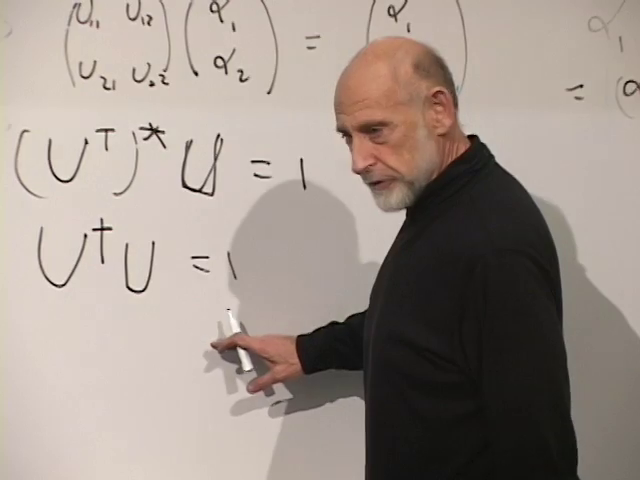
\includegraphics[width=0.62\textwidth]{lecture_03_figure_04.png}
\caption{Матрица вращения спинора удовлетворяет условию \(U^\dagger U=\boldsymbol 1\).}
\lectureframe{00:27:41}
\end{figure}

Матрицы, удовлетворяющие уравнению~\eqref{eq:l3-unitarity}, унитарны. Общая комплексная матрица \(2\times2\) содержит 8 вещественных параметров. Унитарность есть матричное уравнение \(2\times2\), дающее 4 независимых вещественных ограничения, так что остаются 4 параметра. Пространственное вращение имеет только 3. Нужно ещё одно ограничение, чтобы выделить спинорное представление вращений из всего \(U(2)\).

Эти 4 ограничения можно увидеть и иначе, если рассматривать два столбца \(U\) как два комплексных вектора. Каждый столбец должен иметь единичную норму, что даёт 2 вещественных условия, а столбцы должны быть ортогональны, что даёт одно комплексное, или 2 вещественных, условия. Итого получается 4. Оставшийся четвёртый параметр в \(U(2)\) окажется общей фазой детерминанта, а не новым пространственным вращением.

\section{Детерминант, равный единице, и \texorpdfstring{\(SU(2)\)}{SU(2)}}

Дополнительное условие таково:
\begin{equation}
\det U=1.
\label{eq:l3-det-one}
\end{equation}
Оно совместимо с групповым умножением, поскольку
\begin{equation}
\det(AB)=\det A\,\det B.
\end{equation}
Произведение двух унитарных матриц с детерминантом, равным 1, снова имеет детерминант 1, и единичная матрица имеет детерминант 1. Эти матрицы образуют замкнутую подгруппу.

Обратный элемент также принадлежит этой подгруппе. Если \(\det U=1\), то
\begin{equation}
\det U^{-1}=\frac{1}{\det U}=1.
\end{equation}
Следовательно, наложение условия det=1 не устраняет единичный элемент, не нарушает замкнутость и не лишает группу обратных элементов. Оно последовательно выделяет группу с одним непрерывным параметром меньше.

Сама по себе унитарность влечёт
\begin{equation}
\det(U^\dagger U)=
(\det U)^*\det U
=|\det U|^2=1.
\end{equation}
Она не вынуждает \(\det U\) быть равным \(+1\) или \(-1\). Детерминант общей унитарной матрицы может быть любой фазой:
\begin{equation}
\det U=e^{i\phi},
\qquad
\det U^\dagger=e^{-i\phi}.
\end{equation}
Условие~\eqref{eq:l3-det-one} фиксирует эту в противном случае свободную фазу и устраняет один вещественный параметр.

\begin{classroomqa}
\audiencequestion{Следует ли из \(U^\dagger U=\boldsymbol 1\), без условия единичного детерминанта, что \(\det U^\dagger\) должно равняться \(\det U\) или принимать только значения \(+1\) или \(-1\)?\lecturetimestamp{00:31:21}}
\lecturerresponse{Нет. Эти два детерминанта комплексно сопряжены. Они могут быть равны \(e^{i\phi}\) и \(e^{-i\phi}\), произведение которых равно единице. Ограничение специальной унитарности затем фиксирует оба равными единице.}
\end{classroomqa}

Унитарные матрицы \(n\times n\) образуют \(U(n)\). При \(n=1\) унитарная матрица — это просто фаза \(e^{i\phi}\), что даёт \(U(1)\). Подгруппа с детерминантом, равным 1, есть \emph{специальная унитарная группа},
\begin{equation}
SU(n)=\{U\in U(n):\det U=1\}.
\end{equation}
На двухкомпонентный спинор действует \(SU(2)\), группа с 3 параметрами.

Обозначение отражает оба ограничения: \(U\) означает унитарность, тогда как \(S\) означает, что группа специальная, то есть с детерминантом 1. Такие специальные унитарные группы возникают вновь и вновь, потому что они сохраняют комплексное внутреннее произведение, исключая при этом независимую общую фазу, связанную с детерминантом.

Локально \(SU(2)\) имеет ту же алгебру вращений и ту же структуру умножения, которые нужны для вращения состояний со спином 1/2. Глобально нужно помнить об отложенной тонкости: \(SU(2)\) является двукратным накрытием обычной группы вращений \(SO(3)\), так что двум элементам \(SU(2)\) соответствует одно пространственное вращение. \editorialnote{Формулировка через двукратное накрытие точно выражает упомянутую, но не развитую в исходном тексте, двузначность.}

\section{Бесконечно малые вращения и матрицы Паули}

\begin{classroomqa}
\audiencequestion{Где в этой конструкции появляются спиновые матрицы, или матрицы Паули?\lecturetimestamp{00:33:16}}
\lecturerresponse{Они появляются, когда элемент группы берётся очень близким к единице, что соответствует вращению на очень малый угол. Они являются генераторами этих бесконечно малых вращений.}
\end{classroomqa}

Начнём с
\begin{equation}
U=\boldsymbol 1+\epsilon M+O(\epsilon^2),
\label{eq:l3-small-u-anti}
\end{equation}
где \(\epsilon\) вещественно и мало. Тогда
\begin{equation}
U^\dagger=\boldsymbol 1+\epsilon M^\dagger+O(\epsilon^2),
\end{equation}
и из унитарности следует
\begin{align}
U^\dagger U
 &=\boldsymbol 1+\epsilon(M^\dagger+M)+O(\epsilon^2).
\end{align}
В первом порядке,
\begin{equation}
M^\dagger=-M.
\end{equation}
Следовательно, матрица \(M\) в уравнении~\eqref{eq:l3-small-u-anti} антиэрмитова.

Сохраняются только члены, линейные по \(\epsilon\). Произведение \(\epsilon^2M^\dagger M\) отбрасывается, потому что оно имеет второй порядок. В этом и состоит преимущество работы вблизи единицы: нелинейные групповые условия превращаются в линейные условия на их генераторы.

Удобнее вынести множитель \(i\):
\begin{equation}
U=\boldsymbol 1+i\epsilon H+O(\epsilon^2).
\label{eq:l3-small-u-herm}
\end{equation}
При комплексном сопряжении \(i\) переходит в \(-i\), поэтому
\begin{equation}
U^\dagger=\boldsymbol 1-i\epsilon H^\dagger+O(\epsilon^2).
\end{equation}
Теперь
\begin{equation}
U^\dagger U
=\boldsymbol 1+i\epsilon(H-H^\dagger)+O(\epsilon^2),
\end{equation}
и унитарность в первом порядке требует
\begin{equation}
H^\dagger=H.
\end{equation}
Когда множитель \(i\) вынесен явно, генератор является эрмитовым.

Умножение на \(i\) не изменило допустимые бесконечно малые матрицы; оно лишь изменило соглашение, по которому называют генератор. В физике обычно выбирают эрмитовы генераторы, потому что их собственные значения вещественны и потому что соответствующие наблюдаемые, такие как момент импульса, эрмитовы.

Условие равенства определителя единице даёт бесследовость\editorialnote{В устном разложении определителя индексы на короткое время искажены. Исправленный линейный член — \(A_{11}+A_{22}=\operatorname{tr}A\); произведения внедиагональных элементов начинаются со второго порядка.}. Для малой матрицы \(2\times2\) \(A\),
\begin{equation}
\det(\boldsymbol 1+A)
=
\det
\begin{pmatrix}
1+A_{11}&A_{12}\\
A_{21}&1+A_{22}
\end{pmatrix}.
\end{equation}
Раскрывая определитель,
\begin{align}
\det(\boldsymbol 1+A)
 &=(1+A_{11})(1+A_{22})-A_{12}A_{21}\\
 &=1+A_{11}+A_{22}+O(A^2)\\
 &=1+\operatorname{tr}A+O(A^2).
\end{align}
Применяя это к \(A=i\epsilon H\),
\begin{equation}
\det U=1+i\epsilon\,\operatorname{tr}H+O(\epsilon^2).
\end{equation}
Следовательно, \(\det U=1\) требует
\begin{equation}
\operatorname{tr}H=0.
\end{equation}
Условие на след устраняет в точности генератор, пропорциональный единичной матрице. Общая эрмитова матрица \(2\times2\) имеет четыре вещественных параметра: два вещественных диагональных элемента и один комплексный внедиагональный элемент. Её след фиксирует одну вещественную комбинацию, оставляя три. Это соответствует трём осям, относительно которых можно совершить бесконечно малый пространственный поворот.

Таким образом, бесконечно малые генераторы \(SU(2)\) — это бесследовые эрмитовы матрицы \(2\times2\). Три матрицы Паули образуют базис:
\begin{equation}
\begin{aligned}
\sigma_x&=
\begin{pmatrix}0&1\\1&0\end{pmatrix},
&
\sigma_y&=
\begin{pmatrix}0&-i\\i&0\end{pmatrix},
\\[0.4em]
\sigma_z&=
\begin{pmatrix}1&0\\0&-1\end{pmatrix}.
\end{aligned}
\end{equation}
Любой генератор можно записать в виде
\begin{equation}
H=a_x\sigma_x+a_y\sigma_y+a_z\sigma_z.
\end{equation}
Малый поворот вокруг оси \(x\) выделяет \(\sigma_x\); поворот вокруг оси \(y\) — \(\sigma_y\); а поворот вокруг любой другой оси выделяет соответствующую линейную комбинацию. В единицах, где \(\hbar=1\), операторы спина имеют вид
\begin{equation}
S_i=\frac{\sigma_i}{2}.
\end{equation}

Например, оси, лежащей посередине между \(x\) и \(y\), соответствует генератор, пропорциональный
\begin{equation}
\frac{\sigma_x+\sigma_y}{\sqrt2}.
\end{equation}
Направление вектора коэффициентов \((a_x,a_y,a_z)\) задаёт ось поворота, тогда как его модуль вместе с \(\epsilon\) задаёт малый угол. В этом и состоит связь между спиновыми матрицами, встречающимися в коммутационных соотношениях для момента импульса, и операторами конечных поворотов. В частности,
\begin{equation}
[S_x,S_y]=iS_z
\end{equation}
а её циклические аналоги кодируют некоммутативность, уже увиденную геометрически. Стандартный конечный поворот получается экспоненцированием бесконечно малого генератора\editorialnote{Экспоненциальная формула конечного поворота представляет собой стандартное завершение бесконечно малого построения; в источнике выводятся только условия на генераторы и их базис из матриц Паули.},
\begin{equation}
U(\hat{\boldsymbol n},\theta)
=\exp\left(-\frac{i\theta}{2}\,
\hat{\boldsymbol n}\cdot\boldsymbol\sigma\right).
\end{equation}
\section{Трёхсостоянийное цветовое пространство}

Объединение представлений может подождать. Теперь мы оставим пространственный спин и вернёмся к цвету кварка. Кварк по-прежнему имеет спин 1/2, но его цвет — это независимая трёхсостоянийная степень свободы:
\begin{equation}
\lvert r\rangle,\qquad
\lvert g\rangle,\qquad
\lvert b\rangle.
\end{equation}
Общее цветовое состояние имеет вид
\begin{equation}
\begin{aligned}
\lvert q\rangle_{\mathrm{color}}
={}&
\alpha_r\lvert r\rangle
+\alpha_g\lvert g\rangle
+\alpha_b\lvert b\rangle,
\\
&|\alpha_r|^2+|\alpha_g|^2+|\alpha_b|^2=1.
\end{aligned}
\end{equation}
Эквивалентно,
\begin{equation}
q=
\begin{pmatrix}
\alpha_r\\
\alpha_g\\
\alpha_b
\end{pmatrix}.
\end{equation}
Квадраты модулей дают вероятности красного, зелёного и синего в выбранном цветовом базисе. Та же тройственная запись может объединить три оператора кваркового поля,
\begin{equation}
\psi=
\begin{pmatrix}
\psi_r\\
\psi_g\\
\psi_b
\end{pmatrix}.
\end{equation}

Спин и цвет нужно концептуально держать раздельно. Спиновая метка говорит нам, как состояние преобразуется при поворотах физического пространства. Цветовая метка говорит, как оно преобразуется при внутренней симметрии, которая не вращает лабораторию. Состояние кварка несёт обе метки, хотя в настоящем обсуждении спин опущен, чтобы сосредоточиться на цвете.

Запись трёх полевых операторов в одном столбце — это больше, чем просто удобство учёта. Она позволяет сформулировать симметрию одним матричным уравнением. Преобразование может превратить красный полевой оператор в линейную комбинацию красного, зелёного и синего полевых операторов, подобно тому как пространственный поворот превращает одну компоненту вектора в линейную комбинацию других компонент.

Сначала можно представить себе дискретные преобразования, которые обменивают два цвета. Более широкая симметрия содержит непрерывные смеси всех трёх. Простой матрице перестановки может понадобиться сопутствующая фаза, чтобы её определитель стал равен единице; тогда этот обмен оказывается вложенным в специальную унитарную группу.

Для двух базисных состояний сама по себе перестановка представляется как
\begin{equation}
X=
\begin{pmatrix}0&1\\1&0\end{pmatrix},
\qquad
\det X=-1.
\end{equation}
Умножение всей матрицы на \(i\) даёт
\begin{equation}
\det(iX)=i^2\det X=1.
\end{equation}
Следовательно, дискретный обмен может появляться как частный элемент большей непрерывной группы, если фаза выбрана согласованно.

\begin{classroomqa}
\audiencequestion{Разве у матрицы, которая просто переставляет два базисных состояния, не тот определитель, который нужен для \(SU(2)\)?\lecturetimestamp{00:43:46}}
\lecturerresponse{У самой перестановки определитель \(-1\). Подходящий множитель \(i\) даёт представителя с единичным определителем, так что этот обмен можно включить в непрерывные специальные унитарные преобразования.}
\end{classroomqa}

\section{\texorpdfstring{\(SU(3)\)}{SU(3)} и восемь цветовых генераторов}

Непрерывное цветовое преобразование имеет вид
\begin{equation}
\begin{aligned}
q'&=Uq,
&
U^\dagger U&=\boldsymbol 1,
\\
\det U&=1,
&
U&\in SU(3).
\end{aligned}
\label{eq:l3-su3-action}
\end{equation}
Математика здесь та же специальная унитарная конструкция, что используется для спиноров, но теперь \(U\) имеет размер \(3\times3\). Это не поворот физического пространства. Это поворот во внутреннем цветовом пространстве.

Унитарность сохраняет нормировку цветового состояния:
\begin{equation}
q^\dagger q
=|\alpha_r|^2+|\alpha_g|^2+|\alpha_b|^2.
\end{equation}
Условие равенства определителя единице устраняет из непрерывного смешивания общее фазовое направление \(U(1)\). Получающиеся матрицы могут осуществлять простые перестановки, относительные изменения фаз и подлинно непрерывные суперпозиции, оставаясь при этом в одной замкнутой группе.

Подсчёт параметров здесь непосредственен. Комплексная матрица \(3\times3\) имеет девять комплексных элементов, то есть восемнадцать вещественных параметров. Матричное уравнение \(U^\dagger U=\boldsymbol 1\) накладывает девять вещественных условий. Определитель, равный единице, убирает ещё один:
\begin{equation}
\dim SU(3)=18-9-1=8.
\end{equation}
Следовательно, \(SU(3)\) имеет восемь независимых бесконечно малых генераторов.

Девять вещественных условий унитарности можно снова понять через столбцы \(U\). Каждый из трёх комплексных столбцов должен иметь единичную норму, и каждая пара должна быть ортогональна. Эти условия устраняют девять из исходных восемнадцати вещественных параметров. Условие на фазу определителя устраняет десятый, оставляя восемь. Это трёхсостоянийный аналог подсчёта \(8-4-1=3\) для \(SU(2)\).

Появление числа восемь — это тот же самый факт, который в конечном счёте приводит к восьми видам глюонов. Утверждение, что глюонов не девять, потому что ограничение на определитель убрало одно направление, — лишь мнемоническая подсказка. Точнее, девять матриц цвет–антицвет разлагаются на одно цветосинглетное направление, пропорциональное единичной матрице, и восемь бесследовых направлений. Эти восемь бесследовых генераторов образуют присоединённую цветовую структуру, которую несут глюоны КХД.\editorialnote{Формулировка через синглет и октет — это стандартная точная версия намеренно эвристического замечания источника о детерминанте; построение калибровочного поля отложено.}

На этом этапе связь с восемью глюонами — это ориентир, а не полный вывод. Чтобы получить калибровочные частицы, нужно повысить цветовую симметрию до локальной и определить компенсирующие поля. Подсчёт параметров уже показал, что существуют восемь независимых направлений, в которых цветовое преобразование \(SU(3)\) может начать отклоняться от тождественного.

\section{Цветовая симметрия накладывает ограничения на КХД}

Основное утверждение о симметрии состоит в том, что физика инвариантна относительно цветового преобразования из уравнения~\eqref{eq:l3-su3-action}. Это центральная внутренняя симметрия квантовой хромодинамики. Смешивание цветовых компонент по форме аналогично смешиванию амплитуд спина вверх и спина вниз, а эти спинорные преобразования, в свою очередь, связаны с поворотами пространственных направлений, но эти три пространства нельзя путать.

Называть цвет симметрией значит утверждать, что смена цветового базиса не меняет физических предсказаний. Красный, зелёный и синий — это удобные названия для трёх базисных векторов, а не трёх наблюдаемых пигментов. Одновременный поворот цветовых компонент по \(SU(3)\) должен оставлять вид законов неизменным. Эта инвариантность — не факультативная эстетическая черта; это организующий принцип КХД.

Симметрия ограничивает лагранжиан. В более раннем примере с \(U(1)\) инвариантность относительно общего фазового преобразования накладывала условие, чтобы допустимые члены содержали сбалансированные множители поля и его сопряжения. В КХД каждый член также должен быть инвариантен относительно цветового преобразования \(SU(3)\). Это требование имеет последствия для взаимодействий, сохраняющихся величин и вида глюонного поля.

Предположим, что некоторый предложенный член содержит незакрытый цветовой индекс. При действии уравнения~\eqref{eq:l3-su3-action} этот индекс преобразуется, так что такой член сам по себе не может быть инвариантным. Допустимые члены должны свёртывать цветовые индексы в инвариантные комбинации или использовать калибровочные поля, преобразования которых компенсируют это изменение. В этом и состоит практическая сила принципа симметрии: он исключает произвольные взаимодействия и упорядочивает те, которые остаются.

Полное построение КХД требует ещё одного шага: нужно допустить, чтобы цветовое преобразование менялось от точки к точке, а калибровочное поле должно компенсировать это локальное изменение.\editorialnote{Локализация цветовой симметрии — это стандартное калибровочно-теоретическое завершение обсуждения глобального \(SU(3)\); в данной лекции это не излагается.} Его изложение относится к следующему этапу. На данный момент существенная структура уже задана: цветовой триплет, на который действует специальная унитарная симметрия трёх состояний с восемью генераторами.

Расчёт продвинулся в теорию групп настолько, насколько это сейчас необходимо. Мы начали с вращений, которые можно изобразить в обычном пространстве, перешли к матрицам, действующим на векторы и спиноры, а затем вновь применили ту же логику во внутреннем цветовом пространстве. Следующий шаг позволяет вернуться к физике частиц, когда необходимый математический аппарат уже имеется, вместо того чтобы требовать от формализма сразу нести на себе всё физическое содержание.
\chapter{Цветовые представления, адроны и конфайнмент}

\paragraph{Короткое вступительное отступление.}
Прежде чем вернуться к теории групп, позвольте одну бесстыдную рекламу. \emph{The Black Hole War} рассказывает историю долгого спора со Стивеном Хокингом о том, уничтожают ли черные дыры квантовую информацию. В ней также зафиксирована некоторая жестокость, свойственная теоретическим физикам: не только кот Шрёдингера, но и рыбки Сасскинда с их прискорбным путешествием в унитаз. Исполнив этот долг, вернемся к Алисе и Бобу. Алиса по-прежнему страдает, потому что Боб по-прежнему заставляет ее учить теорию групп.

\lectureoverview{Симметрия становится физической благодаря своему действию на состояния. Мы начнем с вращений, чтобы ввести представления и генераторы, а затем повторим это построение для цветовой группы \(SU(3)\). Цветовые представления объединяются в адроны, а их динамика объясняет, почему изолированный цвет никогда не наблюдается.}

\section{Группа и объекты, на которые она действует}

В любом обсуждении симметрии присутствуют две идеи. Во-первых, есть абстрактная группа: совокупность операций с законом умножения, единичным элементом и обратными элементами. Во-вторых, есть объекты, на которые эти операции действуют. Эти две идеи можно различать, но в физике их нельзя разделить. Симметрия важна потому, что она преобразует физические состояния, поля, координаты или наблюдаемые.

\begin{classroomqa}
\audiencequestion{Группа была описана и как абстрактная таблица умножения, и как матрицы, действующие на физические объекты. Можно ли отделить эти две части друг от друга?\lecturetimestamp{00:01:58}}
\lecturerresponse{Это разные уровни описания, но они полностью взаимосвязаны. Вращение существует как абстрактная операция еще до того, как мы укажем, что именно оно вращает. Затем физика спрашивает, как эта же операция действует на состояния и величины, относящиеся к данной системе. Матрицы задают это конкретное действие, сохраняя при этом абстрактный закон умножения.}
\end{classroomqa}

Пространственные вращения дают самый наглядный пример. Классически одно и то же вращение может действовать на координаты частицы, на направление магнита или на любой другой вектор. В квантовой механике состояния живут в линейном векторном пространстве, поэтому вращение представляется линейным оператором в этом пространстве. Если \(g\) обозначает абстрактный элемент группы, а \(D(g)\) — его матричный представитель, то согласованность означает
\begin{equation}
D(g_1g_2)=D(g_1)D(g_2),
\qquad
D(e)=\boldsymbol 1.
\end{equation}
Матрицы не обязаны быть похожи на абстрактные операции, но их умножение должно воспроизводить групповое умножение.
\editorialnote{Уравнение гомоморфизма явно записывает соответствие между групповым умножением и умножением матриц, которое в исходном тексте описано словами.}

Размерность матрицы определяется пространством состояний, а не одной только абстрактной группой. Если мы оставляем только спин одного электрона, то существуют две ортогональные возможности — спин вверх и спин вниз, — и состояние представляет собой двухкомпонентный столбец. Поэтому вращения действуют через матрицы \(2\times2\). Для двух объектов со спином 1/2 существуют четыре базисных состояния,
\begin{equation}
\ket{\uparrow\uparrow},\qquad
\ket{\uparrow\downarrow},\qquad
\ket{\downarrow\uparrow},\qquad
\ket{\downarrow\downarrow},
\end{equation}
и соответствующее действие на объединенном пространстве четырехмерно.

Хорошо знакомая последовательность такова
\begin{equation}
\begin{array}{c|c|c}
\text{spin} & \text{number of states} & \text{matrix dimension}\\
\hline
0 & 1 & 1\times1\\
\frac12 & 2 & 2\times2\\
1 & 3 & 3\times3\\
\frac32 & 4 & 4\times4
\end{array}
\end{equation}
и так далее. Состояние со спином нуль реализует тривиальное представление: любое вращение оставляет его неизменным. Матрица размерности один на один — это просто \(1\). Состояние со спином 1 имеет три компоненты, и его матрицы вращения — это обычные трехмерные векторные вращения. В более общем случае спин \(j\) имеет \(2j+1\) состояний.

Представление может быть и бесконечномерным. Если мы описываем полное орбитальное движение электрона, а не только его спин, то состояние содержит амплитуду для каждого положения или, эквивалентно, для каждого импульса. Тогда оператор вращения действует на бесконечномерном пространстве волновых функций. Таким образом, одна и та же абстрактная группа вращений имеет тривиальные, двумерные, трехмерные и бесконечномерные представления. Именно этот факт мы снова используем, когда обсуждение перейдет от спина к цвету.

\section{Почему спиновые вращения являются специальными унитарными преобразованиями}

Теперь вернемся к спину одного электрона и отбросим его орбитальное движение. Вращение представляется унитарной матрицей \(U\) размера \(2\times2\),
\begin{equation}
U^\dagger U=\boldsymbol 1,
\qquad
U^{-1}=U^\dagger.
\label{eq:l4-unitarity}
\end{equation}
Обратное преобразование должно отменять вращение, а унитарность сохраняет норму и, следовательно, любую вероятность.

Общая комплексная матрица размера \(2\times2\) содержит четыре комплексных элемента, то есть 8 вещественных параметров. Уравнение~\eqref{eq:l4-unitarity} накладывает 4 независимых вещественных условия, оставляя 4 параметра. Обычное пространственное вращение имеет только 3: два параметра задают ось и один задает угол. Поэтому унитарная матрица содержит одну лишнюю фазу. Дополнительное ограничение имеет вид
\begin{equation}
\det U=1.
\label{eq:l4-det-one}
\end{equation}
Тогда подсчет дает
\begin{equation}
8-4-1=3.
\end{equation}

Ограничение на единичный детерминант устойчиво относительно умножения, поскольку
\begin{equation}
\det(AB)=\det A\,\det B.
\end{equation}
Если каждая из двух матриц имеет детерминант 1, то то же верно и для их произведения. Оно также совместимо с унитарностью. Взяв детерминант от уравнения~\eqref{eq:l4-unitarity}, получаем
\begin{equation}
1=\det(U^\dagger U)
=\det(U^\dagger)\det U
=(\det U)^*\det U.
\end{equation}
Следовательно, детерминант унитарной матрицы лежит на единичной окружности,
\begin{equation}
\det U=e^{i\phi}.
\end{equation}

\begin{classroomqa}
\audiencequestion{Требует ли унитарность, чтобы детерминант был вещественным?\lecturetimestamp{00:12:10}}
\lecturerresponse{Нет. Унитарность требует только единичного модуля. Детерминант может быть любой чистой фазой \(e^{i\phi}\). Для двумерной матрицы умножение \(U\) на \(e^{-i\phi/2}\) устраняет эту общую фазу и дает матрицу с детерминантом 1.}
\end{classroomqa}

Действительно, если
\begin{equation}
V=e^{-i\phi/2}U,
\end{equation}
то \(V\) остается унитарной, и
\begin{equation}
\det V=e^{-i\phi}\det U=1.
\end{equation}
Унитарные матрицы с детерминантом 1 образуют \(SU(2)\).

Здесь есть одна тонкость. Возникает соблазн сказать, что \(SU(2)\) — это просто группа вращений в трехмерном пространстве, но соответствие здесь два к одному. Матрицы \(U\) и \(-U\) по-разному действуют на спинор, однако соответствуют одному и тому же вращению обычного вектора. Таким образом,
\begin{equation}
SU(2)/\{\boldsymbol 1,-\boldsymbol 1\}\simeq SO(3).
\end{equation}
Для настоящего обсуждения важны локальная структура умножения и три генератора, но двулистное накрытие объясняет двузначность вращений спина 1/2.

\section{Бесконечно малые преобразования и их генераторы}

Конечное вращение можно составить из множества очень малых вращений. Элемент группы, близкий к единичному, называется бесконечно малым, и знания всех бесконечно малых направлений достаточно, чтобы в связной группе восстановить конечные преобразования повторным умножением. Еще важнее для физики то, что операторы, порождающие эти бесконечно малые преобразования, являются сохраняющимися величинами, связанными с этой симметрией.

Запишем элемент, близкий к единице, в виде
\begin{equation}
U=\boldsymbol 1+i\epsilon T,
\qquad |\epsilon|\ll1.
\label{eq:l4-infinitesimal-u}
\end{equation}
Множитель \(i\) — удобное соглашение. Подстановка в условие унитарности и отбрасывание членов порядка \(\epsilon^2\) дает
\begin{align}
(\boldsymbol 1+i\epsilon T)
(\boldsymbol 1-i\epsilon T^\dagger)&=\boldsymbol 1,
\\
i\epsilon(T-T^\dagger)&=0,
\\
T&=T^\dagger.
\label{eq:l4-hermitian-generator}
\end{align}
Генератор эрмитов, как и должно быть для квантовомеханической наблюдаемой.

\begin{figure}[htbp]
\centering
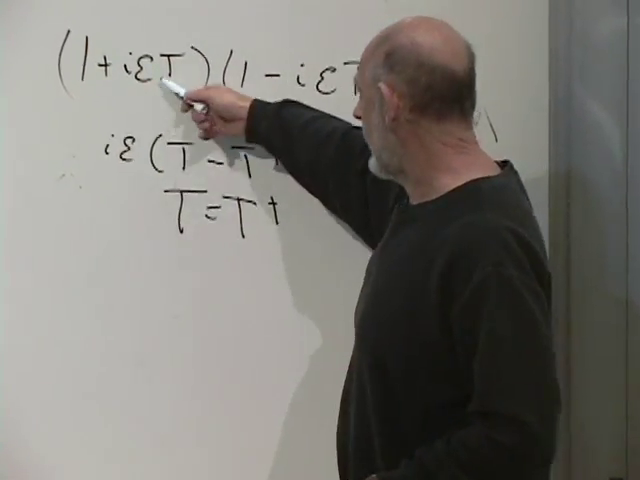
\includegraphics[width=0.62\textwidth]{lecture_04_figure_03.png}
\caption{Вычисление унитарности для элемента, близкого к единице, приводящее к \(T=T^\dagger\).}
\lectureframe{00:23:28}
\end{figure}

Для пространственных вращений существуют три линейно независимых генератора, потому что имеются три независимые бесконечно малые оси вращения. Малое вращение вокруг произвольной оси составляется из малых вращений вокруг \(x\), \(y\) и \(z\). Соответствующие генераторы — это операторы момента импульса \(J_x,J_y,J_z\). Их коммутаторы кодируют некоммутативность вращений,
\begin{equation}
[J_i,J_j]=i\epsilon_{ijk}J_k.
\label{eq:l4-angular-momentum-algebra}
\end{equation}
и из повторных бесконечно малых вращений затем строится конечное вращение.

Мы использовали унитарность, но еще не использовали условие единичного детерминанта. Для любой малой матрицы \(m\),
\begin{equation}
\det(\boldsymbol 1+\epsilon m)
=1+\epsilon\,\operatorname{tr}m+O(\epsilon^2).
\label{eq:l4-det-expansion}
\end{equation}

\begin{figure}[htbp]
\centering
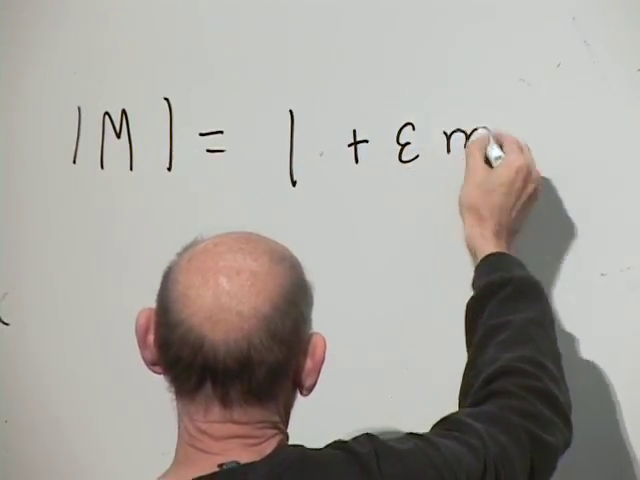
\includegraphics[width=0.62\textwidth]{lecture_04_figure_02.png}
\caption{Разложение детерминанта по первому порядку в том виде, в каком оно начинается на доске.}
\lectureframe{00:21:51}
\end{figure}

Применяя уравнение~\eqref{eq:l4-det-expansion} к уравнению~\eqref{eq:l4-infinitesimal-u},
\begin{equation}
\det U
=1+i\epsilon\,\operatorname{tr}T+O(\epsilon^2).
\end{equation}
Следовательно, условие специальной унитарности требует
\begin{equation}
\operatorname{tr}T=0.
\label{eq:l4-traceless-generator}
\end{equation}
Генераторы \(SU(2)\) — это в точности бесследовые эрмитовы матрицы \(2\times2\). Это векторное пространство имеет размерность 3. Стандартный базис задается матрицами Паули,
\begin{equation}
\begin{aligned}
\sigma_x&=
\begin{pmatrix}0&1\\1&0\end{pmatrix},
&
\sigma_y&=
\begin{pmatrix}0&-i\\i&0\end{pmatrix},
\\[0.4em]
\sigma_z&=
\begin{pmatrix}1&0\\0&-1\end{pmatrix}.
\end{aligned}
\end{equation}
Для представления со спином 1/2 можно взять \(J_i=\sigma_i/2\), так что конечное вращение на угол \(\theta\) вокруг \(\hat{\boldsymbol n}\) имеет вид
\begin{equation}
U(\hat{\boldsymbol n},\theta)
=\exp\!\left(-i\theta\,
\hat{\boldsymbol n}\cdot\boldsymbol\sigma/2\right).
\end{equation}
\editorialnote{Конечная экспонента является стандартным завершением обсуждения бесконечно малых генераторов. В исходном тексте подчеркиваются повторные малые вращения, а не явная запись этой формулы.}

\begin{classroomqa}
\audiencequestion{Итак, существуют три независимые бесследовые эрмитовы матрицы \(2\times2\)?\lecturetimestamp{00:24:07}}
\lecturerresponse{Да. Это три матрицы Паули. Для специальных унитарных матриц \(3\times3\) соответствующее число равно 8, и стандартный базис задается восемью матрицами Гелл-Манна.}
\end{classroomqa}

\begin{classroomqa}
\audiencequestion{Это та самая ``восьмёрка'', что и в восьмеричном пути и у восьми глюонов?
\lecturetimestamp{00:24:43}}
\lecturerresponse{Математика здесь — один и тот же тип теории представлений \(SU(3)\), но нужно указать, какая именно симметрия \(SU(3)\) действует. Историческая вкусовая симметрия восьмеричного пути — не цветовая \(SU(3)\). Восемь глюонов принадлежат присоединённому представлению цветовой \(SU(3)\).}
\end{classroomqa}

\section{От SU(2) к цветовой SU(3)}

Теперь увеличим матрицы с \(2\times2\) до \(3\times3\). Общая комплексная
\(3\times3\)-матрица имеет девять комплексных элементов, а значит, 18 вещественных параметров.
Условие \(U^\dagger U=\boldsymbol 1\) даёт 9 вещественных ограничений,
а \(\det U=1\) устраняет ещё одно. Поэтому
\begin{equation}
18-9-1=8.
\end{equation}
Имеются 8 независимых бесконечно малых направлений и 8 бесследовых
эрмитовых генераторов. В отличие от \(SU(2)\), эта группа не является группой вращений
обычного трёхмерного пространства. Это внутренняя симметрия, действующая на
цвет.

Прежде чем приписывать эти представления кваркам, вспомним, как возникают составные
представления. Соединим две системы со спином одна вторая и пренебрежём
их орбитальным движением. Получаются 4 состояния произведения, но вращение не перемешивает все 4 в одно неприводимое представление. Три комбинации преобразуются как спин 1,
\begin{align}
\ket{1,1}&=\ket{\uparrow\uparrow},\\
\ket{1,0}&=\frac{1}{\sqrt2}
(\ket{\uparrow\downarrow}+\ket{\downarrow\uparrow}),\\
\ket{1,-1}&=\ket{\downarrow\downarrow},
\end{align}
тогда как четвёртая преобразуется как спин 0,
\begin{equation}
\ket{0,0}=\frac{1}{\sqrt2}
(\ket{\uparrow\downarrow}-\ket{\downarrow\uparrow}).
\end{equation}
Следовательно,
\begin{equation}
\boldsymbol 2\otimes\boldsymbol 2
=\boldsymbol 3\oplus\boldsymbol 1.
\label{eq:l4-two-spin-decomposition}
\end{equation}
Состояния с сонаправленными спинами дают члены триплета с \(m=\pm1\), симметричное
состояние с нулевой проекцией завершает его, а антисимметричная комбинация является
синглетом. Именно такова общая логика сложения угловых моментов и объединения
цветовых представлений.

То же различие синглет--триплет возникает всякий раз, когда связываются две степени свободы
со спином одна вторая. В атомарном водороде спины электрона и протона
образуют сверхтонкие синглетное и триплетное состояния. В орто- и параводороде
та же теория представлений описывает ядерные спины двух протонов в молекуле
\(H_2\).
\editorialnote{В исходном тексте выражение ``орто- и параводород'' употребляется при обсуждении спинов в системе протон--электрон в атоме водорода. Математическое разложение верно; для точности здесь различаются молекулярные и атомные названия.}

\subsection{Триплет и антитриплет}

У отдельного кварка есть три цветовые амплитуды. В выбранном базисе запишем
\begin{equation}
q=
\begin{pmatrix}
q_r\\q_g\\q_b
\end{pmatrix},
\qquad
q'=Uq,
\qquad U\in SU(3).
\label{eq:l4-quark-triplet}
\end{equation}
Эти три компоненты могут быть амплитудами состояния одного кварка или тремя
операторами поля, создающими красный, зелёный и синий кварки. Группа перемешивает
три компоненты. Состояние, которое первоначально было красным, после цветового преобразования
вообще говоря становится суперпозицией красного, зелёного и синего. Это фундаментальное
трёхмерное представление называется \(\boldsymbol 3\).

Для антикварка группа действует через комплексно-сопряжённое к кварковому
представление. Взяв комплексное сопряжение уравнения~\eqref{eq:l4-quark-triplet}, получаем
\begin{equation}
\bar q'=U^*\bar q.
\end{equation}
Это представление обозначается \(\bar{\boldsymbol 3}\). Аналогия с \(U(1)\)
непосредственна: если электронное поле приобретает \(e^{i\theta}\), то позитронное поле
приобретает \(e^{-i\theta}\). Цветовые преобразования кварка и антикварка —
неабелева версия такого сопряжённого соответствия.

В окрестности единицы, если
\begin{equation}
U=\boldsymbol 1+i\epsilon T,
\end{equation}
то
\begin{equation}
U^*=\boldsymbol 1-i\epsilon T^*.
\end{equation}
Следовательно, генераторы антитриплета равны \(-T^*\), то есть это сопряжённые генераторы с противоположным
знаком. Именно в этом точном смысле антикварки несут противоположные цветовые
заряды.

\begin{classroomqa}
\audiencequestion{Что происходит с комплексно-сопряжённым представлением в случае \(SU(2)\)?
\lecturetimestamp{00:36:19}}
\lecturerresponse{Дублет \(SU(2)\) — особый случай: его комплексно-сопряжённое представление эквивалентно исходному дублету после фиксированной замены базиса с участием антисимметричного тензора эпсилон. Для \(SU(3)\) представления \(\boldsymbol 3\) и \(\bar{\boldsymbol 3}\) действительно неэквивалентны.}
\end{classroomqa}
\editorialnote{Математически точный термин для фундаментального представления \(SU(2)\) — псевдовещественное, а не вещественное. В ответе сохраняется задуманное в источнике различие, при этом терминология исправлена.}

\section{Комбинирование цветовых представлений}

Символ \(\otimes\) не означает обычного умножения чисел, написанных рядом с ним. Он означает, что объединяются два пространства состояний. Получающееся пространство тензорного произведения затем разлагается на части, которые под действием группы не смешиваются друг с другом.

\subsection{Два кварка: \texorpdfstring{\(\boldsymbol 3\otimes\boldsymbol 3\)}{3 x 3}}

У двух кварков есть 9 базисных цветовых состояний: красный--красный, красный--зелёный, красный--синий и остальные 6 упорядоченных пар. Разложим два цветовых индекса на симметричную и антисимметричную части. Симметричная часть имеет 6 независимых компонент; антисимметричная — 3. При \(SU(3)\),
\begin{equation}
\boldsymbol 3\otimes\boldsymbol 3
=\boldsymbol 6\oplus\bar{\boldsymbol 3}.
\label{eq:l4-three-times-three}
\end{equation}

\begin{figure}[htbp]
\centering
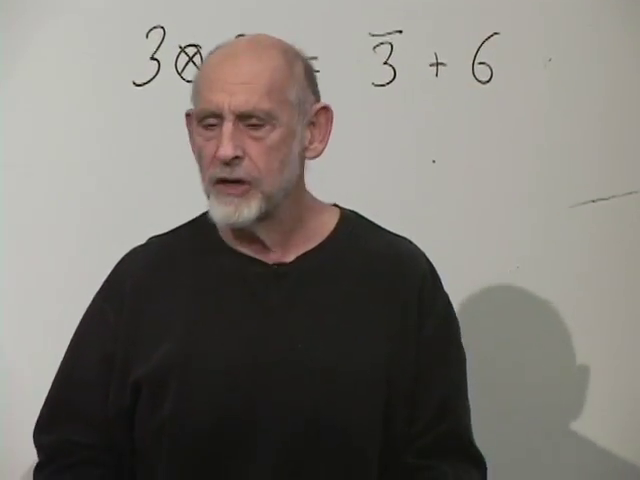
\includegraphics[width=0.68\textwidth]{lecture_04_figure_04.png}
\caption{Произведение двух кварков распадается на антитриплет и секстет.}
\lectureframe{00:39:33}
\end{figure}

Антитриплет можно явно представить, свёртывая два кварковых
индекса с инвариантным тензором эпсилон,
\begin{equation}
(qq)^k_{\bar 3}
=\frac{1}{\sqrt2}\epsilon^{kij}q_iq_j.
\end{equation}
Этот объект имеет 3 компоненты и преобразуется как антикварк. Шесть
симметричных комбинаций образуют секстет. Смысл не в том, что два кварка динамически
превращаются в антикварк; смысл в том, что один сектор их цветовой волновой
функции имеет тот же закон преобразования, что и антикварк.

\subsection{Кварк и антикварк: \texorpdfstring{\(\boldsymbol 3\otimes\bar{\boldsymbol 3}\)}{3 x анти-3}}

Цветовое состояние кварк--антикварк можно рассматривать как \(3\times3\)-матрицу
\(M_i{}^j=q_i\bar q^j\). Всякая такая матрица единственным образом разлагается на следовую и
бесследовую части,
\begin{equation}
M=\frac{\operatorname{tr}M}{3}\boldsymbol 1
+\left(M-\frac{\operatorname{tr}M}{3}\boldsymbol 1\right).
\end{equation}
След — это одна инвариантная компонента, а бесследовая часть имеет 8
компонент. Поэтому
\begin{equation}
\boldsymbol 3\otimes\bar{\boldsymbol 3}
=\boldsymbol 1\oplus\boldsymbol 8.
\label{eq:l4-three-times-threebar}
\end{equation}
С точностью до нормировки синглет имеет вид
\begin{equation}
\ket{1}_{q\bar q}
=\frac{1}{\sqrt3}
(\ket{r\bar r}+\ket{g\bar g}+\ket{b\bar b}).
\end{equation}
Он не может смешаться ни с чем другим, поскольку инвариантен. Остальные 8
линейных комбинаций перемешиваются между собой. Они реализуют присоединённое
представление, то самое представление, в котором преобразуются 8
генераторов.

\subsection{Три кварка}

Добавим третий кварк к разложению из уравнения~\eqref{eq:l4-three-times-three}. Ветвь
антитриплета даёт
\begin{equation}
\bar{\boldsymbol 3}\otimes\boldsymbol 3
=\boldsymbol 1\oplus\boldsymbol 8,
\end{equation}
так что произведение трёх кварков содержит синглет. Полностью имеем,
\begin{equation}
\boldsymbol 3\otimes\boldsymbol 3\otimes\boldsymbol 3
=\boldsymbol 1\oplus\boldsymbol 8\oplus\boldsymbol 8
\oplus\boldsymbol{10}.
\label{eq:l4-three-quark-full}
\end{equation}
Цветовой синглет — это полностью антисимметричная комбинация красный--зелёный--синий,
\begin{equation}
\ket{1}_{qqq}
=\frac{1}{\sqrt6}\epsilon^{ijk}\ket{q_iq_jq_k}.
\label{eq:l4-baryon-singlet}
\end{equation}
Поскольку \(\epsilon^{ijk}\) обращается в нуль всякий раз, когда два индекса совпадают, каждый
ненулевой член содержит один красный, один зелёный и один синий кварк, причём знаки
чередуются при перестановке.

\begin{classroomqa}
\audiencequestion{Разве несинглетные комбинации просто маловероятны, так что их вероятностями можно пренебречь?
\lecturetimestamp{00:46:02}}
\lecturerresponse{Нет. Дело в энергии, а не в малой вероятности. Изолированный несинглет протягивал бы цветовое поле на сколь угодно большие расстояния и в режиме конфайнмента требовал бы неограниченной энергии. Динамика, стоящая за этим утверждением, будет развита ниже.}
\end{classroomqa}

\subsection{Октет глюонов}

Глюонное поле преобразуется как октет в уравнении~\eqref{eq:l4-three-times-threebar}. По отношению к цвету оно несёт
один триплетный индекс и один антитриплетный индекс, причём синглетная следовая часть удалена.
Схематически,
\begin{equation}
q\sim\boldsymbol 3,
\qquad
\bar q\sim\bar{\boldsymbol 3},
\qquad
G\sim\boldsymbol 8.
\end{equation}
Эти символы обозначают законы преобразования; частицы не равны буквально
целым числам 3 и 8.

Девятая цветовая комбинация кварк--антикварк, пропорциональная единичной матрице,
является синглетом и не смешивается с октетом. Поэтому её опущение
математически непротиворечиво: калибровочное поле \(SU(3)\) бесследово и имеет 8
компонент, а не 9, как калибровочное поле \(U(3)\).

\begin{classroomqa}
\audiencequestion{Почему природа не включает дополнительный синглетный глюон?
\lecturetimestamp{00:49:00}}
\lecturerresponse{Непосредственный ответ теории групп таков: синглет образует отдельный инвариантный сектор, поэтому октет замкнут и без него. Более глубокая причина выбора \(SU(3)\), а не \(U(3)\), здесь не выводится; это часть калибровочной структуры, выведенной из феноменологии КХД.}
\end{classroomqa}

\section{Цветовые синглеты как адроны}

Свободные частицы сильного взаимодействия с конечной массой являются цветовыми синглетами.
Это не означает, что кварки или глюоны нереальны; это означает, что они не встречаются как
изолированные асимптотические частицы. Элементарные схемы построения синглетов таковы:
\begin{equation}
qqq,
\qquad
q\bar q,
\qquad
GG\ \text{and higher gluonic products}.
\end{equation}
Они приводят соответственно к барионам, мезонам и глюболам. Произведения нескольких
уже бесцветных объектов, разумеется, снова бесцветны, так что из этих ингредиентов можно построить
и более сложные многоадронные состояния.

\begin{classroomqa}
\audiencequestion{Как называются синглеты из трёх кварков и из кварка--антикварка, и могут ли глюоны тоже образовывать синглеты?
\lecturetimestamp{00:51:38}}
\lecturerresponse{Синглет из трёх кварков — это барион; синглет кварк--антикварк — мезон. Глюоны тоже могут объединяться в цветовые синглеты. Простейшие такие сильно взаимодействующие состояния называются глюболами, и в них могут участвовать более двух глюонов.}
\end{classroomqa}

Три кварка со спином 1/2 всегда объединяются в состояние с суммарным полуцелым спином, хотя орбитальный угловой момент может изменить, какое именно полуцелое значение реализуется. Мезоны кварк--антикварк имеют целый спин. Глюболы, состоящие только из глюонов, также имеют целый спин.

В случае двух глюонов первое утверждение на доске — это лишь подсчёт,
\begin{equation}
8\times8=1+63.
\end{equation}
Всего имеется 64 цветовых состояния; одна комбинация является синглетом, а остальные 63 принадлежат несинглетным секторам.

\begin{figure}[htbp]
\centering
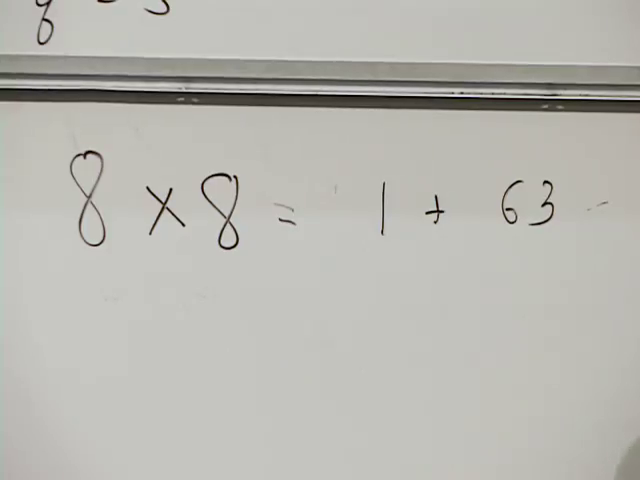
\includegraphics[width=0.68\textwidth]{lecture_04_figure_05.png}
\caption{Подсчёт числа состояний двух глюонов на доске: один синглет среди 64 состояний.}
\lectureframe{00:53:44}
\end{figure}

Полное разложение на неприводимые представления имеет вид
\begin{equation}
\boldsymbol 8\otimes\boldsymbol 8
=\boldsymbol 1\oplus\boldsymbol 8_S\oplus\boldsymbol 8_A
\oplus\boldsymbol{10}\oplus\overline{\boldsymbol{10}}
\oplus\boldsymbol{27}.
\label{eq:l4-eight-times-eight}
\end{equation}
Размерности складываются правильно:
\begin{equation}
1+8+8+10+10+27=64.
\end{equation}
Два октета — разные инвариантные подпространства: одно симметрично, другое антисимметрично при перестановке двух множителей в присоединённом представлении. Синглет — это двухглюонный цветовой канал, из которого можно построить состояние глюбола.
\editorialnote{На доске сначала дано только \(8\times8=1+63\). Более поздний обмен репликами в аудитории добавляет приведённые размерности неприводимых представлений; черты сверху и обозначения симметрии здесь восстановлены в стандартных обозначениях \(SU(3)\).}

\subsection{Почему наблюдаемые электрические заряды целочисленны}

Заряды кварков бывают двух типов,
\begin{equation}
Q_{\mathrm{up\text{-}like}}=+\frac23,
\qquad
Q_{\mathrm{down\text{-}like}}=-\frac13.
\end{equation}
Поэтому суммарный заряд трёх кварков является целым: \(-1,0,+1,\text{ or }+2\),
в зависимости от того, сколько из них относятся к up-типу. Пара кварк и антикварк аналогично имеет
заряд \(0\) или \(\pm1\). Глюоны не несут электрического заряда. Следовательно, базовые цветовые
синглеты, построенные из наблюдаемых кварковых представлений, имеют целочисленный электрический
заряд, хотя их составляющие несут дробный заряд.

\begin{classroomqa}
\audiencequestion{Каков электрический заряд странного кварка?
\lecturetimestamp{00:56:08}}
\lecturerresponse{Он относится к down-типу, поэтому его заряд равен \(-1/3\). Во всех трёх семействах повторяется одна и та же схема зарядов: \((u,d)\), \((c,s)\) и \((t,b)\), с зарядами \(+2/3\) и \(-1/3\) в каждой паре.}
\end{classroomqa}

Цветовая синглетность и целочисленность электрического заряда при таком наборе частиц тесно связаны, но это не тождественные математические утверждения. Целочисленность также опирается на только что записанные конкретные присвоения электрических зарядов в Стандартной модели.

\begin{classroomqa}
\audiencequestion{Является ли цветовой синглет запутанным состоянием, и имеет ли это тот же смысл, что и запутанная пара в эксперименте Белла?
\lecturetimestamp{00:56:58}}
\lecturerresponse{Синглетная цветовая волновая функция, безусловно, является запутанной: это когерентная суперпозиция, а не произведение отдельно определённых цветов. В принципе её составляющие можно разделить, но конфайнмент делает такое разделение всё более энергетически затратным и в конечном счёте порождает новые адроны. Поэтому это не удобная система для манипуляций в стиле эксперимента Белла, хотя само состояние запутано.}
\end{classroomqa}

\section{Что означают уравнения с тензорным произведением}

На этом этапе таблицы умножения заслуживают более конкретного объяснения.
Пусть \(\psi_i\) и \(\phi_j\) — операторы, создающие два объекта со спином 1/2; они могут описывать два вида частиц, например электрон и протон, либо две копии одного и того же вида, если учтена соответствующая статистика.
Каждый индекс принимает два значения. Четыре произведения
\begin{equation}
\psi_\uparrow\phi_\uparrow,
\quad
\psi_\uparrow\phi_\downarrow,
\quad
\psi_\downarrow\phi_\uparrow,
\quad
\psi_\downarrow\phi_\downarrow
\end{equation}
натягивают пространство тензорного произведения.

Если элемент группы действует как \(U\) на каждом сомножителе, то на
произведение он действует как \(U\otimes U\). В компонентах,
\begin{equation}
\psi_i\phi_j
\longmapsto
U_i{}^kU_j{}^\ell\psi_k\phi_\ell.
\label{eq:l4-product-action}
\end{equation}
Это четырёхмерное представление, но оно приводимо. Антисимметричная комбинация
\begin{equation}
\frac{1}{\sqrt2}
(\psi_\uparrow\phi_\downarrow
-\psi_\downarrow\phi_\uparrow)
\end{equation}
переходит в себя, тогда как три симметричные комбинации переходят друг в друга. В базисе, согласованном с этими комбинациями, каждая матрица
представления на произведении имеет блочно-диагональный вид,
\begin{equation}
D_{2\otimes2}(g)
\sim
\begin{pmatrix}
1&0\\
0&D_3(g)
\end{pmatrix}.
\label{eq:l4-spin-block-diagonal}
\end{equation}

\begin{classroomqa}
\audiencequestion{Какая операция представлена уравнением вида \(\boldsymbol 3\otimes\boldsymbol 3=\bar{\boldsymbol 3}\oplus\boldsymbol 6\)?
\lecturetimestamp{00:57:51}}
\lecturerresponse{Левая часть задаёт пространство составных состояний. Группа действует на оба сомножителя и потому перемешивает базисные состояния произведения. Правая часть говорит, что смена базиса разделяет эти состояния на инвариантные наборы: 3 антисимметричные комбинации, преобразующиеся как антитриплет, и 6 симметричных комбинаций, преобразующихся как секстет. Знак плюс означает прямую сумму альтернатив, а не обычное численное сложение.}
\end{classroomqa}

\begin{classroomqa}
\audiencequestion{Откуда мы знаем, что 9 состояний распадаются как \(3+6\) или \(1+8\), а не, скажем, как \(2+7\)?
\lecturetimestamp{01:04:39}}
\lecturerresponse{Одного лишь подсчёта размерностей недостаточно, чтобы определить разбиение. Нужно знать, какими неприводимыми представлениями обладает \(SU(3)\), и построить инвариантные подпространства, например симметризуя индексы, антисимметризуя их или отделяя следовую часть от бесследовой. Полная классификация требует большей теории групп; здесь мы используем только представления, нужные для кварков и глюонов.}
\end{classroomqa}

Инвариантный тензор эпсилон делает построение синглета наглядным. Для
\(SU(2)\),
\begin{equation}
\epsilon_{ij}U^i{}_kU^j{}_\ell
=(\det U)\epsilon_{k\ell}
=\epsilon_{k\ell}.
\end{equation}
Следовательно, \(\epsilon_{ij}\psi^i\phi^j\) инвариантно. Для \(SU(3)\)
трёхиндексная версия даёт
\begin{equation}
\epsilon_{ijk}U^i{}_aU^j{}_bU^k{}_c
=(\det U)\epsilon_{abc}
=\epsilon_{abc},
\end{equation}
что доказывает инвариантность трёхкваркового состояния в
уравнении~\eqref{eq:l4-baryon-singlet}.

\begin{classroomqa}
\audiencequestion{Можно ли явно показать, почему синглет не преобразуется?
\lecturetimestamp{01:07:18}}
\lecturerresponse{Да. Сверните все фундаментальные индексы с полностью антисимметричным тензором эпсилон. При преобразовании произведение матриц умножает эпсилон на \(\det U\). Для специальной унитарной матрицы этот определитель равен единице, так что свёрнутое состояние не изменяется. В \(SU(2)\) это доказывает синглет двух спинов; в \(SU(3)\) — красный--зелёный--синий трёхкварковый синглет.}
\end{classroomqa}

\begin{classroomqa}
\audiencequestion{Каково полное разложение двух глюонных октетов?
\lecturetimestamp{01:09:24}}
\lecturerresponse{Это разложение из уравнения~\eqref{eq:l4-eight-times-eight}: один синглет, два октета, декуплет, антидекуплет и 27-мерное представление. Существует ровно одна цветовая синглетная комбинация двух октетных индексов.}
\end{classroomqa}

\begin{classroomqa}
\audiencequestion{Каково соответствующее полное разложение для трёх кварков?
\lecturetimestamp{01:11:51}}
\lecturerresponse{Физически существенный ответ состоит в том, что оно содержит один синглет. Полное вычисление даёт уравнение~\eqref{eq:l4-three-quark-full}: один синглет, два октета и один декуплет, всего \(1+8+8+10=27\) состояний.\editorialnote{Во время этого обмена репликами лектор не вспоминает полного разложения \(3\otimes3\otimes3\). Стандартное дополнение приведено здесь явно и помечено как редакторское, а не приписано устному ответу.}}
\end{classroomqa}

Та же идея распространяется и на пространство двух глюонов. В наивном базисе тензорного произведения
\(SU(3)\) действует посредством матриц \(64\times64\). В базисе, согласованном с
неприводимыми компонентами, эти матрицы блочно-диагональны,
\begin{equation}
\begin{aligned}
D_{8\otimes8}(g)
&\sim
\operatorname{diag}\bigl(
1,D_{8_S}(g),D_{8_A}(g),
\\
&\hspace{4.8em}
D_{10}(g),D_{\overline{10}}(g),D_{27}(g)
\bigr).
\end{aligned}
\end{equation}
Ни один блок не смешивается с другим, хотя состояния внутри каждого блока смешиваются между
собой.

\begin{classroomqa}
\audiencequestion{Является ли разложение тензорного произведения просто переходом к базису, в котором большая матрица представления становится блочно-диагональной?
\lecturetimestamp{01:12:02}}
\lecturerresponse{Именно так. Для двух спинов четырёхмерная матрица превращается в одномерный синглетный блок и трёхмерный триплетный блок. Для двух глюонов 64-мерная матрица превращается в блоки размерностей \(1,8,8,10,10,\text{ and }27\). Каждый блок замкнут относительно любого группового преобразования.}
\end{classroomqa}

\begin{classroomqa}
\audiencequestion{Есть ли название у одной из таких замкнутых частей внутри полного пространства тензорного произведения?
\lecturetimestamp{01:14:55}}
\lecturerresponse{Это инвариантное подпространство, несущее подпредставление. Если его нельзя разложить дальше, оно несёт неприводимое представление, или ирреп. Полное тензорное произведение есть прямая сумма этих неприводимых компонент.\editorialnote{В источнике искомый термин в аудитории так и не произносится. В ответе приведена стандартная терминология теории представлений.}}
\end{classroomqa}

\begin{classroomqa}
\audiencequestion{Когда несинглетные десятиплеты и другие представления называют несуществующими, означает ли это, что ими следует полностью пренебречь?
\lecturetimestamp{01:15:36}}
\lecturerresponse{Они являются законными цветовыми секторами и важны в промежуточных вычислениях, но не появляются в лаборатории как изолированные частицы конечной энергии. Конфайнмент, а не какой-либо изъян теории представлений, не даёт им стать свободными асимптотическими состояниями.}
\end{classroomqa}

\section{От идеи цвета Намбу к конфайнменту}

Идея цвета возникла раньше окончательной формулировки КХД. Ёитиро Намбу уже
в начале 1960-х годов понял, что скрытое квантовое число, принимающее три значения, могло
решить поразительную проблему: кварки несут дробный электрический заряд, однако свободных
частиц с дробным зарядом не наблюдается. Если физические состояния вынуждены
быть цветовыми синглетами, кварки встречаются в описанных выше комбинациях с
целым зарядом. Оставшийся вопрос — динамический: что вынуждает все свободные
состояния конечной энергии быть синглетами?

Начнём с электромагнитной аналогии. Заряд и противоположный ему заряд притягиваются. Если сближать их, энергия уменьшается; чтобы сблизить одноимённые заряды, нужно совершить работу. Само поле запасает положительную энергию,
\begin{equation}
E_{\mathrm{field}}
=\frac12\int d^3x\,\boldsymbol E^2
\end{equation}
в простых электростатических единицах. При ненулевом суммарном заряде поле простирается далеко за пределы системы, тогда как у тесно связанной нейтральной пары есть лишь короткодействующее дипольное поле. Поэтому нейтрализация убирает энергию поля из внешней области.

Представим, что электромагнитное взаимодействие стало чрезвычайно сильным. Энергетическая цена поля за ненулевой суммарный заряд стала бы настолько большой, что низкоэнергетические объекты в подавляющем большинстве были бы нейтральными, а извлечение заряженной составной части могло бы стать непомерно дорогим. Nambu перенёс эту интуицию на цвет: восемь цветовых зарядов являются источниками восьми глюонных полей, так что большая энергия цветового поля могла бы запретить существование изолированных несинглетов.

Эта интуиция по существу верна, но в QCD есть решающая новая особенность. Фотон не несёт электрического заряда, тогда как глюон несёт цвет. Фотон не является источником классического электромагнитного поля, а уравнения Максвелла линейны: две электромагнитные волны складываются по принципу суперпозиции и проходят друг сквозь друга. Глюон преобразуется по октетному представлению цвета, поэтому глюоны являются источниками других глюонов и взаимодействуют с ними. Даже разные части одного и того же глюонного поля взаимодействуют. Следовательно, неабелево калибровочное поле нелинейно.

\subsection{Трубки потока и линейный потенциал}

На больших расстояниях самодействие глюонов не позволяет цветовому потоку расплываться, как обычное электрическое дипольное поле. Поток сжимается в трубку, соединяющую кварк с антикварком. Напряжённость поля и площадь поперечного сечения длинной трубки приблизительно постоянны, поэтому в ней запасается приблизительно постоянная энергия на единицу длины. Если \(\sigma\) обозначает это натяжение струны, то
\begin{equation}
V(R)\simeq\sigma R+\text{constant}
\qquad (R\ \text{large}).
\label{eq:l4-linear-potential}
\end{equation}

\begin{figure}[htbp]
\centering
\includegraphics[width=0.78\textwidth]{lecture_04_figure_06.png}
\caption{Цветовой поток собран в длинную трубку между кварком и антикварком.}
\lectureframe{01:31:35}
\end{figure}

Такой потенциал сильнее кулоновского, модуль которого убывает как \(1/R\).
Если раздвигать цветовые источники дальше, сила не убывает неограниченно; трубка удлиняется, и энергия продолжает расти. Одинокий цветовой заряд в бесконечном объёме потребовал бы трубку, тянущуюся без конца, и, следовательно, неограниченную энергию. В этом и состоит практический смысл утверждения, что только цветовые синглеты имеют асимптотические состояния с конечной энергией.
\editorialnote{Обозначение натяжения струны и явный вид потенциала на больших расстояниях количественно выражают утверждение источника о том, что однородная трубка потока несёт однородную энергию на единицу длины.}

\subsection{Разрыв струны и джеты}

Предположим, что жёсткое столкновение приходится на один из кварков внутри мезона. Кварк начинает удаляться, но позади него растягивается трубка потока. Он может потерять свою кинетическую энергию, и его втянут обратно. Однако чаще, как только запасённая энергия поля становится достаточно большой, вакуум рождает новую пару кварк--антикварк. Новый антикварк служит концом потока, связанного с уходящим кварком, а новый кварк — концом потока, связанного с исходным антикварком. Один растянутый синглет превращается в два более коротких синглета,
\begin{equation}
(q\bar q)_{\mathrm{stretched}}
\longrightarrow
(q\bar q)+(q\bar q).
\label{eq:l4-string-breaking}
\end{equation}

\begin{figure}[htbp]
\centering
\includegraphics[width=0.78\textwidth]{lecture_04_figure_07.png}
\caption{Рождение пары разрывает одну растянутую трубку потока на две цветосинглетные трубки.}
\lectureframe{01:34:52}
\end{figure}

\begin{classroomqa}
\audiencequestion{Если выбитый кварк имеет достаточно энергии, чтобы продолжать растягивать трубку, что ещё может произойти, кроме того, что его втянут обратно?
\lecturetimestamp{01:33:50}}
\lecturerresponse{Трубка может разорваться за счёт рождения пары кварк--антикварк. Её энергия превращается в массу и кинетическую энергию новой пары. Концы пересоединяются в два синглета, так что процесс порождает дополнительные мезоны, а не изолированный кварк.}
\end{classroomqa}

Если один из этих партонов всё ещё несёт большой импульс, процесс повторяется. Результатом становится каскад цветосинглетных адронов, коллимированный вокруг исходного направления партона: джет. Это превращение энергичных кварков и глюонов в адроны называется адронизацией. Об инициирующем цветном объекте судят по джету; сам по себе он никогда не наблюдается.

\begin{classroomqa}
\audiencequestion{При разрыве струны образуются только мезоны или в джете могут появляться и другие адроны?
\lecturetimestamp{01:35:20}}
\lecturerresponse{Конечно, могут появляться и другие адроны. Единственное цветовое требование состоит в том, чтобы конечные наблюдаемые объекты были синглетами. Мезоны — самый простой вариант для одного разрыва, но могут также рождаться барионы, антибарионы и более сложные синглетные комбинации.}
\end{classroomqa}

Три кварка могут замыкать свои потоки в цветосинглетном узле. Трёхветвенная картина является динамическим аналогом антисимметричного эпсилон-тензора в уравнении~\eqref{eq:l4-baryon-singlet}: из полного бариона не выходит никакого суммарного цветового потока.

\begin{figure}[htbp]
\centering
\includegraphics[width=0.72\textwidth]{lecture_04_figure_08.png}
\caption{Трёхветвевой узел цветового потока для бариона, под схемой разрыва мезонной струны.}
\lectureframe{01:36:12}
\end{figure}

\section{Калибровочные поля, сохраняющиеся заряды и стандартная модель}

На данном уровне калибровочную теорию можно понимать как теорию, в которой сохраняющийся заряд является источником фотоноподобного поля. Электрический заряд является источником электромагнитного поля; восемь цветовых зарядов являются источниками восьми глюонных полей. Более глубокая формулировка делает симметрию локальной и вводит связность, которая сравнивает внутренние состояния в соседних точках пространства-времени, но для развиваемой здесь картины конфайнмента эта конструкция не нужна.
\editorialnote{Формулировка через локальную симметрию — это тот стандартный, более глубокий смысл калибровочной теории, на который источник ссылается, но который сознательно откладывает.}

Симметрия, сохраняющийся заряд и поток тесно связаны. Если силовые линии поля могут оканчиваться только на зарядах, то источник не может просто исчезнуть, оставив свой поток оборванным. Не может и всё его удалённое поле исчезнуть мгновенно, потому что изменения поля распространяются причинно. В локальной форме та же физика выражается уравнением непрерывности,
\begin{equation}
\frac{\partial\rho}{\partial t}
+\boldsymbol\nabla\cdot\boldsymbol j=0,
\end{equation}
которое говорит, что заряд может покинуть область, только перетекая через её границу. Аргумент через силовые линии — это геометрическая картина этого локального закона сохранения.

Теперь мы можем поместить результат в рамки стандартной модели. Цвет даёт восемь генераторов \(SU(3)\) и соответствующие им восемь глюонных полей. Абелев сектор даёт один генератор и одно калибровочное поле. Ещё три генератора принадлежат дополнительной группе \(SU(2)\), а не обычному пространственному угловому моменту. До нарушения симметрии калибровочная структура имеет вид
\begin{equation}
SU(3)_c\times SU(2)_L\times U(1)_Y,
\end{equation}
с \(8+3+1=12\) генераторами. Следующая задача — понять электрослабую группу \(SU(2)\), затем поле Хиггса и то, как возникают наблюдаемые фотон, \(W^\pm\) и \(Z\).
\editorialnote{Источник считает фотон вместе с восемью глюонами и описывает оставшийся множитель как \(SU(2)\times U(1)\). В ненарушенной стандартной модели абелевым множителем является гиперзаряд \(U(1)_Y\); фотон появляется только после электрослабого смешивания.}

Теперь центральная цепочка завершена. Абстрактные группы действуют через представления; бесконечно малые генераторы являются сохраняющимися зарядами; кварки, антикварки и глюоны реализуются в \(\boldsymbol 3\), \(\bar{\boldsymbol 3}\) и \(\boldsymbol 8\); тензорные произведения выделяют адроны-синглеты; а нелинейное глюонное поле превращает отбор синглетов в физическое явление конфайнмента.
\chapter{Калибровочные поля, масштабы взаимодействия и заряженные слабые токи}

Квантовая электродинамика и квантовая хромодинамика в лаборатории выглядят очень по-разному, однако обе являются калибровочными теориями. Более того, почти каждое взаимодействие в стандартной модели устроено именно так. Слово \emph{gauge} имеет более глубокий смысл, связанный с локальной симметрией, но этот аппарат мы пока можем отложить. Сейчас нам нужно минимальное физическое описание: калибровочная теория содержит поля, подобные максвелловским, сохраняющиеся источники, преобразования симметрии, калибровочные бозоны и правила испускания и поглощения этих бозонов.

\section{Теория Максвелла как прототип}

\subsection{Поля и потенциалы}

Электромагнитное поле имеет шесть компонент: три компоненты электрического поля и три компоненты магнитного поля. Та же информация, с некоторой избыточностью, может быть закодирована в четырёхвекторном потенциале
\begin{equation}
A_\mu=(A_0,\boldsymbol A),
\end{equation}
где \(A_0\) — электростатический потенциал, а \(\boldsymbol A\) — пространственный векторный потенциал. В электростатическом пределе электрическое поле получается из пространственного градиента,
\begin{equation}
\boldsymbol E=-\boldsymbol\nabla A_0,
\qquad
\boldsymbol F=q\boldsymbol E,
\end{equation}
тогда как магнитное поле равно
\begin{equation}
\boldsymbol B=\boldsymbol\nabla\times\boldsymbol A.
\end{equation}
Знак в первом уравнении зависит от принятого стандартного определения потенциала; обсуждение у доски в основном касается того факта, что поля являются производными потенциалов.
\editorialnote{Для зависящих от времени полей полное соотношение имеет вид
\(\boldsymbol E=-\boldsymbol\nabla A_0-\partial_t\boldsymbol A\). Здесь в лекции намеренно рассматривается более простой электростатический уровень.}

\begin{figure}[htbp]
\centering
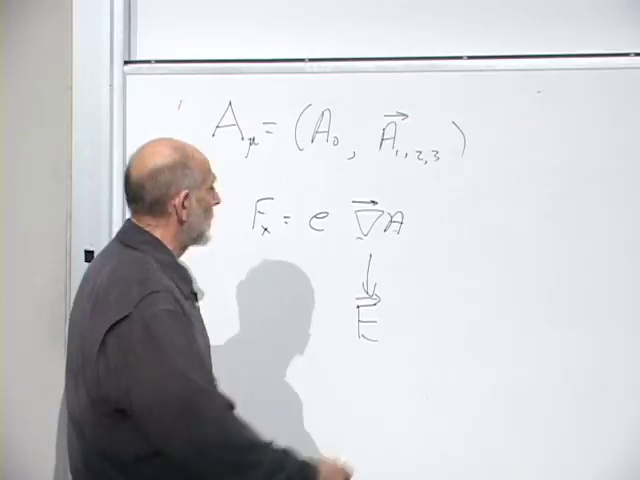
\includegraphics[width=0.62\textwidth]{lecture_05_figure_02.png}
\caption{Электромагнитный четырёхпотенциал и его связь с полем через производные.}
\lectureframe{00:03:33}
\end{figure}

Таким образом, электродинамика допускает два эквивалентных описания: одно через \(\boldsymbol E\) и \(\boldsymbol B\), а другое через \(A_\mu\). Во втором явно выписаны только четыре компоненты, потому что одни и те же физические поля могут описываться разными потенциалами. Эта избыточность — первый намёк на смысл слова калибровка, хотя формально мы этим пока пользоваться не будем.

\subsection{Волны и поляризация}

Уравнения Максвелла допускают волны. Рассмотрим плоскую волну, распространяющуюся вдоль единичного вектора \(\hat{\boldsymbol k}\). В каждой точке электрическое и магнитное поля поперечны:
\begin{equation}
\boldsymbol E\cdot\hat{\boldsymbol k}=0,
\qquad
\boldsymbol B\cdot\hat{\boldsymbol k}=0,
\qquad
\boldsymbol E\cdot\boldsymbol B=0.
\end{equation}
В единицах, где \(c=1\), их модули равны,
\begin{equation}
|\boldsymbol E|=|\boldsymbol B|.
\end{equation}
Для линейно поляризованной волны направление \(\boldsymbol E\) задаёт поляризацию. Вся конфигурация распространяется со скоростью света.

Квантование меняет язык описания, но не структуру поляризации. Квант электромагнитной волны — это фотон. Изображать фотон точкой неизбежно вводит в заблуждение, но полезно вообразить, что эта точка несёт маленькую поперечную стрелку, фиксирующую его поляризацию. Четвертьволновая пластинка или другой оптический элемент может поворачивать её. Статическое кулоновское поле аналогичным образом тоже можно, хотя лишь грубо, представлять как возникающее из многократного испускания и поглощения фотонов.

\subsection{Источники, поток и сохранение}

Электромагнитные волны могут распространяться в пустом пространстве, но у поля есть и источники: электрические заряды и токи. Положительный точечный заряд создаёт направленное наружу радиальное электрическое поле, пропорциональное \(1/r^2\). Число силовых линий, проходящих через любую сферу вокруг заряда, не зависит от радиуса этой сферы. Математически,
\begin{equation}
\oint_{S^2}\boldsymbol E\cdot d\boldsymbol S
=\frac{Q_{\mathrm{enc}}}{\epsilon_0},
\label{eq:l5-gauss}
\end{equation}
в единицах СИ.

Это больше, чем просто удобный способ вычислять поле. Линии электрического поля могут оканчиваться только на заряде. Если бы один изолированный заряд просто исчез, его поле либо должно было бы исчезнуть сразу повсюду, нарушая причинность, либо наружу должен был бы распространяться фронт исчезнувшего поля, причём силовые линии оканчивались бы в пустом пространстве. Ни то ни другое недопустимо. Поэтому геометрия потока делает сохранение заряда естественным: заряд может перемещаться, противоположные заряды могут аннигилировать, но суммарный заряд не может локально исчезнуть без компенсирующего тока.

Соответствующее локальное утверждение — это уравнение непрерывности
\begin{equation}
\partial_t\rho+\boldsymbol\nabla\cdot\boldsymbol J=0.
\label{eq:l5-continuity}
\end{equation}
\editorialnote{Уравнение~\eqref{eq:l5-continuity} — это стандартная локальная математическая форма причинного аргумента о потоке, который в лекции излагался словами.}

\subsection{Рабочее определение калибровочной теории}

Теперь мы можем сформулировать рабочую схему. Калибровочная теория имеет:
\begin{itemize}
\item поля, подобные электрическому и магнитному;
\item волны, которые, если взаимодействия достаточно слабы, напоминают световые волны;
\item источники, аналогичные электрическому заряду;
\item закон Гаусса, связывающий поток с этими источниками;
\item закон сохранения и связанную с ним симметрию;
\item кванты поля, называемые калибровочными бозонами; и
\item константу связи, управляющую испусканием и поглощением.
\end{itemize}
Источник не обязан быть электрическим зарядом. В качестве заведомо нефизического примера представим, что барионное число сделано калибровочным. И протоны, и нейтроны имеют барионное число \(+1\), так что они отталкивались бы посредством новой кулоноподобной силы; протон и антипротон притягивались бы. Такую теорию можно вообразить математически, но в природе не наблюдается дальнодействующего калибровочного поля, связанного с барионным числом. Само по себе сохранение не гарантирует калибровочную силу.

У электрического заряда действительно есть соответствующая симметрия. Для заряженного поля вещества,
\begin{equation}
\psi(x)\longmapsto e^{i\theta}\psi(x).
\label{eq:l5-u1}
\end{equation}
Фазовая симметрия и сохранение заряда — две стороны одной и той же структуры. Позже мы сможем сделать \(\theta\) зависящей от пространства-времени и увидеть, почему требуется потенциал \(A_\mu\). Здесь глобального преобразования достаточно, чтобы выделить сохраняющийся заряд.

\section{Квантовая хромодинамика как неабелевский пример}

\subsection{Триплеты, антитриплеты и матрица глюонного поля}

В квантовой хромодинамике кварковое поле несёт цветовой индекс \(i\in\{r,g,b\}\) и преобразуется по фундаментальному представлению группы \(SU(3)\):
\begin{equation}
q'_i=U_{ij}q_j,
\qquad
U^\dagger U=\boldsymbol 1,
\qquad
\det U=1.
\label{eq:l5-q-transform}
\end{equation}
Это поворот в трёхмерном комплексном цветовом пространстве, а не поворот обычного координатного пространства. Трёхкомпонентное представление также называют определяющим представлением.

Поля античастиц представляются комплексно-сопряжёнными переменными. Комплексное сопряжение уравнения~\eqref{eq:l5-q-transform} даёт
\begin{equation}
q_i^{\prime *}=U_{ij}^*q_j^*.
\label{eq:l5-antiquark-transform}
\end{equation}
Таким образом, кварки преобразуются как \(\boldsymbol 3\), тогда как антикварки преобразуются как \(\bar{\boldsymbol 3}\).

\begin{figure}[htbp]
\centering
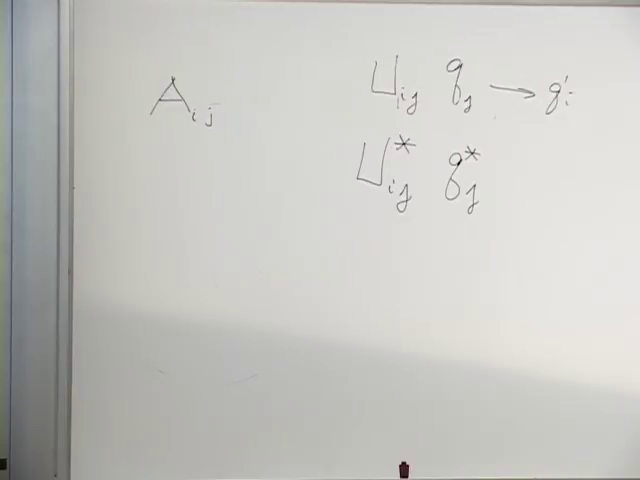
\includegraphics[width=0.62\textwidth]{lecture_05_figure_03.png}
\caption{Фундаментальное преобразование и его комплексно-сопряжённое антитриплетное преобразование.}
\lectureframe{00:18:47}
\end{figure}

\begin{classroomqa}
\audiencequestion{Сколько матриц \(U\) существует -- семь, восемь или девять?
\lecturetimestamp{00:19:37}}
\lecturerresponse{Элементов группы \(U\) бесконечно много. Подсчитываемое конечное число — это число независимых генераторов, и для \(SU(3)\) оно равно восьми. У общей матрицы \(3\times3\) девять позиций, но условие специальной унитарности оставляет восемь непрерывных направлений.}
\end{classroomqa}

Глюонное поле можно записать как матрицу \(A_{ij}\) со нулевым следом. Один индекс преобразуется как у кварка, а другой — как у антикварка, поэтому его цветовая структура имеет вид
\begin{equation}
\boldsymbol 3\otimes\bar{\boldsymbol 3}
=\boldsymbol 1\oplus\boldsymbol 8.
\end{equation}
В КХД сохраняется бесследовый октет,
\begin{equation}
A_{ii}=\operatorname{tr}A=0,
\end{equation}
а синглет отбрасывается. Поэтому в КХД восемь глюонов, а не девять. Более общо, группа \(SU(N)\) имеет
\begin{equation}
N^2-1
\end{equation}
генераторов и столько же полей калибровочных бозонов.

Фотон нейтрален относительно электрического \(U(1)\): поворот фазы электрона не превращает фотон в другой фотон. С глюонами иначе. Глюон несёт цвет и антицвет, поэтому он преобразуется по присоединённому представлению. Например, комбинация красный--антисиний не является цветовым синглетом, хотя в ней есть один цвет и один антицвет.

\subsection{Поток индексов и самовзаимодействие}

Правило взаимодействия можно прочитать, прослеживая индексы. Схематически кварк цвета \(i\) может стать кварком цвета \(j\), испустив глюон, несущий соответствующий поток цвета:
\begin{equation}
q_i\longrightarrow q_j+A_{ij}.
\label{eq:l5-quark-gluon-vertex}
\end{equation}
Точное расположение \(i\) и \(j\) зависит от соглашения о направлении стрелок; инвариантное содержание состоит в том, что каждый индекс, входящий в вершину, должен продолжиться по другой линии. Ни один цветовой индекс не теряется.

Это правило действует в любой калибровочной теории \(SU(N)\). Фундаментальная материя имеет один индекс, антифундаментальная материя имеет один сопряжённый индекс, а калибровочный бозон имеет по одному индексу каждого типа. Физические названия могут меняться, но индексная структура остаётся.

Поскольку глюон сам несёт цвет, он может испустить другой глюон. Глюон \(A_{ij}\) может расщепиться через промежуточный индекс \(k\); схематически,
\begin{equation}
A_{ij}\longrightarrow A_{ik}+A_{kj}.
\label{eq:l5-three-gluon-index}
\end{equation}
Это не полная вершина Янга--Миллса, но она показывает поток цвета. В обычной электродинамике для фотонов ничего аналогичного не происходит. Поэтому глюоны оказывают силовое воздействие друг на друга, и динамика неабелевых полей гораздо сложнее, чем линейная теория Максвелла.

Одно качественное следствие — конфайнмент. Линии потока цветового поля не могут обрываться, и их самодействие стягивает их в трубку, соединяющую кварк с антикварком. Эта трубка несет приблизительно постоянную энергию на единицу длины:
\begin{equation}
V(R)\simeq \sigma R.
\end{equation}
Поэтому, если раздвигать ее концы дальше, запасается все больше энергии, а не высвобождается изолированный цвет. Это и есть картина тягучего клея: само поле не позволяет цветным составляющим вырваться в виде свободных частиц.

\section{Константы связи и смысл слов сильный и слабый}

\subsection{Заряд как амплитуда испускания}

Калибровочной теории все равно нужна константа связи. В КЭД заряд электрона \(e\) — это коэффициент, связанный с вершиной электрон--фотон. Это амплитуда, а вероятности — квадраты амплитуд. Операционально можно представить, что быстрый электрон резко тормозится в электронно-лучевой трубке. Вероятность излучить фотон пропорциональна \(e^2\), причем стандартные множители поглощены в постоянную тонкой структуры,
\begin{equation}
\alpha=\frac{e^2}{4\pi\hbar c}
\simeq \frac{1}{137}.
\label{eq:l5-alpha}
\end{equation}
В естественных единицах \(\hbar=c=1\) константа связи безразмерна. Масштаб порядка одного процента для элементарного акта испускания делает электромагнетизм слабым в пертурбативном смысле: большинство остановленных электронов не испускают целый веер жестких фотонов.

\subsection{Естественные единицы связывают энергию, время и расстояние}

Положим
\begin{equation}
c=1,
\qquad
\hbar=1.
\end{equation}
Тогда время и расстояние имеют одни и те же единицы, а энергия — обратные единицы:
\begin{equation}
E=\hbar\omega\longrightarrow E=\omega\sim\frac1t,
\qquad
x\sim t\sim\frac1E.
\end{equation}
Большие энергии зондируют малые расстояния и короткие времена.

Для ориентировки,
\begin{equation}
1\ {\rm eV}^{-1}
=\frac{\hbar c}{1\ {\rm eV}}
\simeq 1.97\times10^{-7}\ {\rm m}.
\end{equation}
Поэтому атомный масштаб длины порядка \(10^{-10}\ {\rm m}\) приблизительно соответствует обратному килоэлектронвольту. Это пересчеты по порядку величины, а не точная спектроскопия.

\subsection{Иерархия внутри атома}

Для типичного атома возьмем
\begin{equation}
R_{\rm atom}\sim10^{-10}\ {\rm m}.
\end{equation}
Свет проходит это расстояние за
\begin{equation}
t_{\rm transit}^{\rm atom}\sim10^{-18}\ {\rm s}.
\end{equation}
Однако в легком атоме электрон движется лишь с малой долей скорости света. В боровской картине \(v/c\sim\alpha\), поэтому типичное орбитальное время больше:
\begin{equation}
t_{\rm orbit}^{\rm atom}\sim10^{-16}\ {\rm s}.
\end{equation}

Возбужденному атому требуется еще больше времени, чтобы излучить:
\begin{equation}
t_{\rm decay}^{\rm atom}\sim10^{-9}\ {\rm s}
\end{equation}
как грубая оценка на уровне лекции. В физической картине есть два подавляющих фактора. Электромагнитная сила создает лишь умеренное ускорение, а у ускоренного электрона есть еще одна малая вероятность испускания, определяемая \(\alpha\). Поэтому малая постоянная тонкой структуры создает иерархию между временами пролета, орбитального движения и радиационного распада.

\subsection{Отсутствие иерархии в адроне}

Адрон — это атомоподобная связанная система из кварков и глюонов, но ее масштаб гораздо меньше:
\begin{equation}
R_{\rm hadron}\sim10^{-15}\ {\rm m},
\qquad
t_{\rm transit}^{\rm hadron}\sim10^{-23}\ {\rm s}.
\end{equation}
Кварки пересекают адрон практически за то же время, и возбужденные адроны, распадающиеся сильным образом, тоже живут примерно
\begin{equation}
t_{\rm orbit}^{\rm hadron}
\sim t_{\rm decay}^{\rm hadron}
\sim10^{-23}\ {\rm s}.
\end{equation}
Адрон после удара может заколебаться и испустить пион почти настолько быстро, насколько это допускает причинность. Здесь нет разделения на семь или девять порядков величины, как внутри атома.

\begin{classroomqa}
\audiencequestion{Следует ли из специальной теории относительности, что адрон не может распадаться существенно быстрее, чем за время прохождения света через него?
\lecturetimestamp{00:47:15}}
\lecturerresponse{Так вполне корректно формулировать эту оценку по порядку величины. Сильные распады происходят примерно так быстро, как допускает размер системы; нет ни малой константы связи, ни другого большого подавления, которое их замедляло бы.}
\end{classroomqa}

Соответствующая сильная константа связи поэтому намного больше, чем \(\alpha\). На иллюстративном адронном масштабе в лекции приводится
\begin{equation}
\alpha_{\rm QCD}\sim0.2,
\end{equation}
что гораздо ближе к единице, чем \(1/137\). Таково динамическое происхождение более старого названия \emph{сильные взаимодействия}.
\editorialnote{Константа связи КХД зависит от энергии, поэтому \(\alpha_s\) не является одним фиксированным числом. Приведенное значение — иллюстративное зависящее от масштаба значение, как и подразумевается в лекции.}

\begin{classroomqa}
\audiencequestion{Называют ли сильный аналог просто константой сильного взаимодействия?
\lecturetimestamp{00:48:17}}
\lecturerresponse{По принятому соглашению ее называют \(\alpha_{\rm QCD}\) или, чаще, \(\alpha_s\). Электромагнитную обычно обозначают просто \(\alpha\), хотя \(\alpha_{\rm QED}\) можно использовать, когда обе появляются в одном и том же обсуждении.}
\end{classroomqa}

\begin{classroomqa}
\audiencequestion{Будет ли статья различать голую электромагнитную константу связи и измеренное, экранированное значение?
\lecturetimestamp{00:48:38}}
\lecturerresponse{Да. Говорят о голой константе связи и о перенормированной константе связи. Поляризация вакуума делает эффективную константу связи зависящей от масштаба, на котором она измеряется.}
\end{classroomqa}

\section{Загадка слабого распада}

Слабые взаимодействия получили свое название из-за связанных с ними очень больших времен распада. Обычно они медленнее сильных распадов и могут быть медленнее даже атомного излучения. Старейший пример — ядерный бета-распад.

\subsection{Нейтронный бета-распад}

Свободный нейтрон распадается по схеме
\begin{equation}
n\longrightarrow p+e^-+\bar\nu_e.
\label{eq:l5-neutron-decay-intro}
\end{equation}
На лекции используется время жизни порядка двенадцати минут, абсурдно большое по сравнению с \(10^{-23}\ {\rm s}\). Современные точные значения для этого рассуждения несущественны.

Часть этой медленности кинематическая. Грубо говоря,
\begin{equation}
\begin{aligned}
m_n&\simeq940\ {\rm MeV},
&
m_p&\simeq939\ {\rm MeV},
\\
m_e&\simeq0.5\ {\rm MeV}.
\end{aligned}
\end{equation}
Лишь ничтожная доля энергии покоя нейтрона доступна как кинетическая энергия. Если бы нейтрон был легче суммы конечных масс покоя, распад был бы невозможен. Если бы он находился лишь бесконечно мало выше порога, доступное фазовое пространство было бы крошечным, и распад был бы медленным. Но одно лишь фазовое пространство не может объяснить время жизни, измеряемое минутами.

\subsection{Заряженный пион устраняет оправдание порогом}

Рассмотрим также
\begin{equation}
\pi^-\longrightarrow e^-+\bar\nu_e
\end{equation}
и его зарядово-сопряженный процесс. У пиона имеется большой избыток энергии для электронного канала, однако его слабое время жизни все равно имеет порядок наносекунд, а не адронный порядок \(10^{-23}\) секунды. Сходный канал с мюоном вскоре станет важным. Следовательно, загадка присуща самому слабому взаимодействию, а не является просто случайностью почти вырожденных масс в нейтронном случае.

\editorialnote{Время жизни заряженного пиона составляет около \(26\ {\rm ns}\), а доминирующим каналом является \(\pi^-\to\mu^-\bar\nu_\mu\). Электронный канал подавлен по спиральности. На лекции сначала используется электронный канал, поскольку в нем проще всего вести учет частиц, а затем рассмотрение возвращается к доминирующему мюонному каналу.}

Термин бета-распад исторически возник из того, что испускаемые электроны называли бета-лучами. Примеры с пионом и нейтроном включают одно и то же взаимодействие заряженного тока, хотя их кинематика резко различается.

\section{Таблица кварков и лептонов}

\subsection{Цвет действует по вертикали}

Расположим шесть ароматов кварков в трех парных столбцах,
\begin{equation}
(u,d),\qquad(c,s),\qquad(t,b),
\end{equation}
и поместим красную, зеленую и синюю копию каждого кварка в отдельные строки. Цвет \(SU(3)\) действует по вертикали: он вращает друг в друга красную, зеленую и синюю версии u-кварка и одновременно выполняет то же цветовое вращение для d-, c-, s-, t- и b-кварков. Он не превращает u-кварк в d-кварк.

\subsection{Слабый изоспин действует по горизонтали}

Слабая симметрия действует в другом направлении. Она смешивает каждую соседнюю пару
\begin{equation}
Q_1=\begin{pmatrix}u\\d\end{pmatrix},
\qquad
Q_2=\begin{pmatrix}c\\s\end{pmatrix},
\qquad
Q_3=\begin{pmatrix}t\\b\end{pmatrix}.
\label{eq:l5-quark-doublets}
\end{equation}
У кварков верхнего типа заряд \(+2/3\), а у кварков нижнего типа заряд \(-1/3\), так что при переходе через каждую пару заряд меняется на единицу.
\editorialnote{В источнике на мгновение говорится, что d-кварк имеет заряд \(-2/3\). Вычитание в этом месте и все последующие процессы требуют стандартного значения \(-1/3\), которое и используется здесь.}

Поскольку симметрия действует на дублеты, естественной группой является \(SU(2)\). Она действует на каждую цветовую копию каждого кваркового дублета, не изменяя цвет.

Есть и четвертая строка частиц, не несущих цвет и потому не взаимодействующих с глюонами: лептоны. Они образуют еще три дублета,
\begin{equation}
L_e=\begin{pmatrix}\nu_e\\e^-\end{pmatrix},
\qquad
L_\mu=\begin{pmatrix}\nu_\mu\\\mu^-\end{pmatrix},
\qquad
L_\tau=\begin{pmatrix}\nu_\tau\\\tau^-\end{pmatrix}.
\label{eq:l5-lepton-doublets}
\end{equation}
Нейтрино электрически нейтральны; электрон, мюон и тау имеют заряд \(-1\). И здесь оба члена дублета различаются на одну единицу электрического заряда. Электрон, мюон и тау имеют одни и те же калибровочные квантовые числа, но разные массы, подобно тому как три поколения кварков верхнего или нижнего типа повторяют ту же схему зарядов.

\begin{figure}[htbp]
\centering
\includegraphics[width=0.82\textwidth]{lecture_05_figure_05.png}
\caption{Таблица на доске: цвет действует между красной, синей и зеленой строками, тогда как слабое \(SU(2)\) связывает попарно объединенные столбцы ароматов и лептонную строку.}
\lectureframe{01:03:35}
\end{figure}

Называть лептоны четвертым цветом — пока лишь аналогия. Они заполняют четвертую строку в таблице слабых дублетов, но обычная КХД \(SU(3)\) не преобразует кварки в лептоны.

\section{Построение заряженных слабых бозонов}

\subsection{Квантовые числа заряженных бозонов}

Калибровочные бозоны несут свойства преобразования, необходимые для перехода от одного члена дублета к другому. Начнём с лептонной пары
\(e^-\bar\nu_e\). Она имеет электрический заряд \(-1\), поэтому соответствующий заряженный калибровочный бозон называется \(W^-\):
\begin{equation}
W^-\sim e^-\bar\nu_e.
\end{equation}
Те же квантовые числа возникают у d-кварка и анти-u-кварка:
\begin{equation}
W^-\sim d\bar u.
\end{equation}
Символ \(\sim\) означает: имеет те же существенные калибровочные квантовые числа, что и.
Это не означает, что \(W\) буквально является связанным состоянием этих частиц.
Для античастицы получаются сопряжённые комбинации,
\begin{equation}
W^+\sim e^+\nu_e\sim\bar d u.
\end{equation}

Вершины заряженного слабого взаимодействия включают
\begin{align}
e^-&\longrightarrow\nu_e+W^-,
&
\mu^-&\longrightarrow\nu_\mu+W^-,
\label{eq:l5-lepton-w}\\
d&\longrightarrow u+W^-,
&
s&\longrightarrow c+W^-,
\label{eq:l5-quark-w}
\end{align}
с аналогичными переходами для третьего поколения, когда они кинематически разрешены. Калибровочный бозон динамически осуществляет то же горизонтальное смешивание, которое симметрия осуществляет в дублете.

\begin{classroomqa}
\audiencequestion{Сохранение заряда определяет, что испускаемый бозон должен иметь заряд
\(-1\), но почему переходы электрона, d-кварка и s-кварка
все должны включать одну и ту же частицу?
\lecturetimestamp{01:12:56}}
\lecturerresponse{Это эмпирический факт, закодированный общей слабой
симметрией. Природа могла бы непротиворечиво приписать отдельный бозон типа \(W\)
каждому семейству или кваркам и лептонам по отдельности. Вместо этого одно
\(SU(2)\) действует одновременно на все дублеты, и одни и те же заряженные калибровочные
бозоны опосредуют все эти переходы.}
\end{classroomqa}

\subsection{Чтение вершины и её обращение}

Одна вершина представляет целое семейство процессов. Если входящую линию
сделать исходящей, частица превращается в свою античастицу, а обращение линии
\(W^-\) даёт \(W^+\). Поэтому вершину можно читать как испускание,
поглощение, распад, аннигиляцию или обратную реакцию, если последовательно
соблюдать заряд, импульс и все существенные квантовые числа.

\begin{classroomqa}
\audiencequestion{Можно ли перевернуть стрелки и линии в этих слабых вершинах?
\lecturetimestamp{01:14:51}}
\lecturerresponse{Да. Линию можно перенести из конечного состояния в
начальное или наоборот, но тогда частица становится своей античастицей.
Поэтому одна и та же локальная вершина описывает много реакций с различной
ориентацией.}
\end{classroomqa}

\begin{classroomqa}
\audiencequestion{Означает ли запись \(W^-\) с линиями странного и очарованного
кварков, что этот бозон буквально является связанным состоянием странного кварка и
антиочарованного кварка?
\lecturetimestamp{01:15:43}}
\lecturerresponse{Нет. Учёт линий лишь говорит, что \(W^-\) несёт
изменение квантовых чисел между этими столбцами. Если читать диаграмму как
распад, достаточно энергичный \(W^-\) может породить странный кварк и
антиочарованный кварк; он не состоит из них.}
\end{classroomqa}

\begin{classroomqa}
\audiencequestion{Могут ли электрон и антинейтрино образовать \(W\), который затем
породит кварковую пару?
\lecturetimestamp{01:17:22}}
\lecturerresponse{Именно. Если доступна достаточная энергия в системе центра масс,
начальные лептоны могут образовать промежуточное состояние заряженного тока, и это состояние
может реализоваться в разрешённом кварковом канале. Эти две вершины — те же самые,
что используются в распаде, только прочитанные в другой ориентации.}
\end{classroomqa}

\subsection{Недостающий третий бозон}

Группа \(SU(2)\) имеет три генератора, а значит, три калибровочных поля. Пока что мы
явно показали только \(W^+\) и \(W^-\). Третье, электрически нейтральное поле
должно быть связано с диагональными комбинациями, такими как квантовые числа электрона--позитрона и
нейтрино--антинейтрино. Его намеренно оставляют скрытым на заднем
плане. Его связь с физическим бозоном \(Z\) и фотоном требует
электрослабого смешивания, к которому мы перейдём позже.

\begin{classroomqa}
\audiencequestion{Начали ли подозревать существование слабого и сильного взаимодействий в
разные исторические периоды?
\lecturetimestamp{01:24:11}}
\lecturerresponse{Их экспериментальные корни проявились вместе в ранних
исследованиях радиоактивности. Альфа-распад выявил ядерную физику и физику
сильного взаимодействия, бета-распад выявил слабое взаимодействие, а при
гамма-распаде испускались электромагнитные фотоны. В эпоху Беккереля уже
содержались все три указания, задолго до появления их современных полевых теорий.}
\end{classroomqa}

\section{Разобранные распады по заряженному току}

\subsection{Распад пиона}

Отрицательно заряженный пион имеет валентный кварковый состав
\begin{equation}
\pi^-=d\bar u.
\end{equation}
Эти квантовые числа могут аннигилировать в \(W^-\), который затем может породить
заряженный лептон и соответствующее антинейтрино:
\begin{align}
\pi^-&\longrightarrow W^{-*}
\longrightarrow e^-+\bar\nu_e,
\label{eq:l5-pion-electron}\\
\pi^-&\longrightarrow W^{-*}
\longrightarrow \mu^-+\bar\nu_\mu.
\label{eq:l5-pion-muon}
\end{align}
Звёздочка напоминает нам, что промежуточный \(W\) виртуален. Второй канал
является доминирующим.

\begin{figure}[htbp]
\centering
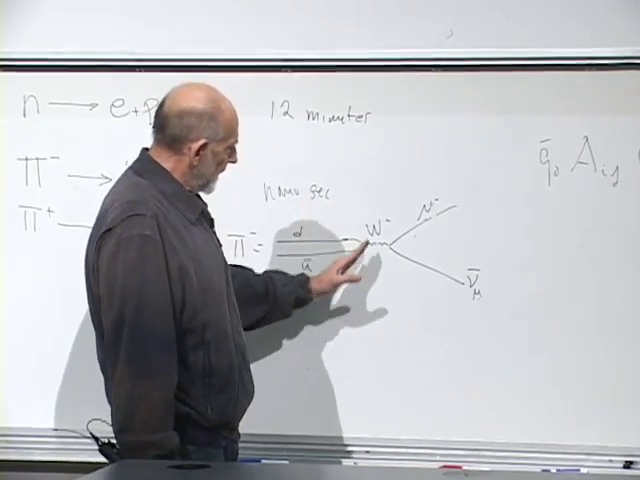
\includegraphics[width=0.72\textwidth]{lecture_05_figure_04.png}
\caption{Пион \(d\bar u\) аннигилирует в виртуальный \(W^-\), после чего
рождаются заряженный лептон и соответствующее ему антинейтрино.}
\lectureframe{01:19:38}
\end{figure}

\begin{classroomqa}
\audiencequestion{Действительно ли это диаграмма Фейнмана, хотя направление
времени нарисовано горизонтально, а не вертикально?
\lecturetimestamp{01:20:21}}
\lecturerresponse{Да. Ориентация времени на странице — дело соглашения.
Как только одно направление объявлено временем и все стрелки интерпретируются
последовательно, рисунок несёт ту же информацию о взаимодействии.}
\end{classroomqa}

\begin{classroomqa}
\audiencequestion{Можно ли читать эту диаграмму скорее как обратимую химическую
реакцию, а не как необратимый односторонний распад?
\lecturetimestamp{01:21:35}}
\lecturerresponse{Обратный процесс разрешён. Пион, возникший в пустом
пространстве, распадается, потому что вылетающие частицы разлетаются и обычно
не рекомбинируют. Но если мюон и антинейтрино направить навстречу друг другу с подходящими
энергией и импульсом, существует ненулевая амплитуда образования пиона через
обратное взаимодействие.}
\end{classroomqa}

\subsection{Энергия и виртуальное промежуточное состояние}

Для покоящегося пиона,
\begin{equation}
m_\pi\simeq140\ {\rm MeV},
\qquad
m_\mu\simeq106\ {\rm MeV},
\qquad
m_\nu\approx0
\end{equation}
с точностью, существенной здесь. Оставшаяся энергия переходит в кинетическую энергию
вылетающих частиц. Сохранение импульса требует
\begin{equation}
\boldsymbol p_\mu+\boldsymbol p_{\bar\nu}=0,
\end{equation}
так что в системе покоя пиона две частицы разлетаются в противоположных направлениях.

\begin{classroomqa}
\audiencequestion{Как может сохраняться энергия, если промежуточный \(W\)
намного тяжелее пиона?
\lecturetimestamp{01:25:08}}
\lecturerresponse{Только начальные и конечные частицы обязаны быть на массовой
оболочке. Четырёхимпульс сохраняется в каждой вершине, но внутренняя виртуальная
линия не обязана удовлетворять \(E^2=\boldsymbol p^2+m_W^2\). Чем больше её отклонение
от массовой оболочки, тем сильнее её пропагатор подавляет процесс.\editorialnote{В лекции используется традиционный язык соотношения неопределённостей
энергия--время и говорится, что промежуточное состояние может кратковременно нарушать сохранение энергии. Современная точная формулировка дана в ответе: энергия-импульс сохраняется, тогда как виртуальная внутренняя линия не обязана удовлетворять условию массовой оболочки для реальной частицы.}}
\end{classroomqa}

\subsection{Распад мюона}

Мюон может сначала перейти в своё нейтрино, испустив виртуальный \(W^-\):
\begin{equation}
\mu^-\longrightarrow\nu_\mu+W^{-*}.
\end{equation}
Затем виртуальный бозон порождает электрон и электронное антинейтрино:
\begin{equation}
\mu^-\longrightarrow
\nu_\mu+e^-+\bar\nu_e.
\label{eq:l5-muon-decay}
\end{equation}
Это чисто лептонный процесс. Мюон примерно в 200 раз тяжелее электрона,
поэтому конечные массы покоя оставляют большой запас кинетической энергии.

\begin{figure}[htbp]
\centering
\includegraphics[width=0.72\textwidth]{lecture_05_figure_06.png}
\caption{Распад мюона через виртуальный заряженный слабый бозон.}
\lectureframe{01:29:24}
\end{figure}

\begin{classroomqa}
\audiencequestion{Нейтральная частица, испускаемая вместе с электроном, — это
антинейтрино?
\lecturetimestamp{01:29:06}}
\lecturerresponse{Да. Полное конечное состояние содержит одно мюонное нейтрино, одно
электронное антинейтрино и электрон. Сохранение меток аромата не даёт
спутать две нейтральные частицы.}
\end{classroomqa}

Электрон не может обратить этот распад в пустом пространстве, потому что он легче
мюона. Тау-лептон тяжелее и может распадаться по аналогичным слабым
каналам. Устойчивость здесь отчасти является случайностью порядка масс, а не
различия в лежащей в основе вершине.

\begin{classroomqa}
\audiencequestion{Эквивалентно ли действие линейного ускорителя увеличению
массы электрона, так что иначе запрещённые реакции могут идти в обратном
направлении?
\lecturetimestamp{01:30:23}}
\lecturerresponse{Он не изменяет инвариантную массу покоя электрона, а
сообщает ему кинетическую энергию. Достаточная энергия в системе центра масс
может породить более тяжёлые конечные частицы, так что предложенная физическая
идея верна, если заменить массу доступной энергией столкновения.}
\end{classroomqa}

\subsection{Бета-распад нейтрона на кварковом уровне}

Валентные составы нейтрона и протона таковы:
\begin{equation}
n=udd,
\qquad
p=uud.
\end{equation}
Один d-кварк в нейтроне совершает переход по заряженному току
\begin{equation}
d\longrightarrow u+W^{-*},
\end{equation}
превращая \(udd\) в \(uud\). Затем виртуальный бозон распадается:
\begin{equation}
W^{-*}\longrightarrow e^-+\bar\nu_e.
\end{equation}
Совмещение двух вершин воспроизводит
\begin{equation}
n\longrightarrow p+e^-+\bar\nu_e.
\end{equation}

Противоположный кварковый переход \(u\to d+W^+\) оставил бы барион из трёх d-кварков,
но это доступное состояние слишком тяжёлое, чтобы его мог породить свободный
нейтрон. Энергетически разрешённым в действительности является переход d в u.

\begin{classroomqa}
\audiencequestion{Мог бы нейтрон распасться вместо этого на протон, мюон и
соответствующее антинейтрино?
\lecturetimestamp{01:32:38}}
\lecturerresponse{Не для свободного покоящегося нейтрона: разность масс
нейтрона--протона намного меньше массы мюона. При достаточной дополнительной энергии
столкновения или возбуждения та же слабая вершина может участвовать в канале,
который порождает мюон. Запрет здесь кинематический, а не связан с отсутствием
взаимодействия.}
\end{classroomqa}

\section{Необъяснённое подавление}

Вершины заряженного слабого взаимодействия объясняют, какие процессы могут происходить, но пока ещё не объясняют, почему они идут так медленно. Одним из соблазнительных ответов было бы предположение об исключительно малой слабой константе связи. Этот ответ неверен: безразмерная константа слабого калибровочного взаимодействия имеет примерно тот же порядок, что и электромагнитная. Подавление должно объясняться чем-то другим.

Недостающий ингредиент уже виден в виртуальном пропагаторе: \(W\) очень массивен. При энергиях, гораздо меньших, чем \(m_W\), амплитуды процессов с заряженным током подавлены примерно степенями \(1/m_W^2\). Эта связь будет развита после того, как механизм Хиггса и нарушение электрослабой симметрии объяснят, как калибровочные бозоны приобретают массу.
\editorialnote{Лекция сохраняет это как задачу к следующей встрече.
Объяснение, связанное с большой массой \(W\), включено здесь как связь с дальнейшим изложением, а не как утверждение, что его вывод был получен в этой лекции.}

\begin{classroomqa}
\audiencequestion{Когда мы говорим, что теория обладает этой симметрией, имеем ли мы в виду, что её лагранжиан инвариантен относительно соответствующих преобразований?
\lecturetimestamp{01:34:14}}
\lecturerresponse{Именно. Утверждение, что теория обладает этой симметрией, — это сокращённая формулировка инвариантности лагранжиана, или, что эквивалентно, действия, относительно этих преобразований. Запись полного лагранжиана откладывается, а не заменяется другим определением.}
\end{classroomqa}

Теперь этот путь завершён: теория Максвелла служит прототипом; КХД показывает, как неабелевы калибровочные бозоны несут заряд и обмениваются им; константы связи объясняют контраст между атомными и адронными временными масштабами; а слабое \(SU(2)\) организует кварки и лептоны в дублеты, связанные посредством \(W^\pm\). Остаётся понять, почему эти процессы, опосредованные калибровочными бозонами, на практике слабы, хотя лежащая в их основе константа связи не является исключительно малой.

\chapter{Массивный обмен в слабом взаимодействии, виртуальные частицы и нарушенная симметрия}

Группа Стандартной модели становится гораздо менее загадочной, если понимать её как набор допустимых преобразований в таблице фермионов. Цветовые преобразования идут по вертикали между красным, зелёным и синим. Заряженные слабые преобразования идут по горизонтали внутри кварковых и лептонных дублетов. Электромагнитные фазовые преобразования дают третью операцию. Соответствующие калибровочные бозоны — не украшения, добавленные после того, как найдены симметрии: испускание калибровочного бозона физически осуществляет то же изменение состояния, которое описывает генератор симметрии.

Это наблюдение подводит нас к главному вопросу лекции. В слабой вершине константа связи сравнима по величине с электромагнитной вершиной, и всё же бета-распад колоссально медленнее типичного сильного или электромагнитного процесса. Недостающий ингредиент — распространение. При малом импульсе обмен массивным \(W\) вносит в амплитуду множитель порядка \(1/m_W^2\). Сначала мы разовьём это утверждение в координатном пространстве, затем в пространстве импульсов, проследим его следствия в ходе долгого обсуждения реальных и виртуальных частиц и, наконец, перейдём к первой качественной модели спонтанного нарушения симметрии.

\section{Калибровочная симметрия по таблице фермионов}

\subsection{Цвет действует по вертикали}

Расположим 6 кварковых ароматов в 3 слабых семейства,
\begin{equation}
  (u,d),\qquad(c,s),\qquad(t,b),
\end{equation}
и присвоим каждому кварку красную, зелёную или синюю цветовую метку. Получающаяся кварковая таблица имеет 3 цветовые строки и 6 ароматных столбцов. Цветовая \(SU(3)\) перемешивает 3 элемента в любом одном столбце фиксированного аромата. Например, один из генераторов может превратить красный up-кварк в зелёный up-кварк. На языке частиц та же операция сопровождается испусканием глюона, несущего компенсирующие цвет и антицвет.

Одно и то же цветовое преобразование должно действовать на каждый аромат. Глюон, который превращает красный up-кварк в зелёный up-кварк, — это тот же вид глюона, который превращает красный top-кварк в зелёный top-кварк. Настоящая операция симметрии не может действовать на первое поколение, игнорируя остальные. Следовательно, цветовое преобразование идёт по вертикали и универсально:
\begin{equation}
  q_r\longleftrightarrow q_g\longleftrightarrow q_b,
  \qquad q\in\{u,d,c,s,t,b\}.
\end{equation}
Оно меняет цвет, но не аромат.

Это характерная связь между калибровочной группой и её калибровочными бозонами. Бесконечно малые генераторы описывают преобразования между состояниями, а испускание или поглощение соответствующих бозонов реализует эти преобразования как физические процессы.

\subsection{Слабые преобразования действуют по горизонтали}

Заряженное слабое взаимодействие идёт в другом направлении. Кварк up-типа может испустить заряженный слабый бозон и превратиться в своего down-партнёра, не меняя цвета:
\begin{equation}
  u_b\longrightarrow d_b+W^+.
\end{equation}
В точности тот же \(W^+\) появляется в
\begin{equation}
  c_g\longrightarrow s_g+W^+,
  \qquad
  t_r\longrightarrow b_r+W^+.
\end{equation}
Индексы \(r,g,b\) здесь играют роль спектаторов. Глюоны не переводят состояние по таблице по горизонтали, а заряженные бозоны \(W\) не переводят его по цвету по вертикали.

Добавим электромагнитную фазовую симметрию \(U(1)\), при которой каждое заряженное поле приобретает фазу. Тогда в первом приближении групповая структура такова:
\begin{equation}
  SU(3)\times SU(2)\times U(1).
\end{equation}
Знаки умножения означают, что это независимые множители: один действует на цвет, другой — на слабые дублеты, третий — фазовым поворотом. Это полезная грубая картина, но это ещё не полная история электрослабого взаимодействия.\editorialnote{Точную калибровочную группу Стандартной модели принято записывать как
\(SU(3)_c\times SU(2)_L\times U(1)_Y\). Слабая \(SU(2)_L\) действует только на леворучные дублеты, а окончательная электромагнитная \(U(1)_{\rm em}\) возникает из
\(SU(2)_L\times U(1)_Y\) после нарушения симметрии. В лекции прямо предупреждается, что её первоначальное отождествление двух последних множителей ещё не вполне согласовано; недостающая хиральная и электрослабая структура вводится в последующих лекциях.}

\subsection{Та же схема включает и лептоны}

Под тремя цветовыми строками поместим бесцветную строку лептонов:
\begin{equation}
\begin{array}{c|cc|cc|cc}
 &u&d&c&s&t&b\\ \hline
Q&+\frac23&-\frac13&+\frac23&-\frac13&+\frac23&-\frac13\\
\text{lepton partner}
 &\nu_e&e^-&\nu_\mu&\mu^-&\nu_\tau&\tau^-\\
Q&0&-1&0&-1&0&-1
\end{array}
\end{equation}
В каждой соседней паре электрические заряды отличаются на одну единицу. Именно поэтому один и тот же заряженный слабый бозон может связывать \(u\) с \(d\), \(c\) с \(s\), \(t\) с \(b\), а также заряженный лептон с его нейтрино. Вершине \(W\) важны подходящие квантовые числа и разность зарядов, а не то, является ли фермион кварком или лептоном.

\begin{figure}[htbp]
\centering
\includegraphics[width=0.88\textwidth]{lecture_06_figure_07.png}
\caption{Полная таблица фермионов: сверху три цветовые строки кварков, ниже бесцветная строка лептонов; показаны кварковые заряды и три лептонных дублета.}
\lectureframe{00:18:55}
\end{figure}

Мюон имеет тот же заряд и те же известные внутренние квантовые числа, что и электрон, но примерно в 200 раз тяжелее. Тау-лептон тяжелее ещё больше. Массы нейтрино очень малы и в обсуждении лекции ещё не были известны детально. Пока не найден принцип, который объяснял бы наблюдаемую картину масс семейств.

\begin{classroomqa}
\audiencequestion{Почему лептоны, барионы и мезоны носят такие названия?
\lecturetimestamp{00:19:02}}
\lecturerresponse{Исторически греческие корни означали приблизительно лёгкий, тяжёлый и промежуточный. Эта система названий по массе стала вводить в заблуждение. Мюон когда-то называли мю-мезоном, потому что его масса лежала между массами электрона и протона, но его взаимодействия показывают, что это лептон, гораздо больше похожий на электрон, чем на пион. Сегодня мезон означает кварк--антикварковый адрон и является бозоном; мюон не является мезоном.}
\end{classroomqa}

\section{Загадка слабости}

\subsection{Конкретный процесс с заряженным током}

Возьмём бета-распад нейтрона в качестве рабочего примера. Составы валентных кварков таковы:
\begin{equation}
  n=udd,\qquad p=uud.
\end{equation}
Один down-кварк совершает переход
\begin{equation}
  d\longrightarrow u+W^-,
\end{equation}
а заряженный бозон порождает
\begin{equation}
  W^-\longrightarrow e^-+\bar\nu_e.
\end{equation}
Вместе получаем,
\begin{equation}
  n\longrightarrow p+e^-+\bar\nu_e.
\end{equation}
Два других валентных кварка проходят через процесс как спектаторы. В первой вершине нейтрон превращается в протон; во второй то же слабое взаимодействие, которое связывает лептонный дублет, превращает \(W^-\) в наблюдаемые электрон и электронное антинейтрино.

\subsection{Три константы связи — три очень разных впечатления}

В КЭД заряд электрона \(e\) является амплитудой вершины. Его квадрат даёт характерную вероятность испускания, при этом обычные множители собраны в
\begin{equation}
  \alpha=\frac{e^2}{4\pi}\simeq\frac1{137}
\end{equation}
в натуральных единицах. У сильного взаимодействия есть константа связи \(g_s\), а на типичном адронном масштабе её аналог \(\alpha_s\) может быть порядка \(0.2\). Это гораздо больше, чем \(1/137\), поэтому при ударе по кварку испускание глюонов происходит часто.

Пусть \(g_w\) обозначает константу заряженного слабого взаимодействия. Её квадрат не фантастически мал; на уровне оценок по порядку величины, используемом здесь, он сравним с электромагнитной константой связи. И всё же свободный нейтрон ждёт примерно 15 минут, прежде чем распасться, тогда как сильный распад может происходить за характерное адронное время пролёта. В исторической оценке в лекции используется более старая грубая величина 12 минут, но любая из этих цифр делает одну и ту же загадку неизбежной.\editorialnote{Современное среднее время жизни свободного нейтрона составляет около
\(8.8\times10^2\,{\rm s}\), и между основными методами измерения сохраняется экспериментальное расхождение. Грубое время жизни из лекции сохранено как педагогический масштаб, а не как точное значение.}
\begin{quote}
Если \(g_w\) не чрезвычайно мало, то что делает слабые процессы слабыми?
\end{quote}

Ответ не может заключаться только в вершинах. В каждой диаграмме Фейнмана есть также пропагаторы — множители, описывающие промежуточное распространение от одной вершины к другой.

\section{Массивный пропагатор в координатном пространстве}

\subsection{Вершины — не вся диаграмма}

Диаграмма бета-распада содержит две слабые вершины, вносящие две степени \(g_w\), и линию \(W\), соединяющую их. Обозначим пропагатор в координатном пространстве через \(\Delta(x-y)\), где \(x\) — событие испускания, а \(y\) — событие поглощения или превращения. Это амплитудное ядро, связанное с переносом возмущения поля между этими событиями.

Точный релятивистский пропагатор содержит больше структуры, чем нам нужно. Важная для нас качественная особенность — его зависимость от массы. На малом пространственноподобном расстоянии у него есть степенная сингулярность, схематически
\begin{equation}
  \Delta(d)\sim\frac1{d^2}.
\end{equation}
Безмассовое поле сохраняет степенной хвост. У массивного поля, напротив, возникает экспоненциальное подавление, как только разделение становится большим по сравнению с его комптоновским масштабом. Поэтому график резко загибается вниз.

\subsection{Натуральные единицы задают положение загиба}

Положим
\begin{equation}
  c=\hbar=1.
\end{equation}
Тогда
\begin{equation}
  [m]=[E]=[p]=L^{-1}.
\end{equation}
Знакомые соотношения объясняют каждое равенство: \(E=mc^2\) отождествляет массу и энергию, а \(p\,x\) имеет размерность \(\hbar\), так что импульс и расстояние имеют обратные единицы измерения. Поэтому единственная длина, которую можно построить из массы \(m\), равна
\begin{equation}
  d_m\sim\frac1m.
\end{equation}
Восстанавливая константы, получаем
\begin{equation}
  d_m\sim\frac{\hbar}{mc},
\end{equation}
комптоновскую длину волны. Чем тяжелее обмениваемая частица, тем короче её эффективный радиус действия.

\begin{figure}[htbp]
\centering
\includegraphics[width=0.78\textwidth]{lecture_06_figure_02.png}
\caption{Размерности в натуральных единицах и качественное убывание пропагатора. Чёрная кривая продолжается степенным хвостом; красная кривая для массивного случая загибается вниз вблизи масштаба, обратного массе.}
\lectureframe{00:27:19}
\end{figure}

\begin{figure}[htbp]
\centering
\begin{tikzpicture}[x=1.0cm,y=0.9cm]
  \draw[->] (0,0) -- (7,0) node[right] {$d$};
  \draw[->] (0,0) -- (0,5) node[above] {$|\Delta(d)|$};
  \draw[thick]
    plot[smooth] coordinates {(0.45,4.5) (0.9,3.3) (1.6,2.5)
      (2.5,1.9) (3.7,1.45) (5.1,1.12) (6.4,0.9)};
  \draw[thick,red]
    plot[smooth] coordinates {(0.45,4.5) (0.9,3.3) (1.6,2.5)
      (2.5,1.9) (3.2,1.55) (3.7,0.95) (4.2,0.36) (4.8,0.1)};
  \draw[dashed] (3.4,0) -- (3.4,1.4);
  \node at (5.7,1.4) {$m=0$};
  \node[red] at (4.75,0.72) {$m>0$};
  \node[below] at (3.4,0) {$d\sim m^{-1}$};
\end{tikzpicture}
\caption{Аккуратная схема рассуждения, приведённого на доске. Это не точная формула для четырёхмерного пропагатора; она выделяет диапазон, определяемый массой.}
\end{figure}

\begin{classroomqa}
\audiencequestion{Что отложено по вертикальной оси?
\lecturetimestamp{00:28:30}}
\lecturerresponse{Величина пропагатора, обозначаемая \(\Delta\). Её квадрат вносит вклад в вероятность после учёта полной амплитуды, внешних состояний и факторов фазового пространства. График призван показать, что амплитуда обмена массивной частицей на большом расстоянии быстро подавляется.\editorialnote{Сам по себе пропагатор не является непосредственно измеримой амплитудой вероятности того, что частица движется по классической траектории. Формулировка лекции полезна как оценка радиуса действия: пропагатор представляет собой один из множителей в полной амплитуде рассеяния или распада.}}
\end{classroomqa}

\section{Преобразование Фурье и предел Ферми}

\subsection{Эксперименты определяют импульсы}

В эксперименте обычно измеряют внешние импульсы, а не две пространственно-временные точки, в которых внутренняя линия начинается и заканчивается. При бета-распаде импульс, переносимый \(W\), определяется по разности импульсов нейтрона и протона и равен суммарному импульсу электрона и антинейтрино. Пропагаторы в координатном и импульсном представлениях связаны преобразованием Фурье.
\begin{equation}
  k=p_n-p_p=p_e+p_{\bar\nu_e}.
\end{equation}

В соглашении о положительном знаменателе, использованном на доске,
\begin{equation}
  \widetilde{\Delta}_W(k)=\frac1{k^2+m_W^2},
  \qquad
  \widetilde{\Delta}_\gamma(k)=\frac1{k^2}.
\end{equation}
Пропагатор безмассового фотона становится большим при малой передаче импульса. Пропагатор массивного \(W\) никогда не превышает величины порядка \(1/m_W^2\). Для бета-распада
\begin{equation}
  |k^2|\ll m_W^2,
\end{equation}
поэтому деталями \(k^2\) можно пренебречь, и
\begin{equation}
  \widetilde{\Delta}_W(k)\simeq\frac1{m_W^2}.
\end{equation}

\begin{classroomqa}
\audiencequestion{Должно ли релятивистское выражение для \(k^2\) содержать знак минус между энергией и пространственным импульсом?
\lecturetimestamp{00:35:11}}
\lecturerresponse{Да. При метрике Минковского с преимущественно отрицательной сигнатурой \(k^2=(k^0)^2-\boldsymbol{k}^2\), а скалярный знаменатель по соглашению имеет вид \(k^2-m_W^2+i\epsilon\). На доске используется эквивалентная положительная пространственно-подобная, или евклидова, величина. В низкоэнергетическом бета-распаде передаваемый четырёхимпульс очень мал по сравнению с \(m_W\), так что в обоих обозначениях получается одно и то же подавление \(1/m_W^2\) с точностью до несущественного знака в амплитуде.}
\end{classroomqa}

\subsection{Низкоэнергетическая амплитуда}

Две слабые вершины и один пропагатор дают
\begin{align}
  \mathcal A_{\rm weak}
  &\sim g_w\,\widetilde{\Delta}_W(k)\,g_w\\
  &\sim\frac{g_w^2}{k^2+m_W^2}
  \simeq\frac{g_w^2}{m_W^2}.
\end{align}
Возведение амплитуды в квадрат даёт характерное подавление
\begin{equation}
  |\mathcal A_{\rm weak}|^2
  \sim\frac{g_w^4}{m_W^4},
\end{equation}
до учёта кинематических факторов и факторов фазового пространства, соответствующих данному распаду. Слабое взаимодействие является слабым при ядерных энергиях не потому, что его элементарная калибровочная константа связи нелепо мала, а потому, что его переносчик тяжёлый.

\begin{figure}[htbp]
\centering
\includegraphics[width=0.86\textwidth]{lecture_06_figure_03.png}
\caption{Слабый переход нейтрон--протон и перенос импульса внутренней линией, как обсуждалось при выборе знака пропагатора.}
\lectureframe{00:35:40}
\end{figure}

\begin{figure}[htbp]
\centering
\includegraphics[width=0.84\textwidth]{lecture_06_figure_04.png}
\caption{Топология бета-распада рядом с заключённой в рамку низкоэнергетической оценкой \(g_w^2/m_W^2\).}
\lectureframe{00:37:25}
\end{figure}

Численно \(m_W\) с точностью этой лекции составляет примерно сто масс протона. Множитель \(m_W^{-2}\) в амплитуде превращается в \(m_W^{-4}\) в скорости распада, так что даже константа связи обычного для калибровочной теории размера приводит к очень большому времени жизни.

\begin{classroomqa}
\audiencequestion{Речь идёт о подавлении на уровне одной миллионной или одной миллиардной, и как изначально узнали массу \(W\)?
\lecturetimestamp{00:38:11}}
\lecturerresponse{Грубая оценка в лекции указывает на малость низкоэнергетической слабой вероятности на уровне одной миллиардной по сравнению с неподавленным адронным процессом. Исторически низкоэнергетические эксперименты не измеряли по отдельности \(g_w\) и \(m_W\). Они измеряли малую комбинацию \(g_w^2/m_W^2\), называемую константой Ферми. Когда калибровочную константу связи связали с электрослабой теорией, из этой комбинации следовало существование очень тяжёлого переносчика; позже ускорители непосредственно породили \(W\) и измерили его массу.}
\end{classroomqa}

При импульсах, гораздо меньших, чем \(m_W\), во всех экспериментах проявляется почти одна и та же константа:
\begin{equation}
  G_F\sim\frac{g_w^2}{m_W^2}.
\end{equation}
Именно поэтому Ферми смог описать бета-распад в 1930-х годах как точечное четырёхфермионное взаимодействие задолго до наблюдения переносчика. По мере роста энергий столкновений эксперименты стали чувствительны к импульсной зависимости, скрытой в пропагаторе, что подтвердило: эффективная константа была низкоэнергетической тенью массивного обмена.\editorialnote{В стандартной электрослабой нормировке на уровне дерева,
\[
  \frac{G_F}{\sqrt2}=\frac{g^2}{8m_W^2}.
\]
Лекция намеренно опускает численные и спинорные множители и сохраняет только масштабную зависимость \(G_F\sim g_w^2/m_W^2\). \(W\) и \(Z\) были непосредственно открыты в CERN в 1983 году; упомянутая в лекции датировка серединой и концом 1970-х слишком ранняя для прямого наблюдения.}

Исторически идея о том, что слабые взаимодействия могут опосредоваться тяжёлой частицей, возникла в середине XX века; в лекции среди теоретиков, рассматривавших такую возможность, упоминается Julian Schwinger, и отмечается, что буква \(W\), вероятно, относилась к слабому взаимодействию. Низкоэнергетические данные уже показывали, что такой переносчик должен быть чрезвычайно тяжёлым в ядерном масштабе, задолго до того, как ускорители получили достаточно энергии, чтобы рождать его как реальную частицу.

\subsection{Три независимых фактора, определяющих скорость процесса}

Вопрос из аудитории о ядерном связывании позволяет разделить три логически различные фактора, управляющие переходом:
\begin{enumerate}
  \item константы связи в вершинах;
  \item пропагаторы, включая массы и зависимость от импульса;
  \item доступная энергия при переходе из начального состояния в конечное и фазовое пространство.
\end{enumerate}
Связывание может закрыть канал распада, потому что конечное состояние имело бы большую энергию, чем начальное. Это кинематический запрет, а не дополнительное уменьшение \(g_w\) и не изменение \(m_W\). Если канал остаётся открытым, но доступной энергии мало, его фазовое пространство всё же может быть сильно подавлено.

\begin{classroomqa}
\audiencequestion{Подавляют ли поле или связывание с соседним протоном бета-распад через тот же механизм пропагатора?
\lecturetimestamp{00:41:13}}
\lecturerresponse{Не в обсуждаемом примере. Связывание важно потому, что оно изменяет энергии начального и конечного ядерных состояний. Процесс не может происходить, если конечное состояние энергетически недоступно. Константы связи, пропагаторы и доступная энергия — три отдельных составляющих.}
\end{classroomqa}

\begin{classroomqa}
\audiencequestion{Действительно ли константы связи постоянны?
\lecturetimestamp{00:42:55}}
\lecturerresponse{Только на фиксированном масштабе. Квантовые поправки заставляют эффективные константы связи зависеть от импульса или расстояния. В настоящем рассуждении каждая константа связи берётся на масштабе, релевантном данному процессу; зависимость от масштаба будет рассмотрена позже.}
\end{classroomqa}

\section{Виртуальный обмен без нарушения законов сохранения}

\subsection{Почему может появиться тяжёлая линия}

Обычный распад нейтрона не содержит достаточно энергии, чтобы породить свободный \(W\), лежащий на массовой оболочке. \(W\) на диаграмме является внутренним и находится вне массовой оболочки. В лекции этот факт вводится с помощью традиционной оценки энергия--время
\begin{equation}
  \Delta E\,\Delta t\lesssim\hbar:
\end{equation}
промежуточная конфигурация, для которой классическая энергия как будто отличается на \(\Delta E\), может вносить вклад лишь в течение времени порядка \(\hbar/\Delta E\).

Аналогия с туннелированием делает задуманную картину наглядной. Поместим альфа-частицу в ядерную потенциальную яму. Её энергия лежит ниже вершины барьера, так что классически она не может выйти наружу. С квантово-механической точки зрения волновая функция проникает сквозь барьер, и частица может появиться по ту сторону в точке с той же полной энергией, что и первоначально. Если попытаться описать внутренность барьера как обычную классическую траекторию, потенциальная энергия оказывается слишком большой, а кинетическая энергия должна была бы быть отрицательной. Эта несостоятельная классическая картина аналогична попытке рассматривать внутренний \(W\) как реальную частицу.

\begin{figure}[htbp]
\centering
\includegraphics[width=0.78\textwidth]{lecture_06_figure_06.png}
\caption{Аналогия с туннелированием: начальная точка и отмеченная точка на дальнем склоне имеют одинаковую полную энергию, тогда как промежуточная область барьера классически запрещена.}
\lectureframe{00:46:00}
\end{figure}

\begin{figure}[htbp]
\centering
\begin{tikzpicture}[x=1.0cm,y=0.9cm]
  \draw[->] (0,0) -- (7,0) node[right] {$x$};
  \draw[->] (0,0) -- (0,4.8) node[above] {$V(x)$};
  \draw[thick]
    plot[smooth] coordinates {(0.3,1.4) (1.0,0.7) (1.7,0.55)
      (2.1,0.9) (3.2,3.9) (4.2,2.1) (5.0,0.75) (6.6,0.18)};
  \draw[dashed] (1.7,0.75) -- (5.0,0.75);
  \fill (1.7,0.75) circle (0.06);
  \fill (5.0,0.75) circle (0.06);
  \node at (3.35,0.35) {$\Delta E\,\Delta t\lesssim\hbar$};
\end{tikzpicture}
\caption{Наглядная реконструкция барьера и точек с одинаковой энергией.}
\end{figure}

В картине бета-распада нейтрон может флуктуировать в протон и внутренний \(W^-\), но эта тяжёлая линия должна быстро исчезнуть. Он может снова поглотиться, восстанавливая нейтрон, или закончиться во второй вершине и породить гораздо более лёгкие электрон и антинейтрино. Полные начальная и конечная энергии совпадают.\editorialnote{Энергия и импульс сохраняются в каждой фейнмановской вершине. Виртуальные частицы не заимствуют энергию буквально и не возвращают её позже. Точное утверждение состоит в том, что по внутренней линии интегрируют по четырёхимпульсам, которые не обязаны удовлетворять соотношению массовой оболочки для реальной частицы \(k^2=m_W^2\). Язык принципа неопределённости и туннелирования сохранён, потому что именно таков объяснительный ход лекции, но утверждение о нахождении вне массовой оболочки и есть современная формулировка квантовой теории поля.}

\subsection{Реальные W-бозоны}

Достаточно энергичный ускоритель может породить реальный \(W\). Тогда у него есть собственное время жизни, не связанное с предполагаемым временем неопределенности виртуальной линии. Разогнанный реальный \(W\) живет в лабораторной системе дольше вследствие обычного релятивистского замедления времени. При двухчастичном лептонном распаде покоящегося \(W\)
\begin{equation}
  W^-\longrightarrow e^-+\bar\nu_e,
\end{equation}
электрон и антинейтрино уносят большие кинетические энергии и разлетаются почти в противоположных направлениях; каждая из этих энергий имеет порядок \(m_W/2\). Энергия покоя не исчезла; она превратилась в энергию конечного состояния. Возможны также мюонный и тау-каналы, а также кварковые каналы.

\begin{classroomqa}
\audiencequestion{Сколько живет реальный \(W\), и можно ли вычислить его время жизни по той же константе связи?\lecturetimestamp{00:49:49}}
\lecturerresponse{Да. Вычисляют амплитуду каждого разрешенного распада, возводят ее в квадрат, интегрируют по фазовому объему конечного состояния и суммируют парциальные ширины. Обратная величина полной ширины дает время жизни. Озвученная в расшифровке численная оценка искажена, но качественный смысл состоит в том, что собственное время жизни чрезвычайно мало, а для движущегося \(W\) имеет место обычное замедление времени.\editorialnote{Используя измеренную ширину
\(\Gamma_W\simeq2.1\,{\rm GeV}\), получаем
\(\tau_W=\hbar/\Gamma_W\simeq3.2\times10^{-25}\,{\rm s}\). Это современное значение устраняет искаженный численный фрагмент диалога, не приписывая его лекции.}}
\end{classroomqa}

\begin{classroomqa}
\audiencequestion{Как квадрат амплитуды превращается в скорость распада и, следовательно, во время жизни?\lecturetimestamp{00:50:52}}
\lecturerresponse{Квадрат матричного элемента объединяют с плотностью доступных конечных состояний, дельта-функциями законов сохранения и нормировочными множителями, чтобы получить вероятность в единицу времени, то есть ширину распада \(\Gamma\). Вероятность нераспада равна \(e^{-\Gamma t}\) в единицах, где \(\hbar=1\), так что \(\tau=1/\Gamma\), или \(\tau=\hbar/\Gamma\) после восстановления размерных единиц. Поэтому малая ширина по слабому взаимодействию означает большое время жизни.}
\end{classroomqa}

\begin{classroomqa}
\audiencequestion{Можно ли приписать скорость частице, туннелирующей через барьер?\lecturetimestamp{00:52:42}}
\lecturerresponse{Можно разделить оцененное расстояние на оцененное время прохождения, но эту величину не следует интерпретировать как скорость классической частицы или сигнала. Попытка измерить траекторию внутри барьера изменяет состояние и разрушает исходный эксперимент по туннелированию.}
\end{classroomqa}

\section{Что значит наблюдать виртуальную частицу?}

\subsection{Внешние частицы и внутренние линии}

Реальные частицы — это входящие и выходящие асимптотические состояния, которые можно приготовить или зарегистрировать далеко от области взаимодействия. Виртуальные частицы — это внутренние линии в пертурбативном представлении амплитуды. Это не дополнительные скрытые следы в детекторе.

\begin{classroomqa}
\audiencequestion{Существует ли четкое определение различия между реальной и виртуальной частицей?\lecturetimestamp{00:55:05}}
\lecturerresponse{Реальная частица — это внешнее состояние на массовой оболочке, входящее в область взаимодействия или покидающее ее. Виртуальная частица — это внутренняя линия вне массовой оболочки на диаграмме Фейнмана. Последняя является частью математического разложения, а не независимо наблюдаемым объектом.}
\end{classroomqa}

Чтобы разрешить процесс, длящийся всего \(\Delta t\), зонду нужны частоты порядка \(1/\Delta t\) и, следовательно, энергия порядка \(\hbar/\Delta t\). Фотон, который может с достаточным разрешением различить альфа-частицу под высоким барьером, может сообщить ей энергию, необходимую для подъема в область барьера. Точно так же зонд, достаточно энергичный, чтобы разрешить короткоживущий внутренний \(W\), может создать реальный \(W\). Попытка наблюдения превращает исходный процесс в другой эксперимент.

В лекции это формулируется как постоянно возникающее квантово-механическое затруднение: вмешательство, необходимое для проверки запрещенной промежуточной картины, как раз и сообщает ту энергию, которая делает кажущуюся запрещенной конфигурацию реальной.

\subsection{Флуктуации протона}

В теории возмущений состояние протона содержит амплитуды конфигураций, таких как
\begin{equation}
  p\longleftrightarrow n+W^+,
\end{equation}
а у нейтрона аналогично есть
\begin{equation}
  n\longleftrightarrow p+W^-.
\end{equation}
Если не вмешивается никакое другое взаимодействие, внутренний бозон вновь поглощается. Жесткий зонд может вместо этого оставить \(W\) среди выходящих частиц. Это можно назвать выбиванием флуктуации или рождением \(W\). Формулировки различаются; измеримое утверждение — одна и та же амплитуда конечного состояния.

\begin{classroomqa}
\audiencequestion{Когда жесткий зонд порождает выходящий \(W\), выбивает ли он частицу, которая уже там была, или создает новую?\lecturetimestamp{01:01:20}}
\lecturerresponse{Для организации вычислений можно использовать любую из этих картин. Одно описание с временным упорядочением говорит, что протон флуктуировал в \(n+W^+\), а зонд выбил нейтрон до повторного поглощения; другое говорит, что конечный \(W\) был создан в столкновении. Инвариантной является вычисленная вероятность наблюдаемого конечного состояния, а не некая единственная классическая история о том, что существовало до измерения.}
\end{classroomqa}

Увеличение энергии столкновения не выявляет фиксированный перечень объектов, которые были скрыты внутри мишени. Оно открывает множество возможных конечных состояний: один \(W\), несколько бозонов, кварковые струи, адроны и другие частицы, разрешенные законами сохранения квантовых чисел. Достаточно жесткое столкновение даже с элементарным полем может породить протоны и многие другие составные объекты. То, что выходит, не обязано было заранее присутствовать в виде составляющей. В лекции эта мысль доводится до комического предела: если это допускают энергия и квантовые числа, то даже столы, стулья или атом водорода логически не исключены как фантастически маловероятные конечные конфигурации. Эта шутка содержит серьезное предостережение против того, чтобы определять элементарность по наивному перечню продуктов столкновения.

\subsection{Вакуумные флуктуации и температура}

Флуктуация, связанная с протоном, — не то же самое, что вакуумная диаграмма. Первая является компонентой состояния взаимодействующего протона; вакуумная флуктуация не имеет внешней протонной линии. В обоих случаях достаточно энергичный зонд может породить реальные частицы, соответствующие разрешенному конечному состоянию. Например, два энергичных фотона могут породить электрон--позитронную пару, когда энергия в системе центра масс превышает порог.

\begin{classroomqa}
\audiencequestion{Зависят ли эти реакции от температуры?\lecturetimestamp{01:05:17}}
\lecturerresponse{Элементарной амплитуде не требуется тепловая среда. Температура важна статистически: высокотемпературная система содержит много частиц с большой кинетической энергией, поэтому столкновения с превышением порога становятся обычными. Нагрев системы, содержащей связанную альфа-частицу, тоже может сообщить достаточно энергии для надбарьерного выхода в дополнение к квантовому туннелированию. Несколько изолированных энергичных частиц образуют пучок; множество энергичных частиц с тепловым распределением образуют горячую среду.}
\end{classroomqa}

\begin{classroomqa}
\audiencequestion{Является ли \(W\), испускаемый при флуктуации протона, флуктуацией вакуума?\lecturetimestamp{01:06:56}}
\lecturerresponse{Нет. Внутренний \(W\) в
\(p\leftrightarrow n+W^+\) является флуктуацией состояния взаимодействующего протона. Замкнутый виртуальный процесс без внешнего протона — это вакуумная флуктуация. Они подчиняются одним и тем же правилам теории поля, но относятся к разным амплитудам.}
\end{classroomqa}

\begin{classroomqa}
\audiencequestion{Почему антинейтрино необходимо при лептонной вершине \(W\)?\lecturetimestamp{01:08:51}}
\lecturerresponse{Оно обеспечивает сохраняющиеся лептонные квантовые числа и входит в базовую вершину заряженного тока, связывающую \(e\), \(\nu_e\) и \(W\). Черта указывает, что это вылетающее электронное антинейтрино, а не нейтрино.}
\end{classroomqa}

\section{Насколько далеко можно зайти в превращении энергии?}

Далее на занятии правило о том, что энергия может рождать частицы, доводится до намеренно абсурдного предела. Может ли кофейное зерно превратиться в шоколадный торт? Практического процесса такого рода не существует, но релятивистская квантовая теория не налагает правила, согласно которому конечное вещество должно напоминать исходный объект. Она требует достаточной энергии, правильных сохраняющихся зарядов и ненулевой амплитуды. Килограмм имеет энергию порядка
\begin{equation}
  Mc^2\sim9\times10^{16}\ {\rm J},
\end{equation}
так что любое микроскопическое столкновение, которое собрало бы конкретный объект килограммового масштаба, было бы запредельно маловероятным.

Планковская масса,
\begin{equation}
  m_{\rm P}=\sqrt{\frac{\hbar c}{G}}
  \simeq2.2\times10^{-5}\ {\rm g},
\end{equation}
не является максимально возможной массой. Это масштаб, на котором гравитация становится сильной для кванта, локализованного на своей комптоновской длине волны. В одном килограмме содержится примерно \(5\times10^7\) планковских масс.

\begin{classroomqa}
\audiencequestion{Если столкновения превышают планковский масштаб, могут ли возникать сколь угодно тяжелые объекты, такие как стулья или планеты?\lecturetimestamp{01:10:37}}
\lecturerresponse{При транс-планковской энергии в системе центра масс, сосредоточенной в малой области, подавляюще естественным исходом является гравитационный коллапс: черная дыра. Высокоорганизованный макроскопический объект был бы чрезвычайно редкой флуктуацией. В лекции привлекается обращение времени: поскольку стул может упасть в черную дыру, обратная амплитуда не равна в точности нулю. Ее вероятность подавлена огромным энтропийным фактором, так что возможность не следует смешивать с практической вероятностью.}
\end{classroomqa}

Это отступление подкрепляет сделанное ранее предупреждение. Квантовая теория поля предсказывает амплитуды между заданными начальными и конечными состояниями. Наглядное утверждение, будто каждый продукт буквально содержался в мишени до столкновения, не является частью этого предсказания.

\section{Бозоны, их взаимодействия и их статистика}

\subsection{Фотоны могут рассеиваться}

То, что частица является бозоном, не означает, что она не взаимодействует. Бозон или фермион задаёт статистику обмена; вершины взаимодействия — отдельные динамические факты. Классические световые пучки обычно проходят друг сквозь друга, потому что в КЭД нет четырёхфотонной вершины древесного уровня, а низкоэнергетическое фотон--фотонное рассеяние чрезвычайно мало. Тем не менее два фотона могут взаимодействовать через виртуальную электрон--позитронную петлю:
\begin{equation}
  \gamma+\gamma
  \longrightarrow(e^-e^+)_{\rm virtual}
  \longrightarrow\gamma+\gamma.
\end{equation}
Если энергия в системе центра масс достаточно велика, они могут вместо этого породить реальную пару,
\begin{equation}
  \gamma+\gamma\longrightarrow e^-+e^+.
\end{equation}
Энергии оптических фотонов составляют несколько электрон-вольт, тогда как порог рождения пары имеет порядок \(2m_e c^2\approx1.02\,{\rm MeV}\). Поэтому виртуальный процесс при обычных оптических энергиях сильно подавлен, и именно поэтому пересекающиеся световые пучки, по-видимому, не замечают друг друга.

\begin{classroomqa}
\audiencequestion{Взаимодействуют ли виртуальные \(W\)-бозоны с другими бозонами просто потому, что они бозоны?
\lecturetimestamp{01:12:47}}
\lecturerresponse{Они могут взаимодействовать, но не просто потому, что подчиняются статистике Бозе. Динамические взаимодействия определяются калибровочными вершинами. Статистика же определяет, как ведут себя многочастичные амплитуды при перестановке тождественных частиц. Фотоны слабо взаимодействуют через заряженные виртуальные частицы, а электрослабая теория содержит также прямые самовзаимодействия неабелевых \(W\)-бозонов.}
\end{classroomqa}

\subsection{Бозе-усиление — не сила}

Различие между фермионной и бозонной статистикой становится заметным, когда несколько тождественных частиц занимают близкие квантовые состояния. Бозоны благоприятствуют многократному заселению, а фермионы исключают одинаковое заселение. В типичном столкновении при высоких энергиях частицы разлетаются в хорошо разделённые состояния по импульсу, поэтому этот статистический эффект может быть менее очевиден, чем в лазере или конденсате.

В принципе, \(W\)-бозоны обладают тем же бозе-усилением. В лекции в шутку говорится, что можно было бы вообразить систему, в которой осуществляется лазерная генерация \(W\)-бозонов. Их огромная масса и ультракороткое время жизни делают такое устройство фантастически непрактичным, но статистика у них действительно бозонная.

\begin{classroomqa}
\audiencequestion{Какого цвета протон или нейтрон?
\lecturetimestamp{01:18:41}}
\lecturerresponse{Физический адрон является цветовым синглетом; его часто называют бесцветным или белым. Краткое обозначение говорит, что барион содержит один красный, один зелёный и один синий кварк. Точнее, его цветовая волновая функция представляет собой антисимметричную суперпозицию
\[
  |{\rm singlet}\rangle
  =\frac1{\sqrt6}\epsilon_{abc}|q^a q^b q^c\rangle,
\]
а не классическое приписывание постоянного цвета каждому названному кварку.}
\end{classroomqa}

\begin{classroomqa}
\audiencequestion{Будет ли в этом курсе обсуждаться конденсация Бозе?
\lecturetimestamp{01:19:25}}
\lecturerresponse{Да, через явление Хиггса. Ненулевое поле Хиггса во всём вакууме в важных отношениях аналогично бозонному конденсату. Эта аналогия будет развита после того, как будет введено спонтанное нарушение симметрии.\editorialnote{Вакуумное среднее поля Хиггса не является в буквальном смысле обычным газом хиггсовских частиц на массовой оболочке, занимающих одно состояние. Конденсация — это проясняющая аналогия для когерентного бозонного поля и выбранного вакуума, а не полное микроскопическое отождествление.}}
\end{classroomqa}

\section{Недостающий нейтральный бозон слабого взаимодействия}

Вернёмся теперь к таблице групп. Если горизонтальная слабая симметрия есть \(SU(2)\), то её размерность равна
\begin{equation}
  \dim SU(2)=3
\end{equation}
и потому имеется три калибровочных поля. Заряженные комбинации \(W^+\) и \(W^-\) объясняют лишь два из них. Требуется третье, нейтральное поле. Оно тесно связано с наблюдаемым бозоном \(Z\), но не является просто фотоном. Точные нейтральные комбинации включают и третье поле \(SU(2)_L\), и поле \(U(1)_Y\). Это смешивание вместе с правильным определением электрического заряда намеренно откладывается до следующей лекции.

\section{Спонтанное нарушение симметрии}

\subsection{Симметричный выбор может иметь неустойчивую неопределённость}

Представьте круглый обеденный стол, где у каждой сервировки есть прибор слева и прибор справа. Пока никто не двинулся, левое и правое эквивалентны. Как только один гость тянется вправо, каждый соседний выбор оказывается вынужденным, и весь стол устанавливается в правостороннюю конфигурацию. Правила были симметричны, но реализованная конфигурация выбрала одну из двух возможностей. Это лишь аналогия, однако она выделяет нужное нам сочетание: симметрию, несколько эквивалентных исходов и неустойчивость, позволяющую сколь угодно малому возмущению глобально выбрать один исход.

\subsection{Решётка орёл--решка}

Для более чистой модели поместим в каждый узел решётки переменную \(s_i=\pm1\) с двумя состояниями. Назовём \(+1\) орлом, а \(-1\) решкой. Пусть соседние узлы предпочитают выстраиваться одинаково:
\begin{equation}
  H=-J\sum_{\langle ij\rangle}s_i s_j,
  \qquad J>0.
\end{equation}
Параллельные соседи дают меньшую энергию, чем антипараллельные. Поэтому существуют два вырожденных основных состояния,
\begin{equation}
\begin{aligned}
  s_i&=+1\quad\text{for every }i,
  \\
  s_i&=-1\quad\text{for every }i.
\end{aligned}
\end{equation}
Гамильтониан инвариантен относительно глобального переворота \(s_i\to-s_i\), но каждое из выбранных основных состояний — нет.

Теперь зафиксируем один очень далёкий граничный спин в положении «орёл». В обычной короткодействующей системе мы могли бы ожидать, что одна удалённая степень свободы здесь никак не повлияет. Однако в упорядоченной фазе это граничное условие выбирает вакуум «все орлы». После такого выбора одиночная «решка» в море «орлов» требует энергии, поскольку не согласуется со своими соседями. Локальные возбуждения определяются относительно выбранного основного состояния, хотя лежащие в основе уравнения сохраняют симметрию орёл--решка.

\subsection{Явное нарушение и доменные стенки}

Явное нарушение добавило бы локальное смещение,
\begin{equation}
  H_{\rm explicit}
  =-J\sum_{\langle ij\rangle}s_i s_j-h\sum_i s_i,
  \qquad h\ne0.
\end{equation}
Тогда орёл и решка не имеют одинаковой энергии даже в одном изолированном узле, и существует только один предпочтительный вакуум. При спонтанном нарушении \(h=0\): локальные правила симметричны и два вакуума остаются вырожденными, но система занимает один из них.

Потребуем вместо этого, чтобы на крайней левой границе были только орлы, а на крайней правой — только решки. Конфигурация с наименьшей энергией должна интерполировать между двумя вакуумами. Эта граница раздела — доменная стенка.

\begin{figure}[htbp]
\centering
\includegraphics[width=0.9\textwidth]{lecture_06_figure_08.png}
\caption{Решётка орёл--решка, разделённая пунктирной доменной стенкой. Противоположные граничные условия вынуждают систему содержать границу раздела между двумя вырожденными упорядоченными состояниями.}
\lectureframe{01:30:35}
\end{figure}

\begin{classroomqa}
\audiencequestion{Чем спонтанное нарушение симметрии отличается от обычного явного нарушения симметрии?
\lecturetimestamp{01:28:36}}
\lecturerresponse{При явном нарушении локальный гамильтониан уже приписывает орлу и решке разные энергии, так что пары основных состояний, связанных симметрией, нет. При спонтанном нарушении уравнения сохраняют симметрию, вакуумы вырождены, и одно из них выбирается граничными условиями или сколь угодно малым возмущением. Возможность доменной стенки, интерполирующей между различными вакуумами, служит диагностическим признаком второй ситуации.}
\end{classroomqa}

Эта модель намеренно примитивна, но в ней содержится существенная логика, которая будет перенесена на поле Хиггса: симметричная теория, неустойчивая или вырожденная структура вакуума, выбранное основное состояние и физические следствия, определяемые этим выбором.

\section{К чему нас подводит лекция}

Таблица фермионов превращает группу Стандартной модели в набор физических направлений. Цветовое \(SU(3)\) действует по вертикали, переводя между красным, зелёным и синим; заряженные слабые преобразования действуют по горизонтали внутри кварковых и лептонных дублетов; фазовая симметрия даёт предварительный фактор \(U(1)\). Испускание калибровочных бозонов реализует эти групповые преобразования как взаимодействия.

Тогда слабость бета-распада объясняется не исключительно малым \(g_w\), а тяжёлым переносчиком. В координатном пространстве масса отсекает пропагатор на расстояниях, превышающих комптоновский масштаб \(\hbar/(m_Wc)\). В импульсном пространстве при ядерных импульсах это даёт
\begin{equation}
  \mathcal A_{\rm weak}
  \sim\frac{g_w^2}{k^2+m_W^2}
  \simeq\frac{g_w^2}{m_W^2}
\end{equation}
В старых низкоэнергетических экспериментах именно эта комбинация измерялась как константа Ферми.

Развёрнутое обсуждение в аудитории проясняет, что означает и чего не означает эта формула. Внутренние линии \(W\) виртуальны и находятся вне массовой оболочки; энергия--импульс всё же сохраняется. Достаточно жёсткий зонд может породить реальный \(W\), но тогда он создаёт другой процесс с иным конечным состоянием. Продукты столкновения не являются буквальным списком заранее существовавших составляющих. Температура изменяет число энергичных налетающих частиц, фотоны могут взаимодействовать через заряженные виртуальные частицы, а статистика Бозе отлична от динамической силы.

Наконец, \(SU(2)\) требует недостающего нейтрального калибровочного поля, связанного с \(Z\), а решётка орёл--решка даёт первую модель спонтанного нарушения симметрии. Следующий шаг — соединить эти две незавершённые линии: электрослабое смешивание и механизм Хиггса.

\chapter{Нарушенная симметрия, бозоны Голдстоуна и калибровочная инвариантность}

Мы хотим понять, как частица, подобная фотону, может приобрести массу. Именно к этому мы хотим прийти, но начинать с этого неразумно. Прямой массовый член для калибровочного поля, по-видимому, разрушает ту самую калибровочную инвариантность, которая делает теорию состоятельной. Прежде чем мы увидим путь выхода, нам нужны две идеи в рабочем виде:
\begin{enumerate}
  \item спонтанное нарушение симметрии, особенно для непрерывной симметрии;
  \item калибровочная инвариантность, при которой операция симметрии может меняться от одной точки пространства-времени к другой.
\end{enumerate}
Ни одну из этих идей нельзя заменить лозунгом. Первую мы построим на примере магнита, переведём её на язык теории скалярного поля и обнаружим безмассовую моду Голдстоуна. Затем мы возьмём ту же симметрию \(U(1)\) и сделаем её локальной, что вынудит нас ввести векторный потенциал и ковариантную производную. Лишь в конце мы поставим рядом обе линии рассуждения. Их действительное объединение---явление Хиггса---составляет предмет следующей лекции.

\section{Симметричный закон с асимметричным основным состоянием}

\subsection{Магнит с двумя состояниями}

Начнём с решётки маленьких магнитов. Каждый спин может быть ориентирован вверх или вниз, и соседние спины понижают свою энергию, если направлены в одну и ту же сторону. В трёхмерной кубической решётке у спина шесть ближайших соседей, но точное координационное число несущественно. Существенно правило
\begin{equation}
  E_{\parallel}<E_{\rm antiparallel}.
\end{equation}
Микроскопическое правило не меняется, если обратить каждый спин:
\begin{equation}
  \uparrow\longleftrightarrow\downarrow.
\end{equation}
Тем не менее конфигурации с наименьшей энергией сами по себе несимметричны. Это
\begin{equation}
  \{\uparrow\uparrow\uparrow\cdots\},
  \qquad
  \{\downarrow\downarrow\downarrow\cdots\}.
\end{equation}
Уравнения допускают обе, но холодный макроскопический образец должен выбрать одну.

Этот выбор чрезвычайно чувствителен. Зафиксируйте один спин очень далеко так, чтобы он указывал вверх. Его соседи предпочитают следовать за ним, их соседи предпочитают следовать за ними, и эта информация распространяется по всему образцу. Возмущение, сколь угодно малое по сравнению со всей системой, может выбрать ориентацию всего основного состояния. Именно эта неустойчивость и имеется в виду под \emph{спонтанным} нарушением симметрии.

\begin{classroomqa}
\audiencequestion{Может ли нейтральная частица ориентироваться в магнитном поле?
\lecturetimestamp{00:05:14}}
\lecturerresponse{Да. Электрическая нейтральность не означает отсутствия магнитного момента. Нейтрон нейтрален, но обладает магнитным моментом из-за своих внутренних заряженных составляющих. Поэтому магнитное поле может различать ориентации его спина.}
\end{classroomqa}

\begin{classroomqa}
\audiencequestion{Если система меняет ориентацию, происходит ли это изменение сразу повсюду? Могут ли сосуществовать несколько волн переориентации?
\lecturetimestamp{00:05:41--00:06:38}}
\lecturerresponse{Изменение распространяется. Одна область увлекает своих соседей, почти как трёхмерный массив костяшек домино, и возмущение распространяется в виде волны. Разные области могут начать выбор независимо, так что до того, как победит одна ориентация, могут существовать несколько фронтов и несколько доменов. К этим самым волнам мы вернёмся, когда симметрия станет непрерывной.}
\end{classroomqa}

\subsection{Явное нарушение — это другая теория}

Теперь поместим образец во внешнее магнитное поле, направленное вверх. У изолированного спина энергия уже меньше, когда он направлен вверх. Преобразование \(\uparrow\leftrightarrow\downarrow\) больше не оставляет энергию неизменной: предпочтение встроено в сам закон. Это \emph{явное} нарушение симметрии.

Различие можно проверить, не зная, как был приготовлен образец. Возьмите очень большой образец, удерживайте его левую границу в состоянии «вверх», а правую — в состоянии «вниз». Если магнитное поле во всём объёме явно предпочитает «вверх», правое граничное условие проникает лишь на малое расстояние. Макроскопическая область «вниз» потребовала бы энергии, пропорциональной её объёму, так что объём образца не может оставаться разделённым на две одинаково выгодные фазы.

Без внешнего смещения «вверх» и «вниз» имеют одну и ту же объёмную энергию. Тогда состояние с наименьшей энергией при таких ограничениях содержит домен «вверх», домен «вниз» и конечный переходный слой между ними. Интерфейс не обязан находиться в геометрическом центре, но нет объёмного давления, заставляющего одну фазу уничтожить другую. Этот интерфейс — \emph{доменная стенка}, характерный дефект этой нарушенной дискретной симметрии.

\begin{figure}[htbp]
\centering
\begin{adjustbox}{max width=\linewidth}
\begin{tikzpicture}[x=0.86cm,y=0.78cm]
  \draw[thick] (0,0) rectangle (11,4);
  \fill[blue!8] (0,0) rectangle (5.15,4);
  \fill[orange!10] (5.85,0) rectangle (11,4);
  \fill[gray!18] (5.15,0) rectangle (5.85,4);
  \foreach \x in {0.7,1.7,2.7,3.7,4.7}
    \foreach \y in {0.65,1.65,2.65,3.65}
      \node[blue!65!black] at (\x,\y) {$\uparrow$};
  \foreach \x in {6.3,7.3,8.3,9.3,10.3}
    \foreach \y in {0.65,1.65,2.65,3.65}
      \node[orange!65!black] at (\x,\y) {$\downarrow$};
  \draw[dashed,thick] (5.5,0) -- (5.5,4);
  \node[above] at (2.6,4) {up vacuum};
  \node[above] at (8.45,4) {down vacuum};
  \node[rotate=90,fill=white,inner sep=2pt] at (5.5,2) {domain wall};
  \node[left,align=right] at (0,2) {boundary\\fixed up};
  \node[right,align=left] at (11,2) {boundary\\fixed down};
\end{tikzpicture}
\end{adjustbox}
\caption{Граничный тест на спонтанное нарушение дискретной симметрии. Обе ориентации в объёме имеют одинаковую энергию, поэтому стенка может разделять макроскопические домены.}
\end{figure}

\begin{classroomqa}
\audiencequestion{Требует ли этот аргумент взаимодействий только между ближайшими соседями?\lecturetimestamp{00:18:18}}
\lecturerresponse{Нет. Взаимодействие со вторыми соседями, которое тоже благоприятствует выравниванию, меняет детали, но не вывод. Более интересное поведение возникает, если взаимодействия на разных расстояниях конкурируют---например, ближайшие соседи предпочитают выравнивание, а следующие за ближайшими — противоположную ориентацию. Это приводит к фрустрации и более сложным упорядоченным фазам, но не меняет основного различия, о котором здесь идёт речь.}
\end{classroomqa}

\begin{classroomqa}
\audiencequestion{Относится ли \emph{спонтанное} к большой производной внутри стенки?\lecturetimestamp{00:19:05}}
\lecturerresponse{Нет. Оно относится к тому, что сама энергия не имеет предпочтения вверх--вниз, тогда как у выбранного основного состояния оно есть. Резкий отклик на сколь угодно малое возмущение выявляет неустойчивость. Градиент лишь говорит нам, во что обходится интерфейс.}
\end{classroomqa}

\begin{classroomqa}
\audiencequestion{Находился ли материал уже в одном из двух состояний, или его состояние изначально было неизвестно?\lecturetimestamp{00:19:40}}
\lecturerresponse{Это зависит от его истории. При высокой температуре тепловое движение может оставить спины «вверх» и «вниз» перемешанными, так что средняя намагниченность почти равна нулю. По мере охлаждения материала разные области выбирают разные ориентации, образуются доменные стенки, и домены укрупняются. Случайность и крошечные возмущения окружающей среды определяют, какой вакуум в конце концов займёт большую часть образца.}
\end{classroomqa}

\section{Тот же аргумент в теории скалярного поля}

Заменим спины вещественным скалярным полем \(\phi(\bm{x},t)\). Зафиксировав раз и навсегда соглашения о метрике и нормировке, запишем
\begin{equation}
\begin{aligned}
  \mathcal L
  &=\frac12\,\partial_\mu\phi\,\partial^\mu\phi-V(\phi),
  \\
  \mathcal E
  &=\frac12\dot\phi^{\,2}+\frac12(\nabla\phi)^2+V(\phi).
\end{aligned}
  \label{eq:l07-real-scalar}
\end{equation}
Релятивистская сокращённая запись в \(\mathcal L\) содержит положительный член с производной по времени и отрицательный член с пространственным градиентом; в гамильтоновой плотности энергии оба вклада положительны.

Выберем чётный потенциал с двумя вырожденными минимумами,
\begin{equation}
  V(\phi)=\frac{\lambda}{4}\left(\phi^2-f^2\right)^2,
  \qquad \lambda>0.
  \label{eq:l07-double-well}
\end{equation}
Лагранжиан инвариантен относительно \(\phi\mapsto-\phi\), тогда как любой из двух однородных вакуумов
\begin{equation}
  \phi(\bm{x})=+f,
  \qquad\hbox{or}\qquad
  \phi(\bm{x})=-f
\end{equation}
выбирает одну из двух сторон. Потенциал с единственным минимумом при \(\phi=0\), напротив, имеет симметричный вакуум, и спонтанного нарушения в этом случае нет.

Зафиксируем \(\phi=+f\) на одной стороне образца и \(\phi=-f\) на другой. Поле не может совершить скачок без энергетической цены, поскольку
\begin{equation}
  E_{\rm wall}
  =\int dx\left[
      \frac12\left(\frac{d\phi}{dx}\right)^2+V(\phi)-V(f)
    \right].
  \label{eq:l07-wall-energy}
\end{equation}
Резкий скачок делает \(d\phi/dx\) чрезвычайно большим. Поэтому стенка минимальной энергии распределяет изменение по конечной ширине, уравновешивая градиентную энергию и потенциальную цену прохождения между минимумами. Хорошо известное кинк-решение для потенциала в уравнении ~\eqref{eq:l07-double-well} имеет вид
\begin{equation}
  \phi_{\rm wall}(x)
  =f\tanh\!\left[f\sqrt{\frac{\lambda}{2}}\,(x-x_0)\right],
  \label{eq:l07-kink}
\end{equation}
и даёт явную реализацию плавного перехода, описанного у доски.
\editorialnote{В лекции рассуждение строится по форме потенциала и градиентному члену, но уравнение поля не решается. Уравнение \eqref{eq:l07-kink} включено как стандартное решение указанной модели, которое делает качественное описание стенки конкретным, не меняя аргументации.}

Слегка наклоните двойную яму, и один минимум станет ниже. Тогда сам лагранжиан становится асимметричным. Стенка всё ещё может временно возникнуть, но вакуум с большей энергией, или ложный вакуум, оказывает на неё давление; стенка движется, и предпочтительная фаза расширяется. Это полетеоретическая версия явного нарушения под действием внешнего магнитного поля.

До сих пор симметрия была дискретной. В физике элементарных частиц главную роль играют непрерывные группы, такие как \(U(1)\), \(SU(2)\) и \(SU(3)\). Непрерывная симметрия меняет картину дефектов и вводит частицу нового типа.

\section{Комплексное поле и глобальная симметрия \texorpdfstring{\(U(1)\)}{U(1)}}

\subsection{Повороты во внутренней плоскости}

Пусть
\begin{equation}
  \phi=\phi_R+i\phi_I,
  \qquad
  \phi^*=\phi_R-i\phi_I,
  \qquad
  \phi^*\phi=\phi_R^2+\phi_I^2.
  \label{eq:l07-components}
\end{equation}
Оси \(\phi_R\) и \(\phi_I\) образуют внутреннее пространство поля, а не два направления в обычном пространстве. Комплексный скаляр — это просто два вещественных скалярных поля, объединённые так, чтобы повороты в этой внутренней плоскости были явными.

\begin{figure}[htbp]
\centering
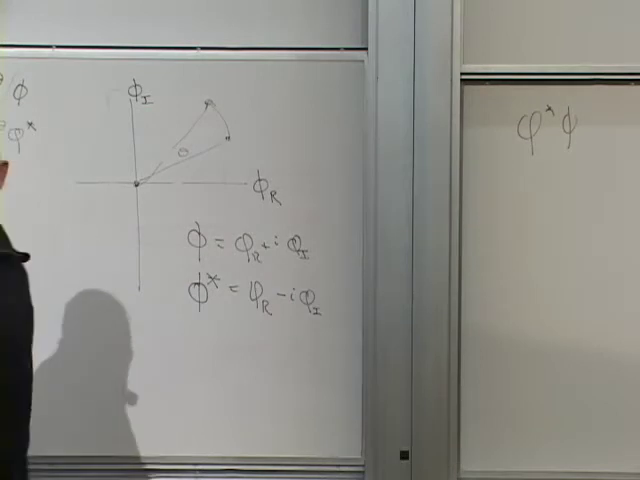
\includegraphics[width=0.80\textwidth]{lecture_07_figure_02.png}
\caption{Комплексное поле на внутренней плоскости \((\phi_R,\phi_I)\). На доске записаны разложения \(\phi\) и \(\phi^*\), а также инвариантный радиус \(\phi^*\phi\).}
\lectureframe{00:33:33}
\end{figure}

Воспользуемся лагранжианом
\begin{equation}
  \mathcal L
  =\partial_\mu\phi^*\,\partial^\mu\phi
   -V(\phi^*\phi).
  \label{eq:l07-complex-lagrangian}
\end{equation}
Для комплексного поля обычный множитель \(1/2\) отсутствует, поскольку этот единственный член уже содержит кинетические члены обеих вещественных компонент. Преобразование
\begin{equation}
  \phi'(x)=e^{i\theta}\phi(x),
  \qquad
  \phi^{*\prime}(x)=e^{-i\theta}\phi^*(x)
  \label{eq:l07-global-u1}
\end{equation}
поворачивает каждое значение поля на один и тот же угол. Здесь \(\theta\) постоянно в пространстве и времени. Штрих обозначает преобразованное поле; это не производная.

Поскольку \(\theta\) постоянно,
\begin{equation}
  \partial_\mu\phi'=e^{i\theta}\partial_\mu\phi,
  \qquad
  \partial_\mu\phi^{*\prime}
  =e^{-i\theta}\partial_\mu\phi^*.
\end{equation}
В кинетическом члене фазы сокращаются, и
\(\phi^{*\prime}\phi'=\phi^*\phi\). Следовательно, любой потенциал, зависящий только от
\(\phi^*\phi\), обладает той же симметрией. Член, зависящий только от \(\phi_R\),
выбирал бы направление во внутренней плоскости и явно нарушал бы симметрию.

\subsection{Точечный минимум и окружность минимумов}

Существуют два качественно различных симметричных потенциала. У первого
единственный минимум находится в начале координат, например
\begin{equation}
  V_{\rm unbroken}=m^2\phi^*\phi,
  \qquad m^2>0.
\end{equation}
Его график представляет собой параболоид с вращательной симметрией. Вакуум \(\phi=0\)
остаётся неизменным при любом повороте, так что симметрия не нарушена.

Теперь выберем
\begin{equation}
  V_{\rm broken}
  =-a\,\phi^*\phi+b(\phi^*\phi)^2,
  \qquad a,b>0.
  \label{eq:l07-mexican-hat}
\end{equation}
Отрицательный квадратичный член уводит поле от начала координат, тогда как
положительный квартичный член не позволяет ему уйти на бесконечность. Обозначив
\(r^2=\phi^*\phi\), из условия минимума получаем
\begin{equation}
  \frac{dV}{d(r^2)}=-a+2br^2=0,
  \qquad
  r^2=f^2=\frac{a}{2b}.
  \label{eq:l07-vacuum-radius}
\end{equation}
Следовательно, минимумы образуют окружность. Потенциал полностью инвариантен относительно
вращений, однако однородное основное состояние должно выбрать одну точку на
этой окружности.

\begin{figure}[htbp]
\centering
\includegraphics[width=0.72\textwidth]{lecture_07_figure_06.png}
\caption{Потенциал, нарушающий симметрию, изображён как поверхность вращения.
Начало координат неустойчиво, а вырожденные минимумы образуют кольцевой жёлоб.}
\lectureframe{00:37:25}
\end{figure}

Представьте поле как маленькую стрелку в этой внутренней плоскости в каждой точке
обычного пространства. Потенциал требует, чтобы каждая стрелка имела длину \(f\). Энергия
градиента требует, чтобы соседние стрелки были направлены почти одинаково.
Поэтому в основном состоянии угол всюду одинаков, но никакой угол не
выделен самим законом. Это и есть непрерывное спонтанное нарушение симметрии.

\section{От доменной стенки к плавному закручиванию}

Повторим граничный эксперимент. На левой границе зафиксируем поле в
вакуумной точке \(A\); на правой зафиксируем его в другой вакуумной точке \(B\). Локализованный
скачок сделал бы градиент большим. Однако, в отличие от дискретного случая,
поле может оставаться на дне потенциала, непрерывно изменяясь по
окружности.

При низкой энергии запишем поле как \(\phi=f e^{i\alpha(x)}\). В одном пространственном
измерении соответствующая энергия равна
\begin{equation}
  E[\alpha]
  =f^2\int_0^L dx\,\left(\frac{d\alpha}{dx}\right)^2.
  \label{eq:l07-angle-functional}
\end{equation}
При фиксированных углах на концах вариация даёт
\begin{equation}
  \frac{d^2\alpha}{dx^2}=0,
  \qquad
  \alpha(x)=\alpha_A+
    \frac{\alpha_B-\alpha_A}{L}\,x.
  \label{eq:l07-linear-twist}
\end{equation}
Предпочтительная конфигурация равномерно распределяет закручивание по всему образцу.
Её энергия масштабируется как
\begin{equation}
  E_{\rm twist}
  =f^2\frac{(\alpha_B-\alpha_A)^2}{L},
  \label{eq:l07-twist-energy}
\end{equation}
так что её можно сделать сколь угодно малой, увеличивая \(L\).

\begin{figure}[htbp]
\centering
\begin{adjustbox}{max width=\linewidth}
\begin{tikzpicture}[x=0.95cm,y=0.95cm]
  \begin{scope}
    \draw[->] (0,0) -- (6.2,0) node[right] {$x$};
    \draw[->] (0,0) -- (0,3.5) node[above] {$\alpha(x)$};
    \draw[very thick,blue!70!black] (0.45,0.65) -- (5.7,2.85);
    \fill (0.45,0.65) circle (1.8pt) node[left] {$\alpha_A$};
    \fill (5.7,2.85) circle (1.8pt) node[right] {$\alpha_B$};
    \node at (3.1,-0.65) {physical space};
  \end{scope}
  \begin{scope}[xshift=9.2cm,yshift=1.65cm]
    \draw[thick] (0,0) circle (1.8);
    \fill (1.55,-0.92) circle (1.8pt) node[below right] {$A$};
    \fill (-0.45,1.74) circle (1.8pt) node[above] {$B$};
    \draw[very thick,blue!70!black,-{Latex[length=2.5mm]}]
      (1.55,-0.92) arc[start angle=-31,end angle=104,radius=1.8];
    \node at (0,-2.35) {vacuum circle};
  \end{scope}
\end{tikzpicture}
\end{adjustbox}
\caption{Одна и та же низкоэнергетическая конфигурация в двух описаниях. Угол
линейно меняется в физическом пространстве, тогда как поле проходит по короткой дуге
вакуумной окружности во внутреннем пространстве.}
\end{figure}

\begin{classroomqa}
\audiencequestion{Вокруг окружности можно пройти двумя путями. По какому пути идёт
поле и может ли оно застрять на более длинном?
\lecturetimestamp{00:41:54}}
\lecturerresponse{Для общих положений концов более короткий угловой путь даёт
меньший градиент и, следовательно, меньшую энергию. Для диаметрально противоположных
концов две простейшие траектории вырождены. Конфигурация, подготовленная
медленным перемещением одного конца, может сохранить лишнюю намотку и оказаться
запертой за энергетическим барьером, но для заданной пары обычных граничных точек
основным состоянием является кратчайший путь без дополнительной намотки.}
\end{classroomqa}

\begin{classroomqa}
\audiencequestion{Может ли траектория уйти с дна жёлоба и срезать через внутреннюю
область, чтобы в целом стать короче?\lecturetimestamp{00:43:32}}
\lecturerresponse{В низкоэнергетическом режиме и для длинного образца невыгодно
подниматься по радиальному потенциалу. Удерживание радиуса на его вакуумном значении и
линейное изменение угла минимизируют эффективную энергию, как показывает
приведённое выше вычисление вариационным исчислением. Для конечной системы с
конкретным потенциалом можно минимизировать радиальное и угловое движение совместно, но
вывод Голдстоуна относится к пределу сколь угодно большой длины волны, в котором
выигрывает гладкое движение вдоль жёлоба.}
\end{classroomqa}

\begin{classroomqa}
\audiencequestion{Что изменится, если кольцевой жёлоб наклонить так, что одно
значение угла окажется ниже?\lecturetimestamp{00:44:33}}
\lecturerresponse{Тогда симметрия явно нарушена. Одна точка становится
истинным основным состоянием, движение вдоль окружности приобретает возвращающую силу,
и угловое возбуждение уже не является точно безмассовым.}
\end{classroomqa}

\section{Масса как цена колебания с нулевым импульсом}

Плавное закручивание выявляет поле, энергия которого обусловлена только градиентами. Чтобы
понять, почему это означает безмассовую частицу, сравним релятивистское
дисперсионное соотношение
\begin{equation}
  \omega^2=\bm{k}^2+m^2.
  \label{eq:l07-dispersion}
\end{equation}
Волна \(e^{i(\bm{k}\cdot\bm{x}-\omega t)}\) несёт импульс \(\bm{k}\).
Если \(m=0\), её энергия стремится к нулю, когда длина волны стремится к бесконечности:
\(\omega=|\bm{k}|\to0\). Если \(m\ne0\), то пространственно однородная мода
\(\bm{k}=0\) всё же осциллирует с частотой \(\omega=m\). Масса — это
неустранимая энергия при нулевом импульсе.

То же различие видно и в лагранжиане. Член
\begin{equation}
  -\frac12m^2\varphi^2
\end{equation}
создаёт возвращающую силу даже для однородного смещения. У поля, содержащего
только производные члены, такой возвращающей силы нет: увеличивайте его длину волны,
и его градиентная энергия стремится к нулю.

\subsection{Полярные переменные разделяют две моды}

Запишем комплексное поле в нарушенной фазе как
\begin{equation}
  \phi(x)=\rho(x)e^{i\alpha(x)}.
  \label{eq:l07-polar}
\end{equation}
И \(\rho\), и \(\alpha\) являются полями. Дифференцирование даёт
\begin{align}
  \partial_\mu\phi
  &=e^{i\alpha}
    \left(\partial_\mu\rho+i\rho\,\partial_\mu\alpha\right),\\
  \partial_\mu\phi^*
  &=e^{-i\alpha}
    \left(\partial_\mu\rho-i\rho\,\partial_\mu\alpha\right).
\end{align}
Перекрёстные члены сокращаются, и остаётся
\begin{equation}
  \partial_\mu\phi^*\,\partial^\mu\phi
  =(\partial_\mu\rho)(\partial^\mu\rho)
   +\rho^2(\partial_\mu\alpha)(\partial^\mu\alpha).
  \label{eq:l07-polar-kinetic}
\end{equation}
Поскольку \(\phi^*\phi=\rho^2\),
\begin{equation}
  \mathcal L
  =(\partial\rho)^2+\rho^2(\partial\alpha)^2-V(\rho^2).
  \label{eq:l07-polar-lagrangian}
\end{equation}
Потенциал содержит \(\rho\), но не \(\alpha\). Это отсутствие и есть
симметрия в её наиболее полезной форме.

\begin{figure}[htbp]
\centering
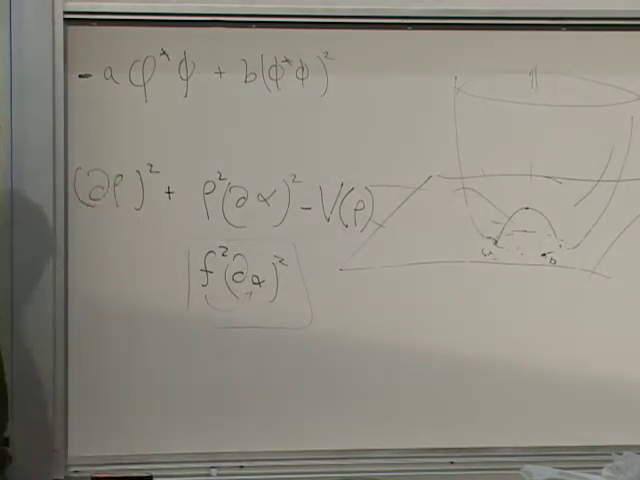
\includegraphics[width=0.88\textwidth]{lecture_07_figure_03.png}
\caption{Лагранжиан поля в полярных переменных, выделенный рамкой низкоэнергетический угловой член и
потенциал, нарушающий симметрию. Радиальное движение поднимается по потенциалу; угловое
движение идёт вдоль жёлоба.}
\lectureframe{00:56:40}
\end{figure}

Для возбуждения с очень малой энергией поле остаётся близким к
\(\rho=f\). Тогда
\begin{equation}
  \mathcal L_{\rm angular}
  \simeq f^2(\partial_\mu\alpha)(\partial^\mu\alpha).
\end{equation}
Определим канонически нормированное угловое поле, с точностью до соглашения о множителях \(1/2\), как
\begin{equation}
  \beta=\sqrt{2}\,f\alpha,
  \qquad
  \mathcal L_{\rm angular}
  =\frac12(\partial_\mu\beta)(\partial^\mu\beta).
  \label{eq:l07-goldstone-field}
\end{equation}
Члена \(\beta^2\) нет. Кванты этого углового поля безмассовы.
Это бозоны Голдстоуна.

Радиальное поле ведёт себя иначе. Если сразу всюду сместить \(\rho\) от \(f\),
оно скатится обратно, пройдёт через минимум и будет осциллировать около жёлоба. Если
\(\rho=f+h\), то разложение формулы ~\eqref{eq:l07-mexican-hat} даёт
\begin{equation}
  V(f+h)=V(f)+\frac12m_h^2h^2+\cdots,
\end{equation}
так что \(h\) имеет массу. Геометрически угловое направление плоское, а
радиальное — искривлённое.

\begin{classroomqa}
\audiencequestion{Если поле смещено радиально, просто ли оно падает
обратно вниз и что происходит потом?\lecturetimestamp{00:57:10}}
\lecturerresponse{Если углового движения нет, оно падает к минимуму,
проходит через него и осциллирует радиально. Однородное колебание имеет нулевой
пространственный импульс, но ненулевую частоту; эта частота и есть масса
радиального возбуждения. Однородное угловое смещение, напротив, приводит к
другому вакууму и не имеет возвращающей силы.}
\end{classroomqa}

В рассматриваемом примере содержание принципа Голдстоуна таково:
спонтанное нарушение непрерывной глобальной симметрии порождает безмассовую моду
для каждого независимого плоского направления многообразия вакуума.
\editorialnote{Это утверждение предполагает обычные условия релятивистской
теории поля. В нерелятивистских многочастичных системах подсчёт и
дисперсия мод Намбу--Голдстоуна могут быть более тонкими, но вывод лекции о
длинноволновом пределе остаётся верным для этой релятивистской модели \(U(1)\).}

\section{Спиновые волны, струны и звук}

Теорема абстрактна, но её механизм хорошо знаком. В изотропном
ферромагните все спины можно повернуть совместно, не изменяя энергии.
Если позволить ориентации очень медленно меняться по образцу, получится
спиновая волна. Её энергетическая цена обращается в нуль вместе с её волновым
числом, так что это мода Голдстоуна нарушенной симметрии вращения спинов.

Длинная упругая струна даёт другую наглядную картину. Пренебрежём гравитацией и закрепим
концы так, чтобы всю струну можно было сдвигать по вертикали. Однородный
вертикальный сдвиг не требует энергии. Если позволить ему медленно меняться вдоль
струны, он превращается в длинноволновую поперечную волну. Однородная
операция симметрии превращена в плавную деформацию, зависящую от
положения.

\begin{figure}[htbp]
\centering
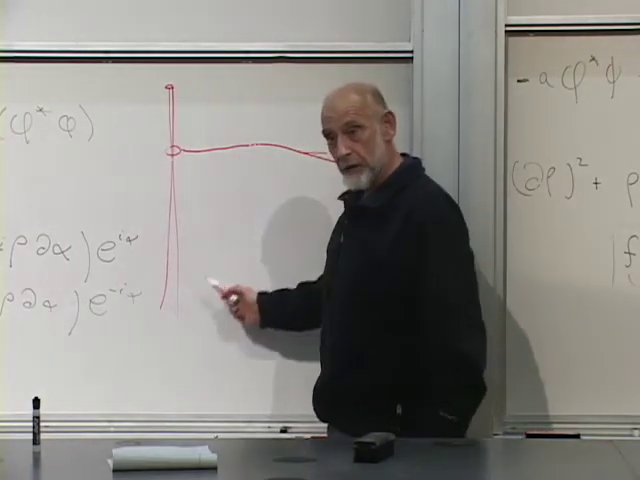
\includegraphics[width=0.68\textwidth]{lecture_07_figure_04.png}
\caption{Медленно меняющийся профиль струны, нарисованный при аналогии с модой Голдстоуна.
Физически важен малый наклон длинноволновой деформации, а не вертикальное положение
кривой.}
\lectureframe{01:04:19}
\end{figure}

\begin{classroomqa}
\audiencequestion{Может ли струна нести энергию колебаний, имея при этом нулевой
импульс?\lecturetimestamp{01:04:41}}
\lecturerresponse{Нужно различать вертикальный механический импульс и
волновой импульс вдоль струны. Стоячая волна может иметь нулевой суммарный импульс,
поскольку она является суперпозицией мод с \(+k\) и \(-k\), и при этом всё же
нести энергию. В аналогии с теорией поля импульс относится к волновому
числу вдоль оси; вертикальное смещение представляет внутреннюю координату
поля.}
\end{classroomqa}

Пружинка-слинки дает продольный аналог. Сдвиньте всю идеализированную бесконечную пружинку вдоль ее оси — и ничего не изменится. Сдвиньте соседние части на немного разные величины — и получится слабая волна сжатия. В твердом теле или жидкости длинноволновой звук аналогично возникает из коллективных смещений и изменений плотности. Спиновые волны, поперечные волны на струне и звук — не одно и то же микроскопическое возбуждение, но у них есть решающая общая черта: однородное непрерывное преобразование не требует энергии, а его медленно меняющийся вариант становится мягкой модой.
\editorialnote{В кристалле акустические фононы обычно описывают как моды Намбу--Голдстоуна, возникающие при спонтанном нарушении непрерывных трансляций. Струна и пружинка-слинки — механические аналогии, используемые в лекции, чтобы выявить ту же структуру энергии, зависящую только от производных.}

Терминология здесь достаточно важна, чтобы позволить себе короткую шутку в аудитории: это \emph{Голдстоуна}-бозоны, названные в честь Джеффри Голдстоуна, а не калибровочные бозоны. В лекции отмечается, что Голдстоун был другом Сасскинда, после чего изложение переходит к действительно другой теме — калибровочной инвариантности.

\section{От глобальной фазовой симметрии к калибровочной симметрии}

Симметрия фаз \(U(1)\) уже появлялась в курсе как симметрия, связанная с сохранением заряда. Поля заряженных частиц комплексны, и умножение такого поля на общую фазу оставляет глобальную теорию неизменной. Для наглядности можно говорить об электрическом заряде, хотя он может представлять и другое квантовое число \(U(1)\). Настоящий фотон безмассов; конечная цель — фотоноподобное поле, такое как массивное \(Z\).

Новый вопрос состоит в том, может ли
\begin{equation}
  \phi'(x)=e^{i\theta(x)}\phi(x)
  \label{eq:l07-local-u1}
\end{equation}
быть симметрией, когда \(\theta\) произвольно меняется в пространстве-времени. Функция \(\theta(x)\) — это параметр преобразования, а не дополнительное динамическое поле. Проверим это предложение, продифференцировав:
\begin{equation}
  \partial_\mu\phi'
  =e^{i\theta}
   \left[\partial_\mu\phi+i(\partial_\mu\theta)\phi\right].
  \label{eq:l07-local-derivative}
\end{equation}
Этот дополнительный член отсутствовал при постоянной \(\theta\). Для комплексно-сопряженного поля
\begin{equation}
  \partial_\mu\phi^{*\prime}
  =e^{-i\theta}
   \left[\partial_\mu\phi^*-i(\partial_\mu\theta)\phi^*\right].
\end{equation}
Их произведение равно
\begin{align}
  \partial_\mu\phi^{*\prime}\partial^\mu\phi'
  ={}&
  \partial_\mu\phi^*\partial^\mu\phi
  i\left(
      \phi\,\partial_\mu\phi^*
      -\phi^*\partial_\mu\phi
    \right)\partial^\mu\theta
  \nonumber\\
  &+\phi^*\phi\,
    \partial_\mu\theta\,\partial^\mu\theta.
  \label{eq:l07-local-failure}
\end{align}
Потенциал остается инвариантным, потому что инвариантно \(\phi^*\phi\), но обычный кинетический член перестает быть инвариантным. Глобальная симметрия не стала автоматически локальной.

\begin{classroomqa}
\audiencequestion{На картинке с «мексиканской шляпой» означает ли эта неудача, что вдоль кругового желоба есть бугорки?\lecturetimestamp{01:19:37}}
\lecturerresponse{Нет. Потенциал может оставаться совершенно плоским в угловом направлении. Дополнительная энергетическая цена возникает из-за градиентов, когда фаза различается от одной точки пространства-времени к другой. Это не гофрировка желоба; это обычный член с производной, который обнаруживает пространственную неоднородность.}
\end{classroomqa}

\subsection{Компенсирующее векторное поле}

В природе взаимодействия фотона, \(W\), \(Z\) и глюонов организованы локальными калибровочными симметриями, а не просто жесткими преобразованиями. Чтобы локальная фазовая операция стала симметрией, нужно расширить теорию, введя четырехвекторное поле \(A_\mu\). В электромагнетизме \(A_0\) — скалярный потенциал, а три пространственные компоненты образуют векторный потенциал. Из их производных строятся электрическое и магнитное поля.

Выберите внутренне согласованное соглашение
\begin{equation}
  \phi'=e^{i\theta}\phi,
  \qquad
  A'_\mu=A_\mu-\partial_\mu\theta,
  \qquad
  D_\mu=\partial_\mu+iA_\mu.
  \label{eq:l07-gauge-convention}
\end{equation}
На доске при проверке компенсации меняется знак; уравнение
\eqref{eq:l07-gauge-convention} одновременно фиксирует все три знака. Константа калибровочного
взаимодействия и заряд временно поглощены в \(A_\mu\).
\editorialnote{При явном указании заряда \(q\) и константы связи \(g\) можно записать
\(D_\mu=\partial_\mu+igqA_\mu\) и
\(A'_\mu=A_\mu-(gq)^{-1}\partial_\mu\theta\). На лекции эти
константы опущены, чтобы компенсация оставалась наглядной.}

Для сопряжённого поля
\begin{equation}
  D_\mu\phi^*=\partial_\mu\phi^*-iA_\mu\phi^*.
\end{equation}
Теперь
\begin{align}
  D'_\mu\phi'
  &=
  \left(\partial_\mu+iA'_\mu\right)e^{i\theta}\phi
  \nonumber\\
  &=
  e^{i\theta}
  \left[
    \partial_\mu\phi+i(\partial_\mu\theta)\phi
    +i(A_\mu-\partial_\mu\theta)\phi
  \right]
  \nonumber\\
  &=e^{i\theta}D_\mu\phi.
  \label{eq:l07-covariant-transform}
\end{align}
Нежелательная производная от \(\theta\) компенсируется преобразованием
\(A_\mu\). Аналогично,
\begin{equation}
  D'_\mu\phi^{*\prime}=e^{-i\theta}D_\mu\phi^*.
\end{equation}
Их произведение инвариантно. Прилагательное \emph{ковариантная} означает, что
производная преобразуется тем же простым образом, что и само поле.

\section{Динамика калибровочного поля}

Введение \(A_\mu\) лишь для исправления производной оставило бы его без
собственной динамики. Калибровочно-инвариантная напряжённость поля равна
\begin{equation}
  F_{\mu\nu}
  =\partial_\mu A_\nu-\partial_\nu A_\mu.
  \label{eq:l07-field-strength}
\end{equation}
Она антисимметрична, поэтому \(F_{\mu\mu}=0\).

Её время--пространственные компоненты содержат
электрическое поле, тогда как пространство--пространственные компоненты содержат магнитное
поле. В привычных обозначениях с трёхмерными векторами плотность энергии
электромагнитного поля пропорциональна \(\bm E^2+\bm B^2\), тогда как лоренцев лагранжиан
пропорционален \(\bm E^2-\bm B^2\); знаки зависят от принятого соглашения
о метрике.

\begin{classroomqa}
\audiencequestion{Каковы энергия и лагранжиан электромагнитного
поля?\lecturetimestamp{01:33:20}}
\lecturerresponse{Энергия строится из \(E^2+B^2\); в лагранжиане используется
\(E^2-B^2\). В ковариантной форме последняя величина записывается как
\(F_{\mu\nu}F^{\mu\nu}\), умноженное на стандартный коэффициент. Антисимметричный тензор — это четырёхмерный
ротор векторного потенциала.}
\end{classroomqa}

Напряжённость поля сама по себе калибровочно-инвариантна:
\begin{align}
  F'_{\mu\nu}
  &=
  \partial_\mu(A_\nu-\partial_\nu\theta)
  -\partial_\nu(A_\mu-\partial_\mu\theta)
  \nonumber\\
  &=
  F_{\mu\nu}
  -\partial_\mu\partial_\nu\theta
  +\partial_\nu\partial_\mu\theta
  =F_{\mu\nu}.
  \label{eq:l07-field-strength-invariant}
\end{align}
Последнее равенство следует из того, что обычные смешанные частные производные
коммутируют. Поэтому стандартный калибровочно-инвариантный лагранжиан имеет вид
\begin{equation}
  \boxed{
  \mathcal L
  =(D_\mu\phi)^*D^\mu\phi
  -V(\phi^*\phi)
  -\frac14F_{\mu\nu}F^{\mu\nu}}
  \label{eq:l07-scalar-qed}
\end{equation}
с точностью до соглашений о знаках и нормировке, выбранных для метрики.

\begin{figure}[htbp]
\centering
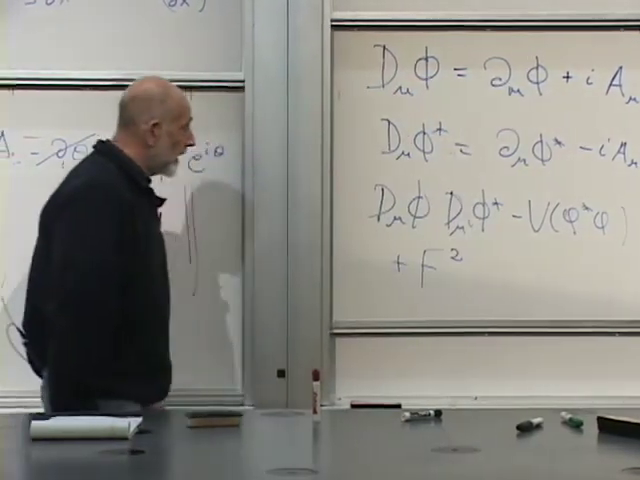
\includegraphics[width=0.84\textwidth]{lecture_07_figure_05.png}
\caption{Ковариантные производные и построенный на доске калибровочно-инвариантный
лагранжиан. Численные множители там опущены, чтобы структура
преобразований оставалась наглядной.}
\lectureframe{01:38:45}
\end{figure}

Эта конструкция повышает глобальную симметрию \(U(1)\) до локальной, но делает это ценой --- или, физически говоря, даруя нам --- новое векторное поле.
В абелевом примере этим полем является электромагнитный потенциал.

\begin{classroomqa}
\audiencequestion{Лагранжиан, с которого мы начали, использовал обычные производные. Почему
мы вправе заменить их ковариантными производными и назвать результат
настоящей теорией?\lecturetimestamp{01:42:55}}
\lecturerresponse{Мы строим другую, расширенную теорию: заряженная
материя плюс калибровочное поле. Локальная калибровочная инвариантность определяет их взаимодействие.
Получающаяся квантовая теория представляет собой согласованную математическую структуру и согласуется
с тем, как природа организует фотон и слабые калибровочные поля. Простое несогласованное введение
взаимодействия релятивистского векторного поля может привести к нефизическим
поляризациям и нарушениям вероятностной интерпретации, так что калибровочный принцип не является
косметической перезаписью старой теории свободного скалярного поля.}
\end{classroomqa}

\begin{classroomqa}
\audiencequestion{То есть добавление нового поля и есть главное обоснование этой модификации?\lecturetimestamp{01:44:57}}
\lecturerresponse{Да. Без \(A_\mu\) производная локально повернутого поля содержит нескомпенсированный \(\partial_\mu\theta\). При наличии \(A_\mu\) и закона его преобразования сокращение происходит. На геометрическом языке \(A_\mu\) — это связность на расслоении; эта более глубокая математика вполне реальна и полезна, но приведенная выше алгебра содержит ту часть, которая здесь нужна.}
\end{classroomqa}

\section{Почему запрещена затравочная масса калибровочного бозона}

Для обычного бозонного поля масса представляется квадратичным членом.
Естественно попытаться добавить
\begin{equation}
  \Delta\mathcal L_{\rm Proca}
  =\frac12m^2A_\mu A^\mu.
  \label{eq:l07-proca}
\end{equation}
Однако при \(A_\mu\mapsto A_\mu-\partial_\mu\theta\)
\begin{equation}
  A'_\mu A^{\mu\prime}
  =
  A_\mu A^\mu
  -2A^\mu\partial_\mu\theta
  +\partial_\mu\theta\,\partial^\mu\theta,
\end{equation}
поэтому формула~\eqref{eq:l07-proca} не является калибровочно-инвариантной. Мы не можем ввести массу в эту калибровочную теорию вручную, сохранив ее локальную симметрию.

\begin{figure}[htbp]
\centering
\includegraphics[width=0.72\textwidth]{lecture_07_figure_07.png}
\caption{Предлагаемый затравочный массовый член для векторного поля
\(\tfrac12m^2A_\mu A^\mu\). Именно то, что он неинвариантен при
\(A_\mu\mapsto A_\mu-\partial_\mu\theta\), и создает препятствие, ведущее к
механизму Хиггса.}
\lectureframe{01:39:48}
\end{figure}

В этом и состоит кажущийся тупик. Калибровочная инвариантность объясняет, почему фотон безмассов, и защищает теорию от нефизических степеней свободы, но \(W\) и
\(Z\) массивны. Выходом не может быть явная масса векторного поля. Она должна
возникать из полей, уже присутствующих в калибровочно-инвариантном лагранжиане.

\begin{classroomqa}
\audiencequestion{Само введение калибровочной инвариантности порождает
бозон Голдстоуна?\lecturetimestamp{01:45:51}}
\lecturerresponse{Нет. Бозон Голдстоуна возник, когда непрерывная
\emph{глобальная} симметрия была спонтанно нарушена, еще до введения векторного потенциала.
Как только симметрия становится локальной, изменяющуюся фазу можно
скомпенсировать с помощью \(A_\mu\). В калибровочной теории с нарушенной симметрией угловая мода больше
не является независимой безмассовой частицей; она обеспечивает дополнительную
поляризацию теперь уже массивного векторного поля. На следующей лекции это утверждение будет выведено,
а не просто объявлено.}
\end{classroomqa}

\begin{classroomqa}
\audiencequestion{Объясняет ли что-то из этого, почему реки меандрируют?
\lecturetimestamp{01:47:03}}
\lecturerresponse{О прямой связи здесь ничего не известно. Вихри в жидкости и даже
формы организмов, разумеется, можно описывать методами симметрии,
и не стоит удивляться, если идеи теории поля обнаруживаются в неожиданных
местах, но лекция не утверждает существования калибровочной теории речных меандров.}
\end{classroomqa}

\section{На этом лекция заканчивается}

Теперь у нас есть две составляющие, обещанные в начале. Непрерывная
глобальная симметрия, у которой вакуумы образуют окружность, имеет плоское угловое направление, и медленное
изменение вдоль него представляет собой безмассовое поле Голдстоуна. Локальная симметрия требует калибровочной
связности и ковариантных производных и запрещает прямую массу векторного
поля в формуле~\eqref{eq:l07-proca}.

Следующий шаг — использовать потенциал с нарушенной симметрией из уравнения~\eqref{eq:l07-mexican-hat} в калибровочно-инвариантной теории из уравнения~\eqref{eq:l07-scalar-qed}. Тогда одновременно происходят две вещи: отдельная частица Голдстоуна исчезает из физического спектра, а векторное поле приобретает массу. В обычном учебном изложении говорят, что калибровочная симметрия спонтанно нарушается; точнее, калибровочная избыточность сохраняется, а теория входит в фазу Хиггса с массивным векторным возбуждением.
\editorialnote{Локальная калибровочная симметрия — это избыточность описания, а не обычная физическая симметрия, действующая между различными наблюдаемыми состояниями. В лекции используется стандартное сокращённое выражение о спонтанном нарушении калибровочной симметрии. Калибровочно-инвариантное физическое утверждение — это перестройка степеней свободы в фазе Хиггса.}

Это и есть явление Хиггса. Мы его ещё не осуществили. В этой лекции была проделана необходимая, более трудная работа: задача сформулирована достаточно точно, так что её решение, когда оно появится, окажется неизбежным.

\chapter{Механизм Хиггса: как калибровочный бозон приобретает массу}

Теперь мы соединяем две идеи, развитые в предыдущей лекции. Комплексное скалярное поле с нарушенной глобальной симметрией \(U(1)\) содержит массивное радиальное колебание и безмассовое угловое колебание. Локально инвариантная теория \(U(1)\) содержит безмассовое калибровочное поле. Когда скалярное поле заряжено и его равновесный модуль ненулевой, эти утверждения нельзя просто сложить вместе. Угловая мода и калибровочное поле объединяются: калибровочное поле становится массивным, кажущийся бозон Голдстоуна перестает быть независимой частицей, а радиальная хиггсовская мода остается.

Фотон послужит нам модельным калибровочным бозоном, но не тем физическим результатом, к которому мы придем. Электромагнитная \(U(1)\) не нарушена в вакууме, поэтому реальный фотон безмассов. Тот же механизм действует на \(W^\pm\) и \(Z\) в электрослабой теории, где калибровочная группа и скалярный мультиплет устроены сложнее. Абелева модель показывает механизм, не скрывая его за групповой теорией.

\begin{classroomqa}\audiencequestion{Означало ли предыдущее обсуждение, что механизм Хиггса сообщает массу реальному фотону?\lecturetimestamp{00:00:23}}\lecturerresponse{Нет. Мы спрашиваем, что произошло бы \emph{если} бы связанная с фотоном симметрия \(U(1)\) находилась в нарушенной фазе. Такой гипотетический фотон стал бы массивным. Реальный электромагнитный вакуум не находится в этой фазе; в физике элементарных частиц речь вместо этого идет о массе \(W\) и \(Z\).}\end{classroomqa}

Симметрия, связанная с сохранением электрического заряда, — это фазовое вращение \begin{equation}
  \phi(x)\longmapsto e^{i\theta}\phi(x),
\end{equation} внутреннее вращение, называемое \(U(1)\). Сверхпроводник дает реальный аналог нарушенной фазы. Внутри него электромагнитное поле имеет конечную глубину проникновения и в важных отношениях ведет себя как массивное поле. Вне него вновь появляется обычный безмассовый фотон.

\section{Что означает масса для поля}

\subsection{Дисперсия и щель при нулевом импульсе}

Прежде чем вводить поле Хиггса, полезно точно определить, что мы понимаем под массой. Для волны \begin{equation}
  E=\hbar\omega,
  \qquad
  p=\hbar k,
  \label{eq:l08-quantum-wave}
\end{equation} поэтому график \((E,p)\) и график \((\omega,k)\) содержат одну и ту же информацию с точностью до множителей \(\hbar\). В пустом пространстве безмассовое релятивистское возбуждение подчиняется \begin{equation}
  E=c|p|,
  \qquad
  \omega=c|k|.
  \label{eq:l08-massless-dispersion}
\end{equation} Два знака \(k\) соответствуют противоположным направлениям распространения. Существенный момент состоит в том, что \(\omega\) стремится к нулю, когда \(k\) стремится к нулю.

Массивная релятивистская частица подчиняется \begin{equation}
  E^2=c^2p^2+m^2c^4.
  \label{eq:l08-massive-dispersion}
\end{equation} В единицах \(c=\hbar=1\) получаем \begin{equation}
  \omega^2=k^2+m^2.
\end{equation} При \(k=0\) энергия равна \(E=mc^2\), или просто \(m\) в естественных единицах. Следовательно, масса — это ненулевая энергетическая щель моды с нулевым импульсом.

\begin{figure}[htbp]\centering
\begin{adjustbox}{max width=\linewidth}\begin{tikzpicture}[x=1.05cm,y=1.05cm]
  \begin{scope}
    \draw[->] (-0.2,0) -- (4.2,0) node[right] {\(k\)};
    \draw[->] (0,-0.2) -- (0,3.1) node[above] {\(\omega\)};
    \draw[very thick,blue!65!black] (0,0) -- (3.8,2.75);
    \draw[very thick,orange!70!black] (0,0) -- (3.8,1.75);
    \node[blue!65!black,rotate=36] at (2.65,2.15)
      {\(\omega=c_{\rm vac}k\)};
    \node[orange!70!black,rotate=24] at (2.65,1.05)
      {ordinary medium};
    \node[below] at (2,-0.45) {gapless};
  \end{scope}
  \begin{scope}[xshift=6.2cm]
    \draw[->] (-0.2,0) -- (4.2,0) node[right] {\(k\)};
    \draw[->] (0,-0.2) -- (0,3.1) node[above] {\(\omega\)};
    \draw[very thick,domain=0:3.8,samples=120,smooth,teal!70!black]
      plot (\x,{sqrt(0.9+0.45*\x*\x)});
    \draw[dashed] (0,0.95) -- (1.0,0.95);
    \node[left] at (0,0.95) {\(m\)};
    \node[teal!70!black] at (2.55,2.15)
      {\(\omega^2=k^2+m^2\)};
    \node[below] at (2,-0.45) {gapped};
  \end{scope}
\end{tikzpicture}\end{adjustbox}\caption{Изменение скорости распространения меняет наклон бесщелевого дисперсионного соотношения. Придание возбуждению массы открывает ненулевую щель при \(k=0\).}\label{fig:l08-dispersion}\end{figure}

Обычная прозрачная среда может уменьшать фазовую скорость волны, не создавая при этом такой релятивистской массовой щели. На границе частота падающей волны фиксирована, тогда как волновое число подстраивается под дисперсионное соотношение среды. Изменение наклона — не то же самое, что смещение вверх точки пересечения с осью ординат. \editorialnote{Среда может иметь несколько электромагнитных ветвей, а плазма или резонансная среда могут обладать ненулевой плазменной частотной щелью. В лекции сравнение проводится именно между обычной преломляющей ветвью и сверхпроводящим откликом. В более общем смысле бесщелевость означает \(\omega(k)\to0\) при \(k\to0\); точная линейность требуется не во всякой нерелятивистской среде.}

\begin{classroomqa}\audiencequestion{Приобретает ли фотон массу всякий раз, когда проходит через вещество, например через призму?\lecturetimestamp{00:03:02}}\lecturerresponse{Нет. Преломление может изменить связь между частотой и волновым числом, а значит и скорость распространения, при этом ветвь по-прежнему проходит через \(\omega=0\) при \(k=0\). Сверхпроводящая фаза, напротив, придает электромагнитному отклику конечную обратную длину проникновения, аналог массы.}\end{classroomqa}

\begin{classroomqa}\audiencequestion{Если свет фиксированной частоты входит в стекло, меняется ли именно волновое число?\lecturetimestamp{00:09:20}}\lecturerresponse{Да. Инвариантность относительно сдвигов по времени на стационарной границе сохраняет частоту фиксированной. Поскольку дисперсионная кривая в стекле имеет другой наклон, одному и тому же \(\omega\) соответствует другое \(k\) и, следовательно, другая длина волны.}\end{classroomqa}

Наклон \begin{equation}
  v_g=\frac{d\omega}{dk}
\end{equation} есть групповая скорость волнового пакета. Если этот наклон зависит от \(k\), разные фурье-компоненты движутся с разными скоростями, и пакет расплывается. Поэтому зависимость \(\omega(k)\) называется \emph{дисперсионным соотношением}.

\begin{classroomqa}\audiencequestion{Как называется эта кривая и что означает ее наклон?\lecturetimestamp{00:11:02}}\lecturerresponse{Эта кривая — дисперсионное соотношение. Ее производная \(d\omega/dk\) есть групповая скорость. Постоянный наклон дает одну и ту же скорость всем длинам волн; меняющийся наклон заставляет волновой пакет расплываться. Для нашей цели решающее различие состоит в том, достигает ли кривая начала координат или имеет щель.}\end{classroomqa}

\subsection{Однородное колебание — это частица в покое}

Мода \(k=0\) имеет бесконечную длину волны: поле смещено на одну и ту же величину всюду. Отпустим такое однородное смещение. Если поле колеблется с ненулевой частотой, соответствующий квант имеет ненулевую энергию покоя и является массивным. Если в этом направлении нет восстанавливающей силы, частота обращается в нуль, и мода безмассовая.

Это утверждение классическое. Оно не требует, чтобы пространственно разделенные частицы находились в квантовой суперпозиции. Однородная конфигурация классического поля — это просто одно и то же значение поля, повторяющееся по всему пространству.

\begin{classroomqa}\audiencequestion{Если все поле сдвигается целиком, то это то же самое, что квантовая запутанность?\lecturetimestamp{00:10:04}}\lecturerresponse{Нет. Однородное классическое поле — это одна классическая конфигурация. Запутанность коррелирует различные квантовые альтернативы, например конфигурации спинов вверх--вниз и вниз--вверх. Задание одного и того же значения поля во многих точках само по себе не является запутанностью и не подразумевает мгновенного причинного отклика.}\end{classroomqa}

Для канонически нормированного действительного поля \begin{equation}
  \mathcal L
  =\frac12\partial_\mu\varphi\,\partial^\mu\varphi-V(\varphi),
\end{equation} разложим около равновесного значения \(\varphi_0\): \begin{equation}
  V(\varphi_0+\eta)
  =V(\varphi_0)
   +\frac12V''(\varphi_0)\eta^2+\cdots.
\end{equation} Линейный член в минимуме исчезает, и уравнение поля дает \begin{equation}
  \omega^2=\bm{k}^2+m^2,
  \qquad
  m^2=V''(\varphi_0).
  \label{eq:l08-curvature-mass}
\end{equation} Следовательно, масса — это кривизна потенциала в направлении движения. Плоское направление имеет нулевую кривизну и дает безмассовую моду.

\section{Комплексное скалярное поле с нарушенной симметрией}

\subsection{Радиальное и угловое движение}

Запишем комплексное скалярное поле в декартовых и полярных координатах: \begin{equation}
  \phi=\phi_R+i\phi_I=\rho e^{i\alpha},
  \qquad
  \phi^*=\phi_R-i\phi_I=\rho e^{-i\alpha}.
  \label{eq:l08-polar-field}
\end{equation} Комплексная плоскость — это \emph{внутреннее} пространство поля. В каждой физической точке пространства-времени \(x\) пара \((\phi_R(x),\phi_I(x))\) задает одну точку на этой внутренней плоскости. Ни одна из внутренних осей не является направлением в лаборатории.

\begin{figure}[htbp]\centering
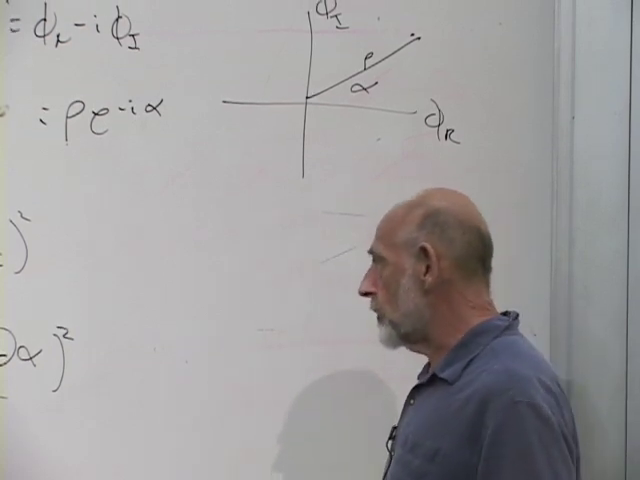
\includegraphics[width=0.72\textwidth]{lecture_08_figure_02.png}\caption{Комплексное скалярное поле, представленное на своей внутренней плоскости \((\phi_R,\phi_I)\). Радиус равен \(\rho\), а \(\alpha\) — внутренняя фаза.}\lectureframe{00:24:41}\label{fig:l08-internal-plane}\end{figure}

Кинетический член скалярного поля принимает вид \begin{align}
  \partial_\mu\phi^*\,\partial^\mu\phi
  &=
  \partial_\mu\phi_R\,\partial^\mu\phi_R
  +\partial_\mu\phi_I\,\partial^\mu\phi_I
  \notag\\
  &=
  \partial_\mu\rho\,\partial^\mu\rho
  +\rho^2\partial_\mu\alpha\,\partial^\mu\alpha.
  \label{eq:l08-polar-kinetic}
\end{align} Глобально \(U(1)\)-инвариантный потенциал зависит от \(\phi^*\phi=\rho^2\), а не от \(\alpha\). Например, \begin{equation}
  V(\phi)
  =\lambda\left(\phi^*\phi-\frac{f^2}{2}\right)^2,
  \qquad \lambda>0.
  \label{eq:l08-mexican-hat}
\end{equation} Его минимумы образуют окружность. Закон инвариантен относительно общего фазового поворота, но выбор одной равновесной фазы выделяет одну точку на окружности.

\begin{figure}[htbp]\centering
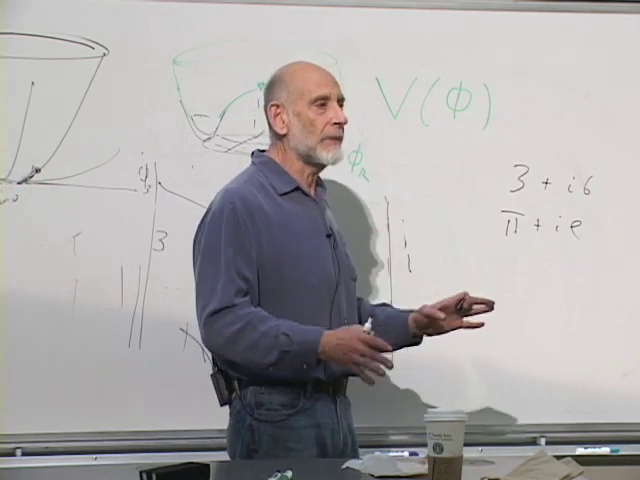
\includegraphics[width=0.78\textwidth]{lecture_08_figure_03.png}\caption{Наброски радиального потенциала на доске. Потенциал симметричен относительно вращений значения поля во внутреннем пространстве, хотя самому полю не обязательно находиться в начале координат.}\lectureframe{00:34:22}\label{fig:l08-radial-potential-board}\end{figure}

\begin{figure}[htbp]\centering
\begin{tikzpicture}[x=0.94cm,y=0.94cm]
  \draw[->] (-4.2,0) -- (4.4,0) node[right] {\(\phi_R\)};
  \draw[->] (0,-3.7) -- (0,3.9) node[above] {\(\phi_I\)};
  \draw[very thick,blue!65!black] (0,0) circle (2.45);
  \draw[->,very thick,orange!75!black] (0,0) -- (2.2,1.08);
  \draw[->,very thick,teal!70!black]
    (2.2,1.08) arc[start angle=26,end angle=67,radius=2.45];
  \node[orange!75!black,below right] at (1.15,0.52)
    {radial \(h\): massive};
  \node[teal!70!black,above right] at (1.78,1.76)
    {angular \(\pi\): massless};
  \fill (2.2,1.08) circle (2pt);
  \node[below] at (0,-2.65) {degenerate vacuum circle};
\end{tikzpicture}\caption{В глобальной теории с нарушенной симметрией есть кривизна по нормали к вакуумной окружности, но нет кривизны вдоль нее. Радиальная хиггсовская мода массивна; угловая голдстоуновская мода безмассовая.}\label{fig:l08-radial-angular}\end{figure}

Положим \begin{equation}
  \phi(x)=\frac{f+h(x)}{\sqrt2}
           e^{i\pi(x)/f}.
  \label{eq:l08-canonical-polar}
\end{equation} Вблизи выбранного вакуума \(h\) описывает радиальное смещение, а \(\pi\) — тангенциальное смещение с каноническими размерностями. Подстановка в ур.~\eqref{eq:l08-polar-kinetic} дает \begin{equation}
  \partial_\mu\phi^*\,\partial^\mu\phi
  =
  \frac12(\partial_\mu h)^2
  +\frac12\left(1+\frac{h}{f}\right)^2
            (\partial_\mu\pi)^2.
  \label{eq:l08-global-expanded}
\end{equation} Потенциал в ур.~\eqref{eq:l08-mexican-hat} дает \begin{equation}
  m_h^2=2\lambda f^2,
  \qquad
  m_\pi^2=0.
  \label{eq:l08-global-masses}
\end{equation} При энергиях, много меньших, чем \(m_h\), радиальное движение требует больших затрат энергии, поэтому можно временно зафиксировать \(h=0\). Оставшийся лагранжиан содержит только \(\frac12(\partial\pi)^2\), без члена \(\pi^2\). Это и есть бозон Голдстоуна.\editorialnote{В двух местах устное объяснение меняет названия местами и говорит, что поглощение голдстоуновской моды сообщает массу бозону Хиггса. Вычисление на доске и оставшаяся часть лекции устанавливают задуманный результат: радиальная кривизна уже придает хиггсовской моде массу, тогда как калибровочный бозон поглощает голдстоуновскую моду и становится массивным.}

\begin{classroomqa}
\audiencequestion{Является ли это единственным спонтанным нарушением симметрии в Стандартной модели?\lecturetimestamp{00:16:39}}
\lecturerresponse{Электрослабая фаза Хиггса — это установленный механизм нарушения симметрии, относящийся к рассматриваемому здесь случаю. Ее фактическая симметрия — \(SU(2)_L\times U(1)_Y\), а не одно лишь \(U(1)\), и в КХД имеется дополнительная вакуумная структура, такая как нарушение киральной симметрии. Абелев пример — это намеренно редуцированная модель механизма калибровочных бозонов.}
\end{classroomqa}

\begin{classroomqa}
\audiencequestion{Придает ли Хиггс массу каждой частице, включая самого себя?\lecturetimestamp{00:17:11}}
\lecturerresponse{Здесь ответ и да, и нет. Электрослабая симметрия запрещает затравочные массы для \(W\), \(Z\) и фермионов Стандартной модели; их массы появляются после того, как поле Хиггса приобретает ненулевую равновесную величину. Масса радиальной моды Хиггса возникает из кривизны его собственного потенциала. Другие гипотетические частицы могут обладать допускаемыми симметрией массами, не связанными с этим механизмом.}
\end{classroomqa}

В лекции такие допускаемые симметрией массы связываются с потенциально очень тяжелыми, трудно наблюдаемыми частицами, и в качестве возможного примера упоминается темная материя. Это мотивация, а не предсказание массы.
\editorialnote{Масштаб массы темной материи остается неизвестным. Предположение в лекции о частице с массой порядка тысячи протонных масс — это историческая спекуляция, а не экспериментально установленное свойство темной материи.}

\begin{classroomqa}
\audiencequestion{Является ли \(\rho\) физическим радиусом, или это значение поля? Что именно радиально симметрично?\lecturetimestamp{00:33:08}}
\lecturerresponse{В каждой точке пространства-времени значение поля представляет собой точку на вспомогательной комплексной плоскости, а \(\rho=|\phi|\) есть расстояние этой точки от начала координат. \emph{потенциал} радиально симметричен на этой внутренней плоскости: все точки с одним и тем же \(\rho\) имеют одну и ту же потенциальную энергию. Этот радиус не является расстоянием в обычном пространстве.}
\end{classroomqa}

\begin{classroomqa}
\audiencequestion{Может ли достаточно сильный радиальный толчок перенести поле через центральный максимум на другую сторону потенциала?
\lecturetimestamp{00:36:00}}
\lecturerresponse{В принципе локальная конфигурация с достаточной энергией может пересечь барьер. Чтобы перевести через него однородное макроскопическое поле, потребовалась бы огромная энергия, а при типичном сильном возмущении энергия ушла бы во множество мод поля, а не была бы когерентно доставлена в противоположную точку. В низкоэнергетическом приближении \(\rho\) фиксируется именно потому, что такие радиальные отклонения там недоступны.}
\end{classroomqa}

\section{Почему комплексная плоскость — не пространство-время}

Различие между физическими и внутренними координатами заслуживает той подробной остановки, которую делает лекция. Скалярное поле называется скалярным, потому что оно инвариантно относительно поворотов физических координатных осей. Два вещественных скалярных поля \(\phi_R(x)\) и \(\phi_I(x)\) при таких поворотах остаются двумя скалярами. Мы можем объединить их в одно комплексное число, но такой способ записи не превращает их в компоненты пространственного вектора.

Глобальное преобразование \(U(1)\) поворачивает \emph{значения} поля:
\begin{equation}
\begin{aligned}
  \phi(x)&\longmapsto e^{i\theta}\phi(x),
  \\
  \rho(x)&\longmapsto\rho(x),
  \\
  \alpha(x)&\longmapsto\alpha(x)+\theta.
\end{aligned}
  \label{eq:l08-global-shift}
\end{equation}
Одна и та же постоянная \(\theta\) используется в каждой точке пространства-времени. Следовательно, \(\partial_\mu\alpha\) не меняется. Это симметрия и потенциала, и обычного кинетического члена. Как только \(\theta\) разрешается зависеть от \(x\), производная обнаруживает это изменение, и рассуждение меняется.

\section{Локализация фазового поворота}

\subsection{Обычная производная не подходит}

Пусть
\begin{equation}
  \phi'(x)=e^{i\theta(x)}\phi(x).
  \label{eq:l08-local-phase}
\end{equation}
Тогда
\begin{equation}
  \partial_\mu\phi'
  =e^{i\theta}
    \left(\partial_\mu\phi+i\,\partial_\mu\theta\,\phi\right).
  \label{eq:l08-ordinary-derivative-fails}
\end{equation}
Лишний член, пропорциональный \(\partial_\mu\theta\), мешает \(\partial_\mu\phi\) преобразовываться так же, как \(\phi\). Следовательно, \(\partial_\mu\phi^*\partial^\mu\phi\) не инвариантно относительно произвольных локальных фазовых поворотов.

\begin{figure}[htbp]
\centering
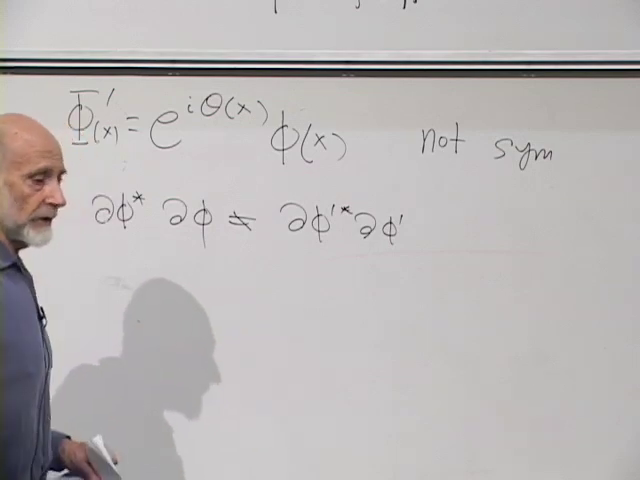
\includegraphics[width=0.78\textwidth]{lecture_08_figure_04.png}
\caption{На доске записаны локальное фазовое преобразование и то, что член с обычной производной не остается инвариантным.}
\lectureframe{00:46:49}
\label{fig:l08-local-not-symmetry}
\end{figure}

Введем векторный потенциал и последовательно зафиксируем одну конвенцию:
\begin{equation}
  D_\mu=\partial_\mu+i g A_\mu,
  \qquad
  A_\mu'=A_\mu-\frac1g\partial_\mu\theta.
  \label{eq:l08-covariant-convention}
\end{equation}
Тогда
\begin{align}
  D_\mu'\phi'
  &=
  \left(\partial_\mu+i g A_\mu'\right)
  e^{i\theta}\phi
  \notag\\
  &=
  e^{i\theta}
  \left[
    \partial_\mu\phi+i(\partial_\mu\theta)\phi
    +i g A_\mu\phi-i(\partial_\mu\theta)\phi
  \right]
  \notag\\
  &=e^{i\theta}D_\mu\phi.
  \label{eq:l08-covariant-transform}
\end{align}
Нежелательные члены сокращаются. Комплексно-сопряженная производная имеет вид
\begin{equation}
  (D_\mu\phi)^*
  =(\partial_\mu-i g A_\mu)\phi^*,
\end{equation}
и ее противоположная фаза сокращается в произведении
\begin{equation}
  (D_\mu\phi)^*D^\mu\phi.
\end{equation}

\begin{classroomqa}
\audiencequestion{Было ли преобразование калибровочного поля в предыдущей лекции записано с противоположным знаком?\lecturetimestamp{00:48:04}}
\lecturerresponse{Одновременная смена знака в \(D_\mu\) и в законе преобразования — всего лишь конвенция. При
\(D_\mu=\partial_\mu+i gA_\mu\) и
\(\phi'=e^{i\theta}\phi\) согласованность требует
\(A_\mu'=A_\mu-g^{-1}\partial_\mu\theta\). Альтернативная конвенция работает столь же хорошо, если одновременно изменить все знаки.}
\end{classroomqa}

\begin{classroomqa}
\audiencequestion{Означает ли использование на доске прописной или строчной формы \(\phi\) другое поле?\lecturetimestamp{00:55:02}}
\lecturerresponse{Никакого различия не имеется в виду. Меняющаяся форма буквы — это почерк, а не дополнительная операция и не второе скалярное поле. Существенные различия задают штрих, звездочка комплексного сопряжения и пространственно-временной индекс.}
\end{classroomqa}

\begin{classroomqa}
\audiencequestion{Является ли комплексное сопряжение той же операцией, что и поднятие или опускание лоренцева индекса в кинетическом члене?
\lecturetimestamp{00:56:50}}
\lecturerresponse{Нет. Звездочка выполняет комплексное сопряжение внутреннего комплексного поля. Лоренцевы индексы поднимаются с помощью метрики пространства-времени:
\(D^\mu=g^{\mu\nu}D_\nu\). Лоренцев скаляр требует свертки \((D_\mu\phi)^*D^\mu\phi\); обе операции здесь присутствуют и служат разным целям.}
\end{classroomqa}

\subsection{Калибровочное поле имеет собственную динамику}

Тензор напряженности поля
\begin{equation}
  F_{\mu\nu}=\partial_\mu A_\nu-\partial_\nu A_\mu
  \label{eq:l08-field-strength}
\end{equation}
калибровочно инвариантен, потому что две смешанные вторые производные от \(\theta\) сокращаются. Его компоненты время--пространство содержат электрическое поле, а компоненты пространство--пространство содержат магнитное поле. Поэтому скалярная версия электродинамики имеет вид
\begin{equation}
  \mathcal L
  =(D_\mu\phi)^*D^\mu\phi
  -V(\phi^*\phi)
  -\frac14F_{\mu\nu}F^{\mu\nu}.
  \label{eq:l08-abelian-higgs}
\end{equation}
Заряженное поле здесь бозонное. Это не электронное поле, которое является фермионным. Заряженное ядро гелия или конденсат куперовских пар показывают, как может возникнуть бозонная заряженная степень свободы.

До нарушения симметрии калибровочный член содержит производные от \(A_\mu\), но не содержит прямого массового члена. Можно было бы попытаться добавить
\begin{equation}
  \frac12m_A^2A_\mu A^\mu,
\end{equation}
но при преобразовании по уравнению~\eqref{eq:l08-covariant-convention}
\begin{equation}
  A_\mu A^\mu
  \longmapsto
  \left(A_\mu-\frac1g\partial_\mu\theta\right)
  \left(A^\mu-\frac1g\partial^\mu\theta\right),
  \label{eq:l08-bare-mass-fails}
\end{equation}
что не равно \(A_\mu A^\mu\). Затравочная масса калибровочного бозона запрещена локальной симметрией.

\begin{figure}[htbp]
\centering
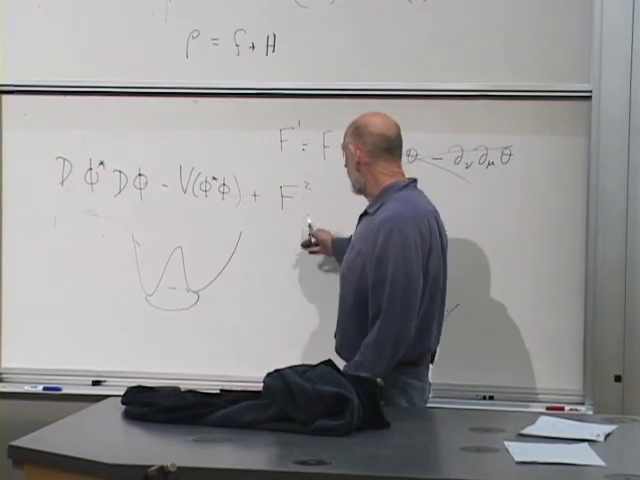
\includegraphics[width=0.76\textwidth]{lecture_08_figure_05.png}
\caption{Проверенное состояние доски для этого препятствия: при калибровочном преобразовании \(A_\mu A^\mu\) превращается в квадрат, содержащий \(\partial_\mu\theta\), так что затравочная масса векторного поля не инвариантна.}
\lectureframe{01:07:30}
\label{fig:l08-bare-mass-board}
\end{figure}

\section{Механизм Хиггса}

\subsection{Ковариантная производная порождает массу}

Вернемся к потенциалу с нарушенной симметрией и используем канонически нормированную параметризацию
\begin{equation}
  \phi(x)=\frac{f+h(x)}{\sqrt2}
  e^{i\pi(x)/f}.
\end{equation}
Ее ковариантная производная равна
\begin{equation}
  D_\mu\phi
  =
  \frac{e^{i\pi/f}}{\sqrt2}
  \left[
    \partial_\mu h
    +i(f+h)
      \left(\frac{\partial_\mu\pi}{f}+gA_\mu\right)
  \right].
  \label{eq:l08-covariant-polar}
\end{equation}
Следовательно,
\begin{equation}
\begin{aligned}
  (D_\mu\phi)^*D^\mu\phi
  ={}&
  \frac12(\partial_\mu h)^2
  \\
  &+\frac12(f+h)^2
    \left(\frac{\partial_\mu\pi}{f}+gA_\mu\right)
  \\
  &\hspace{4.2em}\times
    \left(\frac{\partial^\mu\pi}{f}+gA^\mu\right).
\end{aligned}
  \label{eq:l08-higgs-kinetic}
\end{equation}

Решающему члену не требуется никакой выбор калибровки:
\begin{equation}
  \frac12g^2f^2 A_\mu A^\mu.
  \label{eq:l08-vector-mass-term}
\end{equation}
Сравнивая его с формой Прока
\(\frac12m_A^2A_\mu A^\mu\), получаем
\begin{equation}
  \boxed{m_A=g f}.
  \label{eq:l08-vector-mass}
\end{equation}
То же разложение порождает и взаимодействия
\(g^2fh A_\mu A^\mu\) и
\(\frac12g^2h^2A_\mu A^\mu\). Следовательно, масса вектора не является произвольным нарушением калибровочной симметрии. Она возникает из калибровочно-инвариантного скалярного кинетического члена, вычисленного в фазе с ненулевой равновесной величиной \(f\).

\begin{figure}[htbp]
\centering
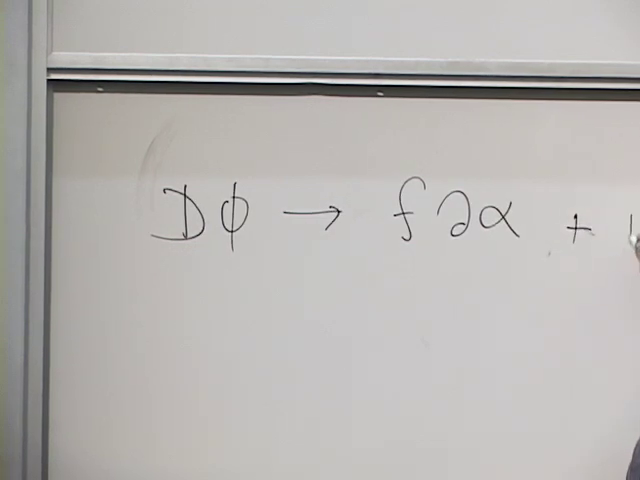
\includegraphics[width=0.78\textwidth]{lecture_08_figure_06.png}
\caption{На доске выделен вклад \(f^2A^2\) внутри \((D\phi)^*(D\phi)\). Численные множители зависят от того, как нормированы скалярное поле и калибровочная константа связи; при уравнениях~\eqref{eq:l08-canonical-polar}
и \eqref{eq:l08-covariant-convention} получается \(m_A=gf\).}
\lectureframe{01:10:10}
\label{fig:l08-generated-mass-board}
\end{figure}

В лекции \(g\) и несколько множителей \(\sqrt2\) поглощаются обозначениями на доске, поэтому при выделении массы там ненадолго чередуются \(f\), \(2f\) и \(\sqrt2f\). Эти множители не имеют инвариантного смысла, пока не заданы нормировки кинетического члена и потенциала. Устойчивый результат — \(m_A\propto gf\); уравнение~\eqref{eq:l08-vector-mass} дает множитель для используемой здесь конвенции.

\subsection{Фаза поглощается}

При калибровочном преобразовании фазовая переменная меняется как
\begin{equation}
  \pi'(x)=\pi(x)+f\,\theta(x).
\end{equation}
Выберем
\begin{equation}
  \theta(x)=-\frac{\pi(x)}{f}.
  \label{eq:l08-unitary-gauge-choice}
\end{equation}
Тогда \(\pi'=0\). Это унитарная калибровка, в которой
\begin{equation}
  \phi'(x)=\frac{f+h(x)}{\sqrt2}
\end{equation}
вещественно, и уравнение~\eqref{eq:l08-higgs-kinetic} сводится к
\begin{equation}
  (D_\mu\phi')^*D^\mu\phi'
  =
  \frac12(\partial_\mu h)^2
  +\frac12g^2(f+h)^2A_\mu'A^{\prime\mu}.
  \label{eq:l08-unitary-gauge-lagrangian}
\end{equation}
Угловое голдстоуновское поле исчезло из списка независимых переменных, а масса вектора сохраняется.

Сначала лекция показывает это в низкоэнергетическом пределе \(\rho=f\), где
\begin{align}
  \phi&=f e^{i\alpha},
  \notag\\
  D_\mu\phi
  &=if e^{i\alpha}
    \left(\partial_\mu\alpha+gA_\mu\right),
  \notag\\
  (D_\mu\phi)^*
  &=-if e^{-i\alpha}
    \left(\partial_\mu\alpha+gA_\mu\right).
  \label{eq:l08-frozen-radius}
\end{align}
Их произведение равно
\begin{equation}
  f^2
  \left(\partial_\mu\alpha+gA_\mu\right)
  \left(\partial^\mu\alpha+gA^\mu\right).
\end{equation}
Выбор \(\theta=-\alpha\) оставляет \(g^2f^2A_\mu'A^{\prime\mu}\).

\begin{figure}[htbp]
\centering
\includegraphics[width=0.82\textwidth]{lecture_08_figure_07.png}
\caption{Полная запись на доске для случая замороженного радиуса: ковариантные производные содержат вместе производную фазы и векторный потенциал. Затем в лекции выбирается \(\theta=-\alpha\), что устраняет фазу и оставляет массовый член векторного поля.}
\lectureframe{01:16:20}
\label{fig:l08-frozen-radius-board}
\end{figure}

\begin{classroomqa}
\audiencequestion{Можно ли переписать весь лагранжиан в переменных, которые явно показывают исчезновение угловой моды?
\lecturetimestamp{01:13:49}}
\lecturerresponse{Да. В полярных переменных фаза появляется только через калибровочно-инвариантную комбинацию \(\partial_\mu\alpha+gA_\mu\). Калибровочное преобразование с \(\theta=-\alpha\) обращает фазу в нуль всюду, где такая калибровка корректно определена. Кинетический член скалярного поля при этом превращается в массовый член вектора, тогда как калибровочно-инвариантный член с напряжённостью поля остаётся неизменным.}
\end{classroomqa}

\begin{classroomqa}
\audiencequestion{Неразличимы ли колебания \(\alpha\) и калибровочные колебания?\lecturetimestamp{01:18:02}}
\lecturerresponse{В калиброванной теории чистое изменение \(\alpha\), которое компенсируется соответствующим изменением \(A_\mu\), является калибровочным переописанием, а не отдельной физической волной. Инвариантная величина — \(\partial_\mu\alpha+gA_\mu\). Физическая мода, которая в глобальном случае описывалась полем Голдстоуна, вновь появляется как продольная поляризация массивного вектора.}
\end{classroomqa}

Обычно говорят, что локальная калибровочная симметрия спонтанно нарушена.
Практически такая формулировка полезна: после выбора калибровки скалярное
поле имеет ненулевое вакуумное значение, а спектр содержит массивный вектор.
Однако строго говоря, калибровочные преобразования связывают избыточные описания, а не различные физические состояния.
\editorialnote{Локальная калибровочная избыточность не нарушается в том же калибровочно-инвариантном смысле, что и глобальная симметрия. Точное утверждение состоит в том, что теория находится в фазе Хиггса. Теория возмущений с фиксированной калибровкой описывает эту фазу через ненулевое среднее значение скалярного поля и возникающий при этом спектр массивного вектора.}

\section{Куда делась голдстоуновская степень свободы}

Ничто физическое не может исчезнуть только потому, что мы сменили переменные. Подсчитайте степени свободы до и после перехода в фазу Хиггса.

До перехода:
\begin{equation}
  \underbrace{2}_{\text{massless vector}}
  +
  \underbrace{2}_{\text{complex scalar}}
  =4.
\end{equation}
У безмассового вектора две поперечные поляризации. У комплексного скаляра две действительные компоненты: радиальная и угловая.

После перехода:
\begin{equation}
  \underbrace{3}_{\text{massive vector}}
  +
  \underbrace{1}_{\text{radial Higgs}}
  =4.
  \label{eq:l08-degree-count}
\end{equation}
Массивный вектор можно перевести в состояние покоя. В его системе покоя никакое пространственное направление не является выделенным, поэтому у него должны быть три состояния поляризации. Когда он движется, две поляризации поперечные, а одна продольная. Голдстоуновская мода стала этой продольной поляризацией.

\begin{figure}[htbp]
\centering
\begin{adjustbox}{max width=\linewidth}
\begin{tikzpicture}[x=1cm,y=1cm]
  \node[draw,rounded corners,fill=blue!7,minimum width=4.3cm,
        minimum height=2.1cm,align=center] (before) at (0,0)
    {massless \(A_\mu\): \(2\) transverse\\
     \(+\)\\
     complex \(\phi\): \(h+\pi\)};
  \node[draw,rounded corners,fill=orange!10,minimum width=4.3cm,
        minimum height=2.1cm,align=center] (after) at (7,0)
    {massive \(A_\mu\): \(2\) transverse\\
     \(+\;1\) longitudinal\\
     \(+\) radial \(h\)};
  \draw[->,very thick] (before) -- node[above]{Higgs phase} (after);
  \draw[->,teal!70!black,thick]
    (-0.15,-0.65) to[bend right=28]
    node[below,align=center]{Goldstone \(\pi\) supplies\\longitudinal mode}
    (6.8,-0.65);
\end{tikzpicture}
\end{adjustbox}
\caption{Механизм Хиггса не уничтожает физические степени свободы, а перераспределяет их.}
\label{fig:l08-degree-rearrangement}
\end{figure}

\begin{classroomqa}
\audiencequestion{Как может угловая степень свободы исчезнуть, не нарушая подсчёта степеней свободы?\lecturetimestamp{01:19:13}}
\lecturerresponse{Физически она не исчезает. Безмассовый вектор имеет две спиральности, потому что его нельзя перевести в состояние покоя. Массивный вектор имеет три поляризации, включая продольную. Голдстоуновская мода становится этой третьей поляризацией, так что общий счёт остаётся прежним.}
\end{classroomqa}

В лекции предлагается полезный кинематический тест. Представьте массивную векторную частицу, замедлите её до состояния покоя, а затем разгоните в новом направлении. Поляризация, которая была поперечной относительно исходного движения, может стать продольной относительно нового движения. Точно так же, если циркулярно поляризованную массивную частицу провести через состояние покоя и направить в противоположную сторону, её метка спиральности меняется на противоположную. Строго безмассовую частицу нельзя провести через такой эксперимент, потому что ни одна инерциальная система отсчёта не может привести её к покою. Поэтому две её спиральности образуют непротиворечивый физический спектр.

\section{Сверхпроводящий аналог}

В обычном сверхпроводнике электроны образуют куперовские пары. Пара — это бозон с электрическим зарядом \(2e\), а конденсат описывается заряженным комплексным параметром порядка. Когда его модуль отличен от нуля, сочетание его фазы с электромагнитным векторным потенциалом порождает механизм Андерсона--Хиггса. Статические магнитные поля затухают на лондоновской глубине проникновения, а не распространяются свободно в толще материала. В этом точном, зависящем от среды смысле фотон ведёт себя так, как если бы он приобрёл массу.

Этот пример также проясняет различие, с которого мы начали. Электромагнитное поле не превращается навсегда в другую элементарную частицу. Характер распространения, соответствующий массивной частице, свойствен коллективному состоянию внутри материала; снаружи вакуумный фотон остаётся безмассовым.

\section{Что было установлено}

Теперь этот аргумент можно сжато изложить, не теряя его логики:
\begin{enumerate}
  \item Нарушенная глобальная непрерывная симметрия имеет плоское угловое направление и потому безмассовую голдстоуновскую моду.
  \item Локальная фазовая инвариантность требует калибровочного потенциала и заменяет \(\partial_\mu\) на \(D_\mu\).
  \item Голый массовый член \(A_\mu A^\mu\) нарушает закон локального преобразования.
  \item Когда заряженный скаляр имеет ненулевой равновесный модуль \(f\), калибровочно-инвариантный член \(|D_\mu\phi|^2\) содержит \(\frac12g^2f^2A_\mu A^\mu\).
  \item Фазу можно устранить выбором калибровки, и её физическая степень свободы становится продольной поляризацией массивного вектора.
  \item Радиальное возбуждение Хиггса остаётся, а его масса определяется кривизной скалярного потенциала.
\end{enumerate}

Следующая задача — дать массы фермионам. Электроны и кварки не могут напрямую использовать векторный механизм; их связи с Хиггсом являются взаимодействиями Юкавы. Когда скалярное поле устанавливается на \(f\), эти взаимодействия становятся массовыми членами фермионов.

Широкое утверждение о том, что без нарушения электрослабой симметрии привычные частицы были бы безмассовыми, требует ещё одного последнего уточнения. Массы элементарных кварков и заряженных лептонов, а также массы \(W\) и \(Z\), действительно обращаются в нуль вместе со средним значением поля Хиггса. Однако большая часть массы протона и нейтрона возникает динамически из конфайнмента КХД и энергии сильного поля, а не из хиггсовских масс кварков. Это различие не меняет выведенный здесь механизм Хиггса; оно лишь точно очерчивает область его применимости.
\chapter{Массы фермионов: хиральность, юкавские взаимодействия и нейтрино Майораны}

\lectureoverview{Сначала мы заново строим хиггсовский механизм для калибровочных бозонов в игрушечной \(U(1)\)-теории, а затем задаём параллельный вопрос о фермионах. Дираковский массовый член смешивает поля левой и правой хиральности, однако слабое взаимодействие приписывает им разные заряды и потому запрещает голый массовый член. Юкавское взаимодействие с полем Хиггса сохраняет симметрию; после того как поле Хиггса приобретает вакуумное значение, то же взаимодействие превращается в массу фермиона и в измеримое взаимодействие Хиггса--фермиона. В заключительной части эта логика переносится на массу нейтрино, возможные тяжёлые незащищённые частицы, кинематику космических лучей, релятивистскую инерцию и гравитацию.}

Цель вступительного повторения состоит не просто в том, чтобы повторить предыдущую лекцию. Нам нужна одна идея из неё в виде, который можно перенести на фермионы: масса — это ненулевая энергия возбуждения при нулевом импульсе. Для поля нулевой импульс означает бесконечную длину волны, или смещение, одинаковое всюду. Теория, содержащая только производные, не может обнаружить однородное смещение. Член без производных может.

\section{История калибровочных бозонов за один проход}

\subsection{Энергия, связанная с производными, и безмассовый вектор}

Модельное калибровочное поле — \(A_\mu\), а его тензор напряжённости равен
\begin{equation}
  F_{\mu\nu}
  =\partial_\mu A_\nu-\partial_\nu A_\mu .
  \label{eq:l09-field-strength}
\end{equation}
На доске кинетический член калибровочного поля схематически записан как \(F^2\). При стандартной нормировке он имеет вид
\begin{equation}
  \mathcal L_{\mathrm{gauge}}
  =-\frac14 F_{\mu\nu}F^{\mu\nu}.
  \label{eq:l09-gauge-kinetic}
\end{equation}

\begin{figure}[htbp]
\centering
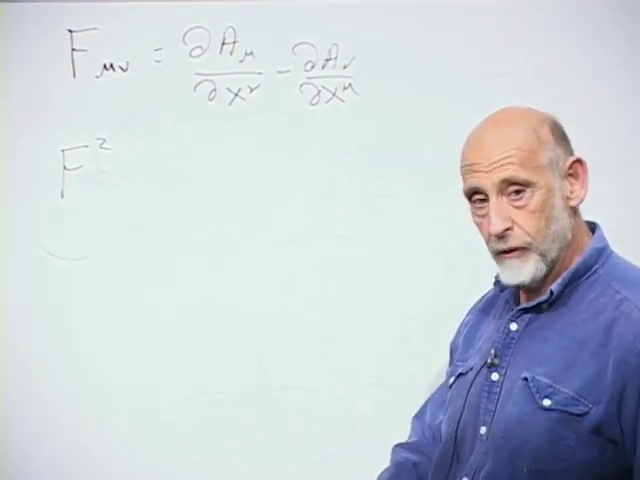
\includegraphics[width=0.72\textwidth]{lecture_09_figure_02.png}
\caption{Определение тензора напряжённости поля и используемое на доске сокращение \(F^2\) для энергии калибровочного поля, зависящей от производных.}
\lectureframe{00:02:39}
\label{fig:l09-field-strength-board}
\end{figure}

Каждое вхождение \(A_\mu\) в \eqref{eq:l09-gauge-kinetic} стоит под знаком производной. Следовательно,
\begin{equation}
  A_\mu(x)\longmapsto A_\mu(x)+c_\mu,
  \qquad \partial_\nu c_\mu=0,
\end{equation}
не изменяет \(F_{\mu\nu}\). Поэтому однородный векторный потенциал не требует энергии напряжённости поля. В терминах лекции мода с нулевым импульсом не имеет щели, и калибровочный бозон безмассов.

Это поле \(U(1)\) — намеренно простой заменитель. Физическая цель здесь — \(W^\pm\) и \(Z\), а не фотон электромагнитного взаимодействия. Ненарушенная электромагнитная симметрия оставляет фотон безмассовым; нарушенная электрослабая симметрия придаёт массы слабым калибровочным бозонам.

\subsection{Замораживание радиуса поля Хиггса}

Введём заряженное комплексное скалярное поле и запишем его в полярной форме:
\begin{equation}
  \phi(x)=\rho(x)e^{i\alpha(x)}.
\end{equation}
Его потенциал типа мексиканской шляпы минимален на окружности ненулевого радиуса. Обозначив этот радиус через \(f\), заметим, что радиальное направление сравнительно жёсткое. В первом рассмотрении мы заморозим его и оставим только фазу:
\begin{equation}
  \phi(x)\simeq f e^{i\alpha(x)}.
  \label{eq:l09-frozen-higgs}
\end{equation}

\begin{figure}[htbp]
\centering
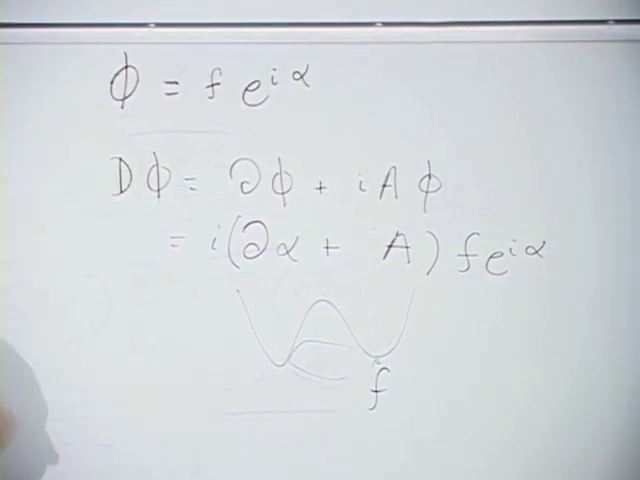
\includegraphics[width=0.72\textwidth]{lecture_09_figure_03.png}
\caption{Замороженный радиус поля Хиггса, его ковариантная производная и маленький эскиз нарушенного потенциала, использованный в повторении.}
\lectureframe{00:06:42}
\label{fig:l09-frozen-board}
\end{figure}

Выберем соглашение
\begin{equation}
\begin{aligned}
  D_\mu&=\partial_\mu+igA_\mu,
  \\
  \phi&\longmapsto e^{i\theta}\phi,
  \\
  A_\mu&\longmapsto A_\mu-\frac1g\partial_\mu\theta .
\end{aligned}
  \label{eq:l09-gauge-convention}
\end{equation}
В лекции \(g\) опускается; если оставить его явно, размерности и итоговая масса становятся ясными. Действуя на замороженное поле, получаем
\begin{align}
  D_\mu\phi
  &=(\partial_\mu+igA_\mu)f e^{i\alpha}
  \notag\\
  &=i\bigl(\partial_\mu\alpha+gA_\mu\bigr)
    f e^{i\alpha}.
  \label{eq:l09-covariant-frozen}
\end{align}
Умножение на комплексно-сопряжённое убирает фазу и одновременно превращает \(i\), умноженное на \(-i\), в \(+1\):
\begin{equation}
  |D_\mu\phi|^2
  =f^2
   \bigl(\partial_\mu\alpha+gA_\mu\bigr)
   \bigl(\partial^\mu\alpha+gA^\mu\bigr).
  \label{eq:l09-frozen-square}
\end{equation}

\begin{classroomqa}
\audiencequestion{Должен ли квадрат ковариантной производной содержать минус, потому что производная дала множитель \(i\)?
\lecturetimestamp{00:07:39}}
\lecturerresponse{Нет. Кинетический член — это произведение с комплексно-сопряжённым. Один множитель даёт \(i\), другой \(-i\), и \(i(-i)=1\). Соглашение о знаке в \(D_\mu\) можно последовательно обратить, но квадрат модуля в соответствующем выражении для энергии остаётся положительным.}
\end{classroomqa}

Комбинация в \eqref{eq:l09-frozen-square} сама является сдвинутым калибровочным полем. Выберем \(\theta=-\alpha\), чтобы фаза скаляра исчезла, и определим
\begin{equation}
  A'_\mu=A_\mu+\frac1g\partial_\mu\alpha .
  \label{eq:l09-unitary-gauge-field}
\end{equation}
Тогда
\begin{equation}
  |D_\mu\phi|^2=g^2f^2 A'_\mu A'^\mu .
  \label{eq:l09-vector-mass-term}
\end{equation}
Новый член не содержит производной от \(A'_\mu\). Однородное поле теперь запасает энергию, так что векторная мода при нулевом импульсе имеет щель.

\begin{figure}[htbp]
\centering
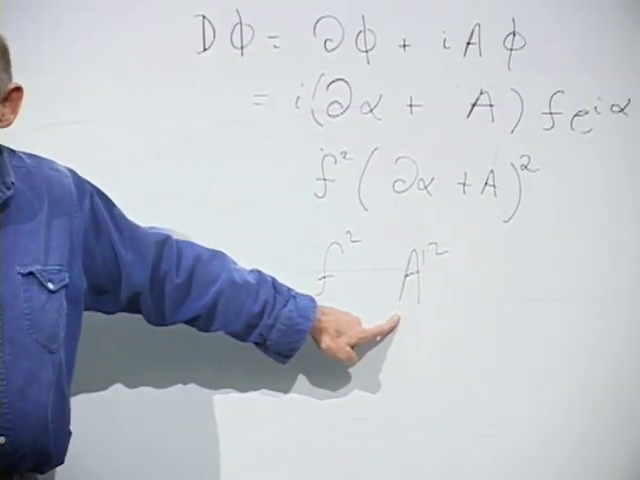
\includegraphics[width=0.72\textwidth]{lecture_09_figure_04.png}
\caption{На доске выделен член \(f^2A^2\), указывающий на массу калибровочного бозона после поглощения фазы.}
\lectureframe{00:10:31}
\label{fig:l09-vector-mass-board}
\end{figure}

При канонической нормировке скаляра пишут
\(\phi=(f+h)e^{i\pi/f}/\sqrt2\). Сравнение возникающего векторного члена с
\(\tfrac12m_A^2A_\mu A^\mu\) даёт
\begin{equation}
  m_A=gf
  \label{eq:l09-abelian-vector-mass}
\end{equation}
в этой абелевой модели. В лекции множители нормировки опускаются, и результат суммируется утверждением, что масса векторного бозона задаётся величиной \(f\).

Фазовая мода не исчезла бесследно. До введения калибровочного поля она была безмассовым бозоном Голдстоуна. После калибровки она обеспечивает продольную поляризацию, необходимую массивной векторной частице. Радиальное возбуждение, которое мы временно заморозили, остаётся физическим хиггсовским возбуждением.

\subsection{Почему член без производных означает массу}

\begin{classroomqa}
\audiencequestion{Почему член \(A'^2\) считается массовым членом, а не просто ещё одним взаимодействием?\lecturetimestamp{00:13:10}}
\lecturerresponse{Масса — это энергия в покое. Для поля частица в покое есть квант моды с нулевым импульсом и бесконечной длиной волны. Член с производными не даёт энергии статическому однородному смещению, тогда как \(m_A^2A'^2\) даёт. Эта ненулевая энергия при нулевом импульсе и есть щель по энергии покоя.}
\end{classroomqa}

Лекция развивает это утверждение через три механические аналогии.

\begin{itemize}
  \item В кристалле медленно меняющееся смещение требует упругой энергии, потому что соседние атомы смещаются по-разному. Жёсткий перенос сдвигает все атомы вместе и не требует внутренней энергии. Поэтому акустический фонон не имеет щели.
  \item В идеальном магните с вращательной симметрией пространственно меняющееся направление спина требует обменной энергии, но совместный поворот всех спинов — нет. Поэтому соответствующая длинноволновая спиновая волна не имеет щели.
  \item В плазме смещение электронной жидкости относительно положительного фона создаёт разделение зарядов и восстанавливающее электрическое поле даже при однородном относительном смещении. Поэтому плазмон имеет ненулевую частоту при нулевом волновом числе.
\end{itemize}

Калибровочное поле после механизма Хиггса ведёт себя как в третьем примере: среда с нарушенной симметрией сопротивляется тому, что иначе было бы однородным смещением без энергетической цены.

\begin{classroomqa}
\audiencequestion{До введения калибровочного поля разве фаза \(\alpha\) уже не колебалась?\lecturetimestamp{00:18:24}}
\lecturerresponse{Колебалась. Её энергия была пропорциональна \(f^2(\partial_\mu\alpha)^2\). Фаза, меняющаяся от точки к точке, имеет градиентную энергию и может распространяться, но однородное изменение фазы ничего не стоит. Это и есть безмассовая голдстоуновская мода.}
\end{classroomqa}

\begin{classroomqa}
\audiencequestion{Производная включает и производную по времени. Разве реальное перемещение всей решётки или изменение всего поля не несёт кинетической энергии?\lecturetimestamp{00:22:18}}
\lecturerresponse{Да. Сравнение проводится между статическими конфигурациями или между конфигурациями, подготовленными сколь угодно медленно. Решётка, движущаяся с ненулевой скоростью, имеет кинетическую энергию. Проверка на массу спрашивает, остаётся ли у конфигурации энергия, когда она покоится и пространственно однородна.}
\end{classroomqa}

\section{Экспериментальная подсказка: слабые взаимодействия различают левое и правое}

Теперь лекция переходит к электрону, мюону и кваркам. Их массы тоже возникают из поля Хиггса, но механизм выглядит иначе, потому что масса фермиона — это не квадратичный векторный член. Это связь между двумя хиральными полями.

\subsection{Нарушение чётности в бета-распаде}

Начнём с эмпирического факта: слабое взаимодействие нарушает чётность. Квантовая электродинамика и квантовая хромодинамика одинаково относятся к процессу и его зеркальному отражению. Слабое взаимодействие — нет. В бета-распаде нейтрона,
\begin{equation}
  n\longrightarrow p+e^-+\bar\nu_e,
  \label{eq:l09-beta-decay}
\end{equation}
высокоэнергетические электроны, отобранные взаимодействием заряженного тока, обладают левой спиральностью: их спин направлен противоположно импульсу. Соответствующие антинейтрино имеют противоположную спиральность.

Для ультрарелятивистской частицы определим спиральность как
\begin{equation}
  h=\frac{\bm S\cdot\bm p}{|\bm S|\,|\bm p|}.
\end{equation}
Спин, параллельный импульсу, имеет \(h=+1\); антипараллельный — \(h=-1\). Слабое взаимодействие связывается с левохиральным электронным полем и левохиральным нейтринным полем, но не с правохиральным электронным полем таким же образом.\editorialnote{Сначала в лекции используется лево- и праворукость в смысле спиральности, потому что при высоких энергиях это наглядно. Калибровочные заряды на самом деле действуют на хиральность — метку представления группы Лоренца, выделяемую \(P_L=(1-\gamma^5)/2\) и \(P_R=(1+\gamma^5)/2\). Для безмассовой частицы хиральность и спиральность у частиц совпадают; для массивной частицы — нет.}

Чтобы увидеть это препятствие, не вводя полный аппарат \(SU(2)_L\times U(1)_Y\), вообразим фиктивный мир \(U(1)\), в котором соответствующий заряд несёт только \(\psi_L\):
\begin{equation}
  \psi_L\longmapsto e^{i\theta}\psi_L,
  \qquad
  \psi_R\longmapsto\psi_R .
  \label{eq:l09-chiral-toy-charge}
\end{equation}
Это не электромагнетизм: реальные лево- и правохиральные электроны несут один и тот же электрический заряд. Это карикатура на слабое взаимодействие, в котором две хиральности находятся в разных электрослабых представлениях.

\begin{classroomqa}
\audiencequestion{Применима ли та же лево--правая асимметрия к кваркам?
\lecturetimestamp{00:31:50}}
\lecturerresponse{Да, при соответствующих слабых мультиплетах и гиперзарядах. Левохиральные кварки верхнего и нижнего типов образуют слабые дублеты, тогда как правохиральные поля являются слабыми синглетами. Поэтому их связи с полем Хиггса сталкиваются с той же структурной проблемой, что и у электрона.}
\end{classroomqa}

\section{Масса Дирака — это лево--правое смешивание}

\subsection{От четырёхкомпонентного уравнения к двум уравнениям Вейля}

Дираковская волновая функция имеет четыре компоненты. Грубо говоря, две из них описывают спин, а две различают решения с положительной и отрицательной энергией, причём последние переинтерпретируются как степени свободы античастицы. В гамильтоновой форме,
\begin{equation}
  i\frac{\partial\Psi}{\partial t}
  =\left(-i\bm\alpha\cdot\bm\nabla+m\beta\right)\Psi .
  \label{eq:l09-dirac-hamiltonian}
\end{equation}
Матрицы \(\alpha_i\) и \(\beta\) кодируют релятивистскую связь между энергией, импульсом и массой.

\begin{figure}[htbp]
\centering
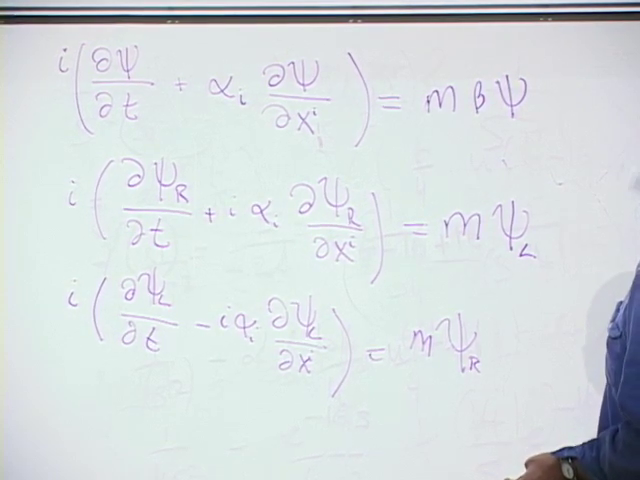
\includegraphics[width=0.74\textwidth]{lecture_09_figure_05.png}
\caption{Сначала на доске записывается уравнение Дирака, а затем оно разлагается на связанные уравнения для левохиральной и правохиральной компонент.}
\lectureframe{00:40:30}
\label{fig:l09-dirac-board}
\end{figure}

Хиральный базис делает роль \(m\) явной. При \(\sigma^\mu=(1,\bm\sigma)\) и \(\bar\sigma^\mu=(1,-\bm\sigma)\),
\begin{align}
  i\bar\sigma^\mu\partial_\mu\psi_L&=m\psi_R,
  \label{eq:l09-weyl-left}\\
  i\sigma^\mu\partial_\mu\psi_R&=m\psi_L.
  \label{eq:l09-weyl-right}
\end{align}
При \(m=0\) уравнения независимы: левохиральное поле и правохиральное поле могут распространяться, не взаимодействуя друг с другом. При \(m\neq0\) каждое из них выступает источником для другого. Именно в этом точном смысле масса Дирака смешивает левое и правое.

Сасскинд описывает это как осцилляции фермиона между левым и правым состояниями. Такая формулировка передаёт связь, но её не следует превращать в буквальную классическую картину точечной частицы, переворачивающейся туда-сюда. Точное утверждение — система связанных полевых уравнений
\eqref{eq:l09-weyl-left}--\eqref{eq:l09-weyl-right}.

\begin{classroomqa}
\audiencequestion{Согласованы ли множители \(i\) и знаки в двух уравнениях на доске?\lecturetimestamp{00:41:10}}
\lecturerresponse{Не построчно на доске; при быстром выводе один \(i\) был непоследовательно вынесен наружу. Надёжное содержание здесь — структура связи. Уравнения \eqref{eq:l09-weyl-left} и \eqref{eq:l09-weyl-right} задают одну стандартную согласованную конвенцию.}
\end{classroomqa}

\subsection{Почему слабая симметрия запрещает голую массу}

Соответствующий массовый член Дирака в лагранжиане имеет вид
\begin{equation}
  \mathcal L_m
  =-m\bar\psi\psi
  =-m\left(\bar\psi_L\psi_R+\bar\psi_R\psi_L\right).
  \label{eq:l09-bare-dirac-mass}
\end{equation}
При упрощённом преобразовании \eqref{eq:l09-chiral-toy-charge},
\begin{equation}
  \bar\psi_L\psi_R\longmapsto
  e^{-i\theta}\bar\psi_L\psi_R,
  \qquad
  \bar\psi_R\psi_L\longmapsto
  e^{i\theta}\bar\psi_R\psi_L.
\end{equation}
Ни один из этих членов не инвариантен. Поэтому до нарушения симметрии коэффициент \(m\) прямого лево--правого смешивания запрещён.

Одно лишь электромагнитное взаимодействие не создало бы этой проблемы, поскольку \(\psi_L\) и \(\psi_R\) имеют одинаковый электрический заряд. Препятствие возникает из-за их разных слабых квантовых чисел.

\subsection{Вопросы о спиральности, выявляющие тонкость хиральности}

Теперь слушатели проверяют интуитивную картину левости и правости с нескольких сторон. Эти вопросы не побочны: они точно показывают, где спиральность полезна, а где её должна заменить хиральность.

\begin{classroomqa}
\audiencequestion{Каким был бы мир, если бы слабое взаимодействие испускало электроны обеих спиральностей с равной вероятностью?\lecturetimestamp{00:42:12}}
\lecturerresponse{Непосредственная асимметрия по чётности в этом процессе исчезла бы. Но реальная электрослабая теория хиральна: в заряжённом слабом взаимодействии участвуют только левохиральные дублеты. В лекции более полный разбор того, почему природа выбрала такую структуру, откладывается.}
\end{classroomqa}

\begin{classroomqa}
\audiencequestion{Предположим, спин электрона подготовлен вертикально, а затем электрон разгоняют горизонтально. Будет ли он лево- или правоспиральным?
\lecturetimestamp{00:42:44}}
\lecturerresponse{Состояние со спином, поперечным импульсу, является суперпозицией двух спиральностей. Спиральность определена точно только тогда, когда спин параллелен или антипараллелен импульсу. Тем не менее слабые хиральные проекторы для поля определены однозначно.}
\end{classroomqa}

Массивную частицу можно замедлить до покоя и затем разогнать в противоположном направлении, не обращая её спин. Тогда её спиральность меняет знак. Безмассовую частицу нельзя ни перегнать, ни привести в состояние покоя преобразованием Лоренца, поэтому её спиральность инвариантна относительно собственных бустов. Это мотивирует сформулированное в лекции утверждение, что частица данного вида, имеющая только одну физическую спиральность, должна быть безмассовой. Более точное утверждение теории поля состоит в том, что лоренц-инвариантная масса Дирака требует обеих хиральностей.

\begin{classroomqa}
\audiencequestion{Фотон с круговой поляризацией может отразиться от зеркала и изменить направление на противоположное, ни на мгновение не переходя в состояние покоя. Не противоречит ли это аргументу о спиральности?\lecturetimestamp{00:45:28}}
\lecturerresponse{Нет. Зеркало — внешняя система, способная обмениваться угловым моментом и обращать направление распространения. Процесс отражения не является лоренцевым бустом, который перегоняет фотон. Возможность существования канала зависит также от допустимых состояний поляризации и от граничных условий на поверхности материала.}
\end{classroomqa}

\begin{classroomqa}
\audiencequestion{Содержит ли обычный электронный пучок частицы только одной спиральности или обеих?\lecturetimestamp{00:46:10}}
\lecturerresponse{Вообще говоря, обеих. Состояние массивного электрона содержит обе хиральные компоненты, а неполяризованный пучок содержит обе спиральности. Специализированные источники могут создавать поляризованный пучок с большой асимметрией по спиральности.}
\end{classroomqa}

\begin{classroomqa}
\audiencequestion{Можно ли сфокусировать пучок независимо от его спина, или магнитные поля разделяют две поляризации?\lecturetimestamp{00:46:29}}
\lecturerresponse{Обычная пространственная фокусировка может быть в значительной степени нечувствительной к спину, но магнитные моменты взаимодействуют с градиентами магнитного поля. Поэтому спин-селективные источники, градиенты типа Штерна--Герлаха и спиновая динамика в ускорителях могут подготавливать или разделять поляризации.}
\end{classroomqa}

\begin{classroomqa}
\audiencequestion{Является ли слабое различие между левым и правым всего лишь случайностью?\lecturetimestamp{00:48:13}}
\lecturerresponse{В рамках данного курса это экспериментальный факт, заложенный в Стандартную модель. Он слишком систематичен, чтобы выглядеть простым случайным совпадением, но сама Стандартная модель не выводит полный набор хиральных зарядов из более глубокого принципа.}
\end{classroomqa}

\section{Юкавская конструкция}

\subsection{Пусть Хиггс несёт недостающий заряд}

Симметрия запрещает массовый параметр в виде числа, но допускает взаимодействие с полем, которое даёт недостающую фазу преобразования. Введём комплексный скаляр с
\begin{equation}
  \phi\longmapsto e^{i\theta}\phi,
  \qquad
  \phi^\dagger\longmapsto e^{-i\theta}\phi^\dagger.
  \label{eq:l09-scalar-charge}
\end{equation}
Тогда
\begin{equation}
  \mathcal L_Y
  =-y\,\bar\psi_L\phi\psi_R
   -y^*\,\bar\psi_R\phi^\dagger\psi_L
  \label{eq:l09-yukawa-lagrangian}
\end{equation}
калибровочно инвариантно. В первом члене \(\bar\psi_L\) даёт множитель \(e^{-i\theta}\), а \(\phi\) даёт \(e^{i\theta}\); фазы сокращаются. Второй член является эрмитово-сопряжённым к первому.

Эквивалентно, хиральные уравнения приобретают зависящее от поля смешивание:
\begin{align}
  i\bar\sigma^\mu D_\mu\psi_L
    &=y\phi\psi_R,
  \label{eq:l09-yukawa-eom-left}\\
  i\sigma^\mu\partial_\mu\psi_R
    &=y^*\phi^\dagger\psi_L.
  \label{eq:l09-yukawa-eom-right}
\end{align}

\begin{figure}[htbp]
\centering
\includegraphics[width=0.76\textwidth]{lecture_09_figure_06.png}
\caption{Голая масса в правых частях заменена заряженным скалярным полем. Точные знаки на доске схематичны; инвариантная структура дана в \eqref{eq:l09-yukawa-lagrangian}.}
\lectureframe{00:51:30}
\label{fig:l09-yukawa-board}
\end{figure}

До нарушения симметрии это взаимодействие, а не масса. Правохиральный фермион может превратиться в левохиральный только при испускании или поглощении скалярного кванта, необходимого для компенсации заряда. Коэффициент \(y\) — это юкавская константа связи, а не калибровочный заряд \(g\).

\begin{classroomqa}
\audiencequestion{Допустимо ли просто поставить \(\phi\) и \(\phi^\dagger\) в правые части двух уравнений?
\lecturetimestamp{00:51:55}}
\lecturerresponse{Это допустимо именно потому, что их фазы преобразования исправляют несоответствие. Решающая проверка заключается не во внешнем виде уравнения, а в калибровочной инвариантности взаимодействия
\(\bar\psi_L\phi\psi_R+\mathrm{h.c.}\).}
\end{classroomqa}

\subsection{Вакуум превращает взаимодействие в массу}

Теперь отождествим \(\phi\) с полем Хиггса и позволим ему принять ненулевое вакуумное значение. В упрощённой нормировке лекции,
\begin{equation}
  \phi\simeq f,
\end{equation}
так что \eqref{eq:l09-yukawa-lagrangian} содержит
\begin{equation}
  \mathcal L_Y
  \supset
  -yf\,\bar\psi_L\psi_R
  -y^*f\,\bar\psi_R\psi_L .
\end{equation}
После безвредного переопределения фазы, при необходимости, масса фермиона равна
\begin{equation}
  m_f=yf.
  \label{eq:l09-lecture-fermion-mass}
\end{equation}
Это фермионный аналог векторного результата \(m_A=gf\). Тот же вакуум Хиггса, который снабжает слабые калибровочные бозоны продольной поляризацией, даёт недостающие слабые квантовые числа, необходимые для объединения левых и правых фермионов.

В канонически нормированной конвенции Стандартной модели,
\begin{equation}
  H(x)=\frac1{\sqrt2}
  \begin{pmatrix}
    0\\ v+h(x)
  \end{pmatrix},
  \qquad v\simeq246\ \mathrm{GeV},
  \label{eq:l09-sm-higgs-vacuum}
\end{equation}
и поэтому
\begin{equation}
  m_f=\frac{y_fv}{\sqrt2}.
  \label{eq:l09-sm-fermion-mass}
\end{equation}
Лекционное \(f\) и стандартное \(v/\sqrt2\) различаются только этим выбором нормировки.

\begin{classroomqa}
\audiencequestion{Если только произведение \(yf\) задаёт массу фермиона, как можно отдельно определить \(y\) и вакуумный масштаб \(f\)?\lecturetimestamp{00:55:36}}
\lecturerresponse{Массы слабых калибровочных бозонов определяют вакуумный масштаб, как только известны калибровочные константы связи. Тогда измеренная масса фермиона определяет его юкавскую константу связи. В полной теории,
\(m_W=gv/2\), \(m_Z=v\sqrt{g^2+g'^2}/2\), и
\(y_f=\sqrt2m_f/v\).}
\end{classroomqa}

\begin{classroomqa}
\audiencequestion{Масса слабого бозона составляет около \(900\ \mathrm{GeV}\)?\lecturetimestamp{00:57:43}}
\lecturerresponse{Нет; в лекции эта оговорка тут же исправляется на примерно \(90\ \mathrm{GeV}\). Точнее,
\(m_W\simeq80\ \mathrm{GeV}\) и \(m_Z\simeq91\ \mathrm{GeV}\), тогда как лежащий в основе вакуумный масштаб равен \(v\simeq246\ \mathrm{GeV}\).}
\end{classroomqa}

\subsection{Один вакуумный масштаб, много юкавских констант связи}

У каждого вида заряженного фермиона есть своя юкавская константа связи:
\begin{equation}
  m_i=y_i f
  \qquad\text{(lecture normalization)}.
  \label{eq:l09-mass-family}
\end{equation}

\begin{figure}[htbp]
\centering
\includegraphics[width=0.76\textwidth]{lecture_09_figure_08.png}
\caption{На доске зависимость от типа частицы суммирована в виде \(m_i=g_i f\); записанные там \(g_i\) — это юкавские константы связи, обозначаемые здесь как \(y_i\).}
\lectureframe{01:16:30}
\label{fig:l09-mass-family-board}
\end{figure}

Для электрона в лекции оценивается
\begin{equation}
  y_e\sim\frac{0.5\ \mathrm{MeV}}{10^2\ \mathrm{GeV}}
  \sim10^{-5}.
\end{equation}
Использование канонического значения \(v=246\ \mathrm{GeV}\) дает более точное значение
\(y_e\simeq2.9\times10^{-6}\). Топ-кварк находится на противоположном конце:
\begin{equation}
  y_t=\frac{\sqrt2m_t}{v}\simeq1.
\end{equation}
Таким образом, механизм Хиггса объясняет, как может существовать калибровочно-инвариантная масса, но
он не объясняет огромную иерархию среди \(y_i\). Наблюдаемые
массы фермионов лишь переводят эту иерархию в измеренные числа.

\begin{classroomqa}
\audiencequestion{Неужели у топ-кварка действительно юкавская константа связи порядка
единицы?\lecturetimestamp{00:59:09}}
\lecturerresponse{Да. Его масса сравнима с электрослабым масштабом, поэтому
его константа связи — не крошечное пертурбативное число, как у электрона. В
современной нормировке величина \(y_t\) близка к единице.}
\end{classroomqa}

\subsection{Восстановление физической флуктуации поля Хиггса}

Фиксация скалярного поля на его вакуумном значении скрыла радиальное возбуждение. Схематически
восстановим его:
\begin{equation}
  \phi(x)\simeq f+h(x).
\end{equation}
Юкавский множитель становится
\begin{equation}
  y\phi\simeq yf+yh=m_f+yh.
  \label{eq:l09-mass-plus-higgs}
\end{equation}

\begin{figure}[htbp]
\centering
\includegraphics[width=0.76\textwidth]{lecture_09_figure_07.png}
\caption{На доске флуктуация Хиггса восстановлена внутри юкавского члена:
постоянная часть порождает массу фермиона, а флуктуирующая часть
порождает испускание или поглощение бозона Хиггса.}
\lectureframe{01:01:15}
\label{fig:l09-higgs-fluctuation-board}
\end{figure}

Первый член в \eqref{eq:l09-mass-plus-higgs} — это масса. Второй — вершина,
в которой бозон Хиггса взаимодействует с фермионом. В канонической нотации
Стандартной модели
\begin{equation}
  \mathcal L_Y
  \supset
  -m_f\bar\psi\psi
  -\frac{m_f}{v}h\bar\psi\psi.
  \label{eq:l09-higgs-fermion-vertex}
\end{equation}
Константа связи пропорциональна массе фермиона. С учетом кинематики,
цветовых факторов, фазового объема и конкурирующих каналов Хиггс поэтому
сильнее взаимодействует с более тяжелыми фермионами.

\begin{classroomqa}
\audiencequestion{Являются ли сами константы связи вероятностями?
\lecturetimestamp{01:03:35}}
\lecturerresponse{Они входят в квантовые амплитуды. Простая скорость процесса часто
пропорциональна квадрату модуля амплитуды и, следовательно, квадрату константы
связи, но важны также фазовый объем, суммы по спинам, интерференция, петли и
несколько вершин. Константу связи не следует напрямую отождествлять с
вероятностью.}
\end{classroomqa}

\begin{classroomqa}
\audiencequestion{Предполагает ли этот аргумент, что существует только одно поле
Хиггса?\lecturetimestamp{01:03:59}}
\lecturerresponse{Здесь описывается минимальная Стандартная модель, в которой есть один
комплексный дублет Хиггса. Три из его четырех вещественных компонент поглощаются
калибровочными бозонами \(W^\pm\) и \(Z\), оставляя один физический нейтральный скаляр. Расширения могут
содержать больше дублетов или другие скалярные мультиплеты. Суперсимметричные модели
обычно требуют двух дублетов Хиггса и потому содержат несколько физических
хиггсовских состояний.}
\end{classroomqa}

Это историческое ожидание теперь можно сравнить с экспериментом.
\editorialnote{Эта лекция была записана до открытия бозона Хиггса. ATLAS и
CMS объявили о хиггсоподобной частице в 2012, теперь измеряемой вблизи
\(125\ \mathrm{GeV}\). Ее наблюдаемые константы связи в целом согласуются
с картиной Стандартной модели, в которой они пропорциональны массе. Утверждение,
что она распадается преимущественно на самые тяжелые частицы, всегда сопровождается
кинематической оговоркой: пара \(t\bar t\) на массовой оболочке слишком тяжела для бозона Хиггса с массой \(125\ \mathrm{GeV}\).
}

\section{Античастицы, пучки и смысл киральности}

Прежде чем перейти к нейтрино, на занятии возвращаются к нескольким практическим
вопросам об античастицах и пучках ускорителей.

\begin{classroomqa}
\audiencequestion{Какую ручность имеет античастица левого
электрона?\lecturetimestamp{01:06:05}}
\lecturerresponse{Левокиральное электронное поле уничтожает электроны с левой спиральностью
и создает позитроны с правой спиральностью в ультрарелятивистском
пределе. Это один из случаев, где различие между частицей и античастицей, а также между киральностью
и спиральностью, нужно формулировать особенно аккуратно.}
\end{classroomqa}

\begin{classroomqa}
\audiencequestion{Могут ли электрон и позитрон столкнуться с образованием бозона \(Z\)?\lecturetimestamp{01:07:13}}
\lecturerresponse{Да, когда их энергия в системе центра масс соответствует разрешенному
каналу. Электрон--позитронные коллайдеры с большой
точностью исследовали резонанс \(Z\). Заряд и остальные квантовые числа сохраняются во всем
процессе.}
\end{classroomqa}

\begin{classroomqa}
\audiencequestion{Все ли позитроны рождаются в одном специальном слабом
процессе?\lecturetimestamp{01:07:37}}
\lecturerresponse{Нет. Рождение пар — стандартный электромагнитный механизм.
Например, энергичный электрон может испустить виртуальный фотон, и этот
фотон может породить пару \(e^-e^+\) в поле другой частицы. В
лекции это набросано с помощью диаграммы Фейнмана.}
\end{classroomqa}

\begin{classroomqa}
\audiencequestion{Может ли линейный ускоритель выбирать скорость или энергию своих
электронов?\lecturetimestamp{01:09:24}}
\lecturerresponse{Да. Ускоряющие поля и синхронизация задают диапазон энергий.
Как только электроны становятся ультрарелятивистскими, их скорость и без того уже чрезвычайно
близка к \(c\), так что дополнительная энергия ускорителя в основном увеличивает импульс
и полную энергию, а не заметно повышает скорость.}
\end{classroomqa}

\begin{classroomqa}
\audiencequestion{Может ли ускоритель подготовить пучок одной поляризации?
\lecturetimestamp{01:09:47}}
\lecturerresponse{Да, хотя это технически сложно. Можно приготовить
спин-поляризованные электроны при низкой энергии с помощью источника, зависящего от спина, а затем
ускорить их, контролируя прецессию спина. Современные коллайдеры количественно характеризуют
получающуюся поляризацию пучка, а не считают ее идеально чистой.}
\end{classroomqa}

\section{Масса нейтрино и майорановская возможность}

\subsection{Почему масса нейтрино потребовала расширения}

Первоначальная минимальная Стандартная модель включала только левокиральные нейтринные
поля и потому предсказывала безмассовые нейтрино. Осцилляции нейтрино
показывают, что по меньшей мере два собственных значения нейтринной массы различаются и что массы нейтрино
ненулевые, хотя и малы по сравнению с массами заряженных фермионов.

\begin{classroomqa}
\audiencequestion{Насколько малы массы нейтрино и где находится их
правокиральная компонента?\lecturetimestamp{01:10:38}}
\lecturerresponse{Осцилляции определяют разности квадратов масс, а не
абсолютные массы. Соответствующие расщепления отвечают масштабам порядка
\(0.009\ \mathrm{eV}\) и \(0.05\ \mathrm{eV}\). Дираковское описание добавляет
стерильные правокиральные нейтрино; майорановское описание вместо этого связывает
недостающую киральность с зарядово-сопряженными нейтринными полями.}
\end{classroomqa}

Для дираковского нейтрино добавляют новое поле \(\nu_R\) и повторяют юкавскую
конструкцию:
\begin{equation}
  \mathcal L_{\nu,\mathrm{Dirac}}
  =-y_\nu\bar L\,\widetilde H\,\nu_R+\mathrm{h.c.},
  \qquad
  m_\nu=\frac{y_\nu v}{\sqrt2}.
  \label{eq:l09-dirac-neutrino}
\end{equation}
Требуемая величина \(y_\nu\) чрезвычайно мала.

Существует и другая логическая возможность, поскольку нейтрино не несет
электрического заряда. Левокиральное нейтрино можно связать с собственным зарядово-
сопряженным полем, которое имеет противоположную киральность:
\begin{equation}
  \nu_L\longleftrightarrow(\nu_L)^c_R .
  \label{eq:l09-majorana-mixing}
\end{equation}
Массовое собственное состояние, построенное таким образом, является майорановским фермионом:
это своя собственная античастица, с точностью до фазовых соглашений. Аналогичное электрон--позитронное
смешивание запрещено, поскольку оно нарушало бы точное сохранение
электрического заряда.

\begin{classroomqa}
\audiencequestion{Почему смешивание частица--античастица разрешено для
нейтрино, но не для электрона?\lecturetimestamp{01:13:43}}
\lecturerresponse{Электрон и позитрон имеют противоположные электрические заряды,
так что массовый член, который смешивал бы их как одно и то же одночастичное состояние, нарушал бы
ненарушенную электромагнитную симметрию. Нейтрино электрически нейтрально.
Если никакое точное сохраняющееся лептонное число не отличает его от античастицы,
майорановская масса допустима.}
\end{classroomqa}

Название дано в честь Этторе Майораны, молодого итальянского физика, который сформулировал
такой тип вещественного фермионного представления и исчез в 1938 году. В
лекции делают паузу на этой исторической загадке: его судьба так и не была установлена.
\editorialnote{До электрослабого нарушения симметрии калибровочно-инвариантная майорановская масса для активного нейтрино
Стандартной модели не является перенормируемым голым членом. При
низких энергиях она может возникать из оператора Вайнберга размерности пять
\((LH)(LH)/\Lambda\) или через механизм seesaw с участием тяжелых стерильных нейтрино.
Остается экспериментально неустановленным, являются ли нейтрино дираковскими или
майорановскими частицами.}

\section{Почему знакомый спектр группируется вблизи электрослабого масштаба}

\subsection{Общий масштаб и связанные с ним важные оговорки}

\begin{classroomqa}
\audiencequestion{Почему ожидалось, что масса Хиггса окажется в области
слабого масштаба?\lecturetimestamp{01:14:48}}
\lecturerresponse{Кривизна потенциала Хиггса задает массу
радиального возбуждения Хиггса, тогда как тот же вакуумный масштаб \(f\) задает массы \(W\) и \(Z\).
Поэтому при отсутствии экстремальной скалярной самосвязи ожидалось, что
масса Хиггса будет того же широкого порядка, что и слабый масштаб. Наблюдаемое
значение \(125\ \mathrm{GeV}\) действительно лежит там.}
\end{classroomqa}

Яркое резюме лекции состоит в том, что элементарные массы минимальной
Стандартной модели восходят к одному вакуумному состоянию с нарушенной симметрией:
\begin{align}
  m_W&=\frac12gv,\\
  m_Z&=\frac12\sqrt{g^2+g'^2}\,v,\\
  m_f&=\frac1{\sqrt2}y_fv.
  \label{eq:l09-electroweak-mass-summary}
\end{align}
Если бы \(v\) обращалось в нуль при фиксированных безразмерных константах связи,
слабые калибровочные бозоны и заряженные элементарные фермионы были бы безмассовыми.

Это утверждение не следует распространять за пределы области его применимости. Фотон и глюоны остаются безмассовыми, поскольку их защищает ненарушенная калибровочная симметрия. Большая часть массы протона и нейтрона — это энергия связи КХД, а не сумма хиггсовских масс их кварков. Масса нейтрино требует расширения минимальной модели. Сама масса бозона Хиггса зависит от скалярного потенциала и не является просто еще одной массой Юкавы.

\subsection{Частицы, масса которых не обязана ждать нарушения симметрии}

Предположим, что новый фермион имел бы лево- и право-хиральные компоненты с одинаковыми калибровочными квантовыми числами. Тогда член \(\bar\Psi_L\Psi_R+\mathrm{h.c.}\) уже был бы калибровочно-инвариантным. Такой \emph{вектороподобный} фермион мог бы иметь голую массу \(M\), не связанную с \(v\):
\begin{equation}
  \mathcal L_{\mathrm{vectorlike}}
  =-M\bar\Psi\Psi.
  \label{eq:l09-vectorlike-mass}
\end{equation}
Электрослабая симметрия не накладывает запрета на \(M\gg v\).

Это мотивирует общий аргумент лекции, связанный с естественностью. Частицы, защищенные калибровочной или хиральной симметрией, остаются безмассовыми, пока вакуум Хиггса не нарушит эту защиту, так что их массы привязаны к относительно малому масштабу \(v\). Частицы, у которых нет такой защиты, естественным образом могут быть гораздо тяжелее и потому отсутствовать в наблюдаемом низкоэнергетическом спектре. То, что мы видим, может быть результатом эффекта отбора: доступные частицы — это те, чьи массы были вынуждены ждать нарушения электрослабой симметрии.

\begin{classroomqa}
\audiencequestion{Не играли бы частицы с независимыми и гораздо большими массами никакой роли в реальности?\lecturetimestamp{01:19:39}}
\lecturerresponse{В обычной низкоэнергетической лабораторной физике они играли бы небольшую роль, потому что их трудно рождать, но они все же могли бы определять высокоэнергетическую историю или космологию. В лекции темная материя приводится как возможная область, где более тяжелый скрытый спектр мог бы впервые проявиться.}
\end{classroomqa}

Обсуждение в 2010 году отражает тогдашнее популярное ожидание темной материи на электрослабом масштабе или несколько выше. Это по-прежнему полезный класс моделей, а не установленный факт. Темная материя обнаружена гравитационно, но то, какой частицей она является, и происхождение ее массы остаются неизвестными.

\section{Заключительные вопросы: космические лучи, инерция, гравитация и хиральность}

\subsection{Масса — не то же самое, что большая лабораторная энергия}

\begin{classroomqa}
\audiencequestion{Какова масса космического луча?
\lecturetimestamp{01:20:57}}
\lecturerresponse{Космический луч может быть протоном, атомным ядром, электроном или фотоном; его инвариантная масса есть масса этой частицы или системы. Поразительна его лабораторная энергия, которая для самых высокоэнергетических событий достигает примерно от \(10^{20}\) до \(10^{21}\ \mathrm{eV}\). Большая энергия — не то же самое, что большая инвариантная масса.}
\end{classroomqa}

Космический луч сталкивается с частицей-мишенью, которая приближенно покоится. Для налетающего протона с лабораторной энергией \(E\gg m_p\),
\begin{equation}
  s=(p_1+p_2)^2
  \simeq2m_pE+2m_p^2,
  \qquad
  \sqrt{s}\simeq\sqrt{2m_pE}.
  \label{eq:l09-fixed-target-s}
\end{equation}
В энергию центра масс переходит только квадратный корень из энергии налетающей частицы. Для двух встречных пучков с одинаковой энергией \(E_{\rm beam}\),
\begin{equation}
  \sqrt{s}\simeq2E_{\rm beam}.
  \label{eq:l09-collider-s}
\end{equation}
Вот почему коллайдер гораздо эффективнее неподвижной мишени при преобразовании контролируемой энергии пучка в массу новых частиц.

\begin{classroomqa}
\audiencequestion{Почему коллайдер CERN может быть более мощным инструментом исследования, чем одна гораздо более энергичная частица, налетающая на покоящееся вещество?
\lecturetimestamp{01:21:50}}
\lecturerresponse{При столкновении с неподвижной мишенью сохранение импульса уносит большую часть лабораторной энергии вперед, в движение конечного состояния. В симметричном коллайдере полный пространственный импульс может обращаться в нуль, оставляя энергию пучков доступной как энергию центра масс. Самые высокоэнергетические космические лучи все же могут превзойти LHC по \(\sqrt{s}\), но они приходят непредсказуемо и не могут обеспечить светимость коллайдера или контролируемые условия детектора.}
\end{classroomqa}

\subsection{Масса покоя и сопротивление ускорению}

\begin{classroomqa}
\audiencequestion{Являются ли инерция и масса по существу одним и тем же?
\lecturetimestamp{01:22:41}}
\lecturerresponse{В покое инвариантная масса является и энергией покоя через \(E_0=mc^2\), и параметром, определяющим отклик на силу при малых скоростях. Специальная теория относительности объясняет, почему эти определения относятся к одной и той же величине. Для движущихся тел яснее считать инвариантную массу фиксированной и описывать ускорение через релятивистские энергию и импульс.}
\end{classroomqa}

Инвариантное соотношение
\begin{equation}
  E^2=p^2c^2+m^2c^4
  \label{eq:l09-energy-momentum}
\end{equation}
содержит оба этих смысла. Вблизи покоя,
\begin{equation}
  E=mc^2+\frac{p^2}{2m}+\cdots,
\end{equation}
так что тот же самый \(m\), который дает энергию покоя, фигурирует и в кинетическом отклике. При большой скорости связь между силой и ускорением зависит от того, параллельна ли сила скорости или перпендикулярна ей. Именно из-за этой зависимости от направления в современных изложениях избегают зависящей от скорости \emph{релятивистской массы} и оставляют слово масса для лоренц-инвариантной величины \(m\).

\subsection{С чем взаимодействует гравитация}

\begin{classroomqa}
\audiencequestion{После того как Хиггс придает частице массу, начинает ли она тогда взаимодействовать с гравитацией?\lecturetimestamp{01:23:58}}
\lecturerresponse{Ее энергия покоя вносит вклад в гравитацию, но масса — не весь источник. Фотоны безмассовы и тем не менее отклоняются гравитацией. В общей теории относительности источником служит тензор энергии--импульса: плотность энергии, поток импульса, давление и напряжение. Для медленно движущегося вещества доминирующий вклад дает его энергия покоя.}
\end{classroomqa}

Отклонение света вблизи Солнца показывает это в операциональном смысле. Фотон реагирует на кривизну пространства-времени, несмотря на \(m=0\), и его энергия и импульс тоже вносят вклад в гравитационное поле. Для двух почти статических массивных тел энергия определяется главным образом \(mc^2\), поэтому ньютоновскую гравитацию можно записывать через их массы, не выписывая более общую формулировку через тензор энергии--импульса.

\begin{classroomqa}
\audiencequestion{Труднее ли ускорять высокоэнергетическую частицу одним и тем же образом во всех направлениях?\lecturetimestamp{01:25:20}}
\lecturerresponse{Нет. Изменение импульса при силе, параллельной движению, отличается от изменения при поперечной силе. Верно, что более энергичную частицу труднее отклонить, но приписывание ей одной увеличенной массы при движении скрывает эту направленную структуру.}
\end{classroomqa}

\subsection{Электрон в покое и обещанное различие}

\begin{classroomqa}
\audiencequestion{Как можно называть покоящийся электрон левоспиральным или правоспиральным?\lecturetimestamp{01:26:32}}
\lecturerresponse{В состоянии покоя ему нельзя приписать спиральность, поскольку спиральность использует направление импульса. Однако спинор покоя все же можно разложить на лево- и право-хиральные компоненты. Для массивного электрона присутствуют обе компоненты, и массовый член связывает их.}
\end{classroomqa}

\begin{classroomqa}
\audiencequestion{Если электрон в покое не имеет спиральности, может ли он все же участвовать в слабом взаимодействии?\lecturetimestamp{01:27:18}}
\lecturerresponse{Да. Слабое взаимодействие сопрягается с хиральностью, а не с зависящей от системы отсчета меткой спиральности. При высокой энергии спиральность служит удобным приближением к хиральности; вблизи покоя это упрощение не работает. Именно это тонкое различие лекция и отложила.}
\end{classroomqa}

\section{Исторические вопросы в конце лекции}

\subsection{Предоткрытийное окно Хиггса}

В 2010 году бозон Хиггса еще не был обнаружен. Прецизионные электрослабые наблюдаемые, особенно чувствительные к петлевым поправкам соотношения между \(W\), \(Z\), топ-кварком и другими параметрами, указывали в рамках Стандартной модели на сравнительно легкий бозон Хиггса. В лекции приводится вероятная верхняя область вблизи \(160\ \mathrm{GeV}\), значительно ниже \(v\), но не отделенная от него порядком величины.

\begin{classroomqa}
\audiencequestion{Какие свидетельства тогда указывали на то, что бозон Хиггса легче вакуумного масштаба \(250\ \mathrm{GeV}\)?\lecturetimestamp{01:28:28}}
\lecturerresponse{Высокоточные измерения можно было сравнивать с радиационными поправками, значения которых логарифмически зависят от массы бозона Хиггса. Получающиеся глобальные подгонки благоприятствовали легкому бозону Хиггса. Это было косвенное свидетельство, а не прямое измерение массы; более позднее прямое значение составляет около \(125\ \mathrm{GeV}\).}
\end{classroomqa}

\begin{classroomqa}
\audiencequestion{Могли бы несколько минимумов потенциала Хиггса давать разные значения \(f\), возможно связанные с разными поколениями частиц?
\lecturetimestamp{01:29:28}}
\lecturerresponse{Разные минимумы могут соответствовать очень разной низкоэнергетической физике, но из наблюдаемых поколений нельзя просто заключить о наличии нескольких минимумов потенциала Хиггса. Лекция откладывает более широкую тему множественных вакуумов до более позднего курса, а не делает вид, будто здесь она уже решена.}
\end{classroomqa}

\begin{classroomqa}
\audiencequestion{Ожидалось ли, что бозон Хиггса станет первой новой частицей, обнаруженной на LHC?\lecturetimestamp{01:31:32}}
\lecturerresponse{Не обязательно. Его наблюдаемость зависит от скоростей рождения и каналов распада, некоторые из которых могут быть трудными для наблюдения или невидимыми. До появления данных LHC можно было правдоподобно ожидать, что первыми проявятся суперсимметричные или другие новые частицы. Исторически бозон Хиггса был открыт, а ни одна суперсимметричная частица пока не была надежно установлена.}
\end{classroomqa}

\subsection{Когда нейтральная частица является собственной античастицей}

\begin{classroomqa}
\audiencequestion{У фотона и глюона нет античастиц потому, что они безмассовы?\lecturetimestamp{01:32:12}}
\lecturerresponse{Нет. Безмассовость не является критерием. Фотон является собственной античастицей, потому что не существует сохраняющегося заряда, который отличал бы фотон от антифотона. Каждый глюон также является самосопряжённым калибровочным квантом в соответствующем цветовом представлении, хотя сами глюоны несут цвет, и цветовые метки перемешиваются при зарядовом сопряжении. Нейтрон электрически нейтрален, но имеет отличимый антинейтрон, поскольку барионное число и кварковый состав различают их.}
\end{classroomqa}

Нейтрино снова оказывается тонким случаем. Оно участвует в слабых взаимодействиях, и ультрарелятивистские состояния, называемые нейтрино и антинейтрино, взаимодействуют с противоположными спиральностями. Если их различает точно сохраняющееся лептонное число, они могут образовывать частицу Дирака с отличной от неё античастицей. Если лептонное число не является точным, а масса — майорановская, то массивная частица является собственной античастицей, хотя два её состояния спиральности ведут себя по-разному в слабых процессах.

\begin{classroomqa}
\audiencequestion{Доказывают ли слабый заряд и лептонное число, что нейтрино и антинейтрино обязательно различны?\lecturetimestamp{01:32:46}}
\lecturerresponse{Не решающим образом. Слабые взаимодействия различают состояния спиральности, но майорановская масса может объединять поле нейтрино с его зарядово-сопряжённым полем. Решающим является вопрос о том, запрещает ли это смешивание какое-либо точно сохраняющееся квантовое число. Полное лептонное число не предписывается Стандартной моделью как точная калибровочная симметрия.}
\end{classroomqa}

Обычные осцилляции ароматов требуют отдельной оговорки.
\editorialnote{Обычные наблюдаемые осцилляции ароматов смешивают
\(\nu_e,\nu_\mu,\nu_\tau\) в пределах одного и того же сектора нейтрино или антинейтрино; сами по себе они не демонстрируют превращения нейтрино--антинейтрино.
Процессы с нарушением лептонного числа, такие как безнейтринный двойной бета-распад, дали бы прямое свидетельство майорановской массы, но пока ни один из них не подтверждён.}

\begin{classroomqa}
\audiencequestion{Объясняет ли Стандартная модель, почему электрические заряды квантуются?\lecturetimestamp{01:33:39}}
\lecturerresponse{В лекции этот вопрос отмечается, но не разбирается. В рамках Стандартной модели калибровочная инвариантность и компенсация аномалий сильно ограничивают допустимые присвоения гиперзаряда; более глубокое объяснение часто апеллирует к великому объединению или иной ультрафиолетовой структуре.}
\end{classroomqa}

\section{Что было установлено в лекции}

Теперь объяснения для калибровочных бозонов и фермионов согласуются.

\begin{enumerate}
  \item Калибровочная теория с одними лишь производными не имеет энергетической щели для однородного векторного потенциала. Калибровочная симметрия запрещает голую массу векторного поля.
  \item Заряженный скаляр с ненулевым вакуумным модулем вносит вклад \(g^2f^2A_\mu A^\mu\). Его угловая голдстоуновская мода становится продольной поляризацией массивного слабого калибровочного бозона.
  \item Дираковская масса связывает \(\psi_L\) и \(\psi_R\). Поскольку слабое взаимодействие приписывает им разные калибровочные квантовые числа, голый лево--правый массовый член запрещён.
  \item Взаимодействие Юкавы помещает поле Хиггса между двумя хиральностями и является калибровочно-инвариантным. Замена поля Хиггса его вакуумным значением даёт \(m_f=y_ff\), тогда как сохранение его флуктуации даёт физическое взаимодействие Хиггс--фермион.
  \item Масса нейтрино подчиняется той же лево--правой логике, но допускает как дираковскую, так и майорановскую реализации, поскольку нейтрино электрически нейтрально.
  \item Частицы без калибровочной или хиральной защиты могли бы иметь массы, не связанные с электрослабым масштабом, и могут находиться далеко за пределами досягаемости нынешних экспериментов.
\end{enumerate}

Объединяющее утверждение, следовательно, не состоит в том, что Хиггс — это вещество, которое механически тормозит частицы. Оно состоит в том, что электрослабый вакуум имеет ненулевой скалярный параметр порядка. Этот параметр порядка изменяет, какие калибровочно-инвариантные члены возможны в низкоэнергетических уравнениях. Для векторов он создаёт щель при нулевом импульсе; для фермионов допускает лево--правое смешивание. Тогда разные массы измеряют разные константы связи с одним и тем же вакуумом с нарушенной симметрией.
\chapter{Масштаб Хиггса, бегущие константы связи и проблема иерархии}

\lectureoverview{Заключительная лекция начинается с взгляда за пределы Стандартной модели — в сторону объединения, суперсимметрии и проблемы калибровочной иерархии. Чтобы понять, почему поле Хиггса находится в центре этих вопросов, мы сначала восстанавливаем лагранжиан Дирака и показываем, что масса фермиона смешивает левую и правую киральности. Киральное слабое взаимодействие запрещает такую массу как голый член; калибровочно-инвариантная связь Юкавы даёт её только после того, как поле Хиггса приобретает вакуумное значение. Затем мы выводим это вакуумное значение из потенциала Хиггса, спрашиваем, почему каждая известная элементарная масса привязана к этому одному малому масштабу, и используем сверхпроводимость как физическую аналогию. После перерыва лекция выводит ренормализацию из экранирования в проводнике и диэлектрике, переносит рассуждение на QED и QCD, прослеживает калибровочные константы связи в направлении объединения и выводит планковский масштаб из гравитации на малых расстояниях. Затем электрослабый масштаб возвращается как единственное необъяснённое малое число.}

\section{Вопрос, который ждёт нас за пределами Стандартной модели}

Стандартная модель представляется здесь не как замкнутый каталог. В начале сегодняшней лекции я хочу сказать, куда пойдёт следующий курс. У этой теории есть трудности, а не логические парадоксы: проблема калибровочной иерархии, возможная роль суперсимметрии и вопрос об объединении. Три калибровочных множителя
\begin{equation}
  SU(3)_c\times SU(2)_L\times U(1)_Y
  \label{eq:l10-standard-model-group}
\end{equation}
по отдельности описывают сильное, слабое и гиперзарядовое взаимодействия. Могут ли они быть подгруппами одной большей группы? Часто изучаемая возможность — \(SU(5)\), где кварки и лептоны входят в общие мультиплеты. Пользуется ли природа именно этой конструкцией — другой вопрос. Важная подсказка состоит в том, что кажущиеся раздельными структуры удивительно аккуратно укладываются в более крупную математическую структуру.

Большой адронный коллайдер был построен отчасти для того, чтобы выявить физику, которая разрешает эти вопросы. В 2010 его ближайшей целью был бозон Хиггса. Обнаружение Хиггса никак не могло означать просто добавление одной частицы в таблицу. Хиггс опознаётся по взаимосвязанному набору свойств: его вакуумное значение сообщает массы слабым векторным бозонам и фермионам, тогда как его флуктуация взаимодействует с теми же частицами с определёнными силами связи. Резонанс с неправильными связями не был бы хиггсовским бозоном Стандартной модели. \editorialnote{Лекция предшествует открытию 2012 года. Наблюдаемый скаляр с массой приблизительно \(125\,\mathrm{GeV}\) имеет, в пределах нынешней точности, спин, чётность и картину связей, ожидаемые для хиггсовского бозона Стандартной модели. По состоянию на 2026 низкоэнергетических суперсимметричных частиц не наблюдалось. Эти более поздние факты уточняют исторический контекст, не меняя рассуждения, развиваемого в аудитории.}

Путь к этому рассуждению начинается не с потенциала Хиггса, а с уравнения Дирака. Прежде чем спрашивать, откуда берётся масса фермиона, нужно точно понять, что именно она делает.

\section{От уравнения Дирака к его лагранжиану}

\subsection{Старая нотация Дирака}

В гамильтоновой нотации, использовавшейся, когда уравнение Дирака было впервые введено, его структура такова:
\begin{equation}
  i\partial_t\psi
  =
  \left(-i\alpha^i\partial_i+\beta m\right)\psi .
  \label{eq:l10-dirac-hamiltonian}
\end{equation}
Знаки и множители при \(i\) зависят от соглашений, и на доске некоторые из них временно опущены. Инвариантное содержание состоит в разделении между членами, содержащими производные, и массовым членом, не содержащим их.

\begin{figure}[htbp]
\centering
\includegraphics[width=0.82\textwidth]{lecture_10_figure_02.png}
\caption{Уравнение Дирака и лагранжиан в старой нотации \(\alpha,\beta\). Доска используется здесь для показа структуры, а не как фиксированное соглашение о знаках.}
\lectureframe{00:05:52}
\label{fig:l10-dirac-alpha-beta}
\end{figure}

Чтобы получить действие, вариация которого даёт уравнение Дирака, умножим это уравнение на \(\psi^\dagger\). Перенос всех членов в одну сторону устраняет нужду в знаке равенства, что и порождает небольшую математическую шутку этой лекции: как только уравнение записано как выражение, обращающееся в нуль, знак равенства уже сделал своё дело. Соответствующий лагранжиан первого порядка можно схематически записать как
\begin{equation}
  \mathcal L
  =
  \psi^\dagger
  \left(i\partial_t+i\alpha^i\partial_i-\beta m\right)\psi ,
  \label{eq:l10-dirac-old-lagrangian}
\end{equation}
при понимании, что согласованное метрическое соглашение фиксирует относительные знаки.

Члены с производными переносят возбуждение из одной точки пространства-времени в соседнюю и при этом вращают его спинорные компоненты. В решёточной картине это члены перескока. Напротив, массовый член поглощает и вновь испускает фермион в той же самой точке. Производной в нём нет. Вскоре окажется, что эта локальная операция представляет собой повторяющееся превращение между двумя киральностями.

\begin{classroomqa}
\audiencequestion{Нужно ли ставить \(\gamma^0\) после \(\psi^\dagger\)?\lecturetimestamp{00:05:59}}
\lecturerresponse{Не в той нековариантной форме, которая только что была записана. Но вопрос прямо подводит к ковариантной нотации. Определим дираково сопряжение как \(\bar\psi=\psi^\dagger\gamma^0\); тогда \(\gamma^0\) действительно уже входит в объект, стоящий слева.}
\end{classroomqa}

\subsection{Ковариантная форма}

Введём
\begin{equation}
  \bar\psi\equiv\psi^\dagger\beta
  =\psi^\dagger\gamma^0,
  \qquad
  \gamma^0\equiv\beta,
  \qquad
  \gamma^i\equiv\beta\alpha^i .
  \label{eq:l10-dirac-adjoint}
\end{equation}
Поскольку \(\beta^2=1\), умножение на \(\beta\) позволяет свободно переходить между двумя нотациями. Производная по времени принимает вид \(\bar\psi\gamma^0\partial_0\psi\), пространственные производные — вид \(\bar\psi\gamma^i\partial_i\psi\), и в результате получаем
\begin{equation}
  \boxed{\mathcal L_D
  =\bar\psi\left(i\gamma^\mu\partial_\mu-m\right)\psi .}
  \label{eq:l10-covariant-dirac}
\end{equation}

\begin{figure}[htbp]
\centering
\includegraphics[width=0.82\textwidth]{lecture_10_figure_03.png}
\caption{Ковариантная перезапись: \(\bar\psi=\psi^\dagger\gamma^0\), \(\gamma^i=\beta\alpha^i\) и компактный лагранжиан Дирака.}
\lectureframe{00:10:17}
\label{fig:l10-dirac-covariant}
\end{figure}

Эта нотация делает явной лоренцеву природу каждой билинейной комбинации. \(\bar\psi\psi\) — скаляр, тогда как \(\bar\psi\gamma^\mu\psi\) — четырёхвектор. Компактное выражение не просто красивее формы \(\alpha,\beta\); оно показывает, как преобразуются его части.

\begin{classroomqa}
\audiencequestion{Должен ли был спинор в самом левом месте компактного выражения быть \(\bar\psi\)?\lecturetimestamp{00:09:39}}
\lecturerresponse{Да. Пропущенная черта восстановлена на доске. Это важно: \(\bar\psi\) — не \(\psi^\dagger\), а \(\psi^\dagger\gamma^0\).}
\end{classroomqa}

\section{Киральность и то, что на самом деле делает дираковская масса}

Помимо \(\gamma^0,\gamma^1,\gamma^2,\gamma^3\), введём
\begin{equation}
  \gamma^5
  =i\gamma^0\gamma^1\gamma^2\gamma^3,
  \qquad
  (\gamma^5)^2=1 .
  \label{eq:l10-gamma-five}
\end{equation}
Показанный здесь множитель \(i\) соответствует стандартному соглашению для метрики Минковского с преимущественно отрицательными знаками. Собственные значения равны \(+1\) и \(-1\), а соответствующие проекторы имеют вид
\begin{equation}
\begin{aligned}
  P_L&=\frac{1-\gamma^5}{2},
  &
  P_R&=\frac{1+\gamma^5}{2},
  \\
  \psi_L&=P_L\psi,
  &
  \psi_R&=P_R\psi .
\end{aligned}
  \label{eq:l10-chiral-projectors}
\end{equation}

\begin{classroomqa}
\audiencequestion{Почему дополнительная матрица называется \(\gamma^5\), если \(\gamma^4\) нет? И описывает ли её собственное значение спиральность?\lecturetimestamp{00:10:42}}
\lecturerresponse{Название историческое: это дополнительная матрица, образованная как произведение четырёх пространственно-временных гамма-матриц. Её собственное значение помечает киральность, а не, вообще говоря, спиральность. Для безмассовой частицы эти два понятия при надлежащем отождествлении можно считать совпадающими, поэтому в языке их легко смешать, но для слабой калибровочной теории нужна именно киральность как метка лоренцева представления.}
\end{classroomqa}

Кинетический член сохраняет киральность. Один удобный способ это увидеть состоит в том, что \(\{\gamma^\mu,\gamma^5\}=0\), так что он распадается на
\begin{equation}
  \bar\psi i\gamma^\mu\partial_\mu\psi
  =
  \bar\psi_L i\gamma^\mu\partial_\mu\psi_L
  +
  \bar\psi_R i\gamma^\mu\partial_\mu\psi_R .
  \label{eq:l10-chiral-kinetic}
\end{equation}
Скалярная билинейная комбинация ведёт себя иначе:
\begin{equation}
  \bar\psi\psi
  =
  \bar\psi_L\psi_R+\bar\psi_R\psi_L .
  \label{eq:l10-chiral-mass}
\end{equation}

\begin{figure}[htbp]
\centering
\includegraphics[width=0.80\textwidth]{lecture_10_figure_04.png}
\caption{На доске скалярная билинейная комбинация разложена на лево-правую и право-левую части.}
\lectureframe{00:15:38}
\label{fig:l10-chiral-decomposition}
\end{figure}

Таким образом, дираковская масса — это локальная операция, меняющая киральность:
\begin{equation}
  \psi_L\longleftrightarrow\psi_R .
\end{equation}
Безмассовый фермион может распространяться с определённой киральностью. Массивный же не может оставаться в одном киральном секторе, потому что массовый член непрерывно смешивает оба. Может показаться удивительным, что это превращение вообще имеет отношение к инерции, но именно так в релятивистской теории поля выглядит масса покоя фермиона.

\section{Почему слабая симметрия запрещает голую массу фермиона}

Заряженный слабый ток имеет чисто левокиральную структуру. На лекции сначала называется \(Z\), а затем формулировка исправляется на \(W^\pm\): связи \(Z\) киральны и неодинаковы, но они не просто отсутствуют для любого правокирального фермиона. Корректная формулировка такова:
\begin{equation}
  \mathcal L_{\mathrm{cc}}
  =
  -\frac{g}{\sqrt2}
  \left(\bar u_L\gamma^\mu d_L
  +\bar\nu_L\gamma^\mu e_L\right)W^+_\mu
  +\mathrm{h.c.}
  \label{eq:l10-charged-current}
\end{equation}
Левокиральные фермионы преобразуются как дублеты \(SU(2)_L\); правокиральные заряженные фермионы преобразуются как синглеты.

Теперь сравним эти правила преобразования с \eqref{eq:l10-chiral-mass}. Член вида \(\bar e_L e_R\) поглощает объект с одним набором электрослабых квантовых чисел и испускает объект с другим. Сам по себе он не является калибровочно-инвариантным. Поэтому привычная дираковская масса недопустима как голый член в электрослабом лагранжиане.

Именно таков правильный порядок объяснения. Массы фермионов не вводятся сначала, а затем чисто косметически связываются с полем Хиггса. Калибровочная симметрия сначала устраняет очевидный массовый член. Затем поле Хиггса вынуждено нести недостающие квантовые числа.

\subsection{Поле Хиггса как носитель заряда}

Пусть поле Хиггса преобразуется как дублет \(SU(2)_L\) с гиперзарядом \(+\tfrac12\):
\begin{equation}
  H=
  \begin{pmatrix}
    H^+\\ H^0
  \end{pmatrix},
  \qquad
  \widetilde H=i\sigma^2H^* .
  \label{eq:l10-higgs-doublet}
\end{equation}
На лекции групповые индексы оставлены схематическими, а поле обозначено как \(\phi\). В этой нотации член Юкавы имеет вид
\begin{equation}
  \mathcal L_Y
  =
  -G_Y\left(
    \bar\psi_L\phi\psi_R+
    \bar\psi_R\phi^\dagger\psi_L
  \right).
  \label{eq:l10-yukawa-schematic}
\end{equation}
Поле Хиггса уносит слабый заряд, который голое изменение киральности не сохранило бы.

Полное выражение Стандартной модели для одного поколения делает тот же учёт явным:
\begin{equation}
  \mathcal L_Y
  =
  -y_d\bar Q_LHd_R
  -y_u\bar Q_L\widetilde H u_R
  -y_e\bar L_LHe_R
  +\mathrm{h.c.}
  \label{eq:l10-yukawa-full}
\end{equation}
Каждый член калибровочно-инвариантен, и каждый вид фермиона имеет свою собственную безразмерную константу связи Юкавы.

\begin{figure}[htbp]
\centering
\includegraphics[width=0.80\textwidth]{lecture_10_figure_05.png}
\caption{Переворот киральности с участием Хиггса и потенциал нарушения симметрии показаны на доске.}
\lectureframe{00:18:54}
\label{fig:l10-yukawa-potential-board}
\end{figure}

\section{Одно взаимодействие даёт и массу, и взаимодействие с Хиггсом}

Природа выбирает вакуум, в котором нейтральная компонента Хиггса не обращается в нуль. В схематической нотации лекции для вещественного поля
\begin{equation}
  \phi=F+\mathcal H ,
  \label{eq:l10-f-plus-h}
\end{equation}
где \(F\) — нефлуктуирующий вакуумный сдвиг, а \(\mathcal H\) — распространяющаяся флуктуация Хиггса. Подстановка в
\eqref{eq:l10-yukawa-schematic} даёт
\begin{align}
  \mathcal L_Y
  ={}&
  -G_YF
  \left(\bar\psi_L\psi_R+\bar\psi_R\psi_L\right)
  \notag\\
  &-G_Y\mathcal H
  \left(\bar\psi_L\psi_R+\bar\psi_R\psi_L\right).
  \label{eq:l10-yukawa-split}
\end{align}
Первая строка — это масса Дирака, а вторая — взаимодействие с физическим квантом Хиггса. В нормировке, принятой в лекции,
\begin{equation}
  m_f=G_YF
  \qquad\hbox{in the lecture's normalization.}
  \label{eq:l10-mass-lecture-normalization}
\end{equation}

В стандартной нормировке Стандартной модели
\begin{equation}
\begin{aligned}
  H(x)&=\frac{1}{\sqrt2}
  \begin{pmatrix}
    0\\ v+h(x)
  \end{pmatrix},
  \\
  m_f&=\frac{y_fv}{\sqrt2},
  \\
  \mathcal L_{hff}&=-\frac{m_f}{v}h\bar f f,
\end{aligned}
  \label{eq:l10-standard-higgs-normalization}
\end{equation}
где \(v\simeq246\,\mathrm{GeV}\). Приближённая
\(F\sim200\,\mathrm{GeV}\) в лекции — это тот же самый электрослабый масштаб с опущенными деталями нормировки.

Измеренные массы \(W\) и \(Z\) определяют масштаб \(F\). Измеренные массы фермионов затем определяют юкавские константы связи. Константа связи электрона крошечна; у топ-кварка она порядка единицы. Если бы этим действие механизма исчерпывалось, мы бы вводили по одному неизвестному числу на каждый фермион и затем извлекали бы ровно ту же информацию обратно.

Но вторая строка \eqref{eq:l10-yukawa-split} несёт новое экспериментальное содержание. Она говорит, что фермион может испустить или поглотить бозон Хиггса и, если рассматривать скрещённый канал, что бозон Хиггса может распадаться на пару фермион-антифермион. Схематически,
\begin{equation}
\begin{aligned}
  \mathcal M(h\to f\bar f)&\propto y_f,
  \\
  \Gamma(h\to f\bar f)
  &=
  N_c\frac{y_f^2m_h}{16\pi}
  \\
  &\quad\times
  \left(1-\frac{4m_f^2}{m_h^2}\right)^{3/2},
\end{aligned}
  \label{eq:l10-higgs-fermion-width}
\end{equation}
на древесном уровне. Здесь \(N_c=3\) для кварков и \(1\) для лептонов. Большая масса фермиона означает большую юкавскую константу связи, если только распад кинематически разрешён. Это не означает, что любой тяжёлый канал доминирует: важны также цветовые множители, фазовое пространство, каналы, индуцированные петлями, и распады на векторные бозоны. Это означает, что сама константа связи с фермионами пропорциональна массе.

\begin{classroomqa}
\audiencequestion{Как на практике предсказать время жизни бозона Хиггса, не вдаваясь во все технические детали?\lecturetimestamp{00:25:32}}
\lecturerresponse{Взаимодействие задаёт матричный элемент гамильтониана. Нарисуйте соответствующую диаграмму Фейнмана, вычислите соответствующую амплитуду перехода, возведите амплитуду в квадрат и просуммируйте или проинтегрируйте по всем допустимым конечным состояниям. Результат — скорость распада. Время жизни обратно полной ширине, \(\tau=\hbar/\Gamma_{\mathrm{tot}}\). Это та же самая квантовомеханическая логика, которая используется в расчётах частиц с раннего этапа развития квантовой теории поля.}
\end{classroomqa}

На момент этой лекции такая феноменология Хиггса всё ещё была предсказанием, а не прямым наблюдением. Самовзаимодействия \(W\) и \(Z\) уже дали жёсткие проверки калибровочной структуры; бозон Хиггса и его прямые взаимодействия ещё предстояло обнаружить. Эта историческая неопределённость должна остаться в изложении. Как и более поздний итог: была обнаружена частица, подобная Хиггсу, и измерения её взаимодействий теперь служат проверками той же самой структуры порождения масс, которая здесь развивается.

\section{Потенциал, определяющий F}

Вакуумный сдвиг не выбирают вручную после записи юкавской связи. Он определяется потенциалом Хиггса. Для одного вещественного среза полного дублета возьмём
\begin{equation}
  V(\phi)
  =
  -\frac{\mu^2}{2}\phi^2
  +\frac{\lambda}{4}\phi^4,
  \qquad
  \mu^2>0,\quad\lambda>0.
  \label{eq:l10-real-higgs-potential}
\end{equation}
Вблизи \(\phi=0\) отрицательный квадратичный член даёт перевёрнутую параболу. Называть \(\mu\) мнимой массой — это сокращённый способ сказать, что начало координат неустойчиво; это не означает, что физическое возбуждение Хиггса около истинного вакуума имеет мнимую массу.

Один только квадратичный член уводил бы поле без границ и не оставлял бы состояния с наименьшей энергией. Положительный член четвёртой степени в конце концов начинает доминировать и загибает потенциал вверх. Нечётная степень нарушила бы игрушечную симметрию \(\phi\mapsto-\phi\). Член четвёртой степени — это первое чётное стабилизирующее взаимодействие и, в четырёх измерениях пространства-времени, скалярное взаимодействие наибольшей полиномиальной степени с безразмерной константой связи.

Продифференцируем:
\begin{align}
  \frac{dV}{d\phi}
  &=-\mu^2\phi+\lambda\phi^3
  \notag\\
  &=\phi\left(-\mu^2+\lambda\phi^2\right).
  \label{eq:l10-potential-derivative}
\end{align}
Стационарная точка \(\phi=0\) — это неустойчивый максимум. Два минимума удовлетворяют
\begin{equation}
  \boxed{F^2=\frac{\mu^2}{\lambda}},
  \qquad
  F=\frac{\mu}{\sqrt\lambda}
  \label{eq:l10-vacuum-value}
\end{equation}
в этой конвенции с вещественным полем.

\begin{figure}[htbp]
\centering
\includegraphics[width=0.84\textwidth]{lecture_10_figure_06.png}
\caption{Завершённая минимизация на доске:
\(V=-\mu^2\phi^2/2+\lambda\phi^4/4\),
\(V'=0\) и \(\phi^2=\mu^2/\lambda\).}
\lectureframe{00:34:32}
\label{fig:l10-higgs-minimization}
\end{figure}

Множители \(1/2\) и \(1/4\) были введены именно затем, чтобы они исчезли при дифференцировании. Вблизи начала координат \(\phi^4\) меньше, чем \(\phi^2\); при больших значениях поля этот член растёт быстрее и стабилизирует систему. Такое простое соперничество порождает двойную яму.

Размерности также проясняют мимолётную словесную оговорку в расшифровке. \(\lambda\) безразмерна в четырёх измерениях пространства-времени, тогда как \(\mu\) и \(F\) имеют размерность массы. Разлагая \(\phi=F+\mathcal H\), из кривизны потенциала получаем
\begin{equation}
  m_{\mathcal H}^2
  =
  \left.\frac{d^2V}{d\phi^2}\right|_{\phi=F}
  =
  -\mu^2+3\lambda F^2
  =
  2\mu^2
  =
  2\lambda F^2.
  \label{eq:l10-higgs-curvature}
\end{equation}
В полной записи Стандартной модели,
\(V(H)=-\mu^2H^\dagger H+\lambda(H^\dagger H)^2\), аналогично имеем
\(m_h^2=2\lambda v^2\). Измеренные масса Хиггса и \(v\) дают
\(\lambda\) около \(0.13\) на электрослабом масштабе. Оценка лекции 2010 года была намеренно грубой; структурное утверждение состояло в том, что \(\lambda\) не является абсурдно малым числом.

\section{Почему всё, что мы наблюдаем, связано именно с этим масштабом?}

Один и тот же \(F\) определяет массы \(W\) и \(Z\) и, будучи умноженным на разные юкавские константы связи, также все массы заряженных фермионов. Такое эмпирическое сосредоточение ставит вопрос, более интересный, чем сама алгебра: почему все известные элементарные частицы должны заимствовать свои массы из одного и того же явления нарушения симметрии?

Нет теоремы, что так должно быть для любой возможной частицы. Представьте вектороподобный фермион, у которого левая и правая киральные компоненты преобразуются одинаково относительно калибровочной группы. Тогда
\(\bar\psi_L\psi_R+\mathrm{h.c.}\) может быть калибровочно-инвариантным и без Хиггса. Полный калибровочный синглет точно так же может иметь массу, не связанную с электрослабым нарушением. Такие частицы естественным образом могли бы быть гораздо тяжелее частиц, привязанных к \(F\). Обнаруженные нами частицы могут быть достаточно лёгкими, чтобы их можно было увидеть, именно потому, что симметрия делала бы их безмассовыми, когда \(F\) обращается в нуль.

Следовательно, исключительным числом является электрослабый масштаб. Спекулятивная картина такова: типичные незащищённые массы лежат вблизи гораздо большего фундаментального масштаба, тогда как частицы, защищённые киральной калибровочной симметрией, утягиваются вниз к \(F\).

\begin{classroomqa}
\audiencequestion{Является ли планковская масса одним из кандидатов на фундаментальный масштаб масс, с которым следует сравнивать \(F\)?\lecturetimestamp{00:38:43}}
\lecturerresponse{Да. Другой кандидат — масштаб, на который указывает унификация калибровочных констант связи. Оба возникнут из доводов далее в лекции, хотя никакие частицы с такими огромными массами непосредственно не наблюдались.}
\end{classroomqa}

\begin{classroomqa}
\audiencequestion{Что значит утверждение, что другие масштабы примерно на 15 порядков величины выше \(F\), и каким частицам они соответствуют?\lecturetimestamp{00:39:54}}
\lecturerresponse{Электрослабый масштаб имеет порядок
\(10^2\,\mathrm{GeV}\), тогда как унификация предполагается вблизи
\(10^{16}\,\mathrm{GeV}\), а планковский масштаб лежит вблизи
\(10^{19}\,\mathrm{GeV}\). Мы не создавали частицы таких масс.
О масштабах мы судим косвенно: об одном — экстраполируя измеренные калибровочные константы связи, о другом — комбинируя квантовую механику, теорию относительности и ньютоновскую постоянную.}
\end{classroomqa}

\section{Заряженный конденсат в лаборатории}

Перед перерывом из аудитории задают вопрос об обычном аналоге механизма Хиггса в физике конденсированного состояния. Ответ развивается поэтапно, а не сводится к одной лишь аналогии.

\begin{classroomqa}
\audiencequestion{Помимо ультрахолодных бозе-конденсатов, есть ли распространённый пример хиггсоподобного механизма в физике твёрдого тела?\lecturetimestamp{00:40:50}}
\lecturerresponse{Да. Нейтральное бозонное поле может приобретать ненулевое среднее значение в бозе-конденсате или сверхтекучей жидкости. Если конденсирующийся объект заряжен, то то же самое основное явление изменяет калибровочное поле. Знакомый пример даёт сверхпроводимость: заряженные куперовские пары конденсируются, и электромагнитные поля приобретают внутри материала конечную глубину проникновения.}
\end{classroomqa}

На молекулярном уровне разрешения атом гелия можно рассматривать как одну эффективную бозонную частицу с полем \(\Phi_{\mathrm{He}}\). Пустому пространству соответствует нулевое поле; в сверхтекучей фазе имеет место
\(\langle\Phi_{\mathrm{He}}\rangle\ne0\), и соответствующая глобальная фазовая симметрия спонтанно нарушается. Атомы гелия нейтральны, так что это ещё не механизм массы калибровочного поля.

В сверхпроводнике электроны образуют слабо связанные куперовские пары. Поле пары схематически представляет собой билинейную комбинацию электронных полей,
\begin{equation}
  \Delta(x)\sim\langle\psi_\downarrow(x)\psi_\uparrow(x)\rangle,
  \label{eq:l10-cooper-order-parameter}
\end{equation}
и несёт электрический заряд \(2e\). Когда \(\Delta\) конденсируется, электромагнитное калибровочное поле реагирует ровно так, как и должно реагировать калибровочное поле, связанное с заряженным параметром порядка. Статические магнитные поля затухают на лондоновской глубине проникновения:
\begin{equation}
  B(x)\propto e^{-x/\lambda_L}.
  \label{eq:l10-meissner-screening}
\end{equation}
Обратная глубина проникновения играет роль эффективной массы фотона внутри среды. Это не масса фотона в вакууме; это свойство сверхпроводящей фазы.

\begin{classroomqa}
\audiencequestion{Разве два электрона в куперовской паре не разделены,
даже если они лежат по разные стороны поверхности
Ферми?\lecturetimestamp{00:43:13}}
\lecturerresponse{Это не крошечная молекула, локализованная в одной точке. Куперовская
пара является протяжённой и естественным образом описывается в пространстве
импульсов коррелированными состояниями вблизи противоположных импульсов. Однако
для аргумента о симметрии она ведёт себя как единый заряженный бозонный параметр
порядка. Важно именно её конденсирование.}
\end{classroomqa}

Исторически эта связь — не просто учебная метафора.
Сверхпроводимость и анализ Андерсоном калибровочных полей в фазе с нарушенной
симметрией помогли сделать релятивистский механизм Хиггса понятным. Эта
конструкция в физике частиц была разработана независимо в релятивистской
теории поля, но общая математическая структура здесь действительно одна и та же.

\section{Голые параметры и измеряемые параметры}

После перерыва мы возвращаемся к лагранжиану. Он содержит
параметры, называемые массами и зарядами, но эти входные параметры редко
тождественны величинам, измеряемым без дополнительных оговорок. Высокочастотные
моды взаимодействуют с низкочастотными модами и образуют их одетые состояния.
Систематическая связь между параметрами, определёнными при одном разрешении, и
наблюдаемыми при другом, — это ренормализация.

Электрический заряд позволяет построить наглядную картину без вычислений.
На больших расстояниях наблюдаемый заряд определяется законом Кулона:
\begin{equation}
  V(r)\sim\frac{e_1e_2}{4\pi r},
  \qquad
  F(r)\sim\frac{e_1e_2}{4\pi r^2}.
  \label{eq:l10-coulomb-law}
\end{equation}
В лекции множитель \(4\pi\) опускается, и пишут \(e^2/r\) или \(e^2/r^2\).
Существенно то, что коэффициент, выводимый из измерения силы, может
зависеть от расстояния, на котором исследуется система.

\subsection{Проводник: полное экранирование}

Поместите положительный пробный заряд в идеальный проводник. Его электрическое поле
заставляет подвижный отрицательный заряд смещаться к нему, а положительный — от
него. Ток течёт до тех пор, пока локальный источник не окажется окружён облаком
противоположного заряда и в толще вещества вне этого облака не останется поля;
компенсирующий заряд вытесняется к удалённой границе. Отрицательный источник
вызывает противоположную перестройку. Тогда два одетых источника, находящиеся
далеко друг от друга, могут практически не действовать друг на друга, хотя
микроскопически внесённые заряды были ненулевыми.

\begin{figure}[htbp]
\centering
\includegraphics[width=0.82\textwidth]{lecture_10_figure_07.png}
\caption{Заряд источника, окружённый экранирующим облаком противоположного
заряда, в обсуждении проводника.}
\lectureframe{00:50:24}
\label{fig:l10-conductor-screening}
\end{figure}

\begin{classroomqa}
\audiencequestion{Именно эта перестройка и имеется в виду под
экранированием?\lecturetimestamp{00:51:25}}
\lecturerresponse{Да. На расстояниях, больших по сравнению с размером облака, внесённый
заряд экранирован. Если ввести другой зонд внутрь облака, часть
экранирующего облака уже не может находиться между источником и зондом;
тогда исходный заряд проявляется сильнее.}
\end{classroomqa}

Облако имеет характерный масштаб, задаваемый динамикой и плотностью
подвижных зарядов. При расстояниях \(r\), меньших этого масштаба, зонд
проникает внутрь облака. Поэтому можно определить бегущий заряд \(e(r)\)
через
\begin{equation}
  F(r)\equiv\frac{e^2(r)}{4\pi r^2}.
  \label{eq:l10-running-charge-definition}
\end{equation}
Для идеализированного проводника \(e(r)\) стремится к нулю на очень
больших расстояниях и к микроскопическому значению на очень малых.

\subsection{Диэлектрик: частичное экранирование}

В изоляторе электроны связаны с атомами, а не свободно перемещаются через
образец. Грубая, но полезная модель представляет каждое электронное облако
прикреплённым к своему иону пружиной. Без внешнего поля средние центры
положительного и отрицательного зарядов совпадают. Приложенное поле слегка
смещает их друг относительно друга и индуцирует диполь.

Вокруг отрицательного источника близлежащие электронные облака смещаются от него,
оставляя свои положительные ионы немного ближе; вокруг положительного источника
они смещаются в другую сторону. Связанные заряды не могут сместиться достаточно
далеко, чтобы полностью нейтрализовать источник, поэтому поле на больших
расстояниях уменьшается благодаря диэлектрической проницаемости, а не
устраняется:
\begin{equation}
  V_{\mathrm{medium}}(r)
  =
  \frac{1}{\epsilon_r}
  \frac{e_1e_2}{4\pi\epsilon_0r}.
  \label{eq:l10-dielectric-coulomb}
\end{equation}
На расстояниях внутри облака поляризации зонд снова видит большую часть
голого источника. Полное и частичное экранирование — две версии одной и той же
масштабно-зависимой идеи.

\section{Вакуум КЭД как поляризуемая среда}

Вакуум квантовой электродинамики не содержит материальных атомов, но в нём есть
заряженные квантовые поля. Флуктуации электрон-позитронных пар дают петлевые
вклады в распространение фотона. В старой терминологии моря Дирака электрическое
поле искажает заполненные состояния с отрицательной энергией; в современной
терминологии поляризация вакуума одевает фотонный пропагатор. Согласно картине
среды, виртуальная пара поляризуется: её положительная и отрицательная
компоненты смещаются в противоположных направлениях.

Положительный источник окружён небольшим избытком отрицательного
поляризационного заряда, а отрицательный — положительным поляризационным зарядом.
Поэтому заряд, измеряемый издалека, меньше параметра, который связали бы с
неразрешённым источником. В отличие от обычного вещества,
вакуум содержит флуктуации в непрерывном диапазоне импульсов. Низкоэнергетические
пары соответствуют структуре на больших расстояниях; высокоэнергетические пары
зондируют меньшие расстояния. Не существует конечного радиуса облака, на котором
этот процесс просто прекращается.

Когда два электрона подносят ближе друг к другу, сначала перестают помещаться
между ними самые большие облака поляризации. При дальнейшем сближении
последовательно снимаются всё меньшие облака. Эффективная электрическая
константа связи растёт логарифмически с обратным расстоянием, или,
что эквивалентно, с энергией:
\begin{equation}
  \alpha(Q)
  \simeq
  \frac{\alpha(\mu)}
  {1-\dfrac{2\alpha(\mu)}{3\pi}
  \ln\!\left(\dfrac{Q}{\mu}\right)}
  \label{eq:l10-qed-running}
\end{equation}
для одного заряженного дираковского фермиона далеко выше его порога в ведущем
порядке. Дополнительные виды заряженных частиц меняют коэффициент при
прохождении их порогов.

\begin{figure}[htbp]
\centering
\includegraphics[width=0.82\textwidth]{lecture_10_figure_08.png}
\caption{Эффективный заряд КЭД медленно возрастает по мере увеличения
горизонтального масштаба \(1/R\) и, следовательно, энергии зондирования.}
\lectureframe{01:02:13}
\label{fig:l10-qed-running-board}
\end{figure}

Электронное рассеяние даёт операциональную формулировку этого. Более высокая
энергия столкновения означает меньшую длину волны де Бройля и меньшее расстояние
наибольшего сближения. Поэтому в амплитуде должна использоваться константа связи,
соответствующая данной передаче импульса, а не одно фиксированное число для всех
масштабов.

\begin{classroomqa}
\audiencequestion{На каком расстоянии эта зависимость от масштаба впервые становится
измеримой?\lecturetimestamp{01:03:54}}
\lecturerresponse{Поляризация вакуума электронами становится существенной вблизи
комптоновского масштаба электрона, \(\lambda_C=\hbar/(m_ec)\), примерно
\(4\times10^{-11}\,\mathrm{cm}\) для приведённой длины волны. Эффект
мал и логарифмичен, поэтому требуется высокая точность. Более тяжёлые заряженные
частицы подключаются к бегу на своих собственных порогах.}
\end{classroomqa}

\begin{classroomqa}
\audiencequestion{Не предполагает ли разговор о наименьшем расстоянии, что мы
уже знаем, что там происходит?\lecturetimestamp{01:04:49}}
\lecturerresponse{Нет. Мы экстраполируем теорию лишь до тех пор, пока её состав
частиц и взаимодействия остаются применимыми. Новая физика может изменить бег.
Эксперимент не говорит нам, что КЭД остаётся полным описанием на сколь угодно
малых расстояниях.}
\end{classroomqa}

\begin{classroomqa}
\audiencequestion{Для глюонов зависимость от масштаба противоположна? Почему?
\lecturetimestamp{01:05:03}}
\lecturerresponse{Да. Кварковые петли экранируют цветовой заряд по аналогии
с заряженной материей, но сами глюоны несут цвет и нелинейно взаимодействуют.
Их вклад имеет противоположный знак и доминирует при наблюдаемом числе кварковых
ароматов. Результат — антиэкранирование и асимптотическая свобода.}
\end{classroomqa}

\begin{classroomqa}
\audiencequestion{Как можно было бы определить голый электрический заряд, если для этого
требуется бесконечно малое расстояние?\lecturetimestamp{01:05:28}}
\lecturerresponse{Нельзя непосредственно измерить единственный, не зависящий от
регуляризации, голый заряд. Параметр определяют при выбранной отсечке по малым
расстояниям или на выбранном масштабе ренормализации, а затем подстраивают его
так, чтобы некоторая измеренная низкоэнергетическая величина оставалась
фиксированной. Масштабно-зависимая ренормированная константа связи и есть
полезный физический объект.}
\end{classroomqa}

\begin{classroomqa}
\audiencequestion{Стремится ли заряд КЭД к конечному значению при бесконечной
энергии?\lecturetimestamp{01:05:39}}
\lecturerresponse{Нет, если экстраполировать одну лишь пертурбативную КЭД. Её
положительная бета-функция заставляет константу связи продолжать расти
логарифмически и формально приводит к полюсу Ландау на фантастически высоком
масштабе. Задолго до того, как этот формальный полюс пришлось бы трактовать как
физический, ожидается, что описание будет вложено в электрослабую теорию и в
конечном счёте изменено дальнейшей физикой.}
\end{classroomqa}

\subsection{Что ренормализация изменяет и что сохраняет}

Выберите длину отсечки \(a\), обозначьте соответствующий входной параметр как \(e(a)\) и
вычислите некоторую фиксированную наблюдаемую на больших расстояниях. Другая
отсечка \(a'\) столь же допустима, если входной параметр изменён на \(e(a')\) так, чтобы
воспроизводилась та же наблюдаемая:
\begin{equation}
  \frac{d}{d\ln\mu}\,\mathcal O_{\mathrm{physical}}=0,
  \qquad
  \mu\frac{de}{d\mu}=\beta(e).
  \label{eq:l10-rg-invariance}
\end{equation}
Этот компенсирующий поток и есть ренормгруппа.

\begin{classroomqa}
\audiencequestion{Должно ли слово «голый» относиться именно к планковской
длине?\lecturetimestamp{01:06:20}}
\lecturerresponse{Нет. Можно остановить описание на любой выбранной
отсечке и назвать параметр там голым. Изменение отсечки при соответствующем
изменении этого параметра оставляет доступную физику неизменной. Планковская
длина — правдоподобное место, где обычная квантовая теория поля должна быть
заменена, а не обязательная конвенция ренормализации.}
\end{classroomqa}

\begin{classroomqa}
\audiencequestion{Является ли эта процедура, по сути, приближением и огрублением описания?\lecturetimestamp{01:07:15}}
\lecturerresponse{Это концептуальное приближение. Мы спрашиваем, как должны изменяться параметры более детального описания, чтобы предсказания при фиксированной, экспериментально доступной длине волны оставались теми же.}
\end{classroomqa}

\begin{classroomqa}
\audiencequestion{Наблюдается ли у гравитации то же явление бега?\lecturetimestamp{01:08:14}}
\lecturerresponse{Гравитация тоже зависит от масштаба, но не просто через тот же самый механизм диэлектрического экранирования. Для нынешней лекции достаточно размерностного аргумента: локализация повышает энергию, энергия гравитирует, и возникающая безразмерная сила гравитационного взаимодействия быстро растёт с энергией.}
\end{classroomqa}

\section{КХД: антиэкранирование, трубки потока и асимптотическая свобода}

На адронных расстояниях силовые линии хромоэлектрического поля не расходятся сферически, как в электромагнитном кулоновском поле. Самодействия глюонов сжимают их в узкую трубку между кварком и антикварком. Если у этой трубки энергия на единицу длины примерно постоянна, \(\sigma\), то
\begin{equation}
  V_{q\bar q}(r)
  \simeq
  -\frac{C_F\alpha_s(r)}{r}
  +\sigma r .
  \label{eq:l10-cornell-potential}
\end{equation}
При больших \(r\) линейный член доминирует. Растягивание пары создаёт дополнительный участок трубки, как при вытягивании тягучей ириски, и энергия растёт, а не стремится к нулю. Это сторона этой истории, связанная с конфайнментом.

\begin{figure}[htbp]
\centering
\includegraphics[width=0.84\textwidth]{lecture_10_figure_09.png}
\caption{Силовые линии хромоэлектрического поля изображаются как трубка, соединяющая разделённые цветовые источники, а не как свободно расходящееся кулоновское поле.}
\lectureframe{01:09:56}
\label{fig:l10-qcd-flux-tube-board}
\end{figure}

На расстояниях, меньших радиуса трубки, потенциал приблизительно возвращается к кулоновской форме, но его константа связи убывает с энергией. В однопетлевом приближении,
\begin{equation}
  \alpha_s(Q)
  =
  \frac{4\pi}
  {\left(11-\frac23n_f\right)
  \ln(Q^2/\Lambda_{\mathrm{QCD}}^2)} .
  \label{eq:l10-asymptotic-freedom}
\end{equation}
Для \(n_f<17\) коэффициент положителен, и \(\alpha_s(Q)\to0\) при \(Q\to\infty\). КХД слаба на очень малых расстояниях и сильна на больших. Это точная версия противоположного поведения, обсуждавшегося на лекции, в терминах бегущей константы связи.

\begin{classroomqa}
\audiencequestion{Что происходит со слабой константой связи между кривыми КЭД и КХД?\lecturetimestamp{01:11:53}}
\lecturerresponse{Её бег занимает промежуточное положение и зависит от того, какой электрослабый множитель отслеживается. Выше электрослабого масштаба правильными величинами являются константы связи \(U(1)_Y\) и \(SU(2)_L\). Одна растёт, а другая медленно убывает. Вместе с убывающей сильной константой связи их экстраполированные значения при высокой энергии удивительно сближаются.}
\end{classroomqa}

\section{Бег к унификации}

Измерьте три калибровочные константы связи вблизи слабого масштаба и проследите их эволюцию, используя набор частиц некоторой предполагаемой теории. Поскольку каждая бета-функция логарифмична, огромное изменение энергии приводит лишь к умеренному изменению константы связи. Траектории Стандартной модели сближаются, но точно не встречаются. При низкоэнергетическом наборе частиц минимальной суперсимметрической Стандартной модели однопетлевые траектории сходятся гораздо ближе вблизи
\begin{equation}
  M_{\mathrm{GUT}}\sim10^{16}\,\mathrm{GeV}.
  \label{eq:l10-gut-scale}
\end{equation}

Этот график — свидетельство, а не доказательство. Пороговые эффекты от ещё не открытых частиц, поправки высших петель и детали объединённой теории смещают кривые. В лекции 2010 года подчёркивается сходимость примерно на процентном уровне для суперсимметрического спектра, потому что это делало суперсимметрию на слабом масштабе особенно привлекательной. Отсутствие суперпартнёров на коллайдерных энергиях теперь означает, что самая простая версия этого спектра не реализуется так, как первоначально ожидалось; точная унификация остаётся модельно-зависимой.

\begin{figure}[htbp]
\centering
\includegraphics[width=0.84\textwidth]{lecture_10_figure_10.png}
\caption{Качественный график констант связи на доске: сильная кривая падает, электрослабые кривые медленно эволюционируют к ней, а гравитация резко возрастает в далёком ультрафиолете.}
\lectureframe{01:16:29}
\label{fig:l10-unification-board}
\end{figure}

Почему считать окрестность точки встречи фундаментальной? Именно там исходные параметры могут стать наиболее простыми. Три не связанные между собой низкоэнергетические константы связи могли бы быть разными одетыми потомками одной высокоэнергетической константы связи, связанной с единственной калибровочной группой. Это численная подсказка, стоящая за более ранним вопросом об \(SU(5)\).

Гравитация появляется на той же логарифмической схеме как кривая, растущая гораздо быстрее. Она не пересекает калибровочные кривые точно на GUT-масштабе, но становится величиной порядка единицы в пределах нескольких декад по энергии. На логарифмической оси такая близость наводит на мысль: \(10^{16}\), \(10^{17}\), \(10^{18}\) и \(10^{19}\,\mathrm{GeV}\) несравненно ближе друг к другу, чем любое из них к электрослабому масштабу.

\section{Почему гравитация усиливается на малых расстояниях}

\subsection{Гравитирует энергия, а не только масса покоя}

Ньютоновская сила между двумя медленно движущимися массами равна
\begin{equation}
  F_G=\frac{Gm_1m_2}{r^2}.
  \label{eq:l10-newton-force}
\end{equation}
Для релятивистской размерностной оценки замените каждую массу покоя соответствующей энергией, делённой на \(c^2\):
\begin{equation}
  F_G(r)\sim\frac{GE_1E_2}{c^4r^2}.
  \label{eq:l10-relativistic-gravity-force}
\end{equation}
Это не заменяет общую теорию относительности; напряжения, поток импульса и давление тоже являются источниками гравитации. Для рассматриваемого вопроса это правильная оценка по порядку величины.

Локализуйте каждую частицу в области размера \(r\). Принцип неопределённости требует
\begin{equation}
  p\sim\frac{\hbar}{r}.
  \label{eq:l10-localization-momentum}
\end{equation}
При достаточно малых \(r\) режим становится ультрарелятивистским, так что
\begin{equation}
  E\simeq pc\sim\frac{\hbar c}{r}.
  \label{eq:l10-localization-energy}
\end{equation}
Подстановка двух таких энергий в
\eqref{eq:l10-relativistic-gravity-force} даёт
\begin{equation}
  F_G(r)
  \sim
  \frac{G\hbar^2}{c^2r^4}.
  \label{eq:l10-short-distance-gravity-force}
\end{equation}
Соответствующий масштаб потенциальной энергии равен
\begin{equation}
  U_G(r)\sim-\frac{G\hbar^2}{c^2r^3}.
  \label{eq:l10-short-distance-gravity-potential}
\end{equation}
Именно это различие было исправлено в ходе вычисления у доски: потенциал масштабируется как \(1/r^3\), тогда как сила — как \(1/r^4\).

\begin{classroomqa}
\audiencequestion{Для ультрарелятивистской частицы энергия равна
\(p^2/(2m)\)?\lecturetimestamp{01:22:18}}
\lecturerresponse{Нет. Это нерелятивистская формула. Из
\(E^2=p^2c^2+m^2c^4\) в пределе \(pc\gg mc^2\) получаем
\(E\simeq pc\). В сочетании с \(p\sim\hbar/r\) энергия локализации равна
\(\hbar c/r\).}
\end{classroomqa}

\begin{figure}[htbp]
\centering
\includegraphics[width=0.84\textwidth]{lecture_10_figure_11.png}
\caption{На доске релятивистские энергии подставляются в закон Ньютона с проверкой степеней \(c\) и \(r\).}
\lectureframe{01:23:29}
\label{fig:l10-gravity-derivation-board}
\end{figure}

\begin{classroomqa}
\audiencequestion{Сократились ли множители \(c\), и относился ли заявленный закон \(1/r^3\) к силе?\lecturetimestamp{01:23:38}}
\lecturerresponse{Расчёт на доске исправляется прямо по ходу дела. Две эффективные массы дают вклад \(E_1E_2/c^4\); при
\(E_i\sim\hbar c/r\) в знаменателе остаются две степени \(c\). Получающаяся сила равна \(G\hbar^2/(c^2r^4)\). Выражение \(1/r^3\) относится к потенциальной энергии.}
\end{classroomqa}

\begin{classroomqa}
\audiencequestion{Обсуждаемая гравитационная сила притягательна, верно?\lecturetimestamp{01:24:42}}
\lecturerresponse{Да. В уравнениях выше приведены модули. Ньютоновский гравитационный потенциал для положительных энергий содержит знак минус, так что в этой оценке сила притягательна.}
\end{classroomqa}

\begin{classroomqa}
\audiencequestion{Относительная сила гравитации возрастает потому, что локализация повышает энергию, тогда как сам электрический заряд не получает того же кинематического множителя?\lecturetimestamp{01:25:02}}
\lecturerresponse{Именно. Энергия — это гравитационный заряд. Сжатие квантового состояния увеличивает его импульс и энергию, а значит, увеличивает и то, что служит источником гравитации. Электрический заряд безразмерен и не приобретает непосредственно такого множителя \(1/r\), не считая его куда более медленной логарифмической ренормализации.}
\end{classroomqa}

\subsection{Планковское пересечение}

Электромагнитная сила между зарядами порядка единицы в естественных единицах имеет величину
\begin{equation}
  F_{\mathrm{EM}}(r)
  \sim
  \alpha\,\frac{\hbar c}{r^2}.
  \label{eq:l10-em-force-alpha}
\end{equation}
Приравнивая её к \eqref{eq:l10-short-distance-gravity-force}, получаем
\begin{equation}
  r^2\sim\frac{G\hbar}{\alpha c^3}.
  \label{eq:l10-gravity-em-crossing}
\end{equation}
В лекции безразмерный калибровочный множитель принимают порядка единицы, чтобы выделить фундаментальную гравитационную длину:
\begin{equation}
  \boxed{\ell_P=\sqrt{\frac{\hbar G}{c^3}}}
  \simeq1.616\times10^{-35}\,\mathrm{m}.
  \label{eq:l10-planck-length}
\end{equation}
Если сохранять реальное \(\alpha\), то точка равенства с электромагнетизмом сдвигается на логарифмической шкале на множитель порядка единицы, \(r\sim\ell_P/\sqrt\alpha\). В естественных единицах фундаментальное утверждение записывается чище:
\begin{equation}
\begin{aligned}
  \alpha_G(E)
  &\equiv\frac{GE^2}{\hbar c^5}
  =\left(\frac{E}{E_P}\right)^2,
  \\
  E_P
  &=\sqrt{\frac{\hbar c^5}{G}}
  \simeq1.22\times10^{19}\,\mathrm{GeV}.
\end{aligned}
  \label{eq:l10-gravitational-coupling}
\end{equation}
Гравитация становится сильной, когда \(E\) приближается к \(E_P\).

\begin{classroomqa}
\audiencequestion{В сравнении к единице приравнивали \(G\) или электрическую константу связи?\lecturetimestamp{01:27:02}}
\lecturerresponse{Электрическую константу связи рассматривали как число порядка единицы для грубой оценки. Постоянную Ньютона необходимо сохранить: это размерная величина, определяющая планковский масштаб.}
\end{classroomqa}

\begin{classroomqa}
\audiencequestion{Промежуточные степени \(r\), \(\hbar\) и \(c\) не выглядят размерностно согласованными. Как выглядит исправленный расчёт?\lecturetimestamp{01:27:47}}
\lecturerresponse{С самого начала используйте энергии. Локализация даёт
\(E\sim\hbar c/r\), откуда
\(U_G\sim GE^2/(c^4r)=G\hbar^2/(c^2r^3)\). Сравните это с
\(U_{\mathrm{EM}}\sim\alpha\hbar c/r\). Если взять
\(\alpha\) порядка единицы, получается
\(r^2=G\hbar/c^3\). И в аудитории, и на доске в итоге получают
\(r=\sqrt{G\hbar/c^3}\), планковскую длину.}
\end{classroomqa}

\begin{figure}[htbp]
\centering
\includegraphics[width=0.84\textwidth]{lecture_10_figure_12.png}
\caption{Исправленный итог размерностной проверки по ходу лекции:
\(r=\sqrt{\hbar G/c^3}\).}
\lectureframe{01:32:16}
\label{fig:l10-planck-length-board}
\end{figure}

\section{Проблема иерархии возвращается}

Калибровочные константы связи становятся сравнимыми вблизи очень высокого масштаба, а гравитация становится сильной вблизи планковского масштаба. Теперь эти огромные масштабы выглядят уже не столько как произвольные большие числа, сколько как области, где микроскопическое описание может упроститься. На их фоне электрослабое вакуумное значение \(F\) аномально мало:
\begin{equation}
  \frac{v}{E_P}\sim2\times10^{-17}
  \label{eq:l10-electroweak-planck-ratio}
\end{equation}
в единицах с \(c=1\). Использование GUT-масштаба вместо планковского меняет точное отношение, но не саму загадку.

Как только \(F\) мало, массы \(W\), \(Z\), заряженных лептонов и кварков тем самым определяются, поскольку калибровочная симметрия делает их массы пропорциональными ему. Частицы без такой защиты могут оставаться тяжелыми. Поэтому главный вопрос состоит не в том, почему каждая известная масса по отдельности мала. Он состоит в том, почему сектор Хиггса задает этот единственный малый масштаб нарушения симметрии.

\begin{classroomqa}
\audiencequestion{Если бы удалось вычислить \(F\), можно ли было бы тогда вычислить и все остальные массы?\lecturetimestamp{01:34:39}}
\lecturerresponse{Тогда были бы определены общий электрослабый масштаб и, при заданных калибровочных и юкавских константах связи, соответствующие массы частиц. Остается, однако, проблема: обычный ультрафиолетово-чувствительный расчет имеет тенденцию сдвигать параметр массы Хиггса к высокому фундаментальному масштабу, если только его не защищает симметрия или динамический механизм.}
\end{classroomqa}

Выражение «тонко настроенный» предвосхищает эту чувствительность. В описании с обрезанием скалярный параметр массы получает поправки грубого вида
\begin{equation}
  \delta\mu^2
  \sim
  \frac{C}{16\pi^2}\Lambda^2,
  \label{eq:l10-higgs-quadratic-sensitivity}
\end{equation}
где \(C\) объединяет калибровочные, юкавские и скалярные константы связи, а \(\Lambda\) обозначает масштаб, на котором эффективная теория заменяется. Если \(\Lambda\) близок к масштабу великого объединения или к масштабу Планка, получение \(\mu^2\sim v^2\), по-видимому, требует очень точной компенсации между исходным и радиационными вкладами. Это форма проблемы калибровочной иерархии с точки зрения естественности. Это редакторское завершение вычисления, обещанного в лекции на следующую четверть, а не утверждение о том, что артефакт конкретного регуляризатора сам по себе наблюдаем.

\begin{classroomqa}
\audiencequestion{Следует ли представлять длину Планка как конечный радиус экранирующего облака?\lecturetimestamp{01:35:03}}
\lecturerresponse{Нет. Диэлектрическая картина объясняет перенормировку калибровочного заряда, но аргумент Планка опирался на энергию локализации и размерную гравитационную константу связи. В этом выводе нет никакого буквального гравитационного экранирующего облака.}
\end{classroomqa}

\subsection{Заключительные вопросы о взаимодействиях}

В последние минуты лекция возвращается к потенциалу Хиггса и к тому, какие члены может содержать лагранжиан.

\begin{classroomqa}
\audiencequestion{Может ли потенциал Хиггса содержать \(\phi^6\) и при этом оставаться симметричным?\lecturetimestamp{01:35:20}}
\lecturerresponse{Да. Четные степени сохраняют игрушечную симметрию \(\phi\mapsto-\phi\), тогда как \(\phi^5\) нарушало бы ее. В четырех измерениях коэффициент при \(\phi^6\) имеет отрицательную массовую размерность, так что этот член подавлен высоким масштабом, например \(c_6\phi^6/\Lambda^2\). Это допустимое эффективное взаимодействие, хотя оно и не является перенормируемым по степенному счету.}
\end{classroomqa}

\begin{classroomqa}
\audiencequestion{Означают ли степени поля Хиггса процессы рождения и уничтожения, так что \(\phi^4\) предсказывает рассеяние Хиггс–Хиггс?\lecturetimestamp{01:35:52}}
\lecturerresponse{Да. После разложения около вакуума степени квантованного поля порождают вершины. Четвертичный член содержит четыреххиггсовскую вершину, а сдвинутый потенциал также порождает кубические взаимодействия. Знание их коэффициентов позволяет предсказывать процессы, такие как \(hh\to hh\), с учетом обычного диаграммного расчета.}
\end{classroomqa}

\begin{classroomqa}
\audiencequestion{Должен ли фундаментальный лагранжиан быть полиномиальным по своим полям, без степеней выше четвертой?\lecturetimestamp{01:36:09}}
\lecturerresponse{Для пертурбативно перенормируемой четырехмерной скалярной теории традиционный конечный список образуют операторы размерности не выше четырех. Современная теория эффективного поля менее строга: операторы большей размерности допустимы и кодируют физику малых расстояний, но их эффекты подавлены степенями высокого масштаба. Таким образом, редкое исключение существенно для старого правила.}
\end{classroomqa}

\begin{classroomqa}
\audiencequestion{Были ли члены самодействия опущены при обсуждении бегущих констант связи?\lecturetimestamp{01:36:44}}
\lecturerresponse{Они были учтены концептуально. Самодействия глюонов — именно то, что меняет знак по сравнению с КЭД и приводит к антиэкранированию. Самодействия Хиггса аналогичным образом вносят вклад в бег скалярных и других параметров Стандартной модели.}
\end{classroomqa}

\begin{classroomqa}
\audiencequestion{Есть ли перекрестные члены, в которых разные взаимодействия влияют на бег друг друга?\lecturetimestamp{01:37:23}}
\lecturerresponse{Да. На более высоком петлевом порядке бета-функции содержат смешанные произведения калибровочных, юкавских и скалярных констант связи. Теория возмущений остается полезной, пока эти безразмерные константы связи достаточно малы, поскольку последовательные петлевые порядки соответственно подавлены.}
\end{classroomqa}

\begin{classroomqa}
\audiencequestion{Что именно имелось в виду, когда говорилось, что \(F\) тонко настроено?\lecturetimestamp{01:37:44}}
\lecturerresponse{Полный ответ в лекции отложен. Проблема состоит в неустойчивости малого скалярного масштаба относительно гораздо больших ультрафиолетовых вкладов, что суммировано в \eqref{eq:l10-higgs-quadratic-sensitivity}. Суперсимметрия была одним из предложенных способов обеспечить компенсации, но сама проблема иерархии не выбирает подтвержденного решения.}
\end{classroomqa}

\begin{classroomqa}
\audiencequestion{Можно ли сейчас объяснить саму группу перенормировки?
\lecturetimestamp{01:37:56}}
\lecturerresponse{Не в оставшиеся минуты. Ее рабочее содержание уже проявилось: менять разрешение, давать константам связи течь и сохранять фиксированными физические предсказания. Полное изложение относится к следующему этапу курса.}
\end{classroomqa}

На этом эта последовательность, собственно, нас и оставляет. Механизм Хиггса сделал Стандартную модель внутренне непротиворечивой: он сохраняет хиральную калибровочную симметрию, придает массы слабым бозонам и фермионам и предсказывает физические взаимодействия Хиггса. Перенормировка затем учит нас тому, как эти взаимодействия меняются с масштабом, и намекает, что калибровочные силы могут иметь единое происхождение. Гравитация дает второй высокий масштаб посредством независимого аргумента. Ни один из этих успехов не объясняет, почему вакуумное значение Хиггса находится настолько ниже обоих. Поэтому заключительная лекция не закрывает тему; она указывает на то малое число, на котором должна сосредоточиться следующая тема.
\end{document}